\documentclass[12pt]{article}

\usepackage{algorithm}
\usepackage{algpseudocode}
\usepackage{amsthm}
\usepackage{amsmath}
\usepackage{amsfonts}
\usepackage{mathrsfs}
\usepackage{array}
\usepackage{amssymb}
\usepackage{units}
\usepackage{graphicx}
%\usepackage{tikz-cd}
\usepackage{tikz}
\usetikzlibrary{cd}
\usetikzlibrary{fit,patterns}
\usepackage{nicefrac}
\usepackage{hyperref}
\usepackage{bbm}
\usepackage{color}
\usepackage{tensor}
\usepackage{tipa}
\usepackage{bussproofs}
\usepackage{ stmaryrd }
\usepackage{ textcomp }
\usepackage{leftidx}
\usepackage{afterpage}
\usepackage{varwidth}
\usepackage{tasks}
\usepackage{ cmll }
\usepackage{makecell}
\usepackage{MnSymbol}
\usepackage{adjustbox}
\usepackage{multirow}
\usepackage{booktabs}
\usepackage{xparse}
\usepackage{calc}
\usepackage{stackengine}
\usepackage{csquotes}
\usepackage{enumitem}
\usepackage{quiver}
\usepackage{prftree}
\usepackage{kbordermatrix}
\usepackage{adjustbox}
\usepackage{braket}
\usepackage[all]{xy}

\theoremstyle{plain}
\newtheorem{thm}{Theorem}[subsection] % reset theorem numbering for each chapter
\newtheorem{proposition}[thm]{Proposition}
\newtheorem{lemma}[thm]{Lemma}
\newtheorem{fact}[thm]{Fact}
\newtheorem{cor}[thm]{Corollary}

\theoremstyle{definition}
\newtheorem{defn}[thm]{Definition} % definition numbers are dependent on theorem numbers
\newtheorem{exmp}[thm]{Example} % same for example numbers
\newtheorem{notation}[thm]{Notation}
\newtheorem{remark}[thm]{Remark}
\newtheorem{condition}[thm]{Condition}
\newtheorem{question}[thm]{Question}
\newtheorem{construction}[thm]{Construction}
\newtheorem{exercise}[thm]{Exercise}
\newtheorem{example}[thm]{Example}
\newtheorem{aside}[thm]{Aside}

\def\doubleunderline#1{\underline{\underline{#1}}}
\newcommand{\bb}[1]{\mathbb{#1}}
\newcommand{\barN}{\overline{\bb{N}}}

\newcommand{\scr}[1]{\mathscr{#1}}
\newcommand{\call}[1]{\mathcal{#1}}
\newcommand{\Ccal}{\call{C}}
\newcommand{\Dcal}{\call{D}}
\newcommand{\Ecal}{\call{E}}
\newcommand{\Ical}{\call{I}}
\newcommand{\Mcal}{\call{M}}
\newcommand{\Pcal}{\call{P}}
\newcommand{\Qcal}{\call{Q}}
\newcommand{\Rcal}{\call{R}}
\newcommand{\yon}{\mathbf{y}} % might switch for a "yo" in future

\newcommand{\und}[1]{\underline{\hspace{#1 cm}}}
\newcommand{\adj}[1]{\text{\textopencorner}{#1}\text{\textcorner}}
\newcommand{\comment}[1]{}
\newcommand{\lto}{\longrightarrow}
\newcommand{\rone}{(\operatorname{R}\bold{1})}
\newcommand{\lone}{(\operatorname{L}\bold{1})}
\newcommand{\rimp}{(\operatorname{R} \multimap)}
\newcommand{\limp}{(\operatorname{L} \multimap)}
\newcommand{\rtensor}{(\operatorname{R}\otimes)}
\newcommand{\ltensor}{(\operatorname{L}\otimes)}
\newcommand{\promotion}{(\operatorname{Prom})}
\newcommand{\dereliction}{\operatorname{Der}}
\newcommand{\contraction}{\operatorname{Ctr}}
\newcommand{\weakening}{\operatoranme{Weak}}
\newcommand{\rtrue}{(\operatorname{R}\top)}
\newcommand{\rwith}{(\operatorname{R}\&)}
\newcommand{\lwithleft}{(\operatorname{L}\&)_{\operatorname{left}}}
\newcommand{\lwithright}{(\operatorname{L}\&)_{\operatorname{right}}}
\newcommand{\rplusleft}{(\operatorname{R}\oplus)_{\operatorname{left}}}
\newcommand{\rplusright}{(\operatorname{R}\oplus)_{\operatorname{right}}}
\newcommand{\lplus}{(\operatorname{L}\oplus)}
\newcommand{\prom}{(\operatorname{prom})}
\newcommand{\ctr}{(\operatorname{ctr})}
\newcommand{\der}{(\operatorname{der})}
\newcommand{\weak}{(\operatorname{weak})}
\newcommand{\exi}{(\operatorname{exists})}
\newcommand{\fa}{(\operatorname{for\text{ }all})}
\newcommand{\ex}{(\operatorname{ex})}
\newcommand{\cut}{(\operatorname{cut})}
\newcommand{\ax}{(\operatorname{ax})}
\newcommand{\pax}{\operatorname{pax}}
\newcommand{\negation}{\sim}
\newcommand{\true}{\top}
\newcommand{\false}{\bot}
\newcommand{\lneg}{(\operatorname{L}\neg)}
\newcommand{\rneg}{(\operatorname{R}\neg)}
\newcommand{\LM}{\operatorname{LM}}
\newcommand{\LT}{\operatorname{LT}}
\newcommand{\inc}{\iota}
\newcommand{\cat}[1]{\mathcal{#1}}
\def\typearrow{\rightarrow}
\def\imp{\supset}
\def\FV{\operatorname{FV}}
\DeclareRobustCommand{\diamondtimes}{%
	\mathbin{\text{\rotatebox[origin=c]{45}{$\boxplus$}}}%
}
\newcommand{\tagarray}{\mbox{}\refstepcounter{equation}$(\theequation)$}
\newcommand{\startproof}[1]{
	\AxiomC{#1}
	\noLine
	\UnaryInfC{$\vdots$}
}
\newcommand\showdiv[1]{\overline{\smash{)}#1}}
\DeclareMathOperator{\finset}{FinSet}
\DeclareMathOperator{\vect}{Vect}
%\DeclareMathOperator{\cat}{Cat}
\DeclareMathOperator{\CAT}{CAT}
\DeclareMathOperator{\psh}{PSh}
\DeclareMathOperator{\RIG}{RIG}
\DeclareMathOperator{\MON}{MON}
\DeclareMathOperator{\ind}{Ind}
\DeclareMathOperator{\Hom}{Hom}
\DeclareMathOperator{\Fun}{Fun}
\DeclareMathOperator{\ob}{ob}
\DeclareMathOperator{\id}{id}
\DeclareMathOperator{\colim}{colim}
\DeclareMathOperator{\App}{App}
\newcommand{\op}{{}^{\mathrm{op}}}
\newcommand{\coherence}[2]{#1\text{ }\rotatebox{90}{()}_A\text{ }#2}

\usepackage[margin=3cm]{geometry}

\newenvironment{scprooftree}[1]%
{\gdef\scalefactor{#1}\begin{center}\proofSkipAmount \leavevmode}%
	{\scalebox{\scalefactor}{\DisplayProof}\proofSkipAmount \end{center} }

\title{PhD}
\author{William Troiani}

\begin{document}

\maketitle
\tableofcontents

\section{Introduction}
The beating heart of this thesis can be described very easily as follows. Let $P, Q, R$ be propositions and assume $P \Rightarrow Q$, and $Q \Rightarrow R$ hold. Then \emph{modus ponens}, or the \emph{cut rule}, allow us to infer that $P \Rightarrow R$ holds. In this process, the proposition $Q$ is \emph{eliminated}. On the other hand, consider variables $p, q, r$ satisfying $p = q$ and $q = r$. Then using the elimination method for solving systems of linear equations, we can infer that $p = r$, which \emph{eliminates} the varable $q$.

This thesis defends the proposition that this connection is more than superficial. We will show that viewing proofs in intuitionistic logics as \emph{patterns of equality}, and cut-elimination as a process of elimination of variables from systems of equations forms a deep connection between logic, algebra, geometry, quantum information theory, and intersection theory (for schemes).

This perspective on proofs emerged from work done to resolve a dissatisfaction with the Curry-Howard correspondence. As a theorem, the Curry-Howard correspondence is the observation that the formulas of implicational propositional logic are the same as the types of simply-typed $\lambda$-calculus, and that there is a surjective map from the set of all proofs of a sequent $\Gamma \vdash \alpha$ in ``sequent calculus'' to the set of all lambda terms of type $\alpha$ with free variables in $\Gamma$ (due to Howard \cite[\S 3]{howard} building on ideas of Curry and Tait).

Despite its philosophical importance, this correspondence is not \emph{mathematically} of great interest, because natural deduction and $\lambda$-calculus are so similar that the bijection is close to tautological (in the case of closed terms it is left as an exercise in one standard text \cite[Ex. 4.8]{sorensen}).

In \cite{GMZ} this dissatisfaction is explained more thoroughly, but in brief, the problem is that the notion of \emph{proof} in \cite[\S 1]{howard} is somewhat vague in that the system called ``sequent calculus'' by Howard is actually a hybrid of intuitionistic sequent calculus in the sense of Gentzen's LJ and natural deduction in the sense of Gentzen \cite{gentzen} and Prawitz \cite{prawitz}.

In resolving this ambiguity subsequent authors writing about the correspondence have almost universally decided that \emph{proof} means \emph{natural deduction proof}; see for example \cite[\S 4.8,\S 7.4, \S 7.6]{sorensen} and \cite{wadler}. The correspondence may then be interpreted as a bijection between lambda terms and natural deduction proofs \cite[\S 6.5]{selinger}. This bijection represents the natural conclusion of one line of development starting with \cite{howard} and henceforth we refer to this bijection as the \emph{Curry-Howard correspondence}. Despite its philosophical importance, this correspondence is not \emph{mathematically} of great interest, because natural deduction and lambda calculus are so similar that the bijection is close to tautological (in the case of closed terms it is left as an exercise in one standard text \cite[Ex. 4.8]{sorensen}).

In \cite{GMZ} we decided once and for all that ``proof'' meant ``a proof in the implicative fragment of intuitionistic sequent calculus'', and the main theorem there is an equivalence of categories between the category of proofs $\call{S}_{\Gamma}$ of sequents with hypotheses $\Gamma$ (where we assume that $\Gamma$ is repetition free), and the category of term $\call{L}_{|\Gamma|}$ whose set of free variables is the underlying set $|\Gamma|$ of $\Gamma$.

Proofs are equivalence classes of \emph{preproofs} which take as equivalent proofs which differ only by inconsequential re-ordering of applications of deduction rules. The full list of such trivialities is given in \cite{GMZ}, and logical justifications for each of these are also given. It can be helpful to think of the equivalence of categories as a surjective map from the class of preproofs, where two preproofs are mapped to the same term if they define the same proof. This means that considering the fiber of each term yields a collection of preproofs, all belonging to the same equivalence class. Observing these equivalence classes induces a \emph{local} vs \emph{global} perspective on the dynamical aspects of both systems, however, what is more interesting for the this thesis is that the $\lambda$-term can be read \emph{inside} the corresponding preproofs where variables identified inside the term are explicitly related by the structure of the proof. It is exactly here where the idea that \emph{proofs are patterns of equality between variables} first emerged.

For example, let $\tau$ be a type and consider the Church numeral $\underline{2}_\tau = ffx$ written as a term, with respect to the context $\{ f: \tau \typearrow \tau, x : \tau \}$. Terms in the untyped $\lambda$-calculus are not expressive enough to describe along with a term $t$ the particular choice of \emph{construction} of that term. This can be seen concretely in $\underline{2}_\tau$ as $ffx$ and $(ff'x)[f' := f]$ are identical terms on the level of the syntax.

That is, the decision to, as well as the decision \emph{when} to, identify $f'$ and $f$ is abscent from the syntax of terms. This equality of variables, however, is precisely the information present in a sequent calculus proof which maps onto the term in question. The following, for instance, maps onto the term $ffx$ and the moment where $f$ and $f'$ are identified is made completely explicit by the contraction rule.
\begin{center}
\AxiomC{$x: \tau \vdash \tau$}
\AxiomC{$x': \tau \vdash \tau$}
\AxiomC{$x'' : \tau \vdash \tau$}
\RightLabel{$(\operatorname{L} \imp)$}
\BinaryInfC{$f': \tau \imp \tau, x': \tau \vdash \tau$}
\RightLabel{$(\operatorname{L} \imp)$}
\BinaryInfC{$f: \tau \imp \tau, f': \tau \imp \tau, x: \tau \vdash \tau$}
\RightLabel{$\ctr$}
\UnaryInfC{$f: \tau \imp \tau, x : \tau \vdash \tau$}
\DisplayProof
\end{center}
In \cite{GMZ} the \emph{strong ancestors} of a variable in a sequent calculus proof is defined, which makes precise the variable occurrences which are identified and those which are genuinely distinct. Colour coding the above proof according to the variables' strong ancestors yields the following:
\begin{center}
\AxiomC{$\textcolor{red}{x: \tau} \vdash \tau$}
\AxiomC{$\textcolor{magenta}{x': \tau} \vdash \tau$}
\AxiomC{$\textcolor{green}{x'' : \tau} \vdash \tau$}
\RightLabel{$(\operatorname{L} \imp)$}
\BinaryInfC{$\textcolor{blue}{f': \tau \imp \tau}, \textcolor{magenta}{x': \tau} \vdash \tau$}
\RightLabel{$(\operatorname{L} \imp)$}
\BinaryInfC{$\textcolor{blue}{f: \tau \imp \tau}, \textcolor{blue}{f': \tau \imp \tau}, \textcolor{red}{x: \tau} \vdash \tau$}
\RightLabel{$\ctr$}
\UnaryInfC{$\textcolor{blue}{f: \tau \imp \tau}, \textcolor{red}{x : \tau} \vdash \tau$}
\DisplayProof
\end{center}

Since any term $t$ in the simply $\lambda$-calculus can perform arbitrary many substitutions in a single $\beta$-reduction step, whereas the sequent calculus proof mapping onto $t$ explicates these substitutions step-by-step, we describe the dynamics of the formal as \emph{global} and the dynamics of the latter as \emph{local}. Thus, the implicative fragment of intuitionistic sequent calculus can be seen as refinement of the untyped $\lambda$-calculus. In fact, the sequent calculus can itself be even further refined to \emph{Linear Logic}. We claim that the ``patterns of equality'' perspective on proofs is still fruitful for proofs in Linear Logic too, and to make this claim precise we must understand how exactly Linear Logic is a refinement of intuitionistic sequent calculus.

Historically, this is how Linear Logic was first discovered, by refining a model of the untyped $\lambda$-calculus (which is automatically a model of the simply typed $\lambda$-calculus). We revisit this history, and simplify the original model in Section ? If the reader is willing to accept Linear Logic as a refinement of intuitionistic sequent calculus, then they may skip this section.

Need to talk about matrix factorisations here.

\section{Gentzen-Mints-Zucker duality and patterns of equality}
There is an infinite set of atomic formulas and if $p$ and $q$ are formulas then so is $p \imp q$. Let $\Psi_\imp$ denote the set of all formulas. For each formula $p$ let $Y_p$ be an infinite set of variables associated with $p$. For distinct formulas $p,q$ the sets $Y_p, Y_q$ are disjoint. We write $x : p$ for $x \in Y_p$ and say \emph{$x$ has type $p$}. Let $\call{P}^n$ be the set of all length $n$ sequences of variables with $\call{P}^0 := \lbrace \varnothing \rbrace$, and $\call{P} := \cup_{n = 0}^\infty \call{P}^n$. A \emph{sequent} is a pair $(\Gamma,p)$ where $\Gamma \in \call{P}$ and $p \in \Psi_\imp$, written $\Gamma \vdash p$. We call $\Gamma$ the \emph{antecedent} and $p$ the \emph{succedent} of the sequent. Given $\Gamma$ and a variable $x:p$ we write $\Gamma, x:p$ for the element of $\call{P}$ given by appending $x:p$ to the end of $\Gamma$. A variable $x:p$ may occur more than once in a sequent.

Our intuitionistic sequent calculus is the system LJ of \cite[\S III]{gentzen} restricted to implication, with formulas in the antecedent tagged with variables and a more liberal set of deduction rules (see Remark \ref{remark:liberal_LJ}). We follow the convention of \cite[\S 5.1]{girard} in grouping $(\operatorname{ax})$ and $(\operatorname{cut})$ together rather than including the latter in the structural rules.

\begin{defn}\label{defn:deduction_rules}
A \emph{deduction rule} results from one of the schemata below by a substitution of the following kind: replace $p,q,r$ by arbitrary formulas, $x,y$ by arbitrary variables, and $\Gamma, \Delta, \Theta$ by arbitrary (possibly empty) sequences of formulas separated by commas:
\label{sequentcalc} 
\begin{itemize}
    \item the \textbf{identity group}:
    \begin{itemize}
        \item \textbf{Axiom}:
        \begin{prooftree}
        \AxiomC{}
        \RightLabel{$({\operatorname{ax}})$}
        \UnaryInfC{$x:p \vdash p$}
        \end{prooftree}
        \item
        \textbf{Cut}:
        \begin{prooftree}
        \AxiomC{$\Gamma \vdash p$}
        \AxiomC{$\Delta, x:p,\Theta \vdash q$}
        \RightLabel{$({\operatorname{cut}})$}
        \BinaryInfC{$\Gamma, \Delta, \Theta \vdash q$}
        \end{prooftree}
    \end{itemize}
    \item the \textbf{structural rules}:
    \begin{itemize}
        \item \textbf{Contraction}:
        \begin{prooftree}
        \AxiomC{$\Gamma, x:p, y:p, \Delta \vdash q$}
        \RightLabel{$({\operatorname{ctr}})$}
        \UnaryInfC{$\Gamma, x:p, \Delta \vdash q$}
        \end{prooftree}
        \item \textbf{Weakening}:
        \begin{prooftree}
        \AxiomC{$\Gamma, \Delta \vdash q$}
        \RightLabel{$({\operatorname{weak}})$}
        \UnaryInfC{$\Gamma, x:p, \Delta \vdash q$}
        \end{prooftree}
        \item \textbf{Exchange}:
        \begin{prooftree}
        \AxiomC{$\Gamma, x:p,y:q, \Delta \vdash r$}
        \RightLabel{$({\operatorname{ex}})$}
        \UnaryInfC{$\Gamma, y:q,x:p, \Delta \vdash r$}
        \end{prooftree}
    \end{itemize}
    \item the \textbf{logical rules}:
    \begin{itemize}
        \item 
        \textbf{Right introduction}:
        \begin{prooftree}
        \AxiomC{$\Gamma, x:p, \Delta \vdash q$}
        \RightLabel{$(R\imp)$}
        \UnaryInfC{$\Gamma, \Delta \vdash p \imp q $}
        \end{prooftree}
        \item
        \textbf{Left introduction}:
        \begin{prooftree}
        \AxiomC{$\Gamma \vdash p$}
        \AxiomC{$\Delta, x:q, \Theta \vdash r$}
        \RightLabel{$(L \imp)$}
        \BinaryInfC{$y: p \imp q, \Gamma, \Delta, \Theta \vdash r$}
        \end{prooftree}
    \end{itemize}
\end{itemize}
\end{defn}

\begin{defn}
A \emph{preproof} is a finite rooted planar tree where each edge is labelled by a sequent and each node except for the root is labelled by a valid deduction rule. If the edge connected to the root is labelled by the sequent $\Gamma \vdash p$ then we call the preproof a \emph{preproof of $\Gamma \vdash p$}.
\end{defn}

Observe that the only valid label for a leaf node is an axiom rule, so a preproof reads from the leaves to the root as a deduction of $\Gamma \vdash p$ from axiom rules.

\begin{example}\label{example:church_2} Here is the Church numeral $\underline{2}$ in our sequent calculus
\begin{prooftree}
        \AxiomC{}
        \RightLabel{$({\operatorname{ax}})$}
        \UnaryInfC{$x:p \vdash p$}
        \AxiomC{}
        \RightLabel{$({\operatorname{ax}})$}
        \UnaryInfC{$x:p \vdash p$}
        \AxiomC{}
        \RightLabel{$({\operatorname{ax}})$}
        \UnaryInfC{$x:p \vdash p$}
        \RightLabel{$(L \imp)$}
        \BinaryInfC{$y': p \imp p, x:p \vdash p$}
        \RightLabel{$(L \imp)$}
        \BinaryInfC{$y: p \imp p, y': p \imp p, x:p \vdash p$}
        \RightLabel{$(\operatorname{ctr})$}
        \UnaryInfC{$y: p \imp p, x:p \vdash p$}
        \RightLabel{$(R \imp)$}
        \UnaryInfC{$y:p \imp p \vdash p \imp p$}
\end{prooftree}
\end{example}

\begin{remark} Multiple occurrences of a deduction rule are communicated in the notation with doubled horizontal lines. For example if $\Gamma = x_1: p_1, \ldots, x_n: p_n$ then the preproof
\begin{prooftree}
        \AxiomC{}
        \RightLabel{$({\operatorname{ax}})$}
        \UnaryInfC{$y:q \vdash q$}
        \doubleLine
        \RightLabel{$(\operatorname{weak})$}
        \UnaryInfC{$\Gamma, y: q \vdash q$}
\end{prooftree}
weakens in every formula in the sequence. The doubled horizontal line therefore stands for $n$ occurrences of the rule $(\operatorname{weak})$. The preproofs which perform these weakenings in a different order are, of course, not equal as preproofs, so the notation is an abuse. We will only use it below in the context of defining generating pairs of equivalence relations in cases where any reading of this notation leads to the same equivalence relation.
\end{remark}

\begin{remark}\label{remark:liberal_LJ}
A deduction rule is \emph{strict} if it is an arbitrary $(\operatorname{ax})$ or $(\operatorname{ex})$ rule, or it is one of the other rules and the occurrence of $x:p$ in the rule is leftmost in the antecedent. A \emph{strict preproof} is a preproof in which every deduction rule is strict. These are the deduction rules and preproofs of Gentzen's original sequent calculus \cite[\S III]{gentzen}. A general deduction rule is clearly derivable from the strict rules by exchange, and so we may choose to view non-strict deduction rules as derived rules; see Lemma \ref{lemma:strict_vs_liberal}.

We adopt the more liberal rules since they make the commuting conversions, cut-elimination transformations and the proof of cut-elimination easier to present. A similar calculus is adopted, for similar reasons, in \cite{cutctr} and elsewhere.
\end{remark}

\begin{remark}\label{remark:where_left} We follow Gentzen \cite[\S III]{gentzen} in putting the variable introduced by a $(L \imp)$ rule at the first position in the antecedent. This choice is correct from the point of view of the relationship between sequent calculus proofs and lambda terms, as may be seen in Lemma \ref{lemma:preimage_app} and Section \ref{section:normal_form_seq}.
\end{remark}

\subsection{The category of proofs}
\label{categoryofproofs}

Under the Brouwer-Heyting-Kolmogorov interpretation of intuitionistic logic \cite{troelstra} a proof of $\Gamma \vdash p \imp q$ is viewed as a transformation from proofs of $p$ to proofs of $q$. Thus it is natural to view such proofs as \emph{morphisms} from $p$ to $q$ in a category where objects are formulas, morphisms are proofs and composition is $(\operatorname{cut})$. Throughout this section $\Gamma$ is a sequence of variables. Let $\Psi_{\imp}$ denote the set of formulas.

\begin{defn} For a formula $p$ we denote by $\Sigma^\Gamma_p$ the set of preproofs of $\Gamma \vdash p$.
\end{defn}

%To compose a proof $\pi_1$ of $\Gamma \vdash p \imp q$ with a proof $\pi_2$ of $\Gamma \vdash q \imp r$ we use the $(\operatorname{cut})$ rule for which we need to manipulate the proofs $\pi_1,\pi_2$ to get the formulas $p$ and $q$ in the antecedent. To do this we use the following construction.

\begin{defn}\label{defn:convert_closed_to_open} Given a preproof $\pi$ of $\Gamma \vdash p \imp q$ and $x:p$ let $\pi\{x\}$ denote
\begin{center}
\begin{tabular}{ >{\centering}m{10cm} >{\centering}m{0.5cm}}
\AxiomC{$\pi$}
\noLine
\UnaryInfC{$\vdots$}
\noLine
\UnaryInfC{$\Gamma \vdash p \imp q$}
\AxiomC{}
\RightLabel{$({\operatorname{ax}})$}
\UnaryInfC{$x : p \vdash p$}
\AxiomC{}
\RightLabel{$({\operatorname{ax}})$}
\UnaryInfC{$y: q \vdash q$}
\RightLabel{$(L\imp)$}
\BinaryInfC{$z: p \imp q, x:p \vdash q$}
\RightLabel{$(\operatorname{cut})$}
\BinaryInfC{$\Gamma,x:p \vdash q$}
\DisplayProof
&
\tagarray{\label{move_to_left}}
\end{tabular}
\end{center}
This preproof is independent up to $\sim_p$ of $y:p, z:q$ by \eqref{alpha_L} and \eqref{alpha_cut}.
\end{defn}

\begin{lemma}\label{lemma:semi_normal_form} Any preproof $\pi$ of $\Gamma \vdash p \imp q$ where $p \imp q$ is introduced by means of an $(R \imp)$ rule is equivalent under $\sim_p$ to
\begin{center}
\begin{tabular}{ >{\centering}m{10cm} >{\centering}m{0.5cm}}
\AxiomC{$\pi\{x\}$}
\noLine
\UnaryInfC{$\vdots$}
\noLine
\UnaryInfC{$\Gamma, x:p \vdash q$}
\RightLabel{$(R \imp)$}
\UnaryInfC{$\Gamma \vdash p \imp q$}
\DisplayProof
&
\tagarray{\label{move_to_left2}}
\end{tabular}
\end{center}
\end{lemma}
\begin{proof}
See ??
\end{proof}

\begin{defn}\label{definition:s_gamma}
The category $\cat{S}_\Gamma$ has objects $\Psi_{\imp} \cup \lbrace \boldsymbol{1}\rbrace$ and morphisms
\begin{align*}
\cat{S}_\Gamma(p,q) &= \Sigma^\Gamma_{p\imp q}\,/\sim_p\\
\cat{S}_\Gamma(\boldsymbol{1},q) &= \Sigma^\Gamma_{q}\,/\sim_p
\end{align*}
with special cases $\cat{S}_\Gamma(p,\boldsymbol{1}) = \lbrace \ast \rbrace$, $\cat{S}_\Gamma(\boldsymbol{1},\boldsymbol{1}) = \lbrace \ast \rbrace$. For formulas $p,q,r$ composition
\[\cat{S}_\Gamma(q,r) \times \cat{S}_\Gamma(p,q) \to \cat{S}_\Gamma(p,r)\]
sends the pair $(\psi, \pi)$ to the proof $\psi \circ \pi$ given by
\begin{center}
\begin{tabular}{ >{\centering}m{10cm} >{\centering}m{0.5cm}}
    \AxiomC{$\pi\{x\}$}
    \noLine
    \UnaryInfC{$\vdots$}
    \UnaryInfC{$\Gamma,x:p \vdash q$}
    \AxiomC{$\psi\{y\}$}
    \noLine
    \UnaryInfC{$\vdots$}
    \UnaryInfC{$\Gamma,y: q \vdash r$}
    \RightLabel{$(\operatorname{cut})$}
    \BinaryInfC{$\Gamma,x:p,\Gamma \vdash r$}
    \doubleLine
    \RightLabel{$(\operatorname{ex}/\operatorname{ctr})$}
    \UnaryInfC{$\Gamma, x:p \vdash r$}
    \RightLabel{$(R\imp)$}
    \UnaryInfC{$\Gamma\vdash p \imp r$}
    \DisplayProof
    &
    \tagarray{\label{composite_proofs_1}}
\end{tabular}
\end{center}
The special cases of the composition map are defined as follows: for formulas $p,q$ the map $\cat{S}_\Gamma(p,q) \times \cat{S}_\Gamma(\boldsymbol{1},p) \to \cat{S}_\Gamma(\boldsymbol{1},q)$ sends $(\psi, \pi)$ to
\begin{center}
\begin{tabular}{ >{\centering}m{10cm} >{\centering}m{0.5cm}}
\AxiomC{$\pi$}
\noLine
\UnaryInfC{$\vdots$}
\UnaryInfC{$\Gamma \vdash p$}
\AxiomC{$\psi\{x\}$}
\noLine
\UnaryInfC{$\vdots$}
\UnaryInfC{$\Gamma,x:p \vdash q$}
\RightLabel{$(\operatorname{cut})$}
\BinaryInfC{$\Gamma,\Gamma\vdash q$}
\doubleLine
\RightLabel{$(\operatorname{ex}/\operatorname{ctr})$}
\UnaryInfC{$\Gamma\vdash q$}
\DisplayProof
&
    \tagarray{\label{composite_proofs_2}}
\end{tabular}
\end{center}
and the map $\cat{S}_\Gamma(\boldsymbol{1},q) \times \cat{S}_\Gamma(p,\boldsymbol{1}) \to \cat{S}_\Gamma(p,q)$ sends $(\pi, \ast)$ to
\begin{center}
\begin{tabular}{ >{\centering}m{10cm} >{\centering}m{0.5cm}}
    \AxiomC{$\pi$}
    \noLine
    \UnaryInfC{$\vdots$}
    \UnaryInfC{$\Gamma \vdash q$}
    \RightLabel{$(\operatorname{weak})$}
    \UnaryInfC{$\Gamma, x:p \vdash q$}
    \RightLabel{$(R\imp)$}
    \UnaryInfC{$\Gamma \vdash p \imp q$}
    \DisplayProof
    &
    \tagarray{\label{composite_proofs_3}}
\end{tabular}
\end{center}
and $\cat{S}_\Gamma(\boldsymbol{1},p) \times \cat{S}_\Gamma(\boldsymbol{1},\boldsymbol{1}) \to \cat{S}_\Gamma(\boldsymbol{1},p)$ is the projection.
\end{defn}

Note that the composition $\psi \circ \pi$ depends as a preproof on the choices of intermediate variables $x:p, y:q$ but is independent of these choices by \eqref{alpha_R} and \eqref{alpha_cut}. The identity morphism $1_p: p \lto p$ in $\cat{S}_\Gamma$ for a formula $p$ is the proof
%notice that by commuting equivalence \ref{commutingequivalence} that any choice of $(\operatorname{ex})$ and $(\operatorname{ctr})$ rules which lead from $\Gamma,\Gamma, x':q \vdash r$ to $\Gamma, x':q\vdash r$ yields equivalent preproofs. 
\begin{center}
\AxiomC{}
\RightLabel{$(\operatorname{ax})$}
\UnaryInfC{$x:p \vdash p$}
\RightLabel{$(\operatorname{weak})$}
\doubleLine
\UnaryInfC{$\Gamma, x:p \vdash p$}
\RightLabel{$(R \imp)$}
\UnaryInfC{$\Gamma \vdash p \imp p$}
\DisplayProof
\end{center}

\subsection{Simply typed $\lambda$-calculus and the category of terms}\label{section:lambda_calc}

We define a category $\cat{L}$ whose objects are the types of simply-typed lambda calculus, and whose morphisms are the terms of that calculus. The natural desiderata for such a category are that the fundamental algebraic structure of lambda calculus, function application and lambda abstraction, should be realised by categorical algebra. 

We assume familiarity with simply-typed $\lambda$-calculus; some details are recalled in Appendix \ref{section:intro_lambda}. Following Church's original presentation our lambda calculus only contains function types and $\Phi_{\typearrow}$ denotes the set of simple types. We write $\Lambda_\sigma$ for the set of $\alpha$-equivalence classes of lambda terms of type $\sigma$. 

\begin{defn}[(Category of lambda terms)]\label{definition:lambda_cat} The category $\cat{L}$ has objects
\[
\operatorname{ob}(\cat{L}) = \Phi_{\typearrow} \cup \{ \bold{1} \}
\]
and morphisms given for types $\sigma, \tau \in \Phi_{\typearrow}$ by
\begin{align*}
\cat{L}(\sigma, \tau) &= \Lambda_{\sigma \typearrow \tau}/\!=_{\beta\eta}\,\\
\cat{L}(\bold{1}, \sigma) &= \Lambda_{\sigma}/\!=_{\beta\eta}\,\\
\cat{L}(\sigma, \bold{1}) &= \{ \star \}\,\\
\cat{L}(\bold{1},\bold{1}) &= \{ \star \}\,,
\end{align*}
where $\star$ is a new symbol. For $\sigma, \tau, \rho \in \Phi_{\typearrow}$ the composition rule is the function
\begin{align*}
\cat{L}(\tau, \rho) \times \cat{L}(\sigma, \tau) &\lto \cat{L}(\sigma, \rho)\,\\
(N,M) &\longmapsto \lambda x^\sigma \ldots (N \, (M \, x))\,,
\end{align*}
where $x \notin \operatorname{FV}(N) \cup \operatorname{FV}(M)$. We write the composite as $N \circ M$. In the remaining special cases the composite is given by the rules
\begin{align*}
\cat{L}(\tau, \rho) \times \cat{L}(\bold{1}, \tau) \lto \cat{L}(\bold{1}, \rho)\,, \qquad & N \circ M = (N \, M)\,,\\
\cat{L}(\bold{1}, \rho) \times \cat{L}(\bold{1}, \bold{1}) \lto \cat{L}(\bold{1}, \rho)\,, \qquad & N \circ \star = N\,,\\
\cat{L}(\bold{1}, \rho) \times \cat{L}(\sigma, \bold{1}) \lto \cat{L}(\sigma, \rho)\,, \qquad & N \circ \star = \lambda t^\sigma \ldots N\,,
\end{align*}
where in the final rule $t \notin \operatorname{FV}(N)$. All other cases are trivial. Note that these functions, which have been described using a choice of representatives from a $\beta\eta$-equivalence class, are nonetheless well-defined.
\end{defn}

For terms $M,N$ the expression $M = N$ always means equality of terms (that is, up to $\alpha$-equivalence) and we write $M =_{\beta\eta}$ if we want to indicate equality up to $\beta\eta$-equivalence (for example as morphisms in the category $\cat{L}$). Since the free variable set of a lambda term is not invariant under $\beta$-reduction, some care is necessary in defining the category $\cat{L}_Q$ below. Let $\twoheadrightarrow_\beta$ denote multi-step $\beta$-reduction \cite[Definition 1.3.3]{sorensen}.

\begin{lemma}\label{lemma:beta_reduce_FV} If $M \twoheadrightarrow_\beta N$ then $\FV(N) \subseteq \FV(M)$.
\end{lemma}

\begin{defn} Given a term $M$ we define
\[
\FV_\beta(M) = \bigcap_{N =_{\beta} M} \FV(N)
\]
where the intersection is over all terms $N$ which are $\beta$-equivalent to $M$. 
\end{defn}

Clearly if $M =_{\beta} M'$ then $\FV_\beta(M) = \FV_\beta(M')$.

\begin{lemma} Given terms $M: \sigma \typearrow \rho$ and $N : \sigma$ we have
\[
\FV_\beta( (M N) ) \subseteq \FV_\beta(M) \cup \FV_\beta(N)\,.
\]
\end{lemma}
\begin{proof}
We may assume $M,N$ $\beta$-normal, in which case there is a chain of $\beta$-reductions $(M N) \twoheadrightarrow_\beta \widehat{(M N)}$ whence we are done by Lemma \ref{lemma:beta_reduce_FV}.
\end{proof}

By the same argument

\begin{lemma}\label{lemma:comp} Given $M: \sigma \typearrow \rho$ and $N: \tau \typearrow \sigma$ we have
\begin{equation}\label{eq:weak_func}
\FV_\beta( M \circ N ) \subseteq \FV_\beta(M) \cup \FV_\beta(N)\,.
\end{equation}
\end{lemma}

Given a set $Q$ of variables we write $\Lambda^Q_\sigma$ for the set of lambda terms $M$ of type $\sigma$ with $\operatorname{FV}(M) \subseteq Q$. Let $=_{\beta\eta}$ denote the induced relation on this subset of $\Lambda_\sigma$.

\begin{lemma}\label{lemma:twolambdaQs} For any type $\sigma$ and set $Q$ of variables the image of the injective map
\begin{equation}\label{eq:twolambdaQs}
\Lambda^Q_p/=_{\beta\eta} \lto \Lambda_p/=_{\beta\eta}
\end{equation}
is the set of equivalence classes of terms $M$ with $\operatorname{FV}_\beta(M) \subseteq Q$.
\end{lemma}
\begin{proof}
Since the simply-typed lambda calculus is strongly normalising \cite[Theorem 3.5.1]{sorensen} and confluent \cite[Theorem 3.6.3]{sorensen} there is a unique normal form $\widehat{M}$ in the $\beta$-equivalence class of $M$, and $\FV_\beta(M) = \FV(\widehat{M})$. Hence if $\operatorname{FV}_\beta(M) \subseteq Q$ then $\operatorname{FV}(\widehat{M}) \subseteq Q$ and so $M$ is in the image of \eqref{eq:twolambdaQs}.
\end{proof}

\begin{defn}\label{definition:lambda_Q} For a set of variables $Q$ we define a subcategory $\cat{L}_Q \subseteq \cat{L}$ by
\[
\operatorname{ob}(\cat{L}_Q) = \operatorname{ob}(\cat{L}) = \Phi_{\typearrow} \cup \{ \bold{1} \}
\]
and for types $\sigma, \rho$
\begin{align*}
\cat{L}_Q(\sigma, \rho) &= \{ M \in \cat{L}(\sigma, \rho) \l \FV_\beta(M) \subseteq Q \}\,,\\
\cat{L}_Q(\bold{1}, \sigma) &= \{ M \in \cat{L}(\bold{1}, \sigma) \l \FV_\beta(M) \subseteq Q \}\,,\\
\cat{L}_Q(\sigma, \bold{1} ) &= \cat{L}(\sigma, \bold{1}) = \{ \star \}\,,\\
\cat{L}_Q(\bold{1}, \bold{1}) &= \cat{L}(\bold{1}, \bold{1}) = \{ \star \}\,.
\end{align*}
Note that the last two lines have the same form using the convention that $\FV_\beta(\star) = \emptyset$.
\end{defn}

The fact that $\cat{L}_Q$ is a subcategory follows from Lemma \ref{lemma:comp}. 

\begin{remark}
We sketch how function application and lambda abstraction in the simply-typed lambda calculus are realised as natural categorical algebra in $\cat{L}$. Function application is composition, and lambda abstraction is given by a universal property involving factorisation of morphisms in $\cat{L}$ through morphisms in $\cat{L}_Q$. 

To explain, let $M \in \cat{L}(\sigma, \rho)$ be a morphism and $q: \tau$ a variable. We can consider the set of all commutative diagrams in $\cat{L}$ of the form
\begin{equation}
\xymatrix@C+1pc@R+1pc{
\sigma \ar[rr]^-{M}\ar[dr]_-{f} & & \rho\\
& \kappa \ar[ur]
}
\end{equation}
where $q \notin \FV_\beta(f)$. Taking $f = \lambda q.M$ gives the universal such factorisation.
\end{remark}

\begin{remark}
In the standard approach to associating a category to the simply-typed lambda calculus, due to Lambek and Scott \cite[\S I.11]{lambek_scott}, one extends the lambda calculus to include product types and the objects of the category $\cat{C}_{\typearrow, \times}$ are the types of the extended calculus (which includes an empty product $\bold{1}$) and the set $\cat{C}_{\typearrow, \times}(\sigma, \rho)$ is a set of equivalence classes of pairs $(x:\sigma, M:\rho)$ where $x$ is a variable and $M$ is a term with $\FV(M) \subseteq \{ x \}$. 

The relation to the approach given above is as follows: for $Q$ finite $\cat{L}_Q$ may be viewed as a polynomial category over $\cat{L}_{\emptyset}$ and if we write $\cat{L}_{\emptyset}^{\neq \bold{1}} \subseteq \cat{L}_{\emptyset}$ for the subcategory whose objects are types $\Phi_{\typearrow}$ there is an equivalence of categories $\cat{C}_{\typearrow} \cong \cat{L}_{\emptyset}^{\neq \bold{1}}$ where $\cat{C}_{\typearrow}$ denotes the full subcategory of $\scr{C}_{\typearrow, \times}$ whose objects are elements of the set $\Phi_{\typearrow}$.
\end{remark}

\begin{defn}[(Translation)]\label{definition:translation} We let
\begin{equation}
f^\Gamma_p: \Sigma^\Gamma_p \lto \Lambda^Q_p
\end{equation}
denote the function defined on well-labelled preproofs by annotating the succedent of the deduction rules of Definition \ref{sequentcalc} with lambda terms so that each preproof may be read as a construction of a term:
        \begin{center}
        \begin{tabular}{ >{\centering}m{10cm} >{\centering}m{0.5cm}}
        \AxiomC{}
        \RightLabel{$(\operatorname{ax})$}
        \UnaryInfC{$x:p \vdash x:p$}
        \DisplayProof
        &
        \tagarray{\label{functor_ax}}
        \end{tabular}
        \end{center}

        \begin{center}
        \begin{tabular}{ >{\centering}m{10cm} >{\centering}m{0.5cm}}
        \AxiomC{$\Gamma \vdash N : p$}
        \AxiomC{$\Delta, x:p, \Theta \vdash M : q$}
        \RightLabel{$(\operatorname{cut})$}
        \BinaryInfC{$\Gamma, \Delta, \Theta \vdash M[x := N] : q$}
        \DisplayProof
        &
        \tagarray{\label{functor_cut}}
        \end{tabular}
        \end{center}
        
        \begin{center}
        \begin{tabular}{ >{\centering}m{10cm} >{\centering}m{0.5cm}}
        \AxiomC{$\Gamma, x:p,y:p, \Delta \vdash M : q$}
        \RightLabel{$(\operatorname{ctr})$}
        \UnaryInfC{$\Gamma, x:p, \Delta \vdash M[y := x] : q$}
        \DisplayProof
        &
        \tagarray{\label{functor:ctr}}
        \end{tabular}
        \end{center}
        
        \begin{center}
        \begin{tabular}{ >{\centering}m{10cm} >{\centering}m{0.5cm}}
        \AxiomC{$\Gamma, \Delta \vdash M : q$}
        \RightLabel{$(\operatorname{weak})$}
        \UnaryInfC{$\Gamma, x:p, \Delta \vdash M : q$}
        \DisplayProof
        &
        \tagarray{\label{functor:weak}}
        \end{tabular}
        \end{center}
        
        \begin{center}
        \begin{tabular}{ >{\centering}m{10cm} >{\centering}m{0.5cm}}
        \AxiomC{$\Gamma, x:p,y:q, \Delta \vdash M : r$}
        \RightLabel{$(\operatorname{ex})$}
        \UnaryInfC{$\Gamma, y:q,x:p, \Delta \vdash M : r$}
        \DisplayProof
        &
        \tagarray{\label{functor_ex}}
        \end{tabular}
        \end{center}
        
        \begin{center}
        \begin{tabular}{ >{\centering}m{10cm} >{\centering}m{0.5cm}}
        \AxiomC{$\Gamma, x:p, \Delta \vdash M : q$}
        \RightLabel{$(R \imp)$}
        \UnaryInfC{$\Gamma,\Delta \vdash \lambda x. M : p \imp q $}
        \DisplayProof
        &
        \tagarray{\label{functor_R}}
        \end{tabular}
        \end{center}
        
        \begin{center}
        \begin{tabular}{ >{\centering}m{10cm} >{\centering}m{0.5cm}}
        \AxiomC{$\Gamma \vdash N : p$}
        \AxiomC{$\Delta, x:q, \Theta \vdash M : r$}
        \RightLabel{$(L \imp)$}
        \BinaryInfC{$y: p\imp q,\Gamma,\Delta, \Theta \vdash M[x := (y\,N)] : r$}
        \DisplayProof
        &
        \tagarray{\label{functor_L}}
        \end{tabular}
        \end{center}
Given a well-labelled preproof $\pi$ annotated as above, $f^\Gamma_p(\pi)$ is the lambda term annotating the succedent on the root of $\pi$. If $\pi$ is not well-labelled, we first $\alpha$-rename as necessary using \eqref{alpha_cut}, \eqref{alpha_ctr}, \eqref{alpha_R}, \eqref{alpha_L} any interior equivalence class under $\approx_{str}$ to obtain a preproof $\pi'$ which is well-labelled and define $f^\Gamma_p(\pi) := f^\Gamma_p(\pi')$. This term is independent of choices made during $\alpha$-renaming. We refer to $f^\Gamma_p(\pi)$ as the \emph{translation} of $\pi$.
\end{defn}

\begin{lemma}\label{curryhowardfunctor} For any sequence $\Gamma$ there is a functor $F_\Gamma: \cat{S}_\Gamma \lto \cat{L}_Q$ which is the identity on objects and which is defined on morphisms for formulas $p,q$ by
\begin{align*}
F_\Gamma(p,q) = f^\Gamma_{p \imp q} &: \cat{S}_\Gamma(p,q) \lto \cat{L}_\Gamma(p,q)\,,\\
F_\Gamma(\boldsymbol{1}, q) = f_q^{\Gamma} &: \cat{S}_\Gamma(\boldsymbol{1},q) \lto \cat{L}_\Gamma(\boldsymbol{1}, q)\,.
\end{align*}
\end{lemma}
\begin{proof}
See \cite[GMZ]{Lemma 4.11}.
\end{proof}

\begin{thm}[Gentzen-Mints-Zucker duality]
\label{gentzen_mints_zucker}
If $\Gamma$ is repetition-free then the translation functor $F_\Gamma: \cat{S}_\Gamma \lto \cat{L}_Q$ is an isomorphism of categories.
\end{thm}
\begin{proof}
See \cite[Theorem 4.15]{GMZ}
\end{proof}
\subsection{From $\lambda$-calculus to Linear Logic}
The language of mathematics is constrained by the finite means we have to express it. Simultaneously, we are interested in inherently infinite structures. Modern mathematical foundations threads this needle with great success; we indulge ourselves in the hypothesis that a new variable may always be introduced and distinguished from the finite set which are currently in use. This is instilled in the assumption that an infinite set (usually taken to be countable) of variables exists, yet any individual mathematical proof contains only a finite subset of these variables. In this way, the variables used inside mathematical proof are merely \emph{potentially infinite}.

The untyped $\lambda$-calculus (Appendix \ref{sec:lambda_calculus}) reflects this ``potential infinitude'': in the context of a redex $(\lambda x. M)N$ there are an \emph{arbitrary} yet \emph{finite} number of free occurrences of $x$ inside $M$, and thus an arbitrary yet finite number of substitutions performed in the single-step $\beta$-reduction $(\lambda x. M)N \lto_{\beta} M[x := N]$. This also holds for the simply typed $\lambda$-calculus, however the \emph{untyped} $\lambda$-calculus admits another dimension of potential infinitude in that there are terms whose reductions grow \emph{arbitrarily large}, although each term itself in the reduction sequence is finite. For instance we have, where $\omega$ denotes $\lambda x. xxx$:
\begin{equation*}
    \omega \omega \lto_{\beta} \omega \omega \omega \lto_{\beta} \omega \omega \omega \omega \lto_{\beta} \ldots
\end{equation*}

In the origin of Linear Logic \cite{ll}, an important part was played by a model of untyped $\lambda$-calculus \cite{NormalFunctors} where terms are interpreted by finite polynomial functors \cite{Kock}. This model has been studied through the lens of categorical semantics \cite{Taylor1989,Hasegawa}, and plays a fundamental role in the current work around two-categorical models of Linear Logic \cite{FinsterMimramLucasSeiller,Galal21,FioreGalalPaquet}.

In this model \cite{NormalFunctors}, Girard proves his so-called Normal Form Theorem: an equivalence between \emph{Normal Functors} and \emph{Analytic Functors}\footnote{We stress here that the notion of analytic functor as introduced by Girard differs from that introduced and studied by Joyal \cite{Joyal}.}, by way of a \emph{normal form} common to each type of functor. %(see Definitions \ref{def:def:normal_functor}, \ref{def:analytic} and \ref{def:forms} below, respectively).
Exploiting this result, he constructs a model of the untyped $\lambda$-calculus which can be understood as a \emph{categorification} of Scott domains \cite{ScottOutline,Scott1976,Scott1982,domainsbook}: instead of interpreting terms as continuous functions between directed complete partially ordered sets, he interprets them as functors commuting to certain limits (normal functors) between categories which are sufficiently \emph{complete} (i.e. possess the corresponding limits). More precisely, a term $t$ (equipped with a valid context $\underline{x}$) is interpreted as a normal functor $\llbracket \underline{x} \mid t \rrbracket: (\operatorname{set}^A)^n \lto \operatorname{set}^A$, where $A$ is a fixed countably infinite set. %(Definition \ref{def:functor_model})

Within this model, however, lurks more structure than that which is reflected in the syntax of the untyped $\lambda$-calculus. A defining property of normal functors is that they are given by their restriction to \textit{integral} functors. Though this holds for \textit{all} normal functors, the stronger condition that a functor is defined by its restriction to its underlying sets $A \times \ldots \times A \lto \operatorname{set}^A$ only holds for \textit{linear} normal functors. Restricting the syntax of $\lambda$-calculus to the simply typed $\lambda$-calculus (a la Church) followed by extending the syntax to notate these linear functors, leads to the logical system Linear Logic.

How exactly it is that Linear Logic is modelled by normal functors was never written down in Girard's original paper. And it turns out that the origin of Linear Logic is most of the time explained by referencing coherence space semantics \cite{NormalFunctors,GirardSystemF,ll}, a special case of domains that is obtained as a \emph{qualitative} version of normal functors.

The starting point of the paper ?? was the realisation that what \textit{is} written in Girard's paper is overcomplicated. One need not consider normal functors at all, as the core mathematical ideas of his work can be understood by considering the much simpler normal \textit{functions} instead. This leads to a simplification of the normal functors model which, contrarily to coherence spaces, remains \emph{quantitative}. At face value, this simplified model bares similarities to the weighted relational model \cite{WeightedRel}, and also to the ``weighted Scott domains'' model \cite[Section 3]{Ehrhard2012}. However, it is distinct from these.

\subsubsection{$\lambda$-terms as normal functions}
\label{sec:normal_functions}

There are several dissatisfying aspects of the model given in the previous sections. Firstly, from the perspective of category theory it is unnatural to have to choose particular representatives of finite sets (the Von Neumann integers). Moreover, requiring that $A$ is a set renders naturality of transformations between functors vacuous, as \textit{any} collection of $A$-indexed functions is natural. Lastly, the preservation of wide pullbacks plays no technical role in the model \textit{per se}: it instead provides a feature of the model which may or may not be desired.

We eliminate these aspects in the present section by constructing a simpler model. We dispose of the preservation of wide pullbacks entirely, as well as the superfluous categorical structure. In the sequel to this paper \cite{Sequel} we will show that both Girard's model (minus wide pullback preservation) and our simplified model are special cases of a family of models.

Fix a set $A$. Denote by $\Qcal(A)$ the set of functions $\underline{a}: A \lto \bb{N} \cup \{ \infty \}$ and by $\Ical(A)$ the subset consisting of those $\underline{a}$ such that $\sum_{n \in \bb{N}}\underline{a}(n) < \infty$. The set $\Qcal(A)$ admits a partial order $\leq$ given by $\underline{a}_1 \leq \underline{a}_2$ if and only if $\forall a \in A, \underline{a}_1(a) \leq \underline{a}_2(a)$.
	
\begin{defn}\label{def:normal}
	We say a function $f: \Qcal(A) \lto \Qcal(B)$ is \textbf{normal} if it is order-preserving and preserves suprema of filtered sets. That is, if $\{ \underline{a}_i \}_{i \in I}$ is a filtered set of elements in $\Qcal(A)$, then $f(\sup _{i \in I} \{ \underline{a}_i \}) = \sup _{i \in I}\{ f(\underline{a}_i) \}$.
\end{defn}
Observe that $\Qcal(A) \times \Qcal(A') \cong \Qcal(A \sqcup A')$ and this bijection induces a natural ordering on the left-hand side, so we can extend this definition to functions of several variables as we did in Definition \ref{def:normal}.

%Let $n > 0$ and consider the set $\Qcal(A)^n$. Since $\Qcal(A)$ is partially ordered, the set $\Qcal(A)^n$ also comes equipped with a partial order $\leq$, where for $x = (\underline{a}_1, \ldots, \underline{a_n}), y = (\underline{b}_1, \ldots, \underline{b_n}) \in \Qcal(A)^n$, we have $x \leq y\text{ if and only if }\underline{a}_i \leq \underline{b_i}\text{  }\forall i = 1, \ldots, n$.

While we do not have a presentation of normal functions resembling power series and therefore do not have a direct analogue of analytic functors, we can still break our functions down into finite parts in a natural way to obtain a result comparable to Theorem \ref{theorem:normal_form_theorem} in this simplified context.

\begin{thm}\label{theorem:normal_analytic}
Let $f: \Qcal(A) \lto \Qcal(B)$ be order preserving. Then $f$ is normal if and only if for any pair $(\underline{a},b) \in \Qcal(A) \times B$ we have
\begin{equation}
\label{eq:normalcondition}
    f(\underline{a})(b) = \sup_{\underline{u} \in \Ical(A)} f(\underline{u})(b)\delta_{\underline{u} \leq \underline{a}}
\end{equation}
where $\delta_{\underline{u} \leq \underline{a}}$ is equal to $1$ if and only if $\underline{u} \leq \underline{a}$ and is equal to $0$ otherwise.
\end{thm}
\begin{proof}
Suppose $f$ is normal and let $(\underline{a},b) \in \Qcal(A) \times B$. Consider the set
\begin{equation}
	\scr{X}_{\underline{a}} := \{ \underline{u} \in \Ical(A) \mid \underline{u} \leq \underline{a} \}
\end{equation}
Then $\scr{X}_{\underline{a}}$ is filtered with respect to the ordering on $\Ical(A)$ and $\sup \scr{X}_{\underline{a}} = \underline{a}$. Since $f$ is normal, we thus have
\begin{equation}
	f(\underline{a})(b) = f(\sup_{\underline{u} \in \scr{X}_{\underline{a}}}\underline{u})(b) = \sup_{\underline{u} \in \scr{X}_{\underline{a}}} f(\underline{u})(b) = \sup_{\underline{u} \in \Ical(A)}f(u)(b)\delta_{\underline{u} \leq \underline{a}}.
\end{equation}
On the other hand, suppose \eqref{eq:normalcondition} holds. Let $\{ \underline{a}_i \}_{i \in I}$ be a filtered set. Then for any $b \in B$ we have
\begin{equation}\label{eq:f_sup}
	f(\sup_{i \in I}\{ \underline{a}_i \})(b) = \sup_{\underline{u} \in \Ical(A)}\big\{f(\underline{u})(b)\delta_{\underline{u} \leq \sup_{i \in I}\{ \underline{a}_i \}}\big\}
\end{equation}
Also,
\begin{equation}\label{eq:sup_f}
	\sup_{i \in I}\{ f(\underline{a}_i)(b) \} = \sup_{i \in I}\big\{ \sup_{\underline{u} \in \Ical(A)}\{ f(\underline{u})(b)\delta_{\underline{u} \leq \underline{a}_i}\} \big\}
\end{equation}
One can verify that \eqref{eq:f_sup} and \eqref{eq:sup_f} are equal by a circle of inequalities, exploiting the fact that $\underline{a} \leq \underline{a}'$ implies $\delta_{\underline{u} \leq \underline{a}} \leq \delta_{\underline{u} \leq \underline{a'}}$ for all $\underline{u}$.
\end{proof}

As in Section \ref{sec:NFmodel}, we can ``curry'' normal functions $f: \Qcal(A) \times \Qcal(B) \lto \Qcal(C)$ to a function $f^+: \Qcal(A) \lto \Qcal(\Ical(B) \times C)$.
	
\begin{defn}
Let $f: \Qcal(A) \times \Qcal(B) \lto \Qcal(C)$ be arbitrary. We can define a function $f^+: \Qcal(A) \lto \Qcal(\Ical(B) \times C)$ as follows.
\begin{equation}
	f^+(\underline{a})(\underline{u}, c) = f(\underline{a}, \underline{u})(c)
\end{equation}
Conversely, given arbitrary $g: \Qcal(A) \lto \Qcal(\Ical(B) \times C)$ we define $g^-: \Qcal(A) \times \Qcal(B) \lto \Qcal(C)$ as:
\begin{equation}
	g^-(\underline{a}, \underline{b})(c) := \sup_{\underline{u} \in \Ical(B)}g(\underline{a})(\underline{u}, c)\delta_{\underline{u} \leq \underline{b}}
\end{equation}
We note that $f^+$ is normal if $f$, and $g^-$ is normal if $g$ is, by an extension of Theorem \ref{theorem:normal_analytic}.
\end{defn}
	
\begin{proposition}\label{theorem:adjunction}
Given normal functions $f: \Qcal(A) \times \Qcal(B) \lto \Qcal(C), g: \Qcal(A) \lto \Qcal(\Ical(B) \times C)$ we have $(f^+)^- = f$ and $(g^-)^+ \geq g$.
\end{proposition}
\begin{proof}
Let $(\underline{a}, \underline{b}) \in \Qcal(A) \times \Qcal(B), c \in C$. We have:
\begin{align*}
	(f^+)^-(\underline{a}, \underline{b})(c) &= \sup_{\underline{u} \in \Ical(B)}f^+(\underline{a})(\underline{u},c)\delta_{\underline{u} \leq \underline{b}}\\
	&=  \sup_{\underline{u} \in \Ical(B)}f(\underline{a}, \underline{b})(c)\delta_{\underline{u} \leq \underline{b}}\\
	&=f(\underline{a}, \underline{b})(c).
\end{align*}
On the other hand,
\begin{align*}
(g^-)^+(\underline{a})(\underline{u},c) &= g^-(\underline{a}, \underline{u})(c)\\
&= \sup_{\underline{u}' \in \Ical(B)}g(\underline{a})(\underline{u}', c)\delta_{\underline{u}' \leq \underline{u}}\\
&\geq g(\underline{a})(\underline{b},c).
\end{align*}
\vspace{-12pt}
\end{proof}

\begin{defn}
We define a function $\App: \Qcal(\Ical(A) \times B) \times \Qcal(A) \lto \Qcal(B)$ as follows. Let $(f, \underline{a}) \in \Qcal(\Ical(A) \times B) \times \Qcal(A)$ and $b \in B$.
\begin{equation}
	\App(f,\underline{a})(b) = \sup_{\underline{u} \in \Ical(A)}f(\underline{u},b)\delta_{\underline{u} \leq \underline{a}}
\end{equation}
\end{defn}
	
\begin{remark}
Observe that for $f: \Qcal(C) \lto \Qcal(\Ical(A) \times B)$, $g: \Qcal(C) \lto \Qcal(B)$ and $\underline{c} \in \Qcal(C)$ we have
\begin{equation}
	\App(f(\underline{c}), g(\underline{c}))= f^-(\underline{c}, g(\underline{c})).
\end{equation}
\end{remark}
	
\begin{lemma}\label{lem:app_normal}
The function $\App$ is normal.
\end{lemma}
\begin{proof}
We will show directly that $\App$ preserves filtered suprema. Let $\{ f_i \}_{i \in I} \subseteq \Qcal(\Ical(A) \times B)$ and $\{{ \underline{a}_j }\}_{j \in J} \subseteq \Qcal(A)$ be arbitrary filtered sets, and $f$, $\underline{a}$ their respective suprema. Then for any $b \in B$, we have:
\begin{align*}
    \App(f,\underline{a})(b) &=
    \sup_{\underline{u} \in \Ical(A)} f(\underline{u},b)\delta_{\underline{u} \leq \underline{a}}\\
    &=
    \sup_{\underline{u} \in \Ical(A)}\sup_{i \in I} \{f_i(\underline{u},b)\}\delta_{\underline{u} \leq \sup_{j \in J} \underline{a}_j}\\
    &= \sup _{\underline{u} \in \Ical(A)}\sup _{i \in I, j \in J}f_i(\underline{u}, c)\delta_{\underline{u} \leq \underline{a}_j}\\
    &= \sup_{i \in I, j \in J}\sup_{
    \underline{u} \in \Ical(A)}f_i(\underline{u}, c)\delta_{\underline{u} \leq \underline{a}_j},
\end{align*}
as required, where we have employed the fact that $I,J$ are filtered to exchange the order of limits and that
\begin{equation}
\label{eq:deltafiltered}
\delta_{\underline{u}\leq \underline{a}} = \sup_{j \in J}\delta_{\underline{u} \leq \underline{a}_j}
\end{equation}
for filtered $J$.
\end{proof}

\subsubsection{The $\lambda$-calculus model}
Now fix a countably infinite set $A$. Since $\Ical(A) \times A$ is also countably infinite, we can fix a choice of bijection $q: \Ical(A) \times A \lto A$. There is an induced bijection $\overline{q}: \Qcal(A) \lto \Qcal(\Ical(A) \times A)$.
	
\begin{defn}\label{def:the_model}
Let $\underline{x} = \{ x_1, \ldots, x_n \}$ be a set of variables and let $t$ be a $\lambda$-term for which $\underline{x}$ is a valid context (Definition \ref{def:context}). We associate to each such pair $(\underline{x}, t)$ a normal function $\llbracket \underline{x} \mid t \rrbracket: \Qcal(A)^n \lto \Qcal(A)$ inductively on the structure of $t$:
\begin{itemize}
	\item when $t=x_i$ is a variable, $\llbracket \underline{x} \mid x_i \rrbracket := \pi_i$;
	\item when $t = (t_1) t_2$ is an application, $\llbracket \underline{x} \mid (t_1)t_2\rrbracket := \App\big( \langle \overline{q} \llbracket \underline{x} \mid t_1 \rrbracket, \llbracket \underline{x} \mid t_2 \rrbracket \rangle \big)$;
	\item when $t = \lambda y. t'$ is an abstraction, $\llbracket \underline{x} \mid \lambda y. t' \rrbracket := \overline{q}^{-1} \llbracket \underline{x}, y \mid t' \rrbracket^+$.
\end{itemize}
%		
%		\begin{center}
%			\begin{tabular}{ | c | c | }
%			\hline
%				\textbf{Variable $x_i \in \underline{x}$} & 
%				$\llbracket \underline{x} \mid x_i \rrbracket = \pi_i$\\
%				\hline
%\textbf{Application $t = t_1 t_2$} & $\llbracket \underline{x} \mid t_1t_2\rrbracket = \App\big( \langle \overline{q} \llbracket \underline{x} \mid t_1 \rrbracket, \llbracket \underline{x} \mid t_2 \rrbracket \rangle \big)$\\
%\hline
%\textbf{Abstraction $t = \lambda y. t'$} & $\llbracket \underline{x} \mid \lambda y. t' \rrbracket := \overline{q}^{-1} \llbracket \underline{x}, y \mid t' \rrbracket^+$\\
%\hline
%			\end{tabular}
%		\end{center}
\end{defn}

\begin{remark}
The definition of the interpretation just shown in Definition \ref{def:the_model} is identical to that in Definition \ref{def:functor_model} but with the ingredients on the right-hand side denoting different structures. This shows how conceptually our model is capturing the essence of Girard's.
\end{remark}

\begin{example}[Church numeral $\underline{2}$ in $\lambda$-calculus]
Consider the term $(f)(f)x$ in the context $(f,x)$. Its interpretation is as follows:
\begin{align*}
\llbracket f, x \mid (f)(f)x \rrbracket: \Qcal(A) \times \Qcal(A) &\lto \Qcal(A)\\
(\underline{a}_1, \underline{a}_2) &\longmapsto \overline{q}^-\Big(\underline{a}_1,\overline{q}^-(\underline{a}_1, \underline{a}_2)\Big)
\end{align*}
The interpretation of the Church numeral $\underline{2} := \lambda f \lambda x. (f)(f)x$ is obtained by applying $\overline{q}^{-1}$ and $(-)^+$ twice, but the essence of the interpretation is captured by the above.

In our model, application is interpreted by introducing a new summand in the domain (via $\overline{q}^-$) and then substituting the interpretation of the second term into this new summand. So, in the above, we think of the interpretation of $(f)x$ as the substitution of $\underline{a}_2$ into the new argument of $\underline{a}_1$ introduced by $\overline{q}^-$. Then for $(f)(f)x$, this result ($\overline{q}^-(\underline{a}_1, \underline{a}_2)$) is substituted into the new argument of $\underline{a}_1$ introduced by the outermost $\overline{q}^-$.
\end{example}
	
\begin{lemma}[Substitution Lemma]\label{lem:substitution}
Let $t,s$ be $\lambda$-terms and $\underline{x} = \{ x_1, \ldots, x_{n} \}$ be a collection of variables and $y$ another variable so that $\underline{x} \cup \{ y \}$ is a valid context for $t$ and $\underline{x}$ is a valid context for $s$. Then for any $\alpha\in \Qcal(A)^{n}$ we have
\begin{equation}\label{eq:sub_lem_cond}
	\llbracket \underline{x} \mid t[y := s]\rrbracket(\alpha) = \llbracket \underline{x}, y \mid t \rrbracket(\alpha, \llbracket \underline{x} \mid s \rrbracket (\alpha))
\end{equation}
\end{lemma}

\begin{proof}
We proceed by induction on the structure of the term $t$. We notice that the case where $t$ is a variable is trivial.

\textbf{Say $t = (t_1)t_2$ is an application.} First, we have the following, where $(\alpha, \underline{a}) \in \Qcal(A)^n \times \Qcal(A)$, note that we suppress the contexts to ease notation.
\begin{equation}
	\llbracket (t_1) t_2 \rrbracket(\alpha, \underline{a}) = \operatorname{App}\big(\overline{q}\llbracket t_1 \rrbracket(\alpha, \underline{a}), \llbracket t_2 \rrbracket(\alpha, \underline{a})\big)
\end{equation}
On the other hand,
\begin{align*}
	\llbracket (t_1[y:=s])(t_2[y:=s]) \rrbracket(\alpha) &= \operatorname{App}(\overline{q}\llbracket t_1[y:=s]\rrbracket(\alpha), \llbracket t_2[y:=s]\rrbracket(\alpha))\\
	&= \operatorname{App}(\overline{q}\llbracket t_1 \rrbracket(\alpha, \llbracket s \rrbracket(\alpha)), \llbracket t_2 \rrbracket(\alpha, \llbracket s \rrbracket(\alpha)))
\end{align*}
where in the final line we have used the inductive hypothesis.

\textbf{Say $t = \lambda y'. t'$ is an abstraction.} We have, where $(\alpha, \underline{a}) \in \Qcal(A)^n \times \Qcal(A)$:
\begin{equation}
	\llbracket \underline{x}, y \mid \lambda y'.t\rrbracket(\alpha, \underline{a}) = \overline{q}^{-1}\llbracket \underline{x}, y, y' \mid t' \rrbracket^+(\alpha, \underline{a})
\end{equation}
On the other hand, we have for $\alpha \in \Qcal(A)^n$ and $c \in A$ the following (assume $q^{-1}(c) = (\underline{c}', c''))$.
\begin{align*}
	\llbracket \underline{x}, y \mid \lambda y'.t[y:=s]\rrbracket(\alpha)(c) &= \big(\overline{q}^{-1} \llbracket \underline{x}, y, y' \mid t'[y:=s]\rrbracket^+\big)(\alpha)(c)\\
	&= \llbracket \underline{x}, y, y' \mid t'[y :=s]\rrbracket^+(\alpha)(\underline{c}', c'')\\
	&= \operatorname{sup}_{u \in \Ical(A)^n}\llbracket \underline{x}, y, y' \mid t'[y := s]\rrbracket(u, \underline{c}')(c'')\delta_{u \leq \alpha}\\
	&= \operatorname{sup}_{u \in \Ical(A)^n}\llbracket \underline{x}, y, y' \mid t' \rrbracket (u, \llbracket \underline{x} \mid s \rrbracket(u), \underline{c}')(c'')\delta_{u \leq \alpha}\\
	&= \llbracket \underline{x}, y, y' \mid t' \rrbracket^+ (\alpha, \llbracket \underline{x} \mid s \rrbracket(\alpha), \underline{c}')(c'')\\
	&= \overline{q}^{-1}\llbracket \underline{x}, y, y' \mid t' \rrbracket^+(\alpha, \llbracket \underline{x} \mid s \rrbracket)(c)
\end{align*}
where we have used the inductive hypothesis in the fourth line.
\end{proof}


\begin{thm}\label{theorem:denotational_model}
The interpretation given in Definition \ref{def:the_model} is a denotational model of the $\lambda$-calculus. That is, if $t$ is a $\lambda$-term and $\underline{x}$ a valid context for $t$ and for $s$, then we have the following equality
\begin{equation}
	\llbracket \underline{x} \mid (\lambda y. t)s\rrbracket = \llbracket \underline{x} \mid t[y:=s]\rrbracket
	\end{equation}
\end{thm}

\begin{proof}
By the substitution Lemma \ref{lem:substitution} we have for $\alpha \in \Qcal(A)^n$:
\begin{equation}
	\llbracket \underline{x} \mid t[y:=s]\rrbracket(\alpha) = \llbracket \underline{x}, y \mid t\rrbracket(\alpha, \llbracket \underline{x} \mid s \rrbracket(\alpha))
\end{equation}
On the other hand, we have
\begin{align*}
	\llbracket \underline{x} \mid (\lambda y.t)s\rrbracket(\alpha) &= \App(\big\langle (\overline{q} \overline{q}^{-1}\llbracket \underline{x}, y \mid t \rrbracket^+), \llbracket \underline{x} \mid s \rrbracket\big\rangle)(\alpha)\\
	&=(\llbracket \underline{x}, y \mid t\rrbracket^+)^-(\alpha, \llbracket\underline{x} \mid s \rrbracket(\alpha))\\
	&= \llbracket \underline{x}, y \mid t \rrbracket (\alpha, \llbracket \underline{x} \mid s \rrbracket(\alpha))
\end{align*}
which concludes the proof.
\end{proof}

\subsubsection{Linear proofs as linear functions}
\label{sec:LL}

This model of the untyped $\lambda$-calculus is trivially a model of the simply-typed $\lambda$-calculus, but as suggested by the notation in the previous section, we can extend our model to a model of Linear Logic by decomposing the arrow type constructor $A \rightarrow A$ to $!A \multimap A$.
	
Recall that for a set $A$, $\Qcal(A)$ contains all functions $f: A \lto \barN$. Considering $\barN$ as a set equipped with the operation of natural number addition (extended in the intuitive way to include $\infty$), the set $\Qcal(A)$ with its point-wise addition inherits a commutative monoid structure.
	
\begin{defn}
\label{def:linear_function}
Given an element $a \in A$, let $\delta_a \in \Qcal(A)$ be the function for which $\delta_a(a')$ evaluates to $1$ if $a=a'$ and to $0$ otherwise.

We say a function $f:\Qcal(A) \lto \Qcal(B)$ is \textbf{linear} if
\[f(\underline{a})(b) = \sum_{a \in A} \underline{a}(a) f(\delta_a)(b).\]
Given sets $A_1, \ldots, A_n, B$, a function $f: \prod_{i = 1}^n \Qcal(A_i)\lto \Qcal(B)$ is \textbf{multilinear} if it is linear in each argument (equivalently, if the function $\Qcal(A_1 \times \cdots \times A_n) \lto \Qcal(B)$ is linear). We denote the set of such functions $\operatorname{Lin}(\prod_{i = 1}^n \Qcal(A_i), \Qcal(B))$.
\end{defn}
	
Suppose we have a function $f: \Qcal(A) \times \Qcal(B) \lto \Qcal(C)$ which is linear in the variable $\Qcal(B)$. Then for any $\underline{a} \in \Qcal(A)$ and $\underline{b} \in \Qcal(B)$ we have
\begin{equation}
	f(\underline{a}, \underline{b})
    = f\left(\underline{a}, \sum_{b \in B}\underline{b}(b)\cdot \delta_a \right)
    = \sum_{b \in B}\underline{b}(b) \cdot f(\underline{a}, \delta_b)
\end{equation}
We define $f^\times: \Qcal(A) \lto \Qcal(B \times C)$ as follows, where $\underline{a} \in \Qcal(A), (b,c) \in B \times C$:
\begin{equation}
	f^\times(\underline{a})(b,c) = f(\underline{a},\delta_{b})(c)
\end{equation}
Conversely, given a linear function $g: \Qcal(A) \lto \Qcal(B \times C)$ we define $g^\div: \Qcal(A) \times \Qcal(B) \lto \Qcal(C)$ as follows, where $(\underline{a},\underline{b}) \in \Qcal(A) \times \Qcal(B), c \in C$:
\begin{equation}
g^\div(\underline{a}, \underline{b})(c) =  \sum_{b \in B}\underline{b}(b) \cdot g(\underline{a})(b,c)
\end{equation}
Clearly, if $f: \Qcal(A) \times \Qcal(B) \lto \Qcal(C)$ is linear in the final argument, then $(f^\times)^\div = f$. Conversely, for any $g: \Qcal(A) \lto \Qcal(B \times C)$ then $(g^\div)^\times = g$. We have proven:
\begin{proposition}
There exists a bijection
\begin{equation}
    \operatorname{Lin}(\Qcal(A) \times \Qcal(B), \Qcal(C)) \lto \operatorname{Lin}(\Qcal(A), \Qcal(B \times C)).
\end{equation}
\end{proposition}
	
\begin{remark}
We remark that a \emph{normal} function $f: \Qcal(A) \lto \Qcal(B)$ is determined by its restriction to the domain $\Ical(A) \lto \Qcal(B)$, whereas if $f$ is \emph{linear} then it is determined by its restriction to the domain $A \lto \Qcal(B)$ (after identifying $a \in A$ with $\delta_a$).
\end{remark}

\begin{defn}
We define a function
\begin{align*}
	\operatorname{LinApp}_{A,B}: \Qcal(A \times B) \times \Qcal(A) &\lto \Qcal(B)\\
	(f, \underline{a}) &\longmapsto \sum_{a \in A}\underline{a}(a)\cdot f(a, -)
\end{align*}
\end{defn}

\begin{lemma}
The function $\operatorname{LinApp}_{A,B}$ is multilinear.
\end{lemma}

\begin{proof}
This is a calculation, let $(f, \underline{a}), (f', \underline{a}') \in \call{Q}(A \times B) \times \call{Q}(B)$. Then:
\begin{align*}
	\operatorname{LinApp}_{A,B}\big(f + f', \underline{a} + \underline{a}'\big) &= \sum_{a \in A}(\underline{a} + \underline{a}')(a)\cdot (f + f')(a, -)\\
	&= \sum_{a \in A}(\underline{a}(a) + \underline{a}'(a))\cdot (f(a, -) + f'(a, -))\\
	&= \operatorname{LinApp}_{A,B}(f, \underline{a}) + \operatorname{LinApp}_{A,B}(f, \underline{a}')\\
	&\hspace{1cm} +\operatorname{LinApp}_{A,B}(f', \underline{a}) + \operatorname{LinApp}_{A,B}(f', \underline{a}')
\end{align*}
\end{proof}

\section{Multiplicative Exponential Linear Logic (Sequent Calculus)}
	\begin{defn}\label{def:formulas}
		There is an infinite set of \textbf{unoriented atoms} $X,Y,Z,...$ and an \textbf{oriented atom} (or \textbf{atomic proposition}) is a pair $(X,+)$ or $(X,-)$ where $X$ is an unoriented atom. The set of \textbf{pre-formulas} is defined as follows.
		\begin{itemize}
			\item Any atomic proposition is a pre-formula.
			\item If $A,B$ are pre-formulas then so are $A \otimes B$, $A \parr B$.
			\item If $A$ is a pre-formula then so is $\neg A$.
			\item If $A$ is a pre-formula then so are $\neg A, ! A, ? A$.
		\end{itemize}
		The set of \textbf{formulas} is the quotient of the set of pre-formulas by the equivalence relation $\sim$ generated by, for arbitrary formulas $A,B$ and unoriented atom $X$, the following.
		\begin{align*}\label{eq:negation}
\neg(A \otimes B) &= \neg B \parr \neg A,\quad \neg(A \parr B) = \neg B \otimes A,\quad \neg(X, x) = (X, \overline{x})\\
\neg !A &= ? \neg A,\quad \neg ?A = !\neg A
\end{align*}
	\end{defn}
\begin{remark}
	In \cite{AlgPnt} we define $\neg (A \otimes B)$ to be $\neg B \parr \neg A$, that is, the order of $A$ and $B$ is swapped by the negation. Here we do \emph{not} swap the order so that Geometry of Interaction One (Theorem \ref{thm:GoI_one}) is more transparent.
	\end{remark}

	\begin{lemma}
		For all formulas $A$ we have $\neg \neg A = A$.
	\end{lemma}
	\begin{defn}
		A finite sequence of formulas is a \textbf{sequent} and we write $\vdash  A_1,..., A_n$ for the sequent $(A_1,...,A_n)$.
	\end{defn}

	\begin{defn}\label{def:mult_lin_log_ded_rule}
		A \textbf{multiplicative, exponential, linear logic deduction rule} (or simply \textbf{deduction rule}) results from one of the schemata below by a substitution of the following kind: replace $A,B$ by arbitrary formulas, and $\Gamma, \Gamma', \Delta, \Delta'$ by arbitrary (possibly empty) sequences of formulas separated by commas:
		\begin{itemize}
			\item the \textbf{identity group}:
			\begin{itemize}
				\item \textbf{Axiom}:
				\begin{prooftree}
					\AxiomC{}
					\RightLabel{$\ax$}
					\UnaryInfC{$\vdash \neg A, A$}
				\end{prooftree}
				\item \textbf{Cut}:
				\begin{prooftree}
					\AxiomC{$\vdash \Gamma, A, \Gamma'$}
					\AxiomC{$\vdash \Delta, \neg A, \Delta'$}
					\RightLabel{$\cut$}
					\BinaryInfC{$\vdash \Gamma, \Gamma', \Delta, \Delta'$}
				\end{prooftree}
			\end{itemize}
			\item the \textbf{multiplicative rules}:
			\begin{itemize}
				\item \textbf{Times}:
				\begin{prooftree}
					\AxiomC{$\vdash \Gamma, A, \Gamma'$}
					\AxiomC{$\vdash \Delta, B, \Delta'$}
					\RightLabel{$\otimes$}
					\BinaryInfC{$\vdash \Gamma, \Gamma', A \otimes B, \Delta, \Delta'$}
				\end{prooftree}
				\item \textbf{Par}:
				\begin{prooftree}
					\AxiomC{$\vdash \Gamma, A, B, \Gamma'$}
					\RightLabel{$\parr$}
					\UnaryInfC{$\vdash \Gamma, A \parr B, \Gamma'$}
				\end{prooftree}
			\end{itemize}
			\item the \textbf{structural rule}:
			\begin{itemize}
				\item \textbf{Exchange}:
				\begin{prooftree}
					\AxiomC{$\vdash \Gamma, A, B, \Gamma'$}
					\RightLabel{$\ex$}
					\UnaryInfC{$\vdash \Gamma, B, A, \Gamma'$}
				\end{prooftree}
			\end{itemize}
			\item the \textbf{exponential rules}:
			\begin{itemize}
				\item \textbf{Dereliction}:
				\begin{prooftree}
					\AxiomC{$\vdash \Gamma, A$}
					\RightLabel{$\der$}
					\UnaryInfC{$\vdash \Gamma, ?A$}
				\end{prooftree}
				\item \textbf{Promotion}
				\begin{prooftree}
					\AxiomC{$\vdash ?\Gamma, A$}
					\RightLabel{$\prom$}
					\UnaryInfC{$\vdash ?\Gamma, !A$}
				\end{prooftree}
				\item \textbf{Weakening}
				\begin{prooftree}
					\AxiomC{$\vdash \Gamma$}
					\RightLabel{$\weak$}
					\UnaryInfC{$\vdash ?A, \Gamma$}
				\end{prooftree}
				\item \textbf{Contraction}
				\begin{prooftree}
					\AxiomC{$\vdash \Gamma, ?A, ?A$}
					\RightLabel{$\ctr$}
					\UnaryInfC{$\vdash \Gamma ?A$}
				\end{prooftree}
			\end{itemize}
		\end{itemize}
	\end{defn}
	\begin{defn}\label{def:proof}
		A \textbf{proof in MELL} is a finite, rooted, planar, tree where each edge is labelled by a sequent and each node except for the root is labelled by a valid deduction rule. If the edge connected to the root is labelled by the sequent $\vdash \Gamma$ then we call the proof a \textbf{proof of $\Gamma$} and in such a situation, $\Gamma$ is the \textbf{conclusion} of $\pi$.
	\end{defn}
	\begin{example}
	\textcolor{red}{Church numeral 2}
	\end{example}

	\subsection{Proof nets}
A proof in MELL is a highly bureaucratic in that every inconsequential decision is written down explicitly. For example, there is surely no difference from the perspective of logical reasoning between a proof which makes use of the following two substructures:
\begin{center}
	\AxiomC{$\vdash ?A, ?A, ?B, ?B$}
	\RightLabel{$\ctr$}
	\UnaryInfC{$\vdash ?A, ?B, ?B$}
	\RightLabel{$\ctr$}
	\UnaryInfC{$\vdash ?A, ?B$}
	\DisplayProof
	%
	\quad
	%
	\AxiomC{$\vdash ?A, ?A, ?B, ?B$}
	\RightLabel{$\ctr$}
	\UnaryInfC{$\vdash ?A, ?A, ?B$}
	\RightLabel{$\ctr$}
	\UnaryInfC{$\vdash ?A, ?B$}
	\DisplayProof
\end{center}
Enumerating all such redundancies is a labour intensive task, this was done for the Intuitionistic Sequent Calculus (implicative fragment) in \cite{GMZ}.

To establish a framework where we only work with proofs in MELL up to this bureaucracy and simultaneously avoid labouriously working with equivalence classes, we introduce a new syntax for proofs.

First, we recall the definition of a directed multigraph.
\begin{defn}
	A \textbf{directed multigraph} is a triple $(V,E,\varphi)$ where:
	\begin{itemize}
		\item $V$ is a set of \textbf{vertices}, or \textbf{nodes}.
		\item $E$ is a set of \textbf{edges}, or \textbf{lines}.
		\item $r: E \lto \lbrace (x,y) \mid x, y \in V\rbrace$ is a function from the set of edges to the set of ordered pairs of vertices.
		\end{itemize}
	For all edges $e \in E$, the first element of $r(e)$ is the \textbf{source} and the second element is the \textbf{target}.
\end{defn}
	
The following method for writing certain equivalence classes of proofs with a single calculus is due to Girard \cite{linearlogic}. See \cite{BS} for his own explanation of how one may think of this graphical syntax. This particular presentation of proof structures is due to Laurent \cite{laurent}.
	
\begin{defn}\label{def:proof_structures}
	A \textbf{proof structure} is a directed multigraph with edges labelled by formulas and with vertices labelled by $\ax, \cut, \otimes, \parr, !, ?, \operatorname{ctr}, \operatorname{wk}, \operatorname{pax}$ or $\operatorname{c}$. The incoming edges of a vertex are called its \textbf{premises}, the outgoing edges are its \textbf{conclusions}. Proof structures are required to adhere to the following conditions:
\begin{itemize}
	\item Each vertex labelled $\ax$ has exactly two conclusions and no premise, the conclusions are labelled $A$ and $\neg A$ for some $A$. We call this an \textbf{axiom link}.
	\item Each vertex labelled $\cut$ has exactly two premises and no conclusion, where the premises are labelled $A$ and $\neg A$ for some $A$. We call this a \textbf{cut link}.
	\item Each vertex labelled $\otimes$ has exactly two premises and one conclusion. The premises are ordered, the smallest one is called the \textbf{left} premise of the vertex, the biggest one is called the \textbf{right} premise. The left premise is labelled $A$, the right premise is labelled $B$ and the conclusions is labelled $A \otimes B$, for some $A, B$. We call this a \textbf{tensor link}.
	\item Each vertex labelled $\parr$ has exactly two ordered premises and one conclusion. The left premise is labelled $A$, the right premise is labelled $B$ and the conclusion is labelled $A \parr B$, for some $A, B$. We call this a \textbf{par link}.
	\item Each vertex labelled $\operatorname{ctr}$ has exactly two premises and one conclusion. The left premise, the right premise, and the conclusion are all labelled $? A$ for some $A$. We call this a \textbf{contraction link}.
	\item Each vertex labelled $\operatorname{pax}$ has exactly one premise and one conclusion. The premise and conclusion are both labelled $?A$ for some formula $A$. We call this a \textbf{pax link}. Pax links are only allowed to exist when they are associated with promotion links, see the following clause.
	\item Each vertex labelled $!$ has exactly one premise and one conclusion. The premise is labelled $A$ for some $A$, and the conclusion by $! A$. We call this a \textbf{promotion link}. Each promotion link must come equipt with a selection of the pax links so that everything lying above these pax links and the promotion link itself form a proof structure, when these pax and promotion links are replaced with conclusion links.
	\item Each vertex labelled $\operatorname{weak}$ has no premises and one conclusion. The conclusion is labelled $?A$ for some $A$. We call this a \textbf{weakening link}.
	\item Each vertex labelled $?$ has exactly one premise and one conclusion. The premise is labelled $A$ for some $A$, and the conclusion by $? A$. We call this a \textbf{dereliction link}.
	\item Each vertex labelled $\operatorname{c}$ has exactly one premise and no conclusion. Such a premise of a vertex labelled $c$ is called a \textbf{conclusion} of the proof structure.
\end{itemize}
		Let $\pi$ be a proof structure. A \textbf{conclusion link} consists of a node labelled $\operatorname{c}$ along with its premise. An \textbf{axiom link} of $\pi$ is a subgraph consisting of a node labelled $\ax$ along with its conclusions. A $\cut$ link consists of a node labelled $\cut$ along with its premises. A \textbf{tensor link} of $\pi$ consists of a node labelled $\otimes$ along with its premises and conclusion. A \textbf{par link} consists of a node labelled $\parr$ along with its premises and conclusion. \textcolor{red}{Missing: Exponential links}
		% https://q.uiver.app/?q=WzAsMjcsWzIsMCwiXFxheCJdLFsxLDEsIlxcbmVnIEEiXSxbMywxLCJBIl0sWzMsMiwiXFx2ZG90cyJdLFsxLDIsIlxcdmRvdHMiXSxbNSwyLCJcXGN1dCJdLFs0LDEsIlxcbmVnIEEiXSxbNiwxLCJBIl0sWzQsMCwiXFx2ZG90cyJdLFs2LDAsIlxcdmRvdHMiXSxbMSwzLCJcXHZkb3RzIl0sWzMsMywiXFx2ZG90cyJdLFsxLDQsIkEiXSxbMyw0LCJCIl0sWzIsNSwiXFxvdGltZXMiXSxbMiw2LCJBIFxcb3RpbWVzIEIiXSxbMiw3LCJcXHZkb3RzIl0sWzQsMywiXFx2ZG90cyJdLFs2LDMsIlxcdmRvdHMiXSxbNCw0LCJBIl0sWzYsNCwiQiJdLFs1LDUsIlxccGFyciJdLFs1LDYsIkEgXFxwYXJyIEIiXSxbNSw3LCJcXHZkb3RzIl0sWzAsMCwiXFx2ZG90cyJdLFswLDEsIkEiXSxbMCwyLCJcXG9wZXJhdG9ybmFtZXtjfSJdLFswLDEsIiIsMCx7ImN1cnZlIjoyLCJzdHlsZSI6eyJoZWFkIjp7Im5hbWUiOiJub25lIn19fV0sWzAsMiwiIiwyLHsiY3VydmUiOi0yLCJzdHlsZSI6eyJoZWFkIjp7Im5hbWUiOiJub25lIn19fV0sWzEsNF0sWzIsM10sWzEwLDEyLCIiLDAseyJzdHlsZSI6eyJoZWFkIjp7Im5hbWUiOiJub25lIn19fV0sWzEyLDE0LCIiLDAseyJjdXJ2ZSI6Mn1dLFsxMywxNCwiIiwyLHsiY3VydmUiOi0yfV0sWzExLDEzLCIiLDIseyJzdHlsZSI6eyJoZWFkIjp7Im5hbWUiOiJub25lIn19fV0sWzE0LDE1LCIiLDIseyJzdHlsZSI6eyJoZWFkIjp7Im5hbWUiOiJub25lIn19fV0sWzE1LDE2XSxbMTcsMTksIiIsMix7InN0eWxlIjp7ImhlYWQiOnsibmFtZSI6Im5vbmUifX19XSxbMTgsMjAsIiIsMix7InN0eWxlIjp7ImhlYWQiOnsibmFtZSI6Im5vbmUifX19XSxbMTksMjEsIiIsMix7ImN1cnZlIjoyfV0sWzIwLDIxLCIiLDEseyJjdXJ2ZSI6LTJ9XSxbMjEsMjIsIiIsMSx7InN0eWxlIjp7ImhlYWQiOnsibmFtZSI6Im5vbmUifX19XSxbMjIsMjNdLFsyNCwyNSwiIiwxLHsic3R5bGUiOnsiaGVhZCI6eyJuYW1lIjoibm9uZSJ9fX1dLFsyNSwyNl0sWzgsNiwiIiwwLHsic3R5bGUiOnsiaGVhZCI6eyJuYW1lIjoibm9uZSJ9fX1dLFs5LDcsIiIsMCx7InN0eWxlIjp7ImhlYWQiOnsibmFtZSI6Im5vbmUifX19XSxbNyw1LCIiLDAseyJjdXJ2ZSI6LTJ9XSxbNiw1LCIiLDEseyJjdXJ2ZSI6Mn1dXQ==
		\[\begin{tikzcd}[column sep = small, row sep = small]
			\vdots && \ax && \vdots && \vdots \\
			A & {\neg A} && A & {\neg A} && A \\
			{\operatorname{c}} & \vdots && \vdots && \cut \\
			& \vdots && \vdots & \vdots && \vdots \\
			& A && B & A && B \\
			&& \otimes &&& \parr \\
			&& {A \otimes B} &&& {A \parr B} \\
			&& \vdots &&& \vdots
			\arrow[curve={height=12pt}, no head, from=1-3, to=2-2]
			\arrow[curve={height=-12pt}, no head, from=1-3, to=2-4]
			\arrow[from=2-2, to=3-2]
			\arrow[from=2-4, to=3-4]
			\arrow[no head, from=4-2, to=5-2]
			\arrow[curve={height=12pt}, from=5-2, to=6-3]
			\arrow[curve={height=-12pt}, from=5-4, to=6-3]
			\arrow[no head, from=4-4, to=5-4]
			\arrow[no head, from=6-3, to=7-3]
			\arrow[from=7-3, to=8-3]
			\arrow[no head, from=4-5, to=5-5]
			\arrow[no head, from=4-7, to=5-7]
			\arrow[curve={height=12pt}, from=5-5, to=6-6]
			\arrow[curve={height=-12pt}, from=5-7, to=6-6]
			\arrow[no head, from=6-6, to=7-6]
			\arrow[from=7-6, to=8-6]
			\arrow[no head, from=1-1, to=2-1]
			\arrow[from=2-1, to=3-1]
			\arrow[no head, from=1-5, to=2-5]
			\arrow[no head, from=1-7, to=2-7]
			\arrow[curve={height=-12pt}, from=2-7, to=3-6]
			\arrow[curve={height=12pt}, from=2-5, to=3-6]
		\end{tikzcd}\]
	\end{defn}
	\begin{defn}\label{def:occurrences_labels}
		An \textbf{occurrence of a formula} $A$ in a proof structure $\pi$ is an edge $e$ labelled by $A$.
	\end{defn}
We motivated proof nets as a less bureaucratic way of dealing with proofs. Loosely speaking, there is orthogonal to this though, is a concept which exists for proof structures which does \emph{not} exist for proofs in MELL. Whilst every proof in MELL is a valid proof, the valid proof structures exist as a proper subset of the broader class of proof structures which may be valid or invalid.
	

\begin{defn}\label{def:translation_map}
	Let $\Sigma$ denote the set of MLL proofs and $\operatorname{MPS}$ the set of multiplicative proof structures. We let $T: \Sigma \lto \operatorname{MPS}$ denote the function defined inductively by associating to each deduction rule of Definition \ref{def:mult_lin_log_ded_rule} a multiplicative proof structure. More precisely, we simultaneously inductively prove that if $\pi$ has height $n$ and is constructed from either one proof $\pi'$ with height less than $n$ or from two proofs $\pi_1,\pi_2$ each with height less than $n$, then $T(\pi'), T(\pi_1), T(\pi_2)$ have conclusions corresponding to the conclusions of $\pi',\pi_1,\pi_2$, and we use this fact to inductively define $T(\pi)$ which in turn has conclusions corresponding to the formulas in the final sequent of $\pi$.		
	
	Given a proof $\pi$, the following notation:
	\begin{equation}
		\begin{tikzcd}
			T(\pi)\arrow[d,dash]\\
			A
		\end{tikzcd}
	\end{equation}
	means the translation $T(\pi)$, which admits a conclusion $A$, with the conclusion node $\operatorname{c}$ removed. \textcolor{red}{Reformatting needed, and exponential fragment needed}
	\begin{center}
		\begin{tabular}{ >{\centering}m{2cm} >{\centering}m{5cm} >{\centering}m{0.5cm} >{\centering}m{5cm}}
			\text{Axiom} & \begin{prooftree}
				\AxiomC{}
				\RightLabel{$\ax$}
				\UnaryInfC{$\vdash A, \neg A$}
			\end{prooftree} & $\stackrel{T}{\lto}$ &
			% https://q.uiver.app/?q=WzAsNSxbMSwwLCJcXGF4Il0sWzAsMSwiQSJdLFsyLDEsIlxcbmVnIEEiXSxbMCwyLCJcXG9wZXJhdG9ybmFtZXtjfSJdLFsyLDIsIlxcb3BlcmF0b3JuYW1le2N9Il0sWzAsMSwiIiwwLHsiY3VydmUiOjIsInN0eWxlIjp7ImhlYWQiOnsibmFtZSI6Im5vbmUifX19XSxbMCwyLCIiLDIseyJjdXJ2ZSI6LTIsInN0eWxlIjp7ImhlYWQiOnsibmFtZSI6Im5vbmUifX19XSxbMSwzXSxbMiw0XV0=
			$\begin{tikzcd}[column sep = small, row sep = small]
				& \ax \\
				\neg A && {A} \\
				{\operatorname{c}} && {\operatorname{c}}
				\arrow[curve={height=12pt}, no head, from=1-2, to=2-1]
				\arrow[curve={height=-12pt}, no head, from=1-2, to=2-3]
				\arrow[from=2-1, to=3-1]
				\arrow[from=2-3, to=3-3]
			\end{tikzcd}$
		\end{tabular}
	\end{center}
		
		\begin{center}
			\begin{tabular}{ >{\centering}m{2cm} >{\centering}m{7cm} >{\centering}m{0.5cm} >{\centering}m{7cm}}
				\text{Cut} &
				\begin{prooftree}
					\startproof{$\pi_1$}
					\noLine
					\UnaryInfC{$\vdash \Gamma, A, \Gamma'$}
					\startproof{$\pi_2$}
					\noLine
					\UnaryInfC{$\vdash \Delta, \neg A, \Delta'$}
					\RightLabel{$\cut$}
					\BinaryInfC{$\vdash \Gamma, \Gamma', \Delta, \Delta'$}
				\end{prooftree} & $\stackrel{T}{\lto}$ &
				% https://q.uiver.app/?q=WzAsNSxbMCwwLCJUKFxccGlfMSkiXSxbMiwwLCJUKFxccGlfMikiXSxbMCwxLCJBIl0sWzIsMSwiXFxuZWcgQSJdLFsxLDIsIlxcY3V0Il0sWzIsNCwiIiwwLHsiY3VydmUiOjJ9XSxbMyw0LCIiLDIseyJjdXJ2ZSI6LTJ9XSxbMCwyLCIiLDAseyJzdHlsZSI6eyJoZWFkIjp7Im5hbWUiOiJub25lIn19fV0sWzEsMywiIiwyLHsic3R5bGUiOnsiaGVhZCI6eyJuYW1lIjoibm9uZSJ9fX1dXQ==
				$\begin{tikzcd}[column sep = small, row sep = small]
					{T(\pi_1)} && {T(\pi_2)} \\
					A && {\neg A} \\
					& \cut
					\arrow[curve={height=12pt}, from=2-1, to=3-2]
					\arrow[curve={height=-12pt}, from=2-3, to=3-2]
					\arrow[no head, from=1-1, to=2-1]
					\arrow[no head, from=1-3, to=2-3]
				\end{tikzcd}$
			\end{tabular}
		\end{center}
		
		\begin{center}
			\begin{tabular}{ >{\centering}m{2cm} >{\centering}m{7cm} >{\centering}m{0.5cm} >{\centering}m{7cm}}
				\text{Times} &
				\begin{prooftree}
					\startproof{$\pi_1$}
					\noLine
					\UnaryInfC{$\vdash \Gamma, A, \Gamma'$}
					\startproof{$\pi_2$}
					\noLine
					\UnaryInfC{$\vdash \Delta, B, \Delta'$}
					\RightLabel{$\otimes$}
					\BinaryInfC{$\vdash \Gamma, \Gamma', A \otimes B, \Delta, \Delta'$}
				\end{prooftree} & $\stackrel{T}{\lto}$ &
				% https://q.uiver.app/?q=WzAsNyxbMiwxLCJcXG5lZyBBIl0sWzAsMSwiQSJdLFsxLDIsIlxcb3RpbWVzIl0sWzEsNCwiXFxvcGVyYXRvcm5hbWV7Y30iXSxbMSwzLCJBIFxcb3RpbWVzIFxcbmVnIEEiXSxbMiwwLCJUKFxccGlfMikiXSxbMCwwLCJUKFxccGlfMSkiXSxbMCwyLCIiLDAseyJjdXJ2ZSI6LTJ9XSxbMSwyLCIiLDEseyJjdXJ2ZSI6Mn1dLFsyLDQsIiIsMSx7InN0eWxlIjp7ImhlYWQiOnsibmFtZSI6Im5vbmUifX19XSxbNCwzXSxbNiwxLCIiLDEseyJzdHlsZSI6eyJoZWFkIjp7Im5hbWUiOiJub25lIn19fV0sWzUsMCwiIiwwLHsic3R5bGUiOnsiaGVhZCI6eyJuYW1lIjoibm9uZSJ9fX1dXQ==
				$\begin{tikzcd}[column sep = small, row sep = small]
					{T(\pi_1)} && {T(\pi_2)} \\
					A && {B} \\
					& \otimes \\
					& {A \otimes B} \\
					& {\operatorname{c}}
					\arrow[curve={height=-12pt}, from=2-3, to=3-2]
					\arrow[curve={height=12pt}, from=2-1, to=3-2]
					\arrow[no head, from=3-2, to=4-2]
					\arrow[from=4-2, to=5-2]
					\arrow[no head, from=1-1, to=2-1]
					\arrow[no head, from=1-3, to=2-3]
				\end{tikzcd}$
			\end{tabular}
		\end{center}
		
		\begin{center}
			\begin{tabular}{ >{\centering}m{2cm} >{\centering}m{7cm} >{\centering}m{0.5cm} >{\centering}m{7cm}}
				\text{Par} &
				\begin{prooftree}
					\startproof{$\pi$}
					\noLine
					\UnaryInfC{$\vdash \Gamma, A, B, \Gamma'$}
					\RightLabel{$\parr$}
					\UnaryInfC{$\vdash \Gamma, A \parr B, \Gamma'$}
				\end{prooftree} & $\stackrel{T}{\lto}$ &
				% https://q.uiver.app/?q=WzAsNixbMiwxLCJcXG5lZyBBIl0sWzAsMSwiQSJdLFsxLDIsIlxccGFyciJdLFsxLDQsIlxcb3BlcmF0b3JuYW1le2N9Il0sWzEsMywiQSBcXHBhcnIgXFxuZWcgQSJdLFsxLDAsIlQoXFxwaSkiXSxbMCwyLCIiLDAseyJjdXJ2ZSI6LTJ9XSxbMSwyLCIiLDEseyJjdXJ2ZSI6Mn1dLFsyLDQsIiIsMSx7InN0eWxlIjp7ImhlYWQiOnsibmFtZSI6Im5vbmUifX19XSxbNCwzXSxbNSwxLCIiLDEseyJjdXJ2ZSI6Miwic3R5bGUiOnsiaGVhZCI6eyJuYW1lIjoibm9uZSJ9fX1dLFs1LDAsIiIsMSx7ImN1cnZlIjotMiwic3R5bGUiOnsiaGVhZCI6eyJuYW1lIjoibm9uZSJ9fX1dXQ==
				$\begin{tikzcd}[column sep = small, row sep = small]
					& {T(\pi)} \\
					A && {B} \\
					& \parr \\
					& {A \parr B} \\
					& {\operatorname{c}}
					\arrow[curve={height=-12pt}, from=2-3, to=3-2]
					\arrow[curve={height=12pt}, from=2-1, to=3-2]
					\arrow[no head, from=3-2, to=4-2]
					\arrow[from=4-2, to=5-2]
					\arrow[curve={height=12pt}, no head, from=1-2, to=2-1]
					\arrow[curve={height=-12pt}, no head, from=1-2, to=2-3]
				\end{tikzcd}$
			\end{tabular}
		\end{center}
		
		\begin{center}
			\begin{tabular}{ >{\centering}m{2cm} >{\centering}m{7cm} >{\centering}m{0.5cm} >{\centering}m{7cm}}
				\text{Exchange} &
				\begin{prooftree}
					\startproof{$\pi$}
					\noLine
					\UnaryInfC{$\vdash \Gamma, A, B, \Gamma'$}
					\RightLabel{$\ex$}
					\UnaryInfC{$\vdash \Gamma, B, A, \Gamma'$}
				\end{prooftree} & $\stackrel{T}{\lto}$ &
				\begin{tikzcd}[column sep = small]
					T(\pi)
				\end{tikzcd}
			\end{tabular}
		\end{center}
		A \textbf{multiplicative proof net} (or simply \textbf{proof net}) is a multiplicative proof structure which lies in the image of $T$.
	\end{defn}

	\subsection{The dynamics of MELL}\label{sec:dynamics}

Linear logic is a \emph{dynamic} system, in that it involves a proof \emph{re-write} procedure. This procedure is the \emph{cut-elimination} process and constitutes the content of this section.


\begin{defn}\label{def:reduction}
	\begin{itemize}
	\item \textbf{$a$-reduction}. A subgraph of the form given by the first of these two diagrams is an $a$-redex.
	% https://q.uiver.app/#q=WzAsMTIsWzEsMCwiXFxheCJdLFsyLDEsIlxcY3V0Il0sWzAsMSwiXFx2ZG90cyJdLFszLDAsIlxcdmRvdHMiXSxbMiwyLCJcXHZkb3RzIl0sWzIsMywiXFx2ZG90cyJdLFsxLDUsIlxcY3V0Il0sWzIsNCwiXFxheCJdLFswLDQsIlxcdmRvdHMiXSxbMyw1LCJcXHZkb3RzIl0sWzIsNiwiXFx2ZG90cyJdLFsyLDcsIlxcdmRvdHMiXSxbMCwxLCJBIl0sWzMsMSwiXFxuZWcgQSIsMCx7ImN1cnZlIjotMn1dLFswLDIsIlxcbmVnIEEiLDIseyJjdXJ2ZSI6Mn1dLFs0LDUsIlxcbmVnIEEiXSxbOCw2LCJBIiwyLHsiY3VydmUiOjJ9XSxbNyw2LCJcXG5lZyBBIiwyXSxbNyw5LCJBIiwwLHsiY3VydmUiOi0yfV0sWzEwLDExLCJBIl1d
\[\begin{tikzcd}
	& \ax && \vdots \\
	\vdots && \cut \\
	&& \vdots \\
	&& \vdots \\
	\vdots && \ax \\
	& \cut && \vdots \\
	&& \vdots \\
	&& \vdots
	\arrow["A", from=1-2, to=2-3]
	\arrow["{\neg A}", curve={height=-12pt}, from=1-4, to=2-3]
	\arrow["{\neg A}"', curve={height=12pt}, from=1-2, to=2-1]
	\arrow["{\neg A}", from=3-3, to=4-3]
	\arrow["A"', curve={height=12pt}, from=5-1, to=6-2]
	\arrow["{\neg A}"', from=5-3, to=6-2]
	\arrow["A", curve={height=-12pt}, from=5-3, to=6-4]
	\arrow["A", from=7-3, to=8-3]
\end{tikzcd}\]
\item \textbf{$\otimes/\parr$-reduction}. A subgraph of the form given by the first of these two diagrams is an $m$-redex.
% https://q.uiver.app/#q=WzAsMTMsWzAsMCwiXFx2ZG90cyJdLFsxLDEsIlxcb3RpbWVzIl0sWzIsMCwiXFx2ZG90cyJdLFs0LDAsIlxcdmRvdHMiXSxbNSwxLCJcXHBhcnIiXSxbNiwwLCJcXHZkb3RzIl0sWzMsMiwiXFxjdXQiXSxbMiwzLCJcXHZkb3RzIl0sWzQsMywiXFx2ZG90cyJdLFszLDQsIlxcY3V0Il0sWzMsNSwiXFxjdXQiXSxbMCwzLCJcXHZkb3RzIl0sWzYsMywiXFx2ZG90cyJdLFswLDEsIkEiLDIseyJjdXJ2ZSI6Mn1dLFsyLDEsIkIiLDAseyJjdXJ2ZSI6LTJ9XSxbMSw2LCJBIFxcb3RpbWVzIEIiLDIseyJjdXJ2ZSI6Mn1dLFs0LDYsIlxcbmVnIEIgXFxwYXJyIFxcbmVnIEEiLDAseyJjdXJ2ZSI6LTJ9XSxbMyw0LCJcXG5lZyBCIiwyLHsiY3VydmUiOjJ9XSxbNSw0LCJcXG5lZyBBIiwwLHsiY3VydmUiOi0yfV0sWzcsOSwiQiIsMix7ImN1cnZlIjoyfV0sWzgsOSwiXFxuZWcgQiIsMCx7ImN1cnZlIjotMn1dLFsxMSwxMCwiQSIsMix7ImN1cnZlIjozfV0sWzEyLDEwLCJcXG5lZyBBIiwwLHsiY3VydmUiOi0zfV1d
\[\begin{tikzcd}
	\vdots && \vdots && \vdots && \vdots \\
	& \otimes &&&& \parr \\
	&&& \cut \\
	\vdots && \vdots && \vdots && \vdots \\
	&&& \cut \\
	&&& \cut
	\arrow["A"', curve={height=12pt}, from=1-1, to=2-2]
	\arrow["B", curve={height=-12pt}, from=1-3, to=2-2]
	\arrow["{A \otimes B}"', curve={height=12pt}, from=2-2, to=3-4]
	\arrow["{\neg B \parr \neg A}", curve={height=-12pt}, from=2-6, to=3-4]
	\arrow["{\neg B}"', curve={height=12pt}, from=1-5, to=2-6]
	\arrow["{\neg A}", curve={height=-12pt}, from=1-7, to=2-6]
	\arrow["B"', curve={height=12pt}, from=4-3, to=5-4]
	\arrow["{\neg B}", curve={height=-12pt}, from=4-5, to=5-4]
	\arrow["A"', curve={height=18pt}, from=4-1, to=6-4]
	\arrow["{\neg A}", curve={height=-18pt}, from=4-7, to=6-4]
\end{tikzcd}\]



	\item \textbf{$!/?$-reduction}. A subgraph of the form given by the first of these two diagrams is a $d$-redex (as a dereliction link vanishes). Only one $\pax$-link has been drawn in the diagram, but arbitrarily many may be present.
% https://q.uiver.app/?q=WzAsMTcsWzAsMSwiXFx2ZG90cyJdLFswLDIsIj8iXSxbMSwzLCJcXG9wZXJhdG9ybmFtZXtjdXR9Il0sWzIsMiwiISJdLFszLDIsIlxccGF4Il0sWzQsMiwiXFxidWxsZXQiXSxbMiwxLCJcXHZkb3RzIl0sWzAsNSwiXFx2ZG90cyJdLFsxLDYsIlxcb3BlcmF0b3JuYW1le2N1dH0iXSxbMiw1LCJcXHZkb3RzIl0sWzEsMiwiXFxidWxsZXQiXSxbMywzLCJcXHZkb3RzIl0sWzMsMSwiXFx2ZG90cyJdLFsxLDAsIlxcYnVsbGV0Il0sWzQsMCwiXFxidWxsZXQiXSxbMyw1LCJcXHZkb3RzIl0sWzMsNiwiXFx2ZG90cyJdLFszLDQsIiIsMSx7InN0eWxlIjp7ImhlYWQiOnsibmFtZSI6Im5vbmUifX19XSxbMywxMCwiIiwwLHsic3R5bGUiOnsiaGVhZCI6eyJuYW1lIjoibm9uZSJ9fX1dLFsxMiw0LCI/QiJdLFs0LDExLCI/QiJdLFsxMywxMCwiIiwyLHsic3R5bGUiOnsiaGVhZCI6eyJuYW1lIjoibm9uZSJ9fX1dLFsxMywxNCwiIiwwLHsic3R5bGUiOnsiaGVhZCI6eyJuYW1lIjoibm9uZSJ9fX1dLFsxNCw1LCIiLDAseyJzdHlsZSI6eyJoZWFkIjp7Im5hbWUiOiJub25lIn19fV0sWzYsMywiQSJdLFszLDIsIiFBIiwwLHsiY3VydmUiOi0yfV0sWzEsMiwiP1xcbmVnIEEiLDIseyJjdXJ2ZSI6Mn1dLFswLDEsIlxcbmVnIEEiLDJdLFsxNSwxNiwiPyBCIl0sWzksOCwiQSIsMCx7ImN1cnZlIjotMn1dLFs3LDgsIlxcbmVnIEEiLDIseyJjdXJ2ZSI6Mn1dLFs1LDQsIiIsMCx7InN0eWxlIjp7ImhlYWQiOnsibmFtZSI6Im5vbmUifX19XV0=
\begin{equation}\label{eq:d_redex}
\begin{tikzcd}
	& \bullet &&& \bullet \\
	\vdots && \vdots & \vdots \\
	{?} & \bullet & {!} & \pax & \bullet \\
	& {\operatorname{cut}} && \vdots \\
	\\
	\vdots && \vdots & \vdots \\
	& {\operatorname{cut}} && \vdots
	\arrow[no head, from=3-3, to=3-4]
	\arrow[no head, from=3-3, to=3-2]
	\arrow["{?B}", from=2-4, to=3-4]
	\arrow["{?B}", from=3-4, to=4-4]
	\arrow[no head, from=1-2, to=3-2]
	\arrow[no head, from=1-2, to=1-5]
	\arrow[no head, from=1-5, to=3-5]
	\arrow["A", from=2-3, to=3-3]
	\arrow["{!A}", curve={height=-12pt}, from=3-3, to=4-2]
	\arrow["{?\neg A}"', curve={height=12pt}, from=3-1, to=4-2]
	\arrow["{\neg A}"', from=2-1, to=3-1]
	\arrow["{? B}", from=6-4, to=7-4]
	\arrow["A", curve={height=-12pt}, from=6-3, to=7-2]
	\arrow["{\neg A}"', curve={height=12pt}, from=6-1, to=7-2]
	\arrow[no head, from=3-5, to=3-4]
\end{tikzcd}
\end{equation}
\item \textbf{$!/\pax$-reduction}. A subgraph in the form of the first of these diagrams is a $p$-redex. For this rule, $n$ and/or $m$ may be equal to $0$. Again, for succinctness, we have only drawn the situation with limited $\pax$-links, but arbitrarily many may be present.
% https://q.uiver.app/?q=WzAsNDQsWzEsMSwiXFx2ZG90cyJdLFsxLDIsIlxcb3BlcmF0b3JuYW1le3BheH0iXSxbMiwyLCIhIl0sWzMsMiwiXFxidWxsZXQiXSxbMCwyLCJcXGJ1bGxldCJdLFs0LDIsIlxcYnVsbGV0Il0sWzUsMiwiXFxvcGVyYXRvcm5hbWV7cGF4fSJdLFs2LDIsIlxcb3BlcmF0b3JuYW1le3BheH0iXSxbNywyLCIhIl0sWzgsMiwiXFxidWxsZXQiXSxbNywxLCJcXHZkb3RzIl0sWzYsMSwiXFx2ZG90cyJdLFs1LDEsIlxcdmRvdHMiXSxbMiwxLCJcXHZkb3RzIl0sWzAsMCwiXFxidWxsZXQiXSxbMywwLCJcXGJ1bGxldCJdLFsxLDMsIlxcdmRvdHMiXSxbNiwzLCJcXHZkb3RzIl0sWzcsMywiXFx2ZG90cyJdLFs0LDAsIlxcYnVsbGV0Il0sWzgsMCwiXFxidWxsZXQiXSxbMywzLCJcXG9wZXJhdG9ybmFtZXtjdXR9Il0sWzEsNSwiXFxidWxsZXQiXSxbMSw3LCJcXGJ1bGxldCJdLFs0LDcsIlxcYnVsbGV0Il0sWzQsNSwiXFxidWxsZXQiXSxbMiw2LCJcXHZkb3RzIl0sWzMsNiwiXFx2ZG90cyJdLFszLDcsIiEiXSxbMiw3LCJcXG9wZXJhdG9ybmFtZXtwYXh9Il0sWzQsOCwiXFxvcGVyYXRvcm5hbWV7Y3V0fSJdLFs1LDcsIlxcdmRvdHMiXSxbNiw4LCJcXHZkb3RzIl0sWzcsOCwiXFx2ZG90cyJdLFs2LDksIlxcb3BlcmF0b3JuYW1le3BheH0iXSxbNyw5LCIhIl0sWzIsOSwiXFxvcGVyYXRvcm5hbWV7cGF4fSJdLFswLDksIlxcYnVsbGV0Il0sWzAsNCwiXFxidWxsZXQiXSxbOCw0LCJcXGJ1bGxldCJdLFs4LDksIlxcYnVsbGV0Il0sWzcsMTAsIlxcdmRvdHMiXSxbNiwxMCwiXFx2ZG90cyJdLFsyLDEwLCJcXHZkb3RzIl0sWzE0LDQsIiIsMCx7InN0eWxlIjp7ImhlYWQiOnsibmFtZSI6Im5vbmUifX19XSxbMTQsMTUsIiIsMix7InN0eWxlIjp7ImhlYWQiOnsibmFtZSI6Im5vbmUifX19XSxbMTUsMywiIiwyLHsic3R5bGUiOnsiaGVhZCI6eyJuYW1lIjoibm9uZSJ9fX1dLFszLDIsIiIsMix7InN0eWxlIjp7ImhlYWQiOnsibmFtZSI6Im5vbmUifX19XSxbMSw0LCIiLDIseyJzdHlsZSI6eyJoZWFkIjp7Im5hbWUiOiJub25lIn19fV0sWzE5LDUsIiIsMix7InN0eWxlIjp7ImhlYWQiOnsibmFtZSI6Im5vbmUifX19XSxbNSw2LCIiLDIseyJzdHlsZSI6eyJoZWFkIjp7Im5hbWUiOiJub25lIn19fV0sWzcsOCwiIiwyLHsic3R5bGUiOnsiaGVhZCI6eyJuYW1lIjoibm9uZSJ9fX1dLFs4LDksIiIsMix7InN0eWxlIjp7ImhlYWQiOnsibmFtZSI6Im5vbmUifX19XSxbOSwyMCwiIiwyLHsic3R5bGUiOnsiaGVhZCI6eyJuYW1lIjoibm9uZSJ9fX1dLFsxOSwyMCwiIiwwLHsic3R5bGUiOnsiaGVhZCI6eyJuYW1lIjoibm9uZSJ9fX1dLFswLDEsIj9BIl0sWzEsMTYsIj9BIl0sWzEzLDIsIlxcbmVnIEMiXSxbNiwyMSwiPyBDIiwwLHsiY3VydmUiOi0yfV0sWzIsMjEsIiFcXG5lZyBDIiwyLHsiY3VydmUiOjJ9XSxbMTIsNiwiP0MiXSxbMTEsNywiP0IiXSxbNywxNywiP0IiXSxbMTAsOCwiRCJdLFs4LDE4LCIhRCJdLFsyMiwyMywiIiwwLHsic3R5bGUiOnsiaGVhZCI6eyJuYW1lIjoibm9uZSJ9fX1dLFsyMiwyNSwiIiwyLHsic3R5bGUiOnsiaGVhZCI6eyJuYW1lIjoibm9uZSJ9fX1dLFsyNSwyNCwiIiwyLHsic3R5bGUiOnsiaGVhZCI6eyJuYW1lIjoibm9uZSJ9fX1dLFsyMywyOSwiIiwwLHsic3R5bGUiOnsiaGVhZCI6eyJuYW1lIjoibm9uZSJ9fX1dLFsyOCwyNCwiIiwwLHsic3R5bGUiOnsiaGVhZCI6eyJuYW1lIjoibm9uZSJ9fX1dLFsyNywyOCwiXFxuZWcgQyJdLFsyNiwyOSwiP0EiXSxbMzEsMzAsIj9DIiwwLHsiY3VydmUiOi0yfV0sWzI4LDMwLCIhXFxuZWcgQyIsMix7ImN1cnZlIjoyfV0sWzI5LDM2LCI/QSJdLFszMiwzNCwiP0IiXSxbMzMsMzUsIkQiXSxbNDAsMzUsIiIsMix7InN0eWxlIjp7ImhlYWQiOnsibmFtZSI6Im5vbmUifX19XSxbMzUsMzQsIiIsMix7InN0eWxlIjp7ImhlYWQiOnsibmFtZSI6Im5vbmUifX19XSxbNDAsMzksIiIsMCx7InN0eWxlIjp7ImhlYWQiOnsibmFtZSI6Im5vbmUifX19XSxbMzksMzgsIiIsMCx7InN0eWxlIjp7ImhlYWQiOnsibmFtZSI6Im5vbmUifX19XSxbMzgsMzcsIiIsMCx7InN0eWxlIjp7ImhlYWQiOnsibmFtZSI6Im5vbmUifX19XSxbMzcsMzYsIiIsMSx7InN0eWxlIjp7ImhlYWQiOnsibmFtZSI6Im5vbmUifX19XSxbMzQsNDIsIj9CIl0sWzM1LDQxLCIhRCJdLFszNiw0MywiP0EiXSxbMSwyLCIiLDEseyJzdHlsZSI6eyJoZWFkIjp7Im5hbWUiOiJub25lIn19fV0sWzYsNywiIiwxLHsic3R5bGUiOnsiaGVhZCI6eyJuYW1lIjoibm9uZSJ9fX1dLFszNiwzNCwiIiwwLHsic3R5bGUiOnsiaGVhZCI6eyJuYW1lIjoibm9uZSJ9fX1dLFsyOSwyOCwiIiwxLHsic3R5bGUiOnsiaGVhZCI6eyJuYW1lIjoibm9uZSJ9fX1dXQ==
\begin{equation}\label{eq:p_redex}
\begin{tikzcd}[column sep = small]
	\bullet &&& \bullet & \bullet &&&& \bullet \\
	& \vdots & \vdots &&& \vdots & \vdots & \vdots \\
	\bullet & {\operatorname{pax}} & {!} & \bullet & \bullet & {\operatorname{pax}} & {\operatorname{pax}} & {!} & \bullet \\
	& \vdots && {\operatorname{cut}} &&& \vdots & \vdots \\
	\bullet &&&&&&&& \bullet \\
	& \bullet &&& \bullet \\
	&& \vdots & \vdots \\
	& \bullet & {\operatorname{pax}} & {!} & \bullet & \vdots \\
	&&&& {\operatorname{cut}} && \vdots & \vdots \\
	\bullet && {\operatorname{pax}} &&&& {\operatorname{pax}} & {!} & \bullet \\
	&& \vdots &&&& \vdots & \vdots
	\arrow[no head, from=1-1, to=3-1]
	\arrow[no head, from=1-1, to=1-4]
	\arrow[no head, from=1-4, to=3-4]
	\arrow[no head, from=3-4, to=3-3]
	\arrow[no head, from=3-2, to=3-1]
	\arrow[no head, from=1-5, to=3-5]
	\arrow[no head, from=3-5, to=3-6]
	\arrow[no head, from=3-7, to=3-8]
	\arrow[no head, from=3-8, to=3-9]
	\arrow[no head, from=3-9, to=1-9]
	\arrow[no head, from=1-5, to=1-9]
	\arrow["{?A}", from=2-2, to=3-2]
	\arrow["{?A}", from=3-2, to=4-2]
	\arrow["{\neg C}", from=2-3, to=3-3]
	\arrow["{? C}", curve={height=-12pt}, from=3-6, to=4-4]
	\arrow["{!\neg C}"', curve={height=12pt}, from=3-3, to=4-4]
	\arrow["{?C}", from=2-6, to=3-6]
	\arrow["{?B}", from=2-7, to=3-7]
	\arrow["{?B}", from=3-7, to=4-7]
	\arrow["D", from=2-8, to=3-8]
	\arrow["{!D}", from=3-8, to=4-8]
	\arrow[no head, from=6-2, to=8-2]
	\arrow[no head, from=6-2, to=6-5]
	\arrow[no head, from=6-5, to=8-5]
	\arrow[no head, from=8-2, to=8-3]
	\arrow[no head, from=8-4, to=8-5]
	\arrow["{\neg C}", from=7-4, to=8-4]
	\arrow["{?A}", from=7-3, to=8-3]
	\arrow["{?C}", curve={height=-12pt}, from=8-6, to=9-5]
	\arrow["{!\neg C}"', curve={height=12pt}, from=8-4, to=9-5]
	\arrow["{?A}", from=8-3, to=10-3]
	\arrow["{?B}", from=9-7, to=10-7]
	\arrow["D", from=9-8, to=10-8]
	\arrow[no head, from=10-9, to=10-8]
	\arrow[no head, from=10-8, to=10-7]
	\arrow[no head, from=10-9, to=5-9]
	\arrow[no head, from=5-9, to=5-1]
	\arrow[no head, from=5-1, to=10-1]
	\arrow[no head, from=10-1, to=10-3]
	\arrow["{?B}", from=10-7, to=11-7]
	\arrow["{!D}", from=10-8, to=11-8]
	\arrow["{?A}", from=10-3, to=11-3]
	\arrow[no head, from=3-2, to=3-3]
	\arrow[no head, from=3-6, to=3-7]
	\arrow[no head, from=10-3, to=10-7]
	\arrow[no head, from=8-3, to=8-4]
\end{tikzcd}
\end{equation}
\item \textbf{$!/\weak$-reduction}. A subgraph in the form of the the following diagram is a $w$-redex, as a weakening is erased. The rule is that $w$-redexes can be erased completely.
% https://q.uiver.app/?q=WzAsMyxbMCwwLCJcXHdlYWsiXSxbMSwxLCJcXGN1dCJdLFsyLDAsIlxcdmRvdHMiXSxbMCwxLCI/XFxuZWcgQSIsMix7ImN1cnZlIjoyfV0sWzIsMSwiIUEiLDAseyJjdXJ2ZSI6LTJ9XV0=
\begin{equation}\label{eq:w_redex}
\begin{tikzcd}
	\weak && \vdots \\
	& \cut
	\arrow["{?\neg A}"', curve={height=12pt}, from=1-1, to=2-2]
	\arrow["{!A}", curve={height=-12pt}, from=1-3, to=2-2]
\end{tikzcd}
\end{equation}
\item \textbf{$!/\ctr$-reduction}. A subgraph in the form of the first of these diagrams is a $c$-redex, as it features contraction, and also because data is copied.
% https://q.uiver.app/?q=WzAsMzUsWzEsMSwiXFx2ZG90cyJdLFsyLDIsIlxcb3BlcmF0b3JuYW1le2N0cn0iXSxbMywxLCJcXHZkb3RzIl0sWzQsMywiXFxvcGVyYXRvcm5hbWV7Y3V0fSJdLFs2LDIsIiEiXSxbNiwxLCJcXHZkb3RzIl0sWzAsNiwiXFx2ZG90cyJdLFsyLDYsIiEiXSxbMiw1LCJcXHZkb3RzIl0sWzcsNSwiXFx2ZG90cyJdLFs3LDYsIiEiXSxbMSw3LCJcXG9wZXJhdG9ybmFtZXtjdXR9Il0sWzYsNywiXFxvcGVyYXRvcm5hbWV7Y3V0fSJdLFs3LDIsIlxcb3BlcmF0b3JuYW1le3BheH0iXSxbOCwyLCJcXGJ1bGxldCJdLFs1LDIsIlxcYnVsbGV0Il0sWzUsMCwiXFxidWxsZXQiXSxbOCwwLCJcXGJ1bGxldCJdLFs3LDEsIlxcdmRvdHMiXSxbNywzLCJcXHZkb3RzIl0sWzEsNiwiXFxidWxsZXQiXSxbMSw0LCJcXGJ1bGxldCJdLFszLDUsIlxcdmRvdHMiXSxbMyw2LCJcXG9wZXJhdG9ybmFtZXtwYXh9Il0sWzQsNiwiXFxidWxsZXQiXSxbNCw0LCJcXGJ1bGxldCJdLFs4LDYsIlxcb3BlcmF0b3JuYW1le3BheH0iXSxbOCw1LCJcXHZkb3RzIl0sWzYsNiwiXFxidWxsZXQiXSxbOSw2LCJcXGJ1bGxldCJdLFs5LDQsIlxcYnVsbGV0Il0sWzYsNCwiXFxidWxsZXQiXSxbNSw4LCJcXG9wZXJhdG9ybmFtZXtjdHJ9Il0sWzUsOSwiXFx2ZG90cyJdLFs1LDYsIlxcdmRvdHMiXSxbNCwzLCIhQSIsMCx7ImN1cnZlIjotMn1dLFs1LDQsIkEiLDAseyJzdHlsZSI6eyJoZWFkIjp7Im5hbWUiOiJub25lIn19fV0sWzgsNywiQSIsMCx7InN0eWxlIjp7ImhlYWQiOnsibmFtZSI6Im5vbmUifX19XSxbOSwxMCwiQSIsMCx7InN0eWxlIjp7ImhlYWQiOnsibmFtZSI6Im5vbmUifX19XSxbNywxMSwiIUEiLDAseyJjdXJ2ZSI6LTJ9XSxbMTAsMTIsIiFBIiwwLHsiY3VydmUiOi0yfV0sWzEzLDQsIiIsMCx7InN0eWxlIjp7ImhlYWQiOnsibmFtZSI6Im5vbmUifX19XSxbNCwxNSwiIiwwLHsic3R5bGUiOnsiaGVhZCI6eyJuYW1lIjoibm9uZSJ9fX1dLFsxNSwxNiwiIiwwLHsic3R5bGUiOnsiaGVhZCI6eyJuYW1lIjoibm9uZSJ9fX1dLFsxNiwxNywiIiwwLHsic3R5bGUiOnsiaGVhZCI6eyJuYW1lIjoibm9uZSJ9fX1dLFsxNywxNCwiIiwwLHsic3R5bGUiOnsiaGVhZCI6eyJuYW1lIjoibm9uZSJ9fX1dLFsxOCwxMywiP0IiXSxbMTMsMTksIj9CIl0sWzIyLDIzLCI/QiJdLFsyMCw3LCIiLDAseyJzdHlsZSI6eyJoZWFkIjp7Im5hbWUiOiJub25lIn19fV0sWzcsMjMsIiIsMCx7InN0eWxlIjp7ImhlYWQiOnsibmFtZSI6Im5vbmUifX19XSxbMjQsMjUsIiIsMCx7InN0eWxlIjp7ImhlYWQiOnsibmFtZSI6Im5vbmUifX19XSxbMjEsMjUsIiIsMix7InN0eWxlIjp7ImhlYWQiOnsibmFtZSI6Im5vbmUifX19XSxbMjEsMjAsIiIsMCx7InN0eWxlIjp7ImhlYWQiOnsibmFtZSI6Im5vbmUifX19XSxbMjgsMTAsIiIsMCx7InN0eWxlIjp7ImhlYWQiOnsibmFtZSI6Im5vbmUifX19XSxbMTAsMjYsIiIsMCx7InN0eWxlIjp7ImhlYWQiOnsibmFtZSI6Im5vbmUifX19XSxbMjksMzAsIiIsMCx7InN0eWxlIjp7ImhlYWQiOnsibmFtZSI6Im5vbmUifX19XSxbMzAsMzEsIiIsMCx7InN0eWxlIjp7ImhlYWQiOnsibmFtZSI6Im5vbmUifX19XSxbMzEsMjgsIiIsMCx7InN0eWxlIjp7ImhlYWQiOnsibmFtZSI6Im5vbmUifX19XSxbMjcsMjYsIj9CIl0sWzIzLDMyLCI/QiIsMCx7ImN1cnZlIjoyfV0sWzI2LDMyLCI/QiIsMCx7ImN1cnZlIjotM31dLFszMiwzMywiP0IiXSxbMjMsMjQsIiIsMCx7InN0eWxlIjp7ImhlYWQiOnsibmFtZSI6Im5vbmUifX19XSxbMjYsMjksIiIsMCx7InN0eWxlIjp7ImhlYWQiOnsibmFtZSI6Im5vbmUifX19XSxbMTMsMTQsIiIsMCx7InN0eWxlIjp7ImhlYWQiOnsibmFtZSI6Im5vbmUifX19XSxbNiwxMSwiP1xcbmVnIEEiLDIseyJjdXJ2ZSI6Mn1dLFszNCwxMiwiP1xcbmVnIEEiLDIseyJjdXJ2ZSI6Mn1dLFsxLDMsIj9cXG5lZyBBIiwyLHsiY3VydmUiOjJ9XSxbMCwxLCI/XFxuZWcgQSIsMix7ImN1cnZlIjoyfV0sWzIsMSwiP1xcbmVnIEEiLDAseyJjdXJ2ZSI6LTJ9XV0=
\begin{equation}\label{eq:c_redex}
\begin{tikzcd}[column sep = small]
	&&&&& \bullet &&& \bullet \\
	& \vdots && \vdots &&& \vdots & \vdots \\
	&& {\operatorname{ctr}} &&& \bullet & {!} & {\operatorname{pax}} & \bullet \\
	&&&& {\operatorname{cut}} &&& \vdots \\
	& \bullet &&& \bullet && \bullet &&& \bullet \\
	&& \vdots & \vdots &&&& \vdots & \vdots \\
	\vdots & \bullet & {!} & {\operatorname{pax}} & \bullet & \vdots & \bullet & {!} & {\operatorname{pax}} & \bullet \\
	& {\operatorname{cut}} &&&&& {\operatorname{cut}} \\
	&&&&& {\operatorname{ctr}} \\
	&&&&& \vdots
	\arrow["{!A}", curve={height=-12pt}, from=3-7, to=4-5]
	\arrow["A", no head, from=2-7, to=3-7]
	\arrow["A", no head, from=6-3, to=7-3]
	\arrow["A", no head, from=6-8, to=7-8]
	\arrow["{!A}", curve={height=-12pt}, from=7-3, to=8-2]
	\arrow["{!A}", curve={height=-12pt}, from=7-8, to=8-7]
	\arrow[no head, from=3-8, to=3-7]
	\arrow[no head, from=3-7, to=3-6]
	\arrow[no head, from=3-6, to=1-6]
	\arrow[no head, from=1-6, to=1-9]
	\arrow[no head, from=1-9, to=3-9]
	\arrow["{?B}", from=2-8, to=3-8]
	\arrow["{?B}", from=3-8, to=4-8]
	\arrow["{?B}", from=6-4, to=7-4]
	\arrow[no head, from=7-2, to=7-3]
	\arrow[no head, from=7-3, to=7-4]
	\arrow[no head, from=7-5, to=5-5]
	\arrow[no head, from=5-2, to=5-5]
	\arrow[no head, from=5-2, to=7-2]
	\arrow[no head, from=7-7, to=7-8]
	\arrow[no head, from=7-8, to=7-9]
	\arrow[no head, from=7-10, to=5-10]
	\arrow[no head, from=5-10, to=5-7]
	\arrow[no head, from=5-7, to=7-7]
	\arrow["{?B}", from=6-9, to=7-9]
	\arrow["{?B}", curve={height=12pt}, from=7-4, to=9-6]
	\arrow["{?B}", curve={height=-18pt}, from=7-9, to=9-6]
	\arrow["{?B}", from=9-6, to=10-6]
	\arrow[no head, from=7-4, to=7-5]
	\arrow[no head, from=7-9, to=7-10]
	\arrow[no head, from=3-8, to=3-9]
	\arrow["{?\neg A}"', curve={height=12pt}, from=7-1, to=8-2]
	\arrow["{?\neg A}"', curve={height=12pt}, from=7-6, to=8-7]
	\arrow["{?\neg A}"', curve={height=12pt}, from=3-3, to=4-5]
	\arrow["{?\neg A}"', curve={height=12pt}, from=2-2, to=3-3]
	\arrow["{?\neg A}", curve={height=-12pt}, from=2-4, to=3-3]
\end{tikzcd}
\end{equation}
\end{itemize}
	A \textbf{reduction} is a pair of proof structures $(\pi,\pi')$ where $\pi'$ is the result of applying one of the reduction rules just described to $\pi$. We write $\pi \lto_{\cut} \pi'$ when $(\pi,\pi')$ is a reduction.
\end{defn}

\subsection{Linear Logic proofs as normal functions}
We return to Section ? and extend our model of $\lambda$-calculus terms as normal functions to all of MELL.

\begin{defn}
We choose, for each atomic formula $X$, a set which we denote $\underline{X}$. For a formula, we define the interpretation inductively via the rules:
\begin{equation}
\underline{X \otimes Y}
%= \underline{X \parr Y}
=  \underline{X \multimap Y} =\underline{X} \times \underline{Y},\qquad \underline{! A}
%= \underline{? A}
= \Ical(A). %\qquad \underline{X} \coprod \underline{Y}.
%\qquad \underline{\neg A} = \underline{A},
\end{equation}
\end{defn}

We will interpret a proof $\pi$ of a sequent $A_1, \ldots, A_n \vdash B$ as a multilinear function $\Qcal(\underline{A_1}) \times \cdots \times \Qcal(\underline{A_n}) \lto \Qcal(\underline{B})$.
	
\begin{defn}\label{def:model}
We construct the translation of proofs to functions by induction on the structure of the proof. Let $d_A: \Qcal(\Ical(A)) \lto \Qcal(A)$ be the map sending $\delta_{\underline{a}}$ to $\sum_{a \in A}\underline{a}(a)\delta_a$, extended linearly. Similarly, let $\bar{d}_A: \Qcal(A) \lto \Qcal(\Ical(A))$ be the morphism that maps $\delta_a$ to $\delta_{\delta_a}$, extended linearly. We will also employ the diagonal map $\Delta_A: \Qcal(A) \lto \Qcal(A) \times \Qcal(A)$ and the swap map $s_A: \Qcal(A) \times \Qcal(A) \lto \Qcal(A) \times \Qcal(A)$. Throughout, when a composition symbol carries a subscript, this indicates the formula corresponding to the argument at which to compose.%We give each definition in the Kleisli category, possibly with an `external' description of the corresponding function.
\begin{itemize}
\item if $\pi$ consists of a single axiom rule:
\[ \prftree[r]{$\ax$}{}{X\vdash X}, \]
then $\llbracket \pi \rrbracket = \operatorname{\id}_{\Qcal(\underline{X})}$; %(externally, $\eta_{\underline{X}}: \underline{X} \to \Qcal(\underline{X})$).
\item if $\pi$ ends with a cut rule: 
\[ \prftree[r]{$\cut$}
	{
	\prfsummary[$\pi_1$]{\Gamma\vdash A}
	}
	{
	\prfsummary[$\pi_2$]{\Delta,A,\Delta'\vdash B}
	}
	{\Gamma,\Delta,\Delta'\vdash B},\]	
	then $\llbracket \pi \rrbracket = \llbracket \pi_2 \rrbracket \circ_{A}\llbracket \pi_1 \rrbracket$;
\item if $\pi$ ends with a left tensor rule:
\[ \prftree[r]{$\ltensor$}
	{
	\prfsummary[$\pi'$]{\Gamma,A,B,\Delta\vdash C}
	}
	{\Gamma,A\otimes B,\Delta,\vdash C},\]
	then $\llbracket \pi \rrbracket := \llbracket \pi' \rrbracket$ up to identifying multilinear maps out of $\Qcal(A) \times \Qcal(B)$ with linear maps out of $\Qcal(A \times B)$;
\item if $\pi$ ends with a right tensor rule:
\[ \prftree[r]{$\rtensor$}
	{
	\prfsummary[$\pi_1$]{\Gamma\vdash A}
	}
	{
	\prfsummary[$\pi_2$]{\Delta\vdash B}
	}
	{\Gamma,\Delta\vdash A\otimes B},\]	
	then $\llbracket \pi \rrbracket(a,b) := \llbracket \pi_1 \rrbracket(a) \times \llbracket \pi_2 \rrbracket(b)$;
\item if $\pi$ ends with a right linear arrow rule:
\[ \prftree[r]{$\rimp$}
	{
	\prfsummary[$\pi'$]{\Gamma,A,\Delta\vdash B}
	}
	{\Gamma,\Delta\vdash A\multimap B},\]	
	then $\llbracket \pi \rrbracket := \llbracket \pi' \rrbracket^{\times}$; %(equivalently, the Kleisli extension of $\llbracket \pi \rrbracket$ is exactly $\llbracket \pi' \rrbracket^{\times}$)
\item if $\pi$ ends with a left linear arrow rule:
	\[ \prftree[r]{$\limp$}
		{
		\prfsummary[$\pi_1$]{\Gamma\vdash A}
		}
		{
		\prfsummary[$\pi_2$]{B,\Delta\vdash C}
		}
		{A\multimap B,\Gamma,\Delta\vdash C},
	\]	
	then for $a \in A$, $\llbracket \pi \rrbracket(f,\alpha,\beta) = \llbracket \pi_2\rrbracket\big(\beta, \operatorname{LinApp}_{\underline{A},\underline{B}}(f, \llbracket \pi_1 \rrbracket(\alpha))\big)$;
\item if $\pi$ ends with a dereliction rule
	\[ \prftree[r]{$\der$}
		{
		\prfsummary[$\pi'$]{\Gamma,A,\Gamma'\vdash \Delta}
		}
		{\Gamma,\oc A, \Gamma'\vdash  \Delta},
	\]	
	then $\llbracket \pi \rrbracket := \llbracket \pi' \rrbracket \circ_{A} d_A$,
\item if $\pi$ ends with a promotion rule
	\[ \prftree[r]{$\promotion$}
		{
		\prfsummary[$\pi'$]{\oc \Gamma\vdash A}
		}
		{\oc \Gamma\vdash  \oc A},
	\]	
	then $\llbracket \pi \rrbracket := \, \bar{d}_A \circ \llbracket \pi' \rrbracket$,
\item if $\pi$ ends with a contraction rule
	\[ \prftree[r]{$\ctr$}
		{
		\prfsummary[$\pi'$]{\Gamma,\oc A,\oc A\vdash B}
		}
		{\Gamma,\oc A\vdash  B},
	\]
	then $\llbracket \pi \rrbracket = \llbracket \pi' \rrbracket \circ_{!A,!A}\Delta_{\underline{A}}$,
\item if $\pi$ ends with a weakening rule
	\[ \prftree[r]{$\weak$}
		{
		\prfsummary[$\pi'$]{\Gamma\vdash B}
		}
		{\Gamma,\oc A\vdash  B},
	\]
	then $\llbracket \pi \rrbracket(\underline{a}_1, \ldots, \underline{a}_n, \underline{a}) = \llbracket \pi' \rrbracket(\underline{a}_1, \ldots, \underline{a}_n)$,
\item if $\pi$ ends with an exchange rule
\[ \prftree[r]{$\ex$}
	{
	\prfsummary[$\pi'$]{\Gamma,A,B,\Delta\vdash C}
	}
	{\Gamma,B,A,\Delta \vdash  C},\]
	then $\llbracket \pi \rrbracket := \llbracket \pi' \rrbracket \circ_{A,B} s_{\underline{B},\underline{A}}$.
\end{itemize}
\end{defn}

\begin{example}[Church numeral $\underline{2}_A$ in Linear Logic]
Consider the Church numeral $\underline{2}_A$ (without the penultimate right implication rules).
\begin{center}
\AxiomC{$A \vdash A$}
\AxiomC{$A \vdash A$}
\AxiomC{$A \vdash A$}
\RightLabel{$\operatorname{L}\multimap$}
\BinaryInfC{$A \multimap A, A \vdash A$}
\RightLabel{$\operatorname{L}\multimap$}
\BinaryInfC{$A \multimap A, A \multimap A, A \vdash A$}
\RightLabel{$\operatorname{Der}$}
\UnaryInfC{$!(A \multimap A), A \multimap A, A \vdash A$}
\RightLabel{$\operatorname{Der}$}
\UnaryInfC{$!(A \multimap A), !(A \multimap A), A \vdash A$}
\RightLabel{$\operatorname{Ctr}$}
\UnaryInfC{$!(A \multimap A), A \vdash A$}
\DisplayProof
\end{center}
The interpretation of this is given as follows
\begin{align*}
\Qcal(\Ical(A \times A)) \times \Qcal(A) &\lto \Qcal(A)\\
(f, \underline{a}) &\longmapsto \operatorname{LinApp}\big(d_{A \multimap A}(f), \operatorname{LinApp}(d_{A \multimap A}(f), \underline{a})\big)
\end{align*}
Recall that composition is inside the Kleisli category of $\Qcal$, so $\operatorname{LinApp}(d_{A \multimap A}(f), \underline{a})$ for example is given as follows
\begin{equation}
\operatorname{LinApp}(d_{A \multimap A}(f), \underline{a}) = \sum_{\alpha \in A \multimap A}\sum_{a \in A}f(\alpha)\underline{a}(a) \cdot \alpha(a, -)
\end{equation}
So the interpretation of $\underline{2}_A$ ultimately is
\begin{equation}
\sum_{\alpha, \alpha' \in A \multimap A}\sum_{a,a' \in A}f(\alpha)f(\alpha')\underline{a}(a)\underline{a}(a')\cdot \alpha'(a', (\alpha(a, -)))
\end{equation}
\end{example}


\begin{thm}
Definition \ref{def:model} gives a model of intuitionistic Linear Logic. That is, if $\pi_1$ and $\pi_2$ are $\cut$-equivalent proofs, then
\begin{equation}
\llbracket \pi_1 \rrbracket = \llbracket \pi_2 \rrbracket
\end{equation}
\end{thm}
\begin{proof}
We go through each $\cut$-elimination rule methodically and prove invariance of the interpretations under these transformations.

Say $\gamma: \pi \lto \pi'$ is a reduction. If this reduction is either \textbf{anything}/$\ax$ or $\ax$/\textbf{anything} then the constructions of $\llbracket \pi \rrbracket$ and $\llbracket \pi' \rrbracket$ differ only by composition with an identity morphism, and so clearly $\llbracket \pi \rrbracket = \llbracket \pi' \rrbracket$.

The cases of $\rtensor/\ltensor$, \textbf{anything}/$\ctr$, $\prom/\weak$ are similarly trivial.
The interesting cases are $\prom/\der$ and $(\operatorname{R}\multimap)$/$(\operatorname{L}\multimap)$. First we consider $\prom/\der$. The two interpretations are respectively
\begin{equation}
\llbracket \pi' \rrbracket \circ_A d_{A} \circ_{!A} \bar{d}_A \circ \llbracket \pi \rrbracket,\qquad \llbracket \pi ' \rrbracket \circ_{A} \llbracket \pi \rrbracket
\end{equation}
So it suffices to show that $d_A \circ \bar{d}_A = \operatorname{id}_{\Qcal(\call{I}(A))}$. It suffices to check this on elements of the form $\delta_a$, and indeed
\[d_A(\bar{d}_A(\delta_a)) = d_A(\delta_{\delta_a}) = \delta_a\]
is the identity, as required.

Next we consider $(\operatorname{R}\multimap)$/$(\operatorname{L}\multimap)$. The two interpretations are respectively
\begin{align*}
&\prod_{i = 1}^n \Qcal(A_i) \times \prod_{i = 1}^m \Qcal(B_i) \times \prod_{i = 1}^k \Qcal(C_i) \lto \Qcal(C)\\
&(\alpha, \beta, \gamma) \longmapsto \llbracket \pi''\rrbracket(\operatorname{LinApp}(\llbracket \pi \rrbracket^\times(\alpha), \llbracket \pi'\rrbracket(\beta)))
\end{align*}
and
\begin{align*}
&\prod_{i = 1}^n \Qcal(A_i) \times \prod_{i = 1}^m \Qcal(B_i) \times \prod_{i = 1}^k \Qcal(C_i) \lto \Qcal(C)\\
&(\alpha, \beta, \gamma) \longmapsto \llbracket \pi'' \rrbracket(\llbracket \pi\rrbracket(\alpha, \llbracket \pi'\rrbracket(\beta)))
\end{align*}
So it suffices to show that for a general $g: \Qcal(A) \times \Qcal(C) \lto \Qcal(B)$ which is linear in $\Qcal(A)$, we have
\begin{equation}
\operatorname{LinApp}(g^\times(\underline{c}), \underline{a}) = g(\underline{a}, \underline{c})
\end{equation}
This follows from the following calculation.
\begin{align*}
\operatorname{LinApp}(g^\times(\underline{c}, \underline{a})) &= \sum_{a \in A}g^\times(\underline{c})(a, -)\\
&= \sum_{a \in A}\underline{a}(a)g(\delta_{a}, \underline{c})(-)\\
&= g(\underline{a}, \underline{c})
\end{align*}
where the last line follows from linearity of $g$.
\end{proof}

\section{Multiplicative Linear Logic}
\textcolor{red}{Something about considering the subsystem MLL}

The Geometry of Interaction program has been initiated by Girard \cite{girard}, \cite{GoI2}, \cite{GoI3}, \cite{GoI4}, \cite{GoI5}, and further developed by Regnier \cite{Regnier}, Seiller \cite{Seiller1}, \cite{Seiller2}, \cite{Seiller3}, \cite{Seiller4}, as well as many others \cite{Laurent}, \cite{Hines}. None of the ideas presented here are new, the standard textbook reference is \cite{BS} however the following was developed from the original papers.
	\subsection{The Sequentialisation Theorem}\label{sec:sequentialisation}
	As already mentioned, logic navigates the space of arguments and picks out the correct ones. The Sequentialisation Theorem \ref{thm:sequentialisation} formalises this by finding an algorithmic method for determining whether a proof \emph{structure} is in fact a proof \emph{net}. That is, whether a proof structure comes from a sequent style proof or not. The Sequentialisation Theorem was first proved by Girard in \cite{linearlogic}. The proof here follows the argument there but with some (mostly insignificant) changes and many extra details filled in.
	
	\begin{defn}\label{def:switching}
		Let $\pi$ be a proof structure and denote the set of tensor and par links of $\pi$ by $\operatorname{Link}_{\otimes,\parr}\pi$ (or simply $\operatorname{Link}\pi$). A \textbf{switching} of $\pi$ is a function
		\begin{equation}
			S: \operatorname{Link}\pi \lto \lbrace L,R\rbrace
		\end{equation}
		A \textbf{switching} of a particular link $l$ is a choice of $L,R$ associated to $l$.
	\end{defn}
	\begin{defn}\label{def:trip}
		Let $\pi$ be a proof structure. Let $\call{O}(\pi)$ denote the set of occurrences of formulas in $\pi$ (Definition \ref{def:occurrences_labels}).  We consider two disjoint copies of this set
		\begin{equation}
			\call{U}(\pi) := \call{O}(\pi) \coprod \call{O}(\pi)
		\end{equation}
		where elements from the first copy are the \textbf{up elements}, and elements from the second copy are the \textbf{down elements}. We write $\uparrow A$ for the up element corresponding to an occurrence of a formula $A$ in $\pi$, and $A\downarrow$ for the down element. Given a switching $S$ of $\pi$, a \textbf{pretrip of $\pi$ with respect to $S$} is a finite sequence $(x_1,...,x_n)$ of elements of $\call{U}(\pi)$ satisfying the following.
		\begin{enumerate}
			\item The sequence is a loop, that is, $x_1 = x_n$, and all elements (except the first and the last) are distinct.
			\item If $x_j = A \downarrow$ and $A$ is part of a conclusion link, then $x_{j + 1} = \uparrow A$, corresponding to the same conclusion link.
			\item\label{def:trip_axiom} If $x_j=\uparrow A$ and $A$ is part of an axiom link then $x_{j+1} = \neg A\downarrow$, corresponding to the other conclusion of the axiom link.
			\item If $x_j = A\downarrow$ and $A$ is part of a cut link then $x_{j+1} = \uparrow \neg A$, corresponding to the other premise of the cut link.
			\item For any tensor link $l$ with premises $A,B$ such that $l$ has switching $L$, we have the following, where all formulas considered are part of the same tensor link:
			\begin{itemize}
				\item if $x_j = A \downarrow$ then $x_{j+1} = (A \otimes B)\downarrow$,
				\item if $x_j = \uparrow (A \otimes B)$ then $x_{j+1} = \uparrow B$,
				\item if $x_j = B \downarrow$ then $x_{j+1} = \uparrow A$.
			\end{itemize}
			and if $l$ has switching $R$, we have:
			\begin{itemize}
				\item if $x_j = A \downarrow$ then $x_{j+1} = \uparrow B$,
				\item if $x_j = \uparrow (A \otimes B)$ then $x_{j+1} = \uparrow A$,
				\item if $x_j = B \downarrow$ then $x_{j+1} = (A \otimes B) \downarrow$.
			\end{itemize}
			(see Figure \ref{fig:tensorswitching})
			\item\label{def:trip_right_par} for any par link $l$ with premises $A,B$ such that $l$ has switching $L$, we have, where all formulas considered are part of the same par link:
			\begin{itemize}
				\item if $x_j = \uparrow (A \parr B)$ then $x_{j+1} = \uparrow A$,
				\item if $x_j = A\downarrow$ then $x_{j+1} = (A \parr B)\downarrow$,
				\item if $x_j = B\downarrow$ then $x_{j+1} = \uparrow B$.
			\end{itemize}
			and if $l$ evaluates under $S$ to $R$, we have:
			\begin{itemize}
				\item if $x_j = A\downarrow$ then $x_{j+1} = \uparrow A$,
				\item if $x_j = \uparrow (A\parr B)$ then $x_{j+1} = \uparrow B$,
				\item if $x_j = B\downarrow$ then $x_{j+1} = (A\parr B)\downarrow$.
			\end{itemize}
			(see Figure \ref{fig:parrswitching})
		\end{enumerate}
		\begin{figure}[h]
			\centering
			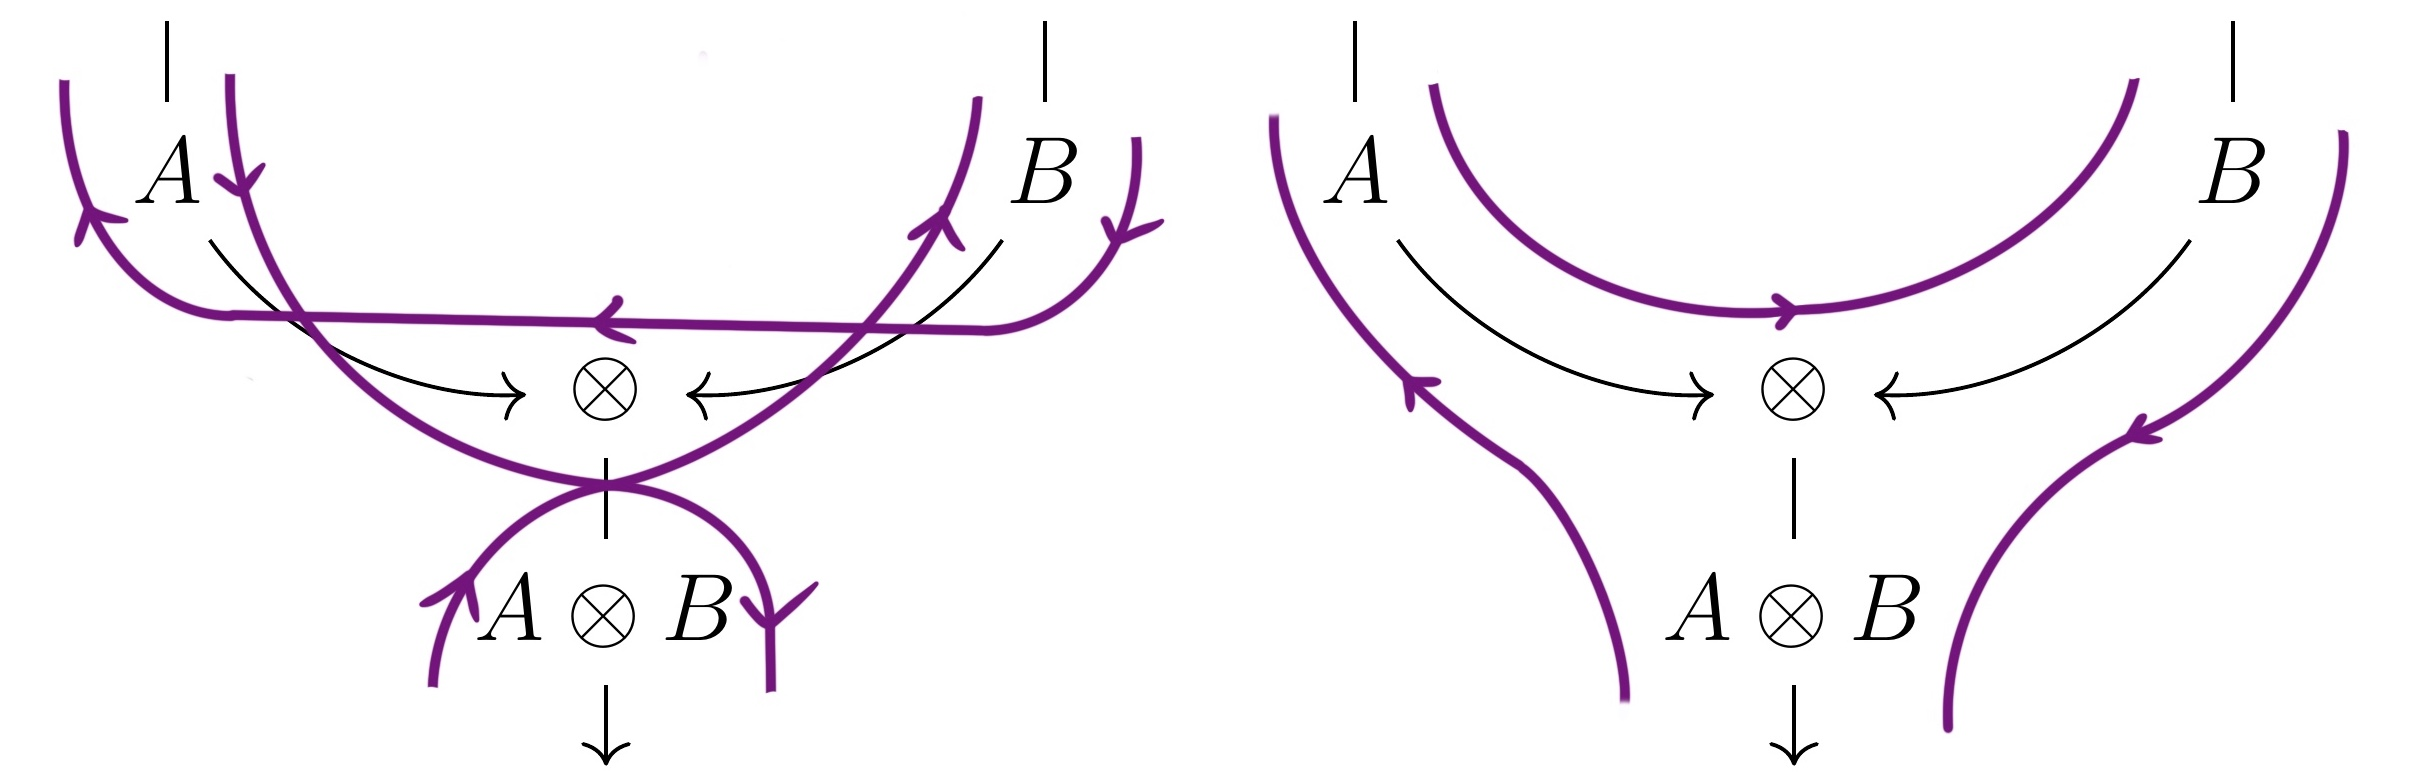
\includegraphics[width = 0.8\textwidth]{TensorSwitch.jpg}
			\caption{Tensor link, $L$ switching, $R$ switching}
			\label{fig:tensorswitching}
		\end{figure}
		\begin{figure}[h]
			\centering
			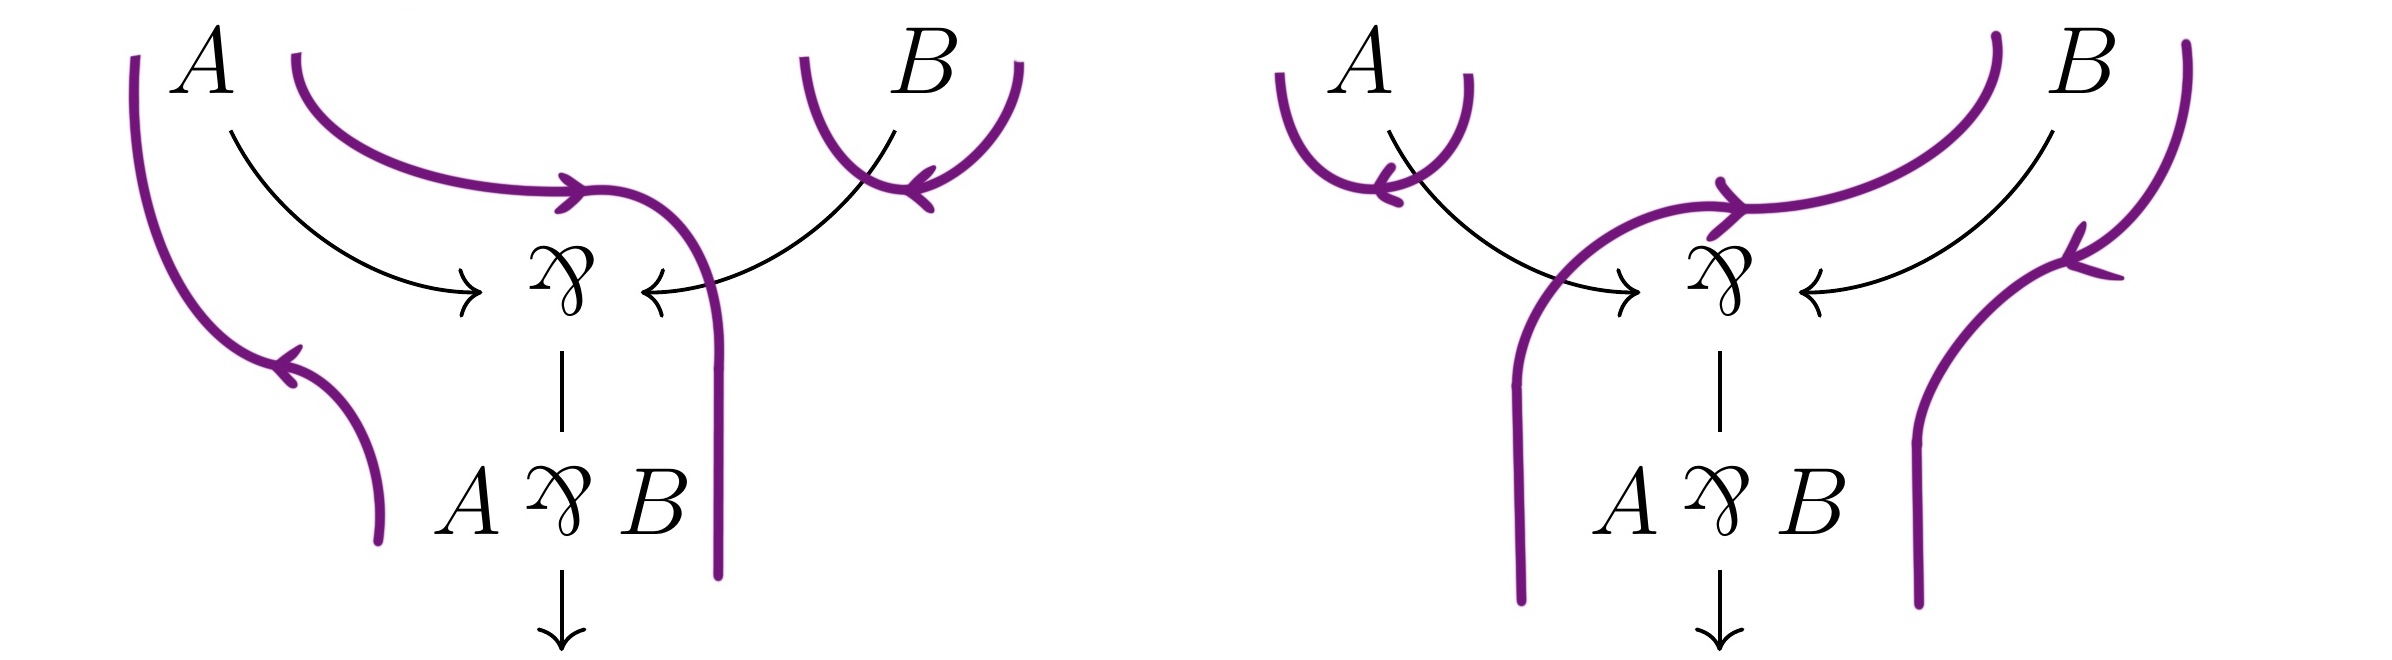
\includegraphics[width = 0.8\textwidth]{ParSwitch.jpg}
			\caption{Par link, $L$ switching, $R$ switching.}
			\label{fig:parrswitching}
		\end{figure}
		\begin{defn}
			Let $\operatorname{Pre}\call{T}(\pi,S)$ denote the set of all pretrips of $\pi$ with respect to $S$. We define an equivalence relation $\sim$ on this set where two pretrips $(x_1,...,x_n)$ and $(y_1,...,y_m)$ are equivalent if $n = m$, and there exists an integer $k$ such that $x_{i + k} = y_i$ (where $i + k$ means $i + k\operatorname{mod} n$) for all $i = 1,...,n$.
			
			A \textbf{trip} of $\pi$ with respect to $S$ is an equivalence class of pretrips. We denote the set of all trips by $\call{T}(\pi,S)$.  If the set $\call{T}(\pi,S)$ admits more than one element, these elements are called \textbf{short trips}, and if it admits only one element, this element is the \textbf{long trip}. We refer to the statement ``for all switchings $S$, the set $\call{T}(\pi,S)$ contains exactly one element" as the \textbf{long trip condition}.
			
			A \textbf{short pretrip} is a choice of representative for a short trip, and a \textbf{long pretrip} is a choice of representatitive of a long trip.
		\end{defn}
		
	\end{defn}
	Given a proof structure $\pi$ satisfying the long trip condition and a tensor link $l$ with premises $A,B$ say, let $S$ be a switching of $\pi$ and $t := (x_1,...,x_n)$ be the long pretrip of $\pi$ satisfying $x_1 =A\downarrow$. Since $\pi$ satisfies the long trip condition, it must be the case that $\uparrow (A \otimes B)$ and $B\downarrow$ occur somewhere in $t$. Can we determine which occurs earlier? Let $m,l > 0$ be such that $x_m = \uparrow (A \otimes B), x_l = B\downarrow$ and assume $l < m$. Say $S(\tau) = L$, then $t$ has the shape
	\begin{equation}\label{eq:sequence_left_switch_tensor}
		(A\downarrow, (A \otimes B)\downarrow, ..., B \downarrow, \uparrow A, ..., \uparrow (A \otimes B), \uparrow B, ..., A\downarrow)
	\end{equation}
	Now consider the switching given by
	\[\hat{S}(\sigma) = \begin{cases}
		S(\sigma),& \sigma \neq \tau\\
		R, & \sigma = \tau
	\end{cases}
	\]
	Then \eqref{eq:sequence_left_switch_tensor} becomes:
	\begin{equation}
		(A\downarrow, \uparrow B, ..., A\downarrow)
	\end{equation}
	which is a short pretrip, contradicting the assumption that $\pi$ satisfies the long trip condition. Thus $m < l$. We have proven (the first half) of the following.
	\begin{lemma}\label{lem:stays_contained_tensor}
		Let $\pi$ be a proof structure satisfying the long trip condition, $l$ be a tensor link with premises $A,B$ say, $S$ be a switching of $\pi$ and $(x_1,...,x_n)$ the long pretrip satisfying $x_1 = A \downarrow$. If $m,l > 0$ are such that $x_m = \uparrow (A \otimes B), x_l = B \downarrow$, then:
		\begin{itemize}
			\item if $S(\tau) = L$ then $m < l$,
			\item if $S(\tau) = R$ then $l < m$.
		\end{itemize}
	\end{lemma}
	The proof of the other half is similar to what has already been written, however since Lemma \ref{lem:stays_contained_tensor} contradicts \cite[Lemma 2.9.1]{linearlogic} we write out the details here:
	\begin{proof}
		Say $m < l$, then $t$ has the shape
		\begin{equation}\label{eq:sequence_right_switch_tensor}
			(A\downarrow, \uparrow B, ..., \uparrow (A \otimes B), \uparrow A, ..., B \downarrow, (A \otimes B)\downarrow, ..., A\downarrow)
		\end{equation}
		Now consider the switching given by
		\[
		S'(\sigma) = 
		\begin{cases}
			S(\sigma),& \sigma \neq \tau\\
			L, & \sigma = \tau
		\end{cases}
		\]
		Then \eqref{eq:sequence_right_switch_tensor} becomes:
		\begin{equation}
			(A\downarrow, (A \otimes B)\downarrow,..., A\downarrow)
		\end{equation}
		which is a short pretrip.
	\end{proof}
	\begin{lemma}\label{lem:stays_contained_par}
		Let $\pi$ be a proof structure satisfying the long trip condition, $l$ be a par link with premises $A,B$ say, $S$ be a switching of $\pi$ and $(x_1,...,x_n)$ be the long pretrip satisfying $x_1 = A\downarrow$. If $m,l > 0$ are such that $x_m = \uparrow (A \parr B), x_l = B\downarrow$, then
		\begin{itemize}
			\item if $S(\tau) = L$ then $m < l$,
			\item if $S(\tau) = R$ then $l < m$
		\end{itemize}
	\end{lemma}
	\begin{remark}
		Lemma \ref{lem:stays_contained_tensor} gives a nice interpretation of Lemma \ref{lem:stays_contained_tensor} that long trips \emph{return to where they left} at each tensor link.
		
		The situation is a bit different for par links; the relevant slogan is long trips \emph{visit the premises before returning to the conclusion}.
	\end{remark}
	Say $\pi$ satisfies the long trip condition and moreover $\pi$ admits a tensor link $l$ (with premises $A,B$ say) such that if $l$ is removed, the resulting proof structure consists of two disjoint proof structures $\pi_1,\pi_2$ each satisfying the long trip condition. It is necessarily the case that any pretrip $\rho$ of $\pi$ starting at $\uparrow A$ visits the entirety of $\call{U}(\pi_1)$ before returning to the tensor link $l$, lest $\pi_1$ admit a short trip. Moreover, it must be the case that $\sigma$ admits no occurrence of formulas in $\pi_2$ lest the result of removing the tensor link $l$ not result in disjoint proof structures. Thus, if such a link $l$ exists, it is \emph{maximal} in the sense that there is no other tensor link $l'$ where a pretrip starting at a premise of $l'$ contains the entirety of any pretrip starting at $A$. Most of the remainder of this Section will amount to proving the converse, that any such maximal tensor link ``splits" $\pi$. This is the \emph{splitting lemma} of \cite{linearlogic}. We then conclude with the Sequentialisation Theorem (Theorem \ref{thm:sequentialisation}).
	\begin{defn}\label{def:pretrip_from_A}
		Let $\pi$ be a proof structure satisfying the long trip condition, $S$ a switching of $\pi$, and $A$ an occurrence of a formula in $\pi$. Consider the long pretrip $(x_1,...,x_n)$ satisfying $x_1 = \uparrow A$. We denote by
		\begin{equation}
			\operatorname{PTrip}(\pi,S,A,\uparrow)
		\end{equation}
		the subsequence $(x_1,...,x_m)$ of $(x_1,...,x_n)$ satisfying $x_m = A\downarrow$. We define
		\begin{equation}
			\operatorname{PTrip}(\pi, S, A, \downarrow)
		\end{equation}
		similarly.
		
		Also, for $a \in \lbrace \uparrow,\downarrow\rbrace $ we define the following set
		\begin{equation}
			\operatorname{Visit}_S(A,a) := \lbrace C \in \call{O}(\pi) \mid \uparrow C, C\downarrow \text{ occur in } \operatorname{PTrip}(\pi,S,A,a)\rbrace
		\end{equation}
		The \textbf{up empire of $A$} is the following set:
		\begin{equation}
			\operatorname{Emp}_{\uparrow}A := \lbrace C \in \call{O}(\pi) \mid \text{For all switchings }S\text{ we have } \uparrow C, C\downarrow \text{ occur in } \operatorname{PTrip}(\pi,S, A,\uparrow)\rbrace
		\end{equation}
		The \textbf{down empire of $A$} is defined symmetrically.
	\end{defn}

One point of difference between the proof presented here and the original proof \cite{linearlogic} is that Girard did \emph{not} consider \emph{down} empires, and instead only considered up empires. At the time of writing, the current author does \emph{not} see how to avoid down empires, and believes the proof in \cite{linearlogic} is too turse to extract a rigorous proof which avoids them.

With the new terminology, we now have some corollaries of Lemmas \ref{lem:stays_contained_tensor} and \ref{lem:stays_contained_par}:
	\begin{cor}\label{cor:pretrip_innards}
		Let $\pi$ be a proof structure satisfying the long trip condition, and let $S$ be a switching of $\pi$, for a formula $A$ and $a \in \lbrace \uparrow, \downarrow\rbrace$, denote $\operatorname{PTrip}(\pi,S, A, a)$ by $\operatorname{PTrip}(A,a)$:
		\begin{enumerate}
			\item if $A$ is part of an axiom link then
			\begin{equation}
				\operatorname{PTrip}(A,\uparrow) = \uparrow A, \operatorname{PTrip}(\neg A, \downarrow), A \downarrow
			\end{equation}
			\item if $l$ is a tensor link with conclusion $A \otimes B$:
			\begin{enumerate}
				\item if $S(l) = L$:
				\begin{equation}
					\operatorname{Ptrip}(A, \downarrow) = A\downarrow, \operatorname{PTrip}(A \otimes B, \downarrow), \operatorname{PTrip}(B, \uparrow), \uparrow A
				\end{equation}
				\begin{equation}
					\operatorname{PTrip}(B, \downarrow) = B\downarrow, \operatorname{PTrip}(A,\uparrow), \operatorname{PTrip}(A \otimes B, \downarrow), \uparrow B
				\end{equation}
				\begin{equation}
					\operatorname{PTrip}(A \otimes B, \uparrow) = \uparrow A \otimes B, \operatorname{PTrip}(B, \uparrow), \operatorname{PTrip}(A,\uparrow), A \otimes B \downarrow
				\end{equation}
				\item if $S(l) = R$:
				\begin{equation}
					\operatorname{PTrip}(A, \downarrow) = A\downarrow, \operatorname{PTrip}(B, \uparrow),\operatorname{PTrip}(A \otimes B, \downarrow), \uparrow A
				\end{equation}
				\begin{equation}
					\operatorname{PTrip}(B, \downarrow) = B\downarrow,  \operatorname{PTrip}(A \otimes B, \downarrow), \operatorname{PTrip}(A,\uparrow),\uparrow B
				\end{equation}
				\begin{equation}
					\operatorname{PTrip}(A \otimes B, \uparrow) = \uparrow A \otimes B,  \operatorname{PTrip}(A,\uparrow), \operatorname{PTrip}(B, \uparrow),A \otimes B \downarrow
				\end{equation}
			\end{enumerate}
			\item if $A$ is a premise of a par link $l$ with conclusion $A \parr B$:
			\begin{enumerate}
				\item if $S(l) = L$:
				\begin{equation}
					\operatorname{PTrip}(A,\downarrow) = A\downarrow, \operatorname{PTrip}(A \parr B, \downarrow), \uparrow A
				\end{equation}
				\begin{equation}
					\operatorname{PTrip}(B, \downarrow) = B\downarrow, \uparrow B
				\end{equation}
				\begin{equation}
					\operatorname{PTrip}(A \parr B, \uparrow) = \uparrow A \parr B, \operatorname{PTrip}(A, \uparrow), A \parr B \downarrow
				\end{equation}
				\item if $S(l) = R$:
				\begin{equation}
					\operatorname{PTrip}(A,\downarrow) = A\downarrow, \uparrow A
				\end{equation}
				\begin{equation}
					\operatorname{PTrip}(B, \downarrow) = B\downarrow, \operatorname{PTrip}(A \parr B, \downarrow), \uparrow B
				\end{equation}
				\begin{equation}
					\operatorname{PTrip}(A \parr B, \uparrow) = \uparrow A \parr B, \operatorname{PTrip}(B, \uparrow), A \parr B \downarrow
				\end{equation}
			\end{enumerate}
		\end{enumerate}
	\end{cor}
	In particular:
	\begin{cor}\label{cor:stays_contained_corollary}
		For any formula $A$ which is a premise to either a tensor or par link, and any $a \in \lbrace \uparrow, \downarrow \rbrace$, we have: $$\uparrow C \text{ occurs in } \operatorname{PTrip}(\pi,S,A,\uparrow)\qquad\text{ if and only if }\qquad C\downarrow \text{ occurs in } \operatorname{PTrip}(\pi,S,A,\downarrow)$$ and similarly for $\operatorname{PTrip}(\pi,S,A,\downarrow)$.
	\end{cor}
	\begin{proof}
		By induction on the length of the sequence $\operatorname{PTrip}(\pi,S,A,a)$ and appealing to Corollary \ref{cor:pretrip_innards}.
	\end{proof}
	\begin{cor}\label{cor:empire_features}
		Let $\pi$ be a proof structure satisfying the long trip condition,
		we have the following.
		\begin{enumerate}
			\item\label{cor:empire_features_up_ax} For any axiom link with conclusions $A, \neg A$:
			\begin{equation}
				\operatorname{Emp}_{\uparrow}A = \operatorname{Emp}_{\downarrow}(\neg A) \cup \lbrace A \rbrace
			\end{equation}
			\item\label{cor:empire_features_down_cut} For any cut link with premises $A, \neg A$:
			\begin{equation}
				\operatorname{Emp}_{\downarrow}A = \operatorname{Emp}_{\uparrow}(\neg A) \cup \lbrace A \rbrace
			\end{equation}
			\item\label{cor:empire_features_empty_int} For any tensor link with premises $A,B$:
			\begin{equation}
				\operatorname{Emp}_{\uparrow}A \cap \operatorname{Emp}_{\uparrow}B = \varnothing
			\end{equation}
			\item\label{cor:empire_features_up_tens_par} For any tensor or par link with premises $A,B$ and conclusion $C$:
			\begin{equation}
				\operatorname{Emp}_{\uparrow}C = \operatorname{Emp}_{\uparrow}A \cup \operatorname{Emp}_{\uparrow}B \cup \lbrace C \rbrace
			\end{equation}
			\item\label{cor:empire_features_down_tens} For any tensor link with premises $A,B$:
			\begin{equation}
				\operatorname{Emp}_{\downarrow}B = \operatorname{Emp}_{\uparrow}A \cup \operatorname{Emp}_{\downarrow}(A \otimes B) \cup \lbrace B \rbrace
			\end{equation}
			and similarly:
			\begin{equation}
				\operatorname{Emp}_{\downarrow}A = \operatorname{Emp}_{\uparrow}B \cup \operatorname{Emp}_{\downarrow}(A \otimes B) \cup \lbrace A\rbrace
			\end{equation}
		\end{enumerate}
	\end{cor}
	\begin{defn}
		Given any link $l$ we write $B \in l$ if $B$ occurs as either a premise or a conclusion of $l$.
		
		Let $\pi$ be a proof structure satisfying the long trip condition, and $a \in \lbrace \uparrow, \downarrow\rbrace$. The set of \textbf{links of $A$ with respect to $S$} is the set
		\begin{equation}
			\operatorname{Link}_aA := \lbrace l \in \operatorname{Link}\pi \mid \forall B \in l, B \in \operatorname{Emp}_aA \rbrace
		\end{equation}
	\end{defn}
	\begin{defn}
		Let $\pi$ be a proof structure satisfying the long trip condition and let $a \in \lbrace \uparrow, \downarrow \rbrace$. Define the set
		\begin{equation}
			\operatorname{Link}^0_{\parr,a}A := \lbrace l \in \operatorname{Link}\pi \mid \text{Exactly one premise of }l\text{ is in }\operatorname{Emp}_{a}A\rbrace
		\end{equation}
	\end{defn}
	\begin{lemma}[Realisation Lemma]\label{lem:realisation_switching}
		Let $\pi$ be a cut-free proof structure satisfying the long trip condition, let $a \in \lbrace \uparrow, \downarrow \rbrace$ and $A$ an occurrence of a formula in $\pi$. Define the following function:
		\begin{align*}
			S: \operatorname{Link}_{\parr,a}^0A &\lto \lbrace L,R\rbrace\\
			l &\longmapsto
			\begin{cases}
				L, & \text{if the right premise of }l\text{ is in }\operatorname{Emp}_{a}A\\
				R, & \text{if the left premise of }l\text{ is in }\operatorname{Emp}_{a}A
			\end{cases}
		\end{align*}
		and extend this to a switching $\hat{S}: \operatorname{Link}\pi \lto \lbrace L,R \rbrace$ arbitrarily. Then
		\begin{equation}
			\operatorname{Emp}_aA = \operatorname{Visit}_{\hat{S}}(A,a)
		\end{equation}
	\end{lemma}
	\begin{proof}
		We proceed by induction on the size $|\operatorname{Link}_a(A)|$ of the set $\operatorname{Link}_a(A)$. For the base case, assume $|\operatorname{Link}_a(A)| = 0$. The formula $A$ is part of an axiom link and so $\operatorname{Emp}_{\uparrow}A = A, \negation A$ and $\operatorname{Emp}_{\downarrow}A = A$, the result follows easily.
		
		Now assume that $|\operatorname{Link}_a A| = n > 0$ and the result holds for any formula $B$ such that $|\operatorname{Link}_aB| < n$. First say $a = \uparrow$, and $A$ is a conclusion of either a tensor or a par link
		% https://q.uiver.app/?q=WzAsNSxbMCwwLCJBXzEiXSxbMiwwLCJBXzIiXSxbMSwxLCJcXGJveHRpbWVzIl0sWzEsMiwiQSJdLFsxLDMsIlxcdmRvdHMiXSxbMyw0XSxbMSwyLCIiLDAseyJjdXJ2ZSI6LTJ9XSxbMCwyLCIiLDIseyJjdXJ2ZSI6Mn1dLFsyLDMsIiIsMCx7InN0eWxlIjp7ImhlYWQiOnsibmFtZSI6Im5vbmUifX19XV0=
		\[\begin{tikzcd}
			{A_1} && {A_2} \\
			& \boxtimes \\
			& A \\
			& \vdots
			\arrow[from=3-2, to=4-2]
			\arrow[curve={height=-12pt}, from=1-3, to=2-2]
			\arrow[curve={height=12pt}, from=1-1, to=2-2]
			\arrow[no head, from=2-2, to=3-2]
		\end{tikzcd}\]
		where $\boxtimes \in \lbrace \otimes, \parr \rbrace$ and $A = A_1 \otimes A_2$ or $A = A_1 \parr A_2$. By \eqref{cor:empire_features_up_tens_par} we have
		\begin{align*}
			\operatorname{Emp}_{\uparrow}A &= \operatorname{Emp}_{\uparrow}A_1 \cup \operatorname{Emp}_{\uparrow}A_2 \cup \lbrace A\rbrace\\
			&= \operatorname{Visit}_{\hat{S}}(A_1,\uparrow) \cup \operatorname{Visit}_S(A_2,\uparrow) \cup \lbrace A \rbrace\\
			&= \operatorname{Visit}_{\hat{S}}(A, \uparrow)
		\end{align*}
		where the second equality follows from the inductive hypothesis.
		
		Assume $A$ is part of an axiom link. By \eqref{cor:empire_features_up_ax}
		\begin{equation}
			\operatorname{Emp}_{\uparrow}A = \operatorname{Emp}_{\downarrow}(\neg A) \cup \lbrace A \rbrace
		\end{equation}
		with
		\begin{equation}
			|\operatorname{Link}_{\uparrow}A| = |\operatorname{Link}_{\downarrow}(\neg A)|
		\end{equation}
		Since $|\operatorname{Link}_{\downarrow}(\negation A)| > 0$ we necessarily have that $\negation A$ is not a conclusion. Thus, since $\pi$ is cut-free, $A$ is connected to an occurrence $\negation A$ which is a premise to either a tensor link or a par link. In the case of the former, we have:
		% https://q.uiver.app/?q=WzAsNSxbMCwwLCJDIl0sWzIsMCwiXFxuZWcgQSJdLFsxLDEsIlxcb3RpbWVzIl0sWzEsMiwiQyBcXG90aW1lcyBcXG5lZyBBIl0sWzEsMywiXFx2ZG90cyJdLFszLDRdLFsxLDIsIiIsMCx7ImN1cnZlIjotMiwic3R5bGUiOnsiaGVhZCI6eyJuYW1lIjoibm9uZSJ9fX1dLFswLDIsIiIsMix7ImN1cnZlIjoyLCJzdHlsZSI6eyJoZWFkIjp7Im5hbWUiOiJub25lIn19fV0sWzIsM11d
		\[\begin{tikzcd}[row sep = small, column sep = small]
			C && {\neg A} \\
			& \otimes \\
			& {C \otimes \neg A} \\
			& \vdots
			\arrow[from=3-2, to=4-2]
			\arrow[curve={height=-12pt}, from=1-3, to=2-2]
			\arrow[curve={height=12pt}, from=1-1, to=2-2]
			\arrow[from=2-2, to=3-2, no head]
		\end{tikzcd}\]
		then by \eqref{cor:empire_features_down_tens}:
		\begin{align*}
			\operatorname{Emp}_{\downarrow}(\neg A) &= \operatorname{Emp}_{\uparrow}C \cup \operatorname{Emp}_{\downarrow}(C \otimes \neg A) \cup \lbrace \neg A\rbrace\\
			&= \operatorname{Visit}_{\hat{S}}(C,\uparrow) \cup \operatorname{Visit}_{\hat{S}}(C \otimes \neg A,\downarrow) \cup \lbrace \neg A\rbrace\\
			&= \operatorname{Visit}_{\hat{S}}(\neg A, \downarrow)
		\end{align*}
		where the second equality follows from the inductive hypothesis.
		
		If $\negation A$ is a premise of a par link
		\[\begin{tikzcd}[column sep = small, row sep = small]
			C && {\neg A} \\
			& \parr \\
			& {C \parr \neg A} \\
			& \vdots
			\arrow[from=3-2, to=4-2]
			\arrow[curve={height=-12pt}, from=1-3, to=2-2]
			\arrow[curve={height=12pt}, from=1-1, to=2-2]
			\arrow[from=2-2, to=3-2, no head]
		\end{tikzcd}\]
		then by construction of $\hat{S}$, where we use the specific definition of $S$ for the first time,
		\begin{align*}
			\operatorname{Emp}_{\downarrow}(\neg A) &= \lbrace \neg A\rbrace\\
			&= \operatorname{Visit}_{\hat{S}}(\neg A,\downarrow)
		\end{align*}
		The case when $a = \downarrow$ is exactly similar and so we omit the proof.
	\end{proof}
	\begin{defn}
		A tensor or par link is \textbf{terminal} if it is a conclusion.
	\end{defn}
	\begin{cor}\label{lem:par_link_existence}
		Let $\pi$ be a cut-free proof structure satisfying the long trip condition. Let
		\[l = \begin{tikzcd}[column sep = small, row sep = small]
			A && {B} \\
			& \otimes \\
			& {A \otimes B} \\
			& \operatorname{c}
			\arrow[from=3-2, to=4-2]
			\arrow[curve={height=-12pt}, from=1-3, to=2-2]
			\arrow[curve={height=12pt}, from=1-1, to=2-2]
			\arrow[from=2-2, to=3-2, no head]
		\end{tikzcd}\]
		be a terminal tensor link of $\pi$. Then $\pi$ admits a par link
		\[l' := \begin{tikzcd}[column sep = small, row sep = small]
			C && {D} \\
			& \otimes \\
			& {C \parr D} \\
			& \vdots
			\arrow[from=3-2, to=4-2]
			\arrow[curve={height=-12pt}, from=1-3, to=2-2]
			\arrow[curve={height=12pt}, from=1-1, to=2-2]
			\arrow[from=2-2, to=3-2, no head]
		\end{tikzcd}\]
		such that either $C \in \operatorname{Emp}_{\uparrow}A$ and $D \in \operatorname{Emp}_{\uparrow}B$ or $C \in \operatorname{Emp}_{\uparrow}B$ and $D \in \operatorname{Emp}_{\uparrow}A$ if and only if for any switching $S$ of $\pi$ we have that either
		\[\operatorname{Emp}_{\uparrow}A \subsetneq \operatorname{Visit}_S(A,\uparrow)\qquad\text{or}\qquad \operatorname{Emp}_{\uparrow}B \subsetneq \operatorname{Visit}_S(B,\uparrow)\]
	\end{cor}
	\begin{proof}
		Say $\pi$ admitted $l'$ and $C \in \operatorname{Emp}_{\uparrow}A$ and $D \in \operatorname{Emp}_{\uparrow}B$. If the switching $S$ is such that $S(l) = L$ then $C \parr D \in \operatorname{Visit}_S(B)\setminus \operatorname{Emp}_{\uparrow}B$ and if $S(\tau) = R$ then $C \parr D \in \operatorname{Visit}_S(A) \setminus \operatorname{Emp}_{\uparrow}A$. The other case is similar.
		
		Conversely, say $\pi$ admits no such par link $l'$, that is, assume
		\begin{equation}
			\operatorname{Link}^0_{\parr,\uparrow}(A) \cap \operatorname{Link}^0_{\parr,\uparrow}(B) = \varnothing
		\end{equation}
		Then there is by Lemma \ref{lem:realisation_switching} a well defined function $$S: \operatorname{Link}_{\parr,\uparrow}^0(A) \cup \operatorname{Link}^0_{\parr,\uparrow}(B) \lto \lbrace L, R \rbrace$$ which extends to a switching $\hat{S}$ such that
		\begin{equation}
			\operatorname{Emp}_{\uparrow}A = \operatorname{Visit}_{\hat{S}}(A,\uparrow)\qquad\text{and}\qquad \operatorname{Emp}_{\uparrow}B = \operatorname{Visit}_{\hat{S}}(B,\uparrow)
		\end{equation}
	\end{proof}
	
	\begin{lemma}[Separation Lemma]
		A cut-free proof structure $\pi$ satisfying the long trip condition, with only tensor links amongst its conclusions admits a tensor link
		\[l := \begin{tikzcd}[column sep = small, row sep = small]
			A && {B} \\
			& \otimes \\
			& {A \otimes B} \\
			& \operatorname{c}
			\arrow[from=3-2, to=4-2]
			\arrow[curve={height=-12pt}, from=1-3, to=2-2]
			\arrow[curve={height=12pt}, from=1-1, to=2-2]
			\arrow[from=2-2, to=3-2, no head]
		\end{tikzcd}\]
		satisfying
		\begin{equation}
			\call{O}(\pi) = \operatorname{Emp}_{\uparrow}A \cup \operatorname{Emp}_{\uparrow}B \cup \lbrace A \otimes B\rbrace
		\end{equation}
		Moreover, removing $A \otimes B$ results in a disconnected graph with each component a proof structure satisfying the long trip condition.
	\end{lemma}
	\begin{proof}
		Consider the set of tensor links $\operatorname{Link}_{\otimes}(\pi)$ of $\pi$. We endow this with the following partial order $\leq$: a pair of links:
		\[
		l' := \begin{tikzcd}[column sep = small, row sep = small]
			A && {B} \\
			& \otimes \\
			& {A \otimes B} \\
			& \vdots
			\arrow[from=3-2, to=4-2]
			\arrow[curve={height=-12pt}, from=1-3, to=2-2]
			\arrow[curve={height=12pt}, from=1-1, to=2-2]
			\arrow[from=2-2, to=3-2, no head]
		\end{tikzcd}
		%
		\qquad
		%
		l'' :=
		\begin{tikzcd}[column sep = small, row sep = small]
			C && {D} \\
			& \otimes \\
			& {C \otimes D} \\
			& \vdots
			\arrow[from=3-2, to=4-2]
			\arrow[curve={height=-12pt}, from=1-3, to=2-2]
			\arrow[curve={height=12pt}, from=1-1, to=2-2]
			\arrow[from=2-2, to=3-2, no head]
		\end{tikzcd}
		\]
		are such that $l' \leq l''$ if $\operatorname{Emp}_{\uparrow}A \cup \operatorname{Emp}_{\uparrow}B \subseteq \operatorname{Emp}_{\uparrow}C \cup \operatorname{Emp}_{\uparrow}D$. Let $l$ (with conclusion $A \otimes B$ say) be a tensor link maximal with respect to $\leq$. We show that $l$ satisfies the required property.
		
		Say $\call{O}(\pi) \neq \operatorname{Emp}_{\uparrow}A \cup \operatorname{Emp}_{\uparrow}B \cup \lbrace A \otimes B\rbrace$. Then by Lemma \ref{lem:par_link_existence} there exists a par link
		\[
		l' = \begin{tikzcd}[column sep = small, row sep = small]
			C && {D} \\
			& \parr \\
			& {C \parr D} \\
			& \vdots
			\arrow[from=3-2, to=4-2]
			\arrow[curve={height=-12pt}, from=1-3, to=2-2]
			\arrow[curve={height=12pt}, from=1-1, to=2-2]
			\arrow[from=2-2, to=3-2, no head]
		\end{tikzcd}
		\]
		such that either $C \in \operatorname{Emp}_{\uparrow}A$ and $D \in \operatorname{Emp}_{\uparrow}B$ or $C \in \operatorname{Emp}_{\uparrow}B$ and $D \in \operatorname{Emp}_{\uparrow}A$. We show the proof in the case of the former. Since $\pi$ admits no terminal par links, the unique maximal length directed path of $\pi$ beginning at the node $\parr$ of $l'$ terminates at an edge labelled $E \otimes F$, for some $E,F$.
		\[l'':= \begin{tikzcd}[column sep = small, row sep = small]
			E && {F} \\
			& \otimes \\
			& {E \otimes F} \\
			& \vdots
			\arrow[from=3-2, to=4-2]
			\arrow[curve={height=-12pt}, from=1-3, to=2-2]
			\arrow[curve={height=12pt}, from=1-1, to=2-2]
			\arrow[from=2-2, to=3-2, no head]
		\end{tikzcd}\]
		Notice that if $l'' = l$, then either $C \parr D \in \operatorname{Emp}_{\uparrow}A$ or $C \parr D \in \operatorname{Emp}_{\uparrow}B$ which in either case implies $\operatorname{Emp}_{\uparrow}A \cap \operatorname{Emp}_{\uparrow}B \neq \varnothing$, contradicting Corollary \ref{cor:empire_features}, \ref{cor:empire_features_empty_int}, and so $l'' \neq l$. Without any loss of generality, assume that $l'$ sits above $F$. The situation looks as follows.
		% https://q.uiver.app/?q=WzAsMjEsWzMsMywiQSBcXG90aW1lcyBCIl0sWzMsNSwiXFxvcGVyYXRvcm5hbWV7Y30iXSxbMiwyLCJBIl0sWzIsMSwiXFx2ZG90cyJdLFsxLDAsIlxcYXgiXSxbMCw1LCJDIl0sWzMsNiwiXFxwYXJyIl0sWzYsNSwiRCJdLFszLDcsIkMgXFxwYXJyIEQiXSxbMCwxLCJcXHZkb3RzIl0sWzQsMiwiQiJdLFs0LDEsIlxcdmRvdHMiXSxbNSwwLCJcXGF4Il0sWzYsMSwiXFx2ZG90cyJdLFszLDgsIlxcdmRvdHMiXSxbMyw5LCJGIl0sWzIsMTAsIlxcb3RpbWVzIl0sWzIsMTIsIlxcb3BlcmF0b3JuYW1le2N9Il0sWzIsMTEsIkUgXFxvdGltZXMgRiJdLFsxLDksIkUiXSxbMSw4LCJcXHZkb3RzIl0sWzAsMV0sWzIsMCwiIiwwLHsiY3VydmUiOjJ9XSxbMywyLCIiLDAseyJzdHlsZSI6eyJoZWFkIjp7Im5hbWUiOiJub25lIn19fV0sWzQsMywiIiwwLHsiY3VydmUiOi0yfV0sWzUsNiwiIiwwLHsiY3VydmUiOjJ9XSxbNyw2LCIiLDIseyJjdXJ2ZSI6LTJ9XSxbNiw4LCIiLDIseyJzdHlsZSI6eyJoZWFkIjp7Im5hbWUiOiJub25lIn19fV0sWzQsOSwiIiwyLHsiY3VydmUiOjJ9XSxbOSw1LCIiLDEseyJzdHlsZSI6eyJoZWFkIjp7Im5hbWUiOiJub25lIn19fV0sWzEyLDExLCIiLDEseyJjdXJ2ZSI6Mn1dLFsxMiwxMywiIiwxLHsiY3VydmUiOi0yfV0sWzEzLDcsIiIsMSx7InN0eWxlIjp7ImhlYWQiOnsibmFtZSI6Im5vbmUifX19XSxbOCwxNF0sWzIwLDE5LCIiLDIseyJzdHlsZSI6eyJoZWFkIjp7Im5hbWUiOiJub25lIn19fV0sWzE5LDE2LCIiLDIseyJjdXJ2ZSI6Mn1dLFsxNSwxNiwiIiwwLHsiY3VydmUiOi0yfV0sWzE2LDE4LCIiLDAseyJzdHlsZSI6eyJoZWFkIjp7Im5hbWUiOiJub25lIn19fV0sWzE4LDE3XSxbMTQsMTUsIiIsMSx7InN0eWxlIjp7ImhlYWQiOnsibmFtZSI6Im5vbmUifX19XSxbMTEsMTAsIiIsMSx7InN0eWxlIjp7ImhlYWQiOnsibmFtZSI6Im5vbmUifX19XSxbMTAsMCwiIiwxLHsiY3VydmUiOi0yfV1d
		\[\begin{tikzcd}[column sep = small, row sep = small]
			& \ax &&&& \ax \\
			\vdots && \vdots && \vdots && \vdots \\
			&& A && B \\
			&&& {A \otimes B} \\
			\\
			C &&& {\operatorname{c}} &&& D \\
			&&& \parr \\
			&&& {C \parr D} \\
			& \vdots && \vdots \\
			& E && F \\
			&& \otimes \\
			&& {E \otimes F} \\
			&& {\operatorname{c}}
			\arrow[from=4-4, to=6-4]
			\arrow[curve={height=12pt}, from=3-3, to=4-4]
			\arrow[no head, from=2-3, to=3-3]
			\arrow[curve={height=-12pt}, from=1-2, to=2-3]
			\arrow[curve={height=12pt}, from=6-1, to=7-4]
			\arrow[curve={height=-12pt}, from=6-7, to=7-4]
			\arrow[no head, from=7-4, to=8-4]
			\arrow[curve={height=12pt}, from=1-2, to=2-1]
			\arrow[no head, from=2-1, to=6-1]
			\arrow[curve={height=12pt}, from=1-6, to=2-5]
			\arrow[curve={height=-12pt}, from=1-6, to=2-7]
			\arrow[no head, from=2-7, to=6-7]
			\arrow[from=8-4, to=9-4]
			\arrow[no head, from=9-2, to=10-2]
			\arrow[curve={height=12pt}, from=10-2, to=11-3]
			\arrow[curve={height=-12pt}, from=10-4, to=11-3]
			\arrow[no head, from=11-3, to=12-3]
			\arrow[from=12-3, to=13-3]
			\arrow[no head, from=9-4, to=10-4]
			\arrow[no head, from=2-5, to=3-5]
			\arrow[curve={height=-12pt}, from=3-5, to=4-4]
		\end{tikzcd}\]
		
		
		
		Let $S$ be a switching of $\pi$ so that $\operatorname{Emp}_{\uparrow}F = \operatorname{Visit}_S(F,\uparrow)$ and so that $S(l') = L$, which exists by Lemma \ref{lem:par_link_existence}. Let $t = (x_1,...,x_n)$ be the long pretrip of $\pi$ with respect to $S$ satisfying $x_1 = F\uparrow$. We have by Lemma \ref{lem:stays_contained_par} that $t$ takes the following shape:
		\begin{equation}\label{eq:condemning_shape}
			\uparrow F, ..., \uparrow(C \parr D), \uparrow C, ..., D\downarrow, \uparrow D, ..., C\downarrow, (C \parr D)\downarrow, ..., F\downarrow,...
		\end{equation}
		We have that $D \in \operatorname{Emp}_{\uparrow}B$ so for simplicity, rewrite \eqref{eq:condemning_shape} as $t' = (x_{1 + k},...,x_{n+k})$ for some $k > 0$ (where $i + k$ means $i + k\operatorname{mod} n$) so that $\uparrow B$ occurs to the left of $D \downarrow$ and $B \downarrow$ occurring to the right of $\uparrow D$.
		We have that $C \not\in \operatorname{Emp}_{\uparrow}B$ and so by Corollary \ref{cor:stays_contained_corollary}:
		\begin{equation}
			\uparrow B \text{ occurrs in }\uparrow C,..., D\downarrow\text{ and } B\downarrow\text{ occurrs in }\uparrow D, ..., C\downarrow
		\end{equation}
		However, this implies that $B \in \operatorname{Visit}_S(F,\uparrow)$ which by Lemma \ref{lem:realisation_switching} implies $B \in \operatorname{Emp}_{\uparrow}F$.
		
		By reversing the switching of $l'$ we can similarly show that $A \in \operatorname{Emp}_{\uparrow}F$, contradicting the maximality of $l$. This proves the first claim.
		
		For the second claim, since $\call{O}(\pi) = \operatorname{Emp}_{\uparrow}A \cup \operatorname{Emp}_{\uparrow}B \cup \lbrace A \otimes B\rbrace$ we have by Lemma \ref{lem:par_link_existence} that
		\begin{equation}
			\operatorname{Link}_{\parr,\uparrow}^0(A\otimes B) = \varnothing
		\end{equation}
		and we saw in the proof of Lemma \ref{lem:realisation_switching} that a switching $S$ which realises $\operatorname{Emp}_{\uparrow}A$ is given by setting all switchings arbitrarily except for those in $\operatorname{Link}_{\parr,\uparrow}^0(A\otimes B)$. This means that for any switching $S$ of $\pi$:
		\begin{equation}
			\operatorname{Visit}_{S}(A,\uparrow) = \operatorname{Emp}_{\uparrow}A \qquad\text{and}\qquad \operatorname{Visit}_{S}(B,\uparrow) = \operatorname{Emp}_{\uparrow}B
		\end{equation}
		which is to say the two subproof structures given by removing $A \otimes B$ never admit a short trip, that is, they each satisfy the long trip condition.
	\end{proof}
	\begin{thm}[The Sequentialisation Theorem]\label{thm:sequentialisation}
		A proof structure $\pi$ (possibly with cuts) satisfies the long trip condition if and only $\pi$ is a proof net.
	\end{thm}
	\begin{proof}
		First assume that $\pi$ is cut-free.
		
		We proceed by induction on the size $|\operatorname{Link}\pi|$ of the set $\operatorname{Link}\pi$. If there this is zero then $\pi$ consists of a single axiom link and so the result is clear.
		
		For the inductive step, we consider two cases, first say $\pi$ admits a par link for a conclusion. Then removing this par link clearly results in two cut-free subproof structures satsifying the long trip condition and so the result follows from the inductive hypothesis. If no such terminal par link exists, then by the Separation Lemma there exists some tensor link in the conclusion for which we can remove and apply the inductive hypothesis.
		
		Now say that $\pi$ contained cuts. We replace each cut with a tensor link to create a new proof $\zeta$. That there exists a proof $\Xi$ which maps to $\zeta$ follows from the part of the result proved already as $\zeta$ is cut-free. We adapt $\Xi$ appropriately by replacing $\otimes$-rules by $\operatorname{cut}$-rules and we are done.
	\end{proof}
	
	\subsection{Modelling the dynamics of MLL}
	The distinction between \emph{sense} and \emph{reference}, due to Frege \cite{Frege}, can crudely be explained as the \emph{means of description} of an object vs the object itself. From this angle, it makes sense to ignore the distinction between two proofs which differ only by a series of cut-reduction steps (either forwards or backwards ones), as surely these two proofs do not differ in their reference. This is the \emph{denotational semantics} program, in which two proofs $\pi, \pi'$ which are cut-equivalent to each other are given the same interpretation $\llbracket \pi \rrbracket = \llbracket \pi' \rrbracket$.
	
	On the other hand, the Curry-Howard correspondence \cite{Sorensen} and the Gentzen-Mints-Zucker Duality \cite{GMZ} relate the cut-elimination process to the dynamics of a system of computation ($\beta$-reduction in the simply typed $\lambda$-calculus, in both cases). Thus, it makes sense also to look for models of logical systems where two cut equivalent proofs $\pi, \pi'$ are \emph{not} given the same interpretation, but instead there exists some relationship between the two $\llbracket \pi \rrbracket \lto \llbracket \pi' \rrbracket$. This is the \emph{geometry of interaction} \cite{multiplicatives}, \cite{girard}, \cite{GoI2}, \cite{GoI3}, \cite{GoI4}, \cite{GoI5}, due to Girard. In this section, we introduce the first two of these models which he created. The reference for Geometry of Interaction Zero is \cite{multiplicatives} and the reference for Geometry of Interaction One is \cite{girard}.
	
	See the Introduction of \cite{Seiller4} for more on the distinction between denotation semantics and Geometry of Interaction.
	
	\begin{defn}\label{def:r}
		Let $\call{F}$ denote the set of formulas (Definition \ref{def:formulas}), $\call{A}$ the set of oriented atoms, and $\call{A}^\ast = \bigcup_{n \geq 0}\call{A}^n$ the set of sequences of oriented atoms of length $\geq 0$. We define an involution $r$ on $\call{A}^\ast$ as follows:
		\begin{align}
			r: \call{A}^\ast &\lto \call{A}^\ast\\
			\big((X_1,x_1),...,(X_n,x_n)\big) &\longmapsto \big((X_n,\bar{x}_n),...,(X_1,\bar{x}_1)\big)
		\end{align}
	where $\overline{+} = -$ and $\overline{-} = +$.
	
		For the empty string $\emptyset \in \call{A}^\ast$ we define $r(\emptyset) = \emptyset$.
		% Given two sequences $(\underline{a_1},...,\underline{a_n}),(\underline{b_1},...,\underline{b_m})$ both in $\call{A}^\ast$ we denote by $(\underline{a_1},...,\underline{a_n})\cdot(\underline{b_1},...,\underline{b_m})$ the concatenation $(\underline{a_1},...,\underline{a_n},\underline{b_1},...,\underline{b_m})$.
	\end{defn}	
	
	The set $\call{A}^\ast$ is a monoid under concatenation $c: \call{A}^\ast \times \call{A}^\ast \lto \call{A}^\ast$ with identity $\emptyset$.
	
	\begin{defn}\label{def:tensor}
		We denote by $\otimes: \call{F} \times \call{F} \lto \call{F}$ the function which maps a pair of formulas $(A,B)$ to the formula $A \otimes B$. Similarly, $\parr: \call{F} \times \call{F} \lto \call{F}$ denotes the function such that $\parr(A,B) = A \parr B$ and $\neg : \call{F} \lto \call{F}$ denotes the function such that $\neg(A) = \neg A$. We denote by $\operatorname{inc}: \call{A} \lto \call{F}$ the map which sends an oriented atom $(X,x)$ to itself $(X,x)$, and lastly we denote by $\operatorname{\iota}: \call{A} \lto \call{A}^\ast$ the function which maps an oriented atom $(X,x)$ to the sequence consisting only of $(X,x)$.
	\end{defn}
	
	\begin{lemma}\label{lem:negation_map}
		There is a unique map $a: \call{F} \lto \call{A}^\ast$ making the following diagrams commute
		\begin{equation}
			\begin{tikzcd}
				\call{F} \times \call{F}\arrow[r,"{a \times a}"] \arrow[d,swap,"{\otimes}"]& \call{A}^\ast \times \call{A}^\ast\arrow[d,"{c}"]\\
				\call{F}\arrow[r,"{a}"] & \call{A}^\ast
			\end{tikzcd}
			%
			\qquad
			%
			\begin{tikzcd}
				\call{F} \times \call{F}\arrow[r,"{a \times a}"]\arrow[d,swap,"{\parr}"] & \call{A}^\ast \times \call{A}^\ast\arrow[d,"{c}"]\\
				\call{F}\arrow[r,"{a}"] & \call{A}^\ast
			\end{tikzcd}
		\end{equation}
		\begin{equation}
			\begin{tikzcd}
				\call{F}\arrow[r,"{a}"]\arrow[d,swap,"{\sim}"] & \call{A}^\ast\arrow[d,swap,"{r}"]\\
				\call{F}\arrow[r,"{a}"] & \call{A}^\ast
			\end{tikzcd}
			%
			\qquad
			%
			\begin{tikzcd}
				\call{A}\arrow[r,"{\operatorname{inc}}"]\arrow[dr,swap,"{\iota}"] & \call{F}\arrow[d,"{a}"]\\
				& \call{A}^\ast
			\end{tikzcd}
		\end{equation}
	\end{lemma}
	\begin{proof}
		Left to the reader.
	\end{proof}
	
	\begin{defn}\label{def:seq_set_two}
		Let $A$ be a formula. The \textbf{sequence of oriented atoms} of $A$ is $a(A) = (X_1,x_1),\ldots,(X_n,x_n)$ as defined by the previous lemma. The \textbf{sequence of unoriented atoms} of $A$ is $X_1,...,X_n$ and the \textbf{set of unoriented atoms} of $A$ is the disjoint union $U_A = \lbrace X_1 \rbrace \coprod \ldots \coprod \lbrace X_n \rbrace$. The \textbf{set of unoriented atoms} of a proof structure $\pi$ is the disjoint union $U_\pi = \coprod_{e \in E}U_{A_e}$ where $E$ is the set of edges of $\pi$, and $A_e$ is the formula labelling $e$.
	\end{defn}
	
	\subsection{Proofs as permutations (Geometry of Interaction Zero)}
A proof $\pi$ in MLL with a single conclusion $A$ is determined by $A$ up to the axiom links of $\pi$. For instance, when the following proof net is read with dashed Axiom links ignored, we obtain a proof net $\pi$, and similarly if we read the dashed Axiom links and with the solid arrow Axiom links ignored.
\begin{example}
		% https://q.uiver.app/?q=WzAsMTUsWzMsNiwiXFxwYXJyIl0sWzEsNSwiQSBcXG90aW1lcyBBIl0sWzUsNSwiXFxuZWcgQSBcXHBhcnIgXFxuZWcgQSJdLFs0LDMsIlxcbmVnIEEiXSxbNiwzLCJcXG5lZyBBIl0sWzIsMywiQSJdLFswLDMsIkEiXSxbNSw0LCJcXHBhcnIiXSxbMSw0LCJcXG90aW1lcyJdLFszLDEsIlxcYXgiXSxbMywwLCJcXGF4Il0sWzQsMiwiXFxheCJdLFsyLDIsIlxcYXgiXSxbMyw3LCIoQSBcXG90aW1lcyBBKSBcXHBhcnIgKFxcbmVnIEEgXFxwYXJyIFxcbmVnIEEpIl0sWzMsOCwiXFxvcGVyYXRvcm5hbWV7Y30iXSxbMSwwLCIiLDAseyJjdXJ2ZSI6Mn1dLFsyLDAsIiIsMix7ImN1cnZlIjotMn1dLFs0LDddLFszLDddLFs3LDIsIiIsMCx7InN0eWxlIjp7ImhlYWQiOnsibmFtZSI6Im5vbmUifX19XSxbNSw4XSxbNiw4XSxbOCwxLCIiLDIseyJzdHlsZSI6eyJoZWFkIjp7Im5hbWUiOiJub25lIn19fV0sWzksMywiIiwwLHsiY3VydmUiOi0xLCJzdHlsZSI6eyJib2R5Ijp7Im5hbWUiOiJkYXNoZWQifSwiaGVhZCI6eyJuYW1lIjoibm9uZSJ9fX1dLFs5LDUsIiIsMSx7ImN1cnZlIjoxLCJzdHlsZSI6eyJib2R5Ijp7Im5hbWUiOiJkYXNoZWQifSwiaGVhZCI6eyJuYW1lIjoibm9uZSJ9fX1dLFsxMCw0LCIiLDIseyJjdXJ2ZSI6LTMsInN0eWxlIjp7ImJvZHkiOnsibmFtZSI6ImRhc2hlZCJ9LCJoZWFkIjp7Im5hbWUiOiJub25lIn19fV0sWzEwLDYsIiIsMSx7ImN1cnZlIjozLCJzdHlsZSI6eyJib2R5Ijp7Im5hbWUiOiJkYXNoZWQifSwiaGVhZCI6eyJuYW1lIjoibm9uZSJ9fX1dLFsxMSw0LCIiLDEseyJjdXJ2ZSI6LTEsInN0eWxlIjp7ImhlYWQiOnsibmFtZSI6Im5vbmUifX19XSxbMTEsNSwiIiwxLHsiY3VydmUiOjMsInN0eWxlIjp7ImhlYWQiOnsibmFtZSI6Im5vbmUifX19XSxbMTIsNiwiIiwxLHsiY3VydmUiOjEsInN0eWxlIjp7ImhlYWQiOnsibmFtZSI6Im5vbmUifX19XSxbMTIsMywiIiwxLHsiY3VydmUiOi0zLCJzdHlsZSI6eyJoZWFkIjp7Im5hbWUiOiJub25lIn19fV0sWzAsMTMsIiIsMCx7InN0eWxlIjp7ImhlYWQiOnsibmFtZSI6Im5vbmUifX19XSxbMTMsMTRdXQ==
		\begin{equation}\label{eq:counter_one}
			\begin{tikzcd}[column sep = tiny, row sep = small]
				&&& \ax \\
				&&& \ax \\
				&& \ax && \ax \\
				X_1 && X_2 && {\neg X_3} && {\neg X_4} \\
				& \otimes &&&& \parr \\
				& {X \otimes X} &&&& {\neg X\parr \neg X} \\
				&&& \parr \\
				&&& {(X\otimes X) \parr (\neg X \parr \neg X)} \\
				&&& {\operatorname{c}}
				\arrow[curve={height=12pt}, from=6-2, to=7-4]
				\arrow[curve={height=-12pt}, from=6-6, to=7-4]
				\arrow[from=4-7, to=5-6]
				\arrow[from=4-5, to=5-6]
				\arrow[no head, from=5-6, to=6-6]
				\arrow[from=4-3, to=5-2]
				\arrow[from=4-1, to=5-2]
				\arrow[no head, from=5-2, to=6-2]
				\arrow[curve={height=-6pt}, dashed, no head, from=2-4, to=4-5]
				\arrow[curve={height=6pt}, dashed, no head, from=2-4, to=4-3]
				\arrow[curve={height=-18pt}, dashed, no head, from=1-4, to=4-7]
				\arrow[curve={height=18pt}, dashed, no head, from=1-4, to=4-1]
				\arrow[curve={height=-6pt}, no head, from=3-5, to=4-7]
				\arrow[curve={height=18pt}, no head, from=3-5, to=4-3]
				\arrow[curve={height=6pt}, no head, from=3-3, to=4-1]
				\arrow[curve={height=-18pt}, no head, from=3-3, to=4-5]
				\arrow[no head, from=7-4, to=8-4]
				\arrow[from=8-4, to=9-4]
			\end{tikzcd}
		\end{equation}
Assuming that $\pi$ satisfies the property that all the conclusions of its axiom links are atomic, then in fact these two possibilities completely exhaust the proof nets with conclusion $(X\otimes X) \parr (\neg X \parr \neg X)$. This example is generic, in the sense that the ``trunk'' of any proof net is completely determined by its conclusion.

A compact way of describing the axiom links of a proof in MLL is to read each axiom link as a transposition, and to give the product of these as a permutation. This translation of proofs into permutations was first given in \cite{multiplicatives} and was expounded upon in \cite{girard}. Due to the popularity of the latter paper, the former is often overlooked.

In \cite{multiplicatives}, it is also shown how to relate the permutations of a proof with cuts to the permutations of the associated normal form. The most important difference between the current presentation and that of \cite{multiplicatives} is that we use \emph{unoriented atoms} (Definition \ref{def:seq_set_two}).
	
	\begin{defn}\label{def:atomic_atoms_ax_concs}
		Let $\pi$ be a proof net. Let $\call{P}(\pi)$ denote the disjoint union of all the unoriented axioms of all formulas which are conclusions to axiom links in $\pi$.
	\end{defn}
		
	\begin{defn}\label{def:permutations}
		Let $\pi$ be a proof net with axiom links $l_1,...,l_n$ say. For each $i = 1,...,n$ the link $l_i$ defines a permutation $\tau_{l_i}$ on the set $\call{P}(\pi)$ in the following way: if $l_i$ has conclusions $\neg A, A$ then the $j^\text{th}$ element of the sequence of unoriented atoms of $A$ is mapped via $\tau_{l_i}$ to the $j^\text{th}$ element of the sequence of unoriented atoms of $\neg A$. We define $\alpha_\pi$ to be the product of all these permutations.
		\begin{equation}
			\alpha_\pi := \tau_{l_1}\hdots \tau_{l_n}
		\end{equation}
		We call this permutation the \textbf{axiom link permutation associated to $\pi$}.
		
		We define more permutations on $\call{P}(\pi)$. Recall the definitions of pretrips (Definition \ref{def:pretrip_from_A}) and switchings (Definition \ref{def:switching}). Let $S$ be a switching of $\pi$. For each unoriented axiom $X \in \call{P}(\pi)$, corresponding to a formula $A$ say, let $\beta_{\pi}^S(X)$ denote the unoriented axiom corresponding to the first occurrence in $\operatorname{PTrip}(\pi,S,A,\downarrow)$ of the form $\uparrow B$ where $B$ is a formula labelling a conclusion of an axiom link in $\pi$.
		
		The set of all permutations of the second form is denoted:
		\begin{equation}
			\Sigma(\pi) := \lbrace \beta_{\pi}^S \mid S\text{ is a switching of }\pi\rbrace
		\end{equation}
		We will often denote elements of $\beta_{\pi}^S \in \Sigma(\pi)$ simply by $\beta$.
	\end{defn}
	\begin{example}\label{ex:counter}
		\begin{figure}[h]
			\centering
			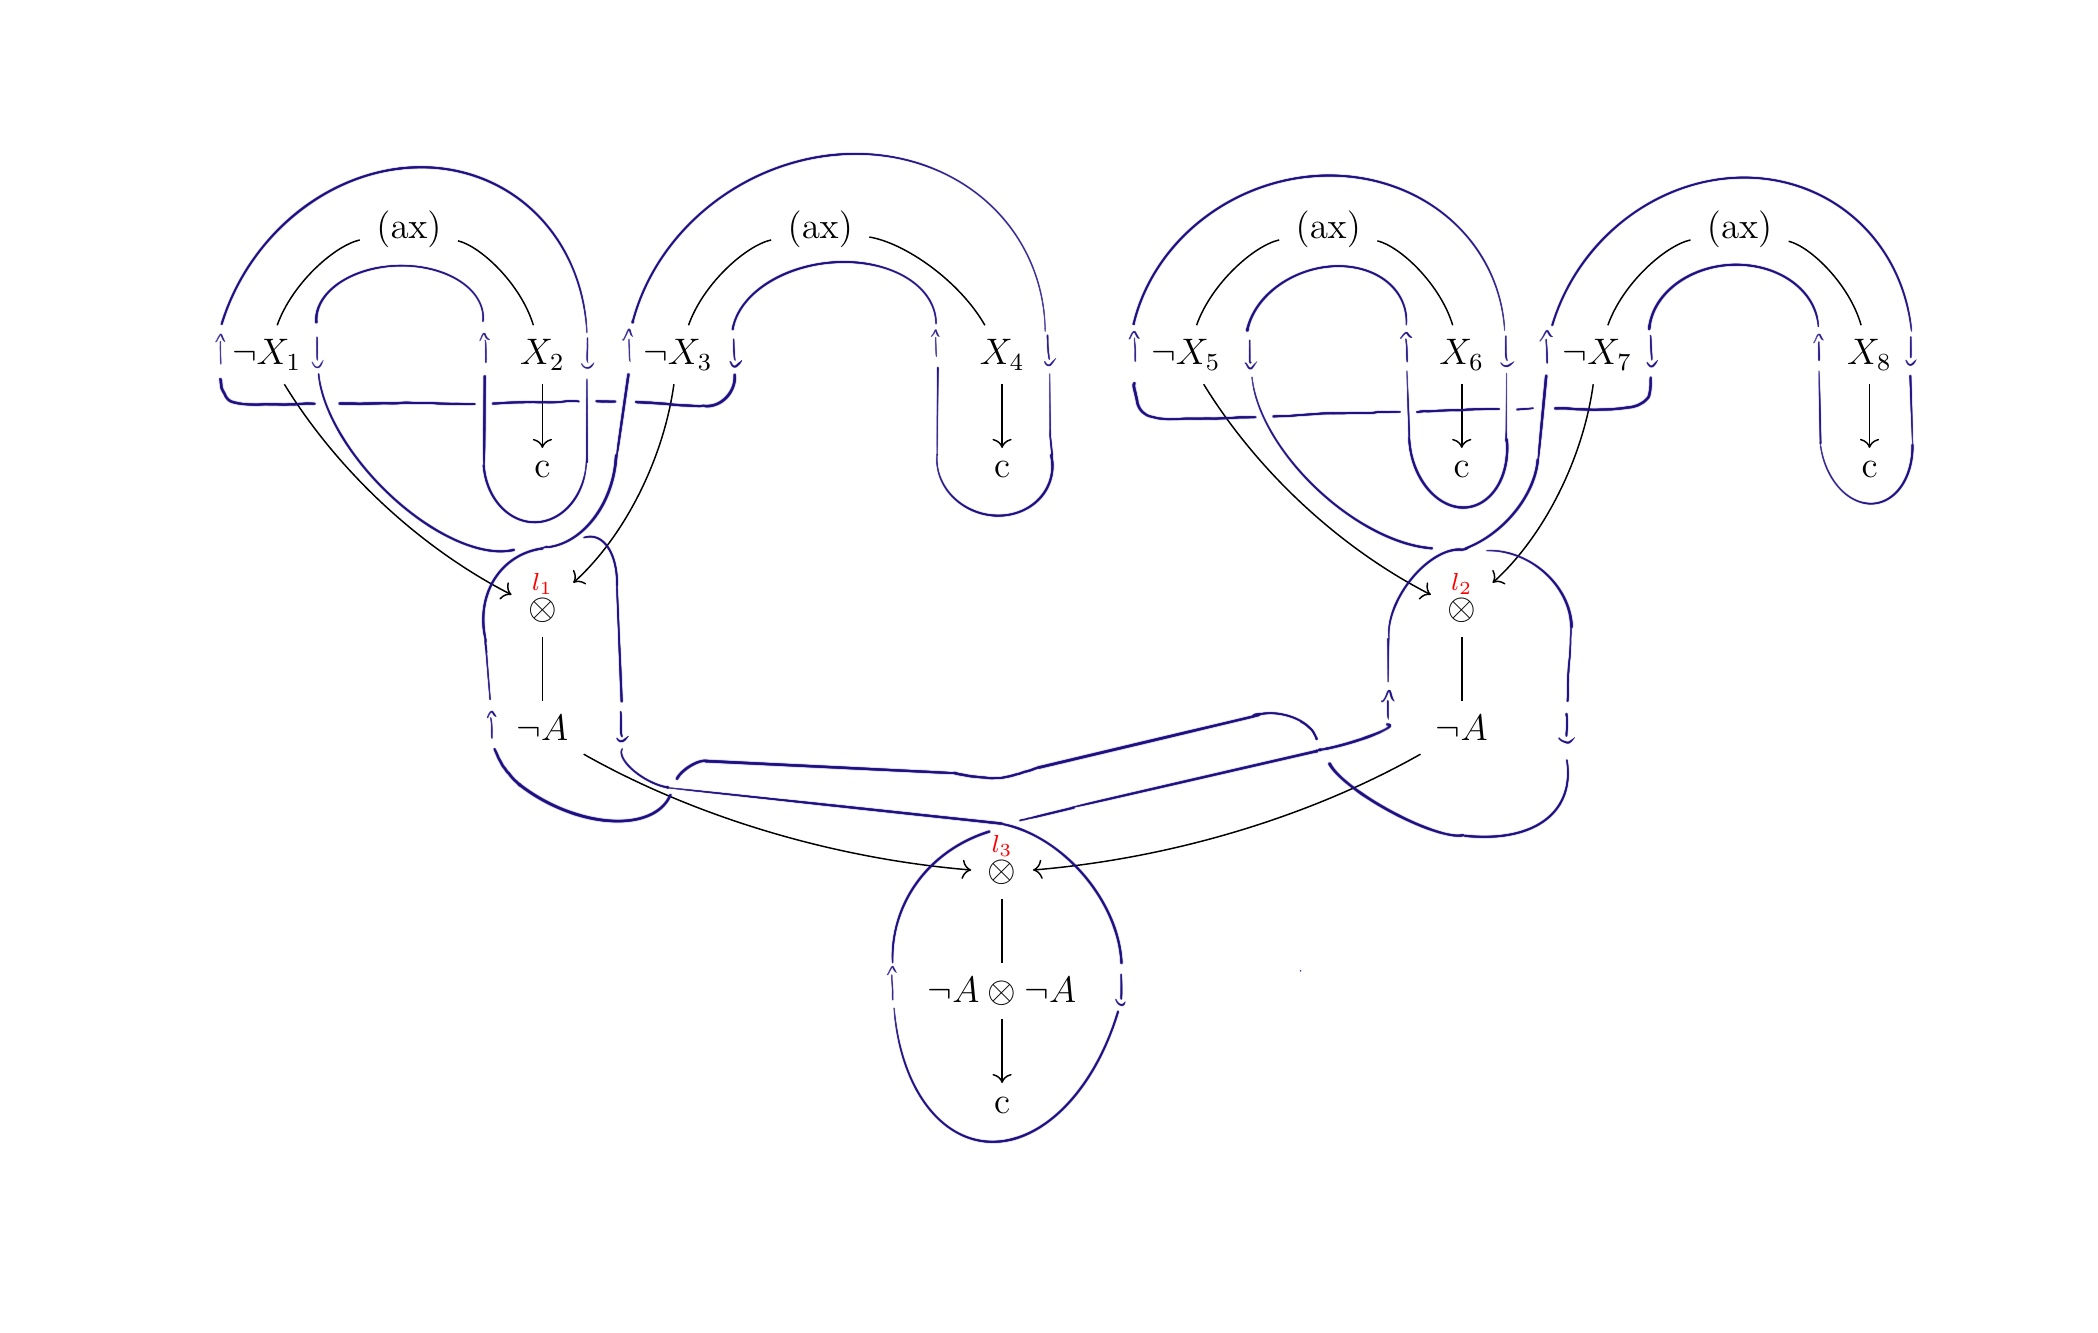
\includegraphics[width = 20cm]{Switching.jpg}
			\caption{The switching $S$ of Example \ref{ex:counter}}
			\label{fig:counter_one}
		\end{figure}
		Let $\pi$ denote the following proof structure with tensor links labelled $l_1, l_2, l_3$ as displayed. The formula $A$ denotes $\neg X \otimes \neg X$.
		% https://q.uiver.app/?q=WzAsMjMsWzAsMSwiXFxuZWcgWF8xIl0sWzIsMSwiWF8yIl0sWzMsMSwiXFxuZWcgWF8zIl0sWzUsMSwiWF80Il0sWzIsMywiXFxvdGltZXMiXSxbMiw0LCJcXG5lZyBBIl0sWzEsMCwiXFxheCJdLFs0LDAsIlxcYXgiXSxbNiwxLCJcXG5lZyBYXzUiXSxbOCwxLCJYXzYiXSxbOSwxLCJcXG5lZyBYXzciXSxbMTEsMSwiWF84Il0sWzEwLDAsIlxcYXgiXSxbNywwLCJcXGF4Il0sWzgsMywiXFxvdGltZXMiXSxbOCw0LCJcXG5lZyBBIl0sWzUsNSwiXFxvdGltZXMiXSxbNSw2LCJcXG5lZyBBIFxcb3RpbWVzIFxcbmVnIEEiXSxbNSw3LCJcXG9wZXJhdG9ybmFtZXtjfSJdLFsyLDIsIlxcb3BlcmF0b3JuYW1le2N9Il0sWzUsMiwiXFxvcGVyYXRvcm5hbWV7Y30iXSxbOCwyLCJcXG9wZXJhdG9ybmFtZXtjfSJdLFsxMSwyLCJcXG9wZXJhdG9ybmFtZXtjfSJdLFswLDQsIiIsMCx7ImN1cnZlIjoyfV0sWzIsNCwiIiwyLHsiY3VydmUiOi0yfV0sWzQsNSwiIiwwLHsic3R5bGUiOnsiaGVhZCI6eyJuYW1lIjoibm9uZSJ9fX1dLFs2LDAsIiIsMCx7ImN1cnZlIjoyLCJzdHlsZSI6eyJoZWFkIjp7Im5hbWUiOiJub25lIn19fV0sWzYsMSwiIiwyLHsiY3VydmUiOi0yLCJzdHlsZSI6eyJoZWFkIjp7Im5hbWUiOiJub25lIn19fV0sWzcsMiwiIiwyLHsiY3VydmUiOjIsInN0eWxlIjp7ImhlYWQiOnsibmFtZSI6Im5vbmUifX19XSxbNywzLCIiLDAseyJjdXJ2ZSI6LTIsInN0eWxlIjp7ImhlYWQiOnsibmFtZSI6Im5vbmUifX19XSxbMTMsOCwiIiwwLHsiY3VydmUiOjIsInN0eWxlIjp7ImhlYWQiOnsibmFtZSI6Im5vbmUifX19XSxbMTMsOSwiIiwyLHsiY3VydmUiOi0yLCJzdHlsZSI6eyJoZWFkIjp7Im5hbWUiOiJub25lIn19fV0sWzEyLDEwLCIiLDIseyJjdXJ2ZSI6Miwic3R5bGUiOnsiaGVhZCI6eyJuYW1lIjoibm9uZSJ9fX1dLFsxMiwxMSwiIiwwLHsiY3VydmUiOi0yLCJzdHlsZSI6eyJoZWFkIjp7Im5hbWUiOiJub25lIn19fV0sWzgsMTQsIiIsMCx7ImN1cnZlIjoyfV0sWzEwLDE0LCIiLDIseyJjdXJ2ZSI6LTJ9XSxbMTQsMTUsIiIsMix7InN0eWxlIjp7ImhlYWQiOnsibmFtZSI6Im5vbmUifX19XSxbNSwxNiwiIiwwLHsiY3VydmUiOjJ9XSxbMTUsMTYsIiIsMix7ImN1cnZlIjotMn1dLFsxNiwxNywiIiwyLHsic3R5bGUiOnsiaGVhZCI6eyJuYW1lIjoibm9uZSJ9fX1dLFsxNywxOF0sWzEsMTldLFszLDIwXSxbOSwyMV0sWzExLDIyXV0=
		\begin{equation}\begin{tikzcd}[column sep = tiny, row sep = small]
			& \ax &&& \ax &&& \ax &&& \ax \\
			{\neg X_1} && {X_2} & {\neg X_3} && {X_4} & {\neg X_5} && {X_6} & {\neg X_7} && {X_8} \\
			&& {\operatorname{c}} &&& {\operatorname{c}} &&& {\operatorname{c}} &&& {\operatorname{c}} \\
			&& \stackrel{\textcolor{red}{l_1}}{\otimes} &&&&&& \stackrel{\textcolor{red}{l_2}}{\otimes} \\
			&& {\neg A} &&&&&& {\neg A} \\
			&&&&& \stackrel{\textcolor{red}{l_3}}{\otimes} \\
			&&&&& {\neg A \otimes \neg A} \\
			&&&&& {\operatorname{c}}
			\arrow[curve={height=12pt}, from=2-1, to=4-3]
			\arrow[curve={height=-12pt}, from=2-4, to=4-3]
			\arrow[no head, from=4-3, to=5-3]
			\arrow[curve={height=12pt}, no head, from=1-2, to=2-1]
			\arrow[curve={height=-12pt}, no head, from=1-2, to=2-3]
			\arrow[curve={height=12pt}, no head, from=1-5, to=2-4]
			\arrow[curve={height=-12pt}, no head, from=1-5, to=2-6]
			\arrow[curve={height=12pt}, no head, from=1-8, to=2-7]
			\arrow[curve={height=-12pt}, no head, from=1-8, to=2-9]
			\arrow[curve={height=12pt}, no head, from=1-11, to=2-10]
			\arrow[curve={height=-12pt}, no head, from=1-11, to=2-12]
			\arrow[curve={height=12pt}, from=2-7, to=4-9]
			\arrow[curve={height=-12pt}, from=2-10, to=4-9]
			\arrow[no head, from=4-9, to=5-9]
			\arrow[curve={height=12pt}, from=5-3, to=6-6]
			\arrow[curve={height=-12pt}, from=5-9, to=6-6]
			\arrow[no head, from=6-6, to=7-6]
			\arrow[from=7-6, to=8-6]
			\arrow[from=2-3, to=3-3]
			\arrow[from=2-6, to=3-6]
			\arrow[from=2-9, to=3-9]
			\arrow[from=2-12, to=3-12]
		\end{tikzcd}
		\end{equation}
	Consider first the switching $S(l_1) = S(l_2) = S(l_3) = L$. Then we have
	\begin{equation}
		\beta_\pi^S: X_1 \mapsto X_7 \mapsto X_5 \mapsto X_3 \mapsto X_1, \quad X_i \mapsto X_i, i = 2,4,6,8
		\end{equation}
	The other permutations are as follows.
	\begin{align*}
		&X_1 \mapsto X_3 \mapsto X_7 \mapsto X_5 \mapsto X_1, \quad X_i \mapsto X_i, i = 2,4,6,8\\
		&X_1 \mapsto X_3 \mapsto X_5 \mapsto X_7 \mapsto X_1, \quad X_i \mapsto X_i, i = 2,4,6,8\\
		&X_1 \mapsto X_5 \mapsto X_7 \mapsto X_3 \mapsto X_1, \quad X_i \mapsto X_i, i = 2,4,6,8
		\end{align*}
	\end{example}
	We can now rephrase the longtrip condition of Section \ref{sec:sequentialisation} in terms of permutations.
	\begin{proposition}
		Let $\pi$ be a proof structure, then $\pi$ is a proof net if and only if for all $\beta \in \Sigma(\pi)$ the permutation $\alpha_{\pi}\beta$ is cyclic.
	\end{proposition}
	\begin{proposition}\label{prop:alpha_uniqueness}
		Let $\pi$ be a cut-free proof net with only one conclusion, assume also that all conclusions of all axiom links are atomic. Then $\pi$ is determined uniquely by $\alpha_\pi$ and the conclusion $A$.
	\end{proposition}
	\begin{proof}
		Simple proof by induction on the structure of $A$.
	\end{proof}
	\begin{cor}
		Let $\pi$ be a cut-free proof net with conclusions $A_1,...,A_n$, assume also that all conclusions of all axiom links are atomic. Then $\pi$ is determined uniquely by $\alpha_\pi$ and the conclusions $A_1,...,A_n$.
	\end{cor}\label{cor:super_normal_form}
	\begin{proof}
		Let $\pi_1,\pi_2$ be two such proof nets. Construct a new proof net $\pi_1'$ from $\pi_1$ by creating par links (in any order) so that $\pi_1'$ has a unique conclusion $A_1 \parr \hdots \parr A_n$. Construct a new proof net $\pi_2'$ in a similar way and make the same choices of par links made when $\pi_1'$ was constructed. No axiom links were altered in this process, and so $\alpha_{\pi_1} = \alpha_{\pi_1'} = \alpha_{\pi_2'} = \alpha_{\pi_2}$. It follows from Proposition \ref{prop:alpha_uniqueness} that $\pi_1 = \pi_2$.
	\end{proof}
		The proof net given by ignoring the dashed lines in \eqref{eq:counter_one} corresponds to the permutation
		\begin{equation}
			X_1 \leftrightarrow X_2, X_3 \leftrightarrow X_4
			\end{equation}
		and that given by ignoring the axiom links and including the dashed lines is
		\begin{equation}
			X_1 \leftrightarrow X_4, X_2 \leftrightarrow X_3
			\end{equation}
	
	Say $\pi$ contains cuts and has corresponding normal form $\pi'$. Then $\pi$ corresponds to a permutation $\alpha$ and $\pi'$ to a permutation $\alpha'$. We now describe the relationship between $\alpha$ and $\alpha'$.
	\begin{lemma}\label{lem:GoI_lemma}
		Let $\pi$ be a proof structure such that every conclusion of every atom link is atomic. Assume there is a cut in $\pi$ with premises $A, \neg A$. Write
		\begin{equation}
			A :=  X_1 \boxtimes_1 \hdots \boxtimes_{n-1} X_n
		\end{equation}
		where for each $i = 1,\ldots, n-1$ we have $\boxtimes_i \in \lbrace \otimes, \parr\rbrace$ and for each $i = 1,\ldots,n$ we have that $X_i$ is atomic. Let $\zeta$ be a proof structure equivalent to $\pi$ under cut-reduction which is obtained by reducing all $m$-redexes (Definition \ref{def:reduction}). Then in $\zeta$, there exists for each $i$ a cut link $l_i$ with premises $X_i, \neg X_i$.
	\end{lemma}
	\begin{proof}
		By induction on $n$.
	\end{proof}
Using Lemma \ref{lem:GoI_lemma}, if $\pi$ is a cut-free proof structure with all conclusions to all axiom links atomic, then we can identify the atoms in the premises of the cut links with the atoms in the conclusions of the axiom links. We will do this throughout this section.
	\begin{defn}\label{def:perm_cut}
		We define a permutation $\gamma_\pi$ on $\call{P}(\pi)$ (Definition \ref{def:atomic_atoms_ax_concs}). Let $l$ be a cut link in $\pi$ with premises $\neg A, A$, say. Let $\neg A,A$ have corresponding unoriented atoms $X_1,\ldots, X_n$ and  $Y_1,\ldots, Y_n$. Let $\gamma_l$ be the permutation which swaps $X_j$ and $Y_j$. Ranging over all cut links $l_1,\ldots, l_n$ we define
		\begin{equation}
			\gamma_\pi := \gamma_{l_1}\ldots \gamma_{l_n}
			\end{equation}
	\end{defn}
	\begin{example}
		We denote by $\pi$ the following proof net with artificial labels on the formulas. Assume $X_i$ for $i = 1,\ldots, 6$ is atomic.
		% https://q.uiver.app/?q=WzAsMTYsWzAsMSwiQSJdLFsxLDAsIlxcYXgiXSxbMiwxLCJcXG5lZyBBIl0sWzMsMiwiXFxvdGltZXMiXSxbNCwxLCJBIl0sWzYsMSwiXFxuZWcgQSJdLFs1LDAsIlxcYXgiXSxbMywzLCJcXG5lZyBBIFxcb3RpbWVzIEEiXSxbNywxLCJBIl0sWzgsMCwiXFxheCJdLFs5LDEsIlxcbmVnIEEiXSxbOCwyLCJcXHBhcnIiXSxbOCwzLCJBIFxccGFyciBcXG5lZyBBIl0sWzYsNCwiXFxjdXQiXSxbNiwyLCJcXG9wZXJhdG9ybmFtZXtjfSJdLFswLDIsIlxcb3BlcmF0b3JuYW1le2N9Il0sWzEsMCwiIiwwLHsiY3VydmUiOjIsInN0eWxlIjp7ImhlYWQiOnsibmFtZSI6Im5vbmUifX19XSxbMSwyLCIiLDIseyJjdXJ2ZSI6LTIsInN0eWxlIjp7ImhlYWQiOnsibmFtZSI6Im5vbmUifX19XSxbNiw0LCIiLDIseyJjdXJ2ZSI6Miwic3R5bGUiOnsiaGVhZCI6eyJuYW1lIjoibm9uZSJ9fX1dLFs2LDUsIiIsMCx7ImN1cnZlIjotMiwic3R5bGUiOnsiaGVhZCI6eyJuYW1lIjoibm9uZSJ9fX1dLFs0LDMsIiIsMix7ImN1cnZlIjotMn1dLFsyLDMsIiIsMSx7ImN1cnZlIjoyfV0sWzMsNywiIiwxLHsic3R5bGUiOnsiaGVhZCI6eyJuYW1lIjoibm9uZSJ9fX1dLFs5LDgsIiIsMSx7ImN1cnZlIjoyLCJzdHlsZSI6eyJoZWFkIjp7Im5hbWUiOiJub25lIn19fV0sWzksMTAsIiIsMSx7ImN1cnZlIjotMiwic3R5bGUiOnsiaGVhZCI6eyJuYW1lIjoibm9uZSJ9fX1dLFs4LDExLCIiLDEseyJjdXJ2ZSI6Mn1dLFsxMCwxMSwiIiwxLHsiY3VydmUiOi0yfV0sWzExLDEyLCIiLDEseyJzdHlsZSI6eyJoZWFkIjp7Im5hbWUiOiJub25lIn19fV0sWzcsMTMsIiIsMSx7ImN1cnZlIjoyfV0sWzEyLDEzLCIiLDEseyJjdXJ2ZSI6LTJ9XSxbMCwxNV0sWzUsMTRdXQ==
		\begin{equation}\label{eq:standard_example}
			\begin{tikzcd}[column sep = small, row sep = small]
				& \ax &&&& \ax &&& \ax \\
				\neg X_1 && {X_2} && \neg X_3 && {X_4} & \neg X_5 && {X_6} \\
				{\operatorname{c}} &&& \otimes &&& {\operatorname{c}} && \parr \\
				&&& {X \otimes \neg X} &&&&& {\neg X \parr X} \\
				&&&&&& \cut
				\arrow[curve={height=12pt}, no head, from=1-2, to=2-1]
				\arrow[curve={height=-12pt}, no head, from=1-2, to=2-3]
				\arrow[curve={height=12pt}, no head, from=1-6, to=2-5]
				\arrow[curve={height=-12pt}, no head, from=1-6, to=2-7]
				\arrow[curve={height=-12pt}, from=2-5, to=3-4]
				\arrow[curve={height=12pt}, from=2-3, to=3-4]
				\arrow[no head, from=3-4, to=4-4]
				\arrow[curve={height=12pt}, no head, from=1-9, to=2-8]
				\arrow[curve={height=-12pt}, no head, from=1-9, to=2-10]
				\arrow[curve={height=12pt}, from=2-8, to=3-9]
				\arrow[curve={height=-12pt}, from=2-10, to=3-9]
				\arrow[no head, from=3-9, to=4-9]
				\arrow[curve={height=12pt}, from=4-4, to=5-7]
				\arrow[curve={height=-12pt}, from=4-9, to=5-7]
				\arrow[from=2-1, to=3-1]
				\arrow[from=2-7, to=3-7]
			\end{tikzcd}
		\end{equation}
		We have
		\begin{equation}
			\gamma_\pi: X_2 \leftrightarrow X_5,\quad X_3 \leftrightarrow X_6,\quad X_i \leftrightarrow X_i, i = 1,4
			\end{equation}
	\end{example}

	\begin{lemma}\label{lem:particular_redex_form}
		The set $\call{P}(\pi)$ is invariant under reduction of $m$-redexes and $\eta$-expansion. More precisely, we have the following two statements.
		\begin{itemize}
			\item Say $\pi'$ is produced by reducing an $m$-redex \eqref{rule:tensor_reduct} in $\pi$, then $\call{P}(\pi) = \call{P}(\pi')$.
			\item Say $\pi \lto_\eta \pi'$ (see Definition \ref{def:eta_expansion}), then $\call{P}(\pi) = \call{P}(\pi')$.
		\end{itemize}
	\end{lemma}
	\begin{proof}
		For the first claim we simply notice that rule \eqref{rule:tensor_reduct} has no effect on the axiom links of $\pi$. For the second we see that the order of the sequence of unoriented atoms of $A,B$ is explicated by the axiom links produced by an $\eta$-expansion.
	\end{proof}
	Hence, when considering $\call{P}(\pi)$, we can always assume without loss of generality that $\pi$ contains no $m$-redexes and that all conclusions of all axiom links of $\pi$ are atomic.
	\begin{lemma}\label{lem:redexes_particular_form}
		Let $\pi$ be a proof net admitting no $m$-redexes and assume that all conclusions of all axiom links of $\pi$ are atomic. All redexes $\pi \lto_{\cut} \pi'$ are necessarily of the following form, with $X$ atomic.
		% https://q.uiver.app/?q=WzAsMTQsWzEsMCwiXFxheCJdLFswLDEsIlgiXSxbMiwxLCJcXG5lZyBYIl0sWzMsMiwiXFxjdXQiXSxbNCwxLCJYIl0sWzUsMCwiXFxheCJdLFs2LDEsIlxcbmVnIFgiXSxbOSwwLCJcXGF4Il0sWzgsMSwiWCJdLFsxMCwxLCJcXG5lZyBYIl0sWzAsMiwiXFx2ZG90cyJdLFs2LDIsIlxcdmRvdHMiXSxbOCwyLCJcXHZkb3RzIl0sWzEwLDIsIlxcdmRvdHMiXSxbMCwxLCIiLDAseyJjdXJ2ZSI6Miwic3R5bGUiOnsiaGVhZCI6eyJuYW1lIjoibm9uZSJ9fX1dLFswLDIsIiIsMix7ImN1cnZlIjotMiwic3R5bGUiOnsiaGVhZCI6eyJuYW1lIjoibm9uZSJ9fX1dLFsxLDEwXSxbMiwzLCIiLDIseyJjdXJ2ZSI6Mn1dLFs0LDMsIiIsMCx7ImN1cnZlIjotMn1dLFs1LDQsIiIsMCx7ImN1cnZlIjoyLCJzdHlsZSI6eyJoZWFkIjp7Im5hbWUiOiJub25lIn19fV0sWzUsNiwiIiwyLHsiY3VydmUiOi0yLCJzdHlsZSI6eyJoZWFkIjp7Im5hbWUiOiJub25lIn19fV0sWzYsMTFdLFs3LDgsIiIsMix7ImN1cnZlIjoyLCJzdHlsZSI6eyJoZWFkIjp7Im5hbWUiOiJub25lIn19fV0sWzcsOSwiIiwwLHsiY3VydmUiOi0yLCJzdHlsZSI6eyJoZWFkIjp7Im5hbWUiOiJub25lIn19fV0sWzksMTNdLFs4LDEyXV0=
		\begin{equation}\label{eq:redex_form}
			\begin{tikzcd}[column sep = small, row sep = small]
				& \ax &&&& \ax &&&& \ax \\
				\neg X && {X} && \neg X && {X} && \neg X && {X} \\
				\vdots &&& \cut &&& \vdots && \vdots && \vdots
				\arrow[curve={height=12pt}, no head, from=1-2, to=2-1]
				\arrow[curve={height=-12pt}, no head, from=1-2, to=2-3]
				\arrow[from=2-1, to=3-1]
				\arrow[curve={height=12pt}, from=2-3, to=3-4]
				\arrow[curve={height=-12pt}, from=2-5, to=3-4]
				\arrow[curve={height=12pt}, no head, from=1-6, to=2-5]
				\arrow[curve={height=-12pt}, no head, from=1-6, to=2-7]
				\arrow[from=2-7, to=3-7]
				\arrow[curve={height=12pt}, no head, from=1-10, to=2-9]
				\arrow[curve={height=-12pt}, no head, from=1-10, to=2-11]
				\arrow[from=2-11, to=3-11]
				\arrow[from=2-9, to=3-9]
			\end{tikzcd}
		\end{equation}
	\end{lemma}
	\begin{proof}
		All redexes of $\pi$ are $a$-redexes, so all redexes of $\pi$ are of the form \eqref{rule:ax_reduct_negation} or \eqref{rule:ax_reduct}, but since all the axiom links have atoms as conclusions, it must be the case that the cut link in \eqref{rule:ax_reduct_negation}, \eqref{rule:ax_reduct} have premises which are also atoms. These atoms can only possibly exist if they are conclusions to an axiom link, and so we obtain the form given in the statement.
	\end{proof}
	\begin{defn}\label{def:injective_function}
		Say $\pi$ is a proof net with no $m$-redexes and all conclusions of all axiom links are atomic. Moreover, say there is a reduction $\pi \lto \pi'$ which by Lemma \ref{lem:particular_redex_form} is of the form \eqref{eq:redex_form}. We define a function $\iota: \call{P}(\pi') \rightarrowtail \call{P}(\pi)$ given by the following schema:
		% https://q.uiver.app/?q=WzAsMTQsWzEsMywiXFxheCJdLFswLDQsIkEiXSxbMiw0LCJcXG5lZyBBIl0sWzMsNSwiXFxjdXQiXSxbNCw0LCJBIl0sWzAsNSwiXFx2ZG90cyJdLFs1LDMsIlxcYXgiXSxbNiw0LCJcXG5lZyBBIl0sWzYsNSwiXFx2ZG90cyJdLFsyLDEsIkEiXSxbNCwxLCJcXG5lZyBBIl0sWzMsMCwiXFxheCJdLFsyLDIsIlxcdmRvdHMiXSxbNCwyLCJcXHZkb3RzIl0sWzAsMSwiIiwwLHsiY3VydmUiOjIsInN0eWxlIjp7ImhlYWQiOnsibmFtZSI6Im5vbmUifX19XSxbMCwyLCIiLDIseyJjdXJ2ZSI6LTIsInN0eWxlIjp7ImhlYWQiOnsibmFtZSI6Im5vbmUifX19XSxbMiwzLCIiLDIseyJjdXJ2ZSI6Mn1dLFs0LDMsIiIsMCx7ImN1cnZlIjotMn1dLFsxLDVdLFs2LDQsIiIsMCx7ImN1cnZlIjoyLCJzdHlsZSI6eyJoZWFkIjp7Im5hbWUiOiJub25lIn19fV0sWzYsNywiIiwyLHsiY3VydmUiOi0yLCJzdHlsZSI6eyJoZWFkIjp7Im5hbWUiOiJub25lIn19fV0sWzcsOF0sWzExLDksIiIsMix7ImN1cnZlIjoyLCJzdHlsZSI6eyJoZWFkIjp7Im5hbWUiOiJub25lIn19fV0sWzExLDEwLCIiLDAseyJjdXJ2ZSI6LTIsInN0eWxlIjp7ImhlYWQiOnsibmFtZSI6Im5vbmUifX19XSxbMTAsMTNdLFs5LDEyXSxbOSwxLCIiLDEseyJjdXJ2ZSI6NSwiY29sb3VyIjpbMzAwLDYwLDYwXX1dLFsxMCw3LCIiLDEseyJjdXJ2ZSI6LTUsImNvbG91ciI6WzMwMCw2MCw2MF19XV0=
		\begin{equation}\label{eq:inclusion_definition}
		\begin{tikzcd}[column sep = small, row sep = small]
			&&& \ax \\
			&& \neg X && {X} \\
			&& \vdots && \vdots \\
			& \ax &&&& \ax \\
			\neg X && {X} && \neg X && {X} \\
			\vdots &&& \cut &&& \vdots
			\arrow[curve={height=12pt}, no head, from=4-2, to=5-1]
			\arrow[curve={height=-12pt}, no head, from=4-2, to=5-3]
			\arrow[curve={height=12pt}, from=5-3, to=6-4]
			\arrow[curve={height=-12pt}, from=5-5, to=6-4]
			\arrow[from=5-1, to=6-1]
			\arrow[curve={height=12pt}, no head, from=4-6, to=5-5]
			\arrow[curve={height=-12pt}, no head, from=4-6, to=5-7]
			\arrow[from=5-7, to=6-7]
			\arrow[curve={height=12pt}, no head, from=1-4, to=2-3]
			\arrow[curve={height=-12pt}, no head, from=1-4, to=2-5]
			\arrow[from=2-5, to=3-5]
			\arrow[from=2-3, to=3-3]
			\arrow[color={rgb,255:red,214;green,92;blue,214}, curve={height=30pt}, from=2-3, to=5-1]
			\arrow[color={rgb,255:red,214;green,92;blue,214}, curve={height=-30pt}, from=2-5, to=5-7]
		\end{tikzcd}
\end{equation}
	\end{defn}
	\begin{defn}\label{def:snf_function}
		Let $\pi$ be a proof net and consider $\call{P}(\pi)$, in light of Lemma \ref{lem:particular_redex_form} we can assume without loss of generality that $\pi$ admits no $m$-redexes and that all conclusions of all axiom links in $\pi$ are atomic. Let $\zeta$ be the corresponding super normal form established by Corollary \ref{cor:super_normal_form}. Let $(\pi = \pi_1,\hdots, \pi_n = \zeta)$ be a sequence of cut reductions. These induce a family of functions:
		\begin{equation}
			\call{P}(\zeta) = \call{P}(\pi_n) \rightarrowtail \call{P}(\pi_{n-1}) \lto \hdots \lto \call{P}(\pi_2) \lto \call{P}(\pi_1) = \call{P}(\pi)
		\end{equation}
		Composing these determines a function $\iota_{\pi}: \call{P}(\zeta) \rightarrowtail \call{P}(\pi)$.
	\end{defn}
	\begin{remark}
		It follows from Proposition \ref{prop:church_rosser} that the function $\iota_\pi$ is independent of the choice of reduction path used to define it.
		\end{remark}
	We give an alternate characterisation of the image of $\iota_\pi$.
	\begin{lemma}\label{lem:essence_classification}
		Let $\pi$ be a proof net admitting no $m$-redexes and assume all conclusions of all axiom links are atomic. A formula $A$ in $\pi$ is in $\operatorname{im}\iota_\pi$ if and only if it is the conclusion to an axiom link.
	\end{lemma}
\begin{proof}
	Say $A$ is premise to a cut link. Since $A \in \call{P}(\pi)$ it is also the case that $A$ is conclusion to an axiom link. Hence there exists a cut reduction which removes $A$, and so $A$ is not in the image of $\iota_\pi$.
	
	Now say $A$ is \emph{not} premise to a cut link and so $A$ is necessarily \emph{not} part of an $a$-redex. There are no $m$-redexes in $\pi$ and so all cut reductions reduce $a$-redexes. Hence $A$ survives the cut reduction process. In other words, $A \in \operatorname{im}\iota_\pi$.
\end{proof}

\begin{cor}
	Let $\pi$ be a proof net and assume all conclusions of all axiom links are atomic. A formula $A$ in $\pi$ is in $\operatorname{im}\iota_\pi$ if an only if the unique maximal length directed path in $\pi$ starting at the edge labelled $A$ ends at the premise to a cut link.
	\end{cor}
	
	\begin{defn}\label{def:GoI_permutation}
		Let $\pi$ be a proof net. We describe a final permutation $\delta_\pi$ on $\call{P}(\pi)$. Recall the injective function $\iota_\pi$ of Definition \ref{def:snf_function}. For each $X \in \call{P}(\pi)$ let $d_i$ denote the least integer such that \textcolor{red}{this shouldn't use $\operatorname{im}$}
		\begin{equation}
			(\alpha_{\pi} \circ \gamma_{\pi})^{d_i}(X) \in \operatorname{im}\iota_\pi
		\end{equation}
		Notice that such an integer $d_i$ always exists as $\pi$ is a proof net (as $\pi$ satisfies the longtrip condition, see Section \ref{sec:sequentialisation}).
		
		We then define the following permutation on $\call{P}(\pi)$, the permutations $\alpha_\pi, \gamma_\pi$ Definition \ref{def:permutations}, \ref{def:perm_cut} respectively:
		\begin{equation}
			\delta_{\pi}(X) = (\alpha_\pi \circ \gamma_\pi)^{d_i}(X)
		\end{equation}
	\end{defn}
	\begin{thm}\label{thm:geometry_of_interaction_zero}[Geometry of Interaction zero]
		Let $\pi$ be a proof net possibly with cuts and let $\zeta$ be the normal form of $\pi$ (Definition \ref{def:normal_form}). Then
		\begin{equation}
			\delta_\pi = \iota_{\pi}\alpha_{\zeta}
		\end{equation}
	\end{thm}
	\begin{proof}
		By inspection of \eqref{rule:tensor_reduct} we have that $\gamma_{\pi}$ is invariant under reduction of $m$-redexes. Also, $\alpha_\pi$ is clearly invariant under reduction of $m$-redexes, thus we can assume that $\pi$ admits no $m$-redex. Furthermore, by inspection of \eqref{eq:eta_expansion} we see that $\alpha_\pi$ is invariant under $\eta$-expansion, it is also clear that $\gamma_\pi$ is invariant under $\eta$-expansion. Thus we can also assume that all conclusions of all axiom links of $\pi$ are atomic.
		
		All cut links appear inside ``chains" of axiom and cut links, such as in the following Diagram.
		% https://q.uiver.app/?q=WzAsMTQsWzEsMCwiXFxheCJdLFswLDEsIlgiXSxbMiwxLCJcXG5lZyBYIl0sWzMsMiwiXFxjdXQiXSxbNCwxLCJYIl0sWzUsMCwiXFxoZG90cyJdLFs2LDBdLFs2LDEsIlgiXSxbNywyLCJcXGN1dCJdLFs4LDEsIlxcbmVnIFgiXSxbOSwwLCJcXGF4Il0sWzEwLDEsIlgiXSxbMCwyLCJcXHZkb3RzIl0sWzEwLDIsIlxcdmRvdHMiXSxbMTAsMTEsIiIsMCx7ImN1cnZlIjotMiwic3R5bGUiOnsiaGVhZCI6eyJuYW1lIjoibm9uZSJ9fX1dLFsxMCw5LCIiLDIseyJjdXJ2ZSI6Miwic3R5bGUiOnsiaGVhZCI6eyJuYW1lIjoibm9uZSJ9fX1dLFs5LDgsIiIsMix7ImN1cnZlIjotMn1dLFs3LDgsIiIsMCx7ImN1cnZlIjoyfV0sWzUsNywiIiwwLHsiY3VydmUiOi0yLCJzdHlsZSI6eyJoZWFkIjp7Im5hbWUiOiJub25lIn19fV0sWzUsNCwiIiwyLHsiY3VydmUiOjIsInN0eWxlIjp7ImhlYWQiOnsibmFtZSI6Im5vbmUifX19XSxbNCwzLCIiLDIseyJjdXJ2ZSI6LTJ9XSxbMiwzLCIiLDAseyJjdXJ2ZSI6Mn1dLFswLDIsIiIsMCx7ImN1cnZlIjotMiwic3R5bGUiOnsiaGVhZCI6eyJuYW1lIjoibm9uZSJ9fX1dLFswLDEsIiIsMix7ImN1cnZlIjoyfV0sWzEsMTJdLFsxMSwxM11d
		\[\begin{tikzcd}[column sep = tiny, row sep = small]
			& \ax &&&& \hdots & {} &&& \ax \\
			\neg X && {X} && \neg X && X && {\neg X} && X \\
			\vdots &&& \cut &&&& \cut &&& \vdots
			\arrow[curve={height=-12pt}, no head, from=1-10, to=2-11]
			\arrow[curve={height=12pt}, no head, from=1-10, to=2-9]
			\arrow[curve={height=-12pt}, from=2-9, to=3-8]
			\arrow[curve={height=12pt}, from=2-7, to=3-8]
			\arrow[curve={height=-12pt}, no head, from=1-6, to=2-7]
			\arrow[curve={height=12pt}, no head, from=1-6, to=2-5]
			\arrow[curve={height=-12pt}, from=2-5, to=3-4]
			\arrow[curve={height=12pt}, from=2-3, to=3-4]
			\arrow[curve={height=-12pt}, no head, from=1-2, to=2-3]
			\arrow[curve={height=12pt}, from=1-2, to=2-1]
			\arrow[from=2-1, to=3-1]
			\arrow[from=2-11, to=3-11]
		\end{tikzcd}\]
	By Lemma \ref{lem:essence_classification}, all formulas in the ``interior" of these chains are not in $\operatorname{im}\iota_\pi$. Hence, $\delta_\pi$ is a product of transposes where the formulas on the two extreme ends of these chains are swapped. By considering the cut elimination rules \eqref{rule:ax_reduct_negation}, \eqref{rule:ax_reduct} we see that this is exactly the behaviour of $\alpha_{\zeta}$, and the that these two formulas are the images of the corresponding formulas in $\zeta$.
	\end{proof}

In \cite[Proposition A.1]{AlgPnt} the relationship between the permutation $\delta$ of Definition \ref{def:GoI_permutation} and another permutation coming from the model of Multiplicative Linear Logic as coordinate rings presented there. Here, we show a detailed example of this connection.
\begin{example}
	Let $\pi$ denote the following proof net, we let $(X,+)$ be atomic and denote it by $X$, the formula $C$ denotes $(\neg X \parr  X) \otimes (X \otimes \neg X)$. For convenience, we have artificially labelled the atomic propositions, but throughout, for any $i$ the notation $X_i$ means $X$.
	% https://q.uiver.app/?q=WzAsMTcsWzQsMiwiXFxuZWcgWF81IFxccGFyciBYXzYiXSxbNSwzLCJcXG90aW1lcyJdLFs1LDQsIkMiXSxbNiwyLCJYXzcgXFxvdGltZXMgXFxuZWcgWF84Il0sWzcsMiwiWF85IFxcb3RpbWVzIFxcbmVnIFhfezEwfSJdLFs5LDIsIlxcbmVnIFhfezExfSBcXHBhcnIgWF97MTJ9Il0sWzgsMSwiXFxheCJdLFs4LDMsIlxccGFyciJdLFs4LDQsIlxcbmVnIEMiXSxbNyw1LCJcXGN1dCJdLFszLDEsIlxcYXgiXSxbMiwyLCJYXzMgXFxvdGltZXMgXFxuZWcgWF80Il0sWzMsMCwiXFxheCJdLFswLDIsIlxcbmVnIFhfMSBcXHBhcnIgWF8yIl0sWzEsMywiXFxwYXJyIl0sWzEsNCwiXFxuZWcgQyJdLFsxLDUsIlxcb3BlcmF0b3JuYW1le2N9Il0sWzMsMSwiIiwwLHsiY3VydmUiOi0yfV0sWzAsMSwiIiwxLHsiY3VydmUiOjJ9XSxbMSwyLCIiLDEseyJzdHlsZSI6eyJoZWFkIjp7Im5hbWUiOiJub25lIn19fV0sWzYsNCwiIiwxLHsiY3VydmUiOjIsInN0eWxlIjp7ImhlYWQiOnsibmFtZSI6Im5vbmUifX19XSxbNiw1LCIiLDEseyJjdXJ2ZSI6LTIsInN0eWxlIjp7ImhlYWQiOnsibmFtZSI6Im5vbmUifX19XSxbNCw3LCIiLDEseyJjdXJ2ZSI6Mn1dLFs1LDcsIiIsMSx7ImN1cnZlIjotMn1dLFs3LDgsIiIsMSx7InN0eWxlIjp7ImhlYWQiOnsibmFtZSI6Im5vbmUifX19XSxbMiw5LCIiLDEseyJjdXJ2ZSI6Mn1dLFs4LDksIiIsMSx7ImN1cnZlIjotMn1dLFsxMCwwLCIiLDEseyJjdXJ2ZSI6LTIsInN0eWxlIjp7ImhlYWQiOnsibmFtZSI6Im5vbmUifX19XSxbMTAsMTEsIiIsMSx7ImN1cnZlIjoyLCJzdHlsZSI6eyJoZWFkIjp7Im5hbWUiOiJub25lIn19fV0sWzEyLDMsIiIsMix7ImN1cnZlIjotMywic3R5bGUiOnsiaGVhZCI6eyJuYW1lIjoibm9uZSJ9fX1dLFsxMiwxMywiIiwwLHsiY3VydmUiOjMsInN0eWxlIjp7ImhlYWQiOnsibmFtZSI6Im5vbmUifX19XSxbMTEsMTQsIiIsMCx7ImN1cnZlIjotMn1dLFsxMywxNCwiIiwxLHsiY3VydmUiOjF9XSxbMTQsMTUsIiIsMSx7InN0eWxlIjp7ImhlYWQiOnsibmFtZSI6Im5vbmUifX19XSxbMTUsMTZdXQ==
	\[\begin{tikzcd}[column sep = tiny, row sep = small]
		&&& \ax \\
		&&& \ax &&&&& \ax \\
		{\neg X_1 \parr X_2} && {X_3 \otimes \neg X_4} && {\neg X_5 \parr X_6} && {X_7 \otimes \neg X_8} & {X_9 \otimes \neg X_{10}} && {\neg X_{11} \parr X_{12}} \\
		& \parr &&&& \otimes &&& \parr \\
		& {\neg C} &&&& C &&& {\neg C} \\
		& {\operatorname{c}} &&&&&& \cut
		\arrow[curve={height=-12pt}, from=3-7, to=4-6]
		\arrow[curve={height=12pt}, from=3-5, to=4-6]
		\arrow[no head, from=4-6, to=5-6]
		\arrow[curve={height=12pt}, no head, from=2-9, to=3-8]
		\arrow[curve={height=-12pt}, no head, from=2-9, to=3-10]
		\arrow[curve={height=12pt}, from=3-8, to=4-9]
		\arrow[curve={height=-12pt}, from=3-10, to=4-9]
		\arrow[no head, from=4-9, to=5-9]
		\arrow[curve={height=12pt}, from=5-6, to=6-8]
		\arrow[curve={height=-12pt}, from=5-9, to=6-8]
		\arrow[curve={height=-12pt}, no head, from=2-4, to=3-5]
		\arrow[curve={height=12pt}, no head, from=2-4, to=3-3]
		\arrow[curve={height=-18pt}, no head, from=1-4, to=3-7]
		\arrow[curve={height=18pt}, no head, from=1-4, to=3-1]
		\arrow[curve={height=-12pt}, from=3-3, to=4-2]
		\arrow[curve={height=6pt}, from=3-1, to=4-2]
		\arrow[no head, from=4-2, to=5-2]
		\arrow[from=5-2, to=6-2]
	\end{tikzcd}\]
	First we describe $\delta_\pi$. The first observation is that $\pi$ is mapped under $\eta$-expansion to the following proof net, which we denote by $\pi'$.
	% https://q.uiver.app/?q=WzAsMzgsWzUsNSwiXFxuZWcgWF81IFxccGFyciBYXzYiXSxbNiw2LCJcXG90aW1lcyJdLFs2LDcsIkMiXSxbNyw1LCJYXzcgXFxvdGltZXMgXFxuZWcgWF84Il0sWzgsNSwiWF85IFxcb3RpbWVzIFxcbmVnIFhfezEwfSJdLFsxMCw1LCJcXG5lZyBYX3sxMX0gXFxwYXJyIFhfezEyfSJdLFs5LDYsIlxccGFyciJdLFs5LDcsIlxcbmVnIEMiXSxbOCw4LCJcXGN1dCJdLFszLDUsIlhfMyBcXG90aW1lcyBcXG5lZyBYXzQiXSxbMSw1LCJcXG5lZyBYXzEgXFxwYXJyIFhfMiJdLFsyLDYsIlxccGFyciJdLFsyLDcsIlxcbmVnIEMiXSxbMiw4LCJcXG9wZXJhdG9ybmFtZXtjfSJdLFswLDMsIlxcbmVnIFhfMSJdLFsxLDMsIlhfMiJdLFsyLDMsIlhfMyJdLFszLDMsIlxcbmVnIFhfNCJdLFs0LDMsIlxcbmVnIFhfNSJdLFs1LDMsIlhfNiJdLFs2LDMsIlhfNyJdLFs3LDMsIlxcbmVnIFhfOCJdLFs4LDMsIlhfOSJdLFs5LDMsIlhfezEwfSJdLFsxMCwzLCJYX3sxMX0iXSxbMTEsMywiWF97MTJ9Il0sWzEsNCwiXFxwYXJyIl0sWzMsNCwiXFxvdGltZXMiXSxbNSw0LCJcXHBhcnIiXSxbNyw0LCJcXG90aW1lcyJdLFs4LDQsIlxcb3RpbWVzIl0sWzEwLDQsIlxccGFyciJdLFsyLDAsIlxcYXgiXSxbNSwwLCJcXGF4Il0sWzMsMiwiXFxheCJdLFs0LDIsIlxcYXgiXSxbOSwyLCJcXGF4Il0sWzEwLDIsIlxcYXgiXSxbMywxLCIiLDAseyJjdXJ2ZSI6LTJ9XSxbMCwxLCIiLDEseyJjdXJ2ZSI6Mn1dLFsxLDIsIiIsMSx7InN0eWxlIjp7ImhlYWQiOnsibmFtZSI6Im5vbmUifX19XSxbNCw2LCIiLDEseyJjdXJ2ZSI6Mn1dLFs1LDYsIiIsMSx7ImN1cnZlIjotMn1dLFs2LDcsIiIsMSx7InN0eWxlIjp7ImhlYWQiOnsibmFtZSI6Im5vbmUifX19XSxbMiw4LCIiLDEseyJjdXJ2ZSI6Mn1dLFs3LDgsIiIsMSx7ImN1cnZlIjotMn1dLFs5LDExLCIiLDAseyJjdXJ2ZSI6LTJ9XSxbMTAsMTEsIiIsMSx7ImN1cnZlIjoxfV0sWzExLDEyLCIiLDEseyJzdHlsZSI6eyJoZWFkIjp7Im5hbWUiOiJub25lIn19fV0sWzEyLDEzXSxbMjQsMzFdLFsyNSwzMSwiIiwyLHsiY3VydmUiOi0yfV0sWzMxLDUsIiIsMCx7InN0eWxlIjp7ImhlYWQiOnsibmFtZSI6Im5vbmUifX19XSxbMjMsMzAsIiIsMCx7ImN1cnZlIjotMn1dLFsyMiwzMF0sWzMwLDQsIiIsMix7InN0eWxlIjp7ImhlYWQiOnsibmFtZSI6Im5vbmUifX19XSxbMjEsMjldLFsyMCwyOSwiIiwwLHsiY3VydmUiOjJ9XSxbMjksMywiIiwwLHsic3R5bGUiOnsiaGVhZCI6eyJuYW1lIjoibm9uZSJ9fX1dLFsxOSwyOF0sWzE4LDI4LCIiLDIseyJjdXJ2ZSI6Mn1dLFsyOCwwLCIiLDIseyJzdHlsZSI6eyJoZWFkIjp7Im5hbWUiOiJub25lIn19fV0sWzE3LDI3XSxbMTYsMjcsIiIsMCx7ImN1cnZlIjoyfV0sWzI3LDksIiIsMCx7InN0eWxlIjp7ImhlYWQiOnsibmFtZSI6Im5vbmUifX19XSxbMTQsMjYsIiIsMix7ImN1cnZlIjoyfV0sWzI2LDEwLCIiLDIseyJzdHlsZSI6eyJoZWFkIjp7Im5hbWUiOiJub25lIn19fV0sWzE1LDI2XSxbMzIsMTQsIiIsMix7ImN1cnZlIjo0LCJzdHlsZSI6eyJoZWFkIjp7Im5hbWUiOiJub25lIn19fV0sWzMyLDIwLCIiLDAseyJjdXJ2ZSI6LTQsInN0eWxlIjp7ImhlYWQiOnsibmFtZSI6Im5vbmUifX19XSxbMzMsMTUsIiIsMCx7ImN1cnZlIjo0LCJzdHlsZSI6eyJoZWFkIjp7Im5hbWUiOiJub25lIn19fV0sWzMzLDIxLCIiLDIseyJjdXJ2ZSI6LTQsInN0eWxlIjp7ImhlYWQiOnsibmFtZSI6Im5vbmUifX19XSxbMzQsMTYsIiIsMCx7ImN1cnZlIjoyLCJzdHlsZSI6eyJoZWFkIjp7Im5hbWUiOiJub25lIn19fV0sWzM0LDE4LCIiLDIseyJjdXJ2ZSI6LTIsInN0eWxlIjp7ImhlYWQiOnsibmFtZSI6Im5vbmUifX19XSxbMzUsMTcsIiIsMix7ImN1cnZlIjoyLCJzdHlsZSI6eyJoZWFkIjp7Im5hbWUiOiJub25lIn19fV0sWzM1LDE5LCIiLDAseyJjdXJ2ZSI6LTIsInN0eWxlIjp7ImhlYWQiOnsibmFtZSI6Im5vbmUifX19XSxbMzYsMjIsIiIsMix7ImN1cnZlIjoyLCJzdHlsZSI6eyJoZWFkIjp7Im5hbWUiOiJub25lIn19fV0sWzM2LDI0LCIiLDAseyJjdXJ2ZSI6LTIsInN0eWxlIjp7ImhlYWQiOnsibmFtZSI6Im5vbmUifX19XSxbMzcsMjMsIiIsMCx7ImN1cnZlIjoyLCJzdHlsZSI6eyJoZWFkIjp7Im5hbWUiOiJub25lIn19fV0sWzM3LDI1LCIiLDIseyJjdXJ2ZSI6LTIsInN0eWxlIjp7ImhlYWQiOnsibmFtZSI6Im5vbmUifX19XV0=
	\[\adjustbox{scale=0.7}{\begin{tikzcd}[column sep = small]
			&& \ax &&& \ax \\
			\\
			&&& \ax & \ax &&&&& \ax & \ax \\
			{\neg X_1} & {X_2} & {X_3} & {\neg X_4} & {\neg X_5} & {X_6} & {X_7} & {\neg X_8} & {X_9} & {X_{10}} & {X_{11}} & {X_{12}} \\
			& \parr && \otimes && \parr && \otimes & \otimes && \parr \\
			& {\neg X_1 \parr X_2} && {X_3 \otimes \neg X_4} && {\neg X_5 \parr X_6} && {X_7 \otimes \neg X_8} & {X_9 \otimes \neg X_{10}} && {\neg X_{11} \parr X_{12}} \\
			&& \parr &&&& \otimes &&& \parr \\
			&& {\neg C} &&&& C &&& {\neg C} \\
			&& {\operatorname{c}} &&&&&& \cut
			\arrow[curve={height=-12pt}, from=6-8, to=7-7]
			\arrow[curve={height=12pt}, from=6-6, to=7-7]
			\arrow[no head, from=7-7, to=8-7]
			\arrow[curve={height=12pt}, from=6-9, to=7-10]
			\arrow[curve={height=-12pt}, from=6-11, to=7-10]
			\arrow[no head, from=7-10, to=8-10]
			\arrow[curve={height=12pt}, from=8-7, to=9-9]
			\arrow[curve={height=-12pt}, from=8-10, to=9-9]
			\arrow[curve={height=-12pt}, from=6-4, to=7-3]
			\arrow[curve={height=6pt}, from=6-2, to=7-3]
			\arrow[no head, from=7-3, to=8-3]
			\arrow[from=8-3, to=9-3]
			\arrow[from=4-11, to=5-11]
			\arrow[curve={height=-12pt}, from=4-12, to=5-11]
			\arrow[no head, from=5-11, to=6-11]
			\arrow[curve={height=-12pt}, from=4-10, to=5-9]
			\arrow[from=4-9, to=5-9]
			\arrow[no head, from=5-9, to=6-9]
			\arrow[from=4-8, to=5-8]
			\arrow[curve={height=12pt}, from=4-7, to=5-8]
			\arrow[no head, from=5-8, to=6-8]
			\arrow[from=4-6, to=5-6]
			\arrow[curve={height=12pt}, from=4-5, to=5-6]
			\arrow[no head, from=5-6, to=6-6]
			\arrow[from=4-4, to=5-4]
			\arrow[curve={height=12pt}, from=4-3, to=5-4]
			\arrow[no head, from=5-4, to=6-4]
			\arrow[curve={height=12pt}, from=4-1, to=5-2]
			\arrow[no head, from=5-2, to=6-2]
			\arrow[from=4-2, to=5-2]
			\arrow[curve={height=24pt}, no head, from=1-3, to=4-1]
			\arrow[curve={height=-24pt}, no head, from=1-3, to=4-7]
			\arrow[curve={height=24pt}, no head, from=1-6, to=4-2]
			\arrow[curve={height=-24pt}, no head, from=1-6, to=4-8]
			\arrow[curve={height=12pt}, no head, from=3-4, to=4-3]
			\arrow[curve={height=-12pt}, no head, from=3-4, to=4-5]
			\arrow[curve={height=12pt}, no head, from=3-5, to=4-4]
			\arrow[curve={height=-12pt}, no head, from=3-5, to=4-6]
			\arrow[curve={height=12pt}, no head, from=3-10, to=4-9]
			\arrow[curve={height=-12pt}, no head, from=3-10, to=4-11]
			\arrow[curve={height=12pt}, no head, from=3-11, to=4-10]
			\arrow[curve={height=-12pt}, no head, from=3-11, to=4-12]
	\end{tikzcd}}\]
	The proof net $\pi'$ admits $m$-redexes, we reduce these to obtain the following proof net which we denote by $\pi''$.
	% https://q.uiver.app/?q=WzAsMjksWzksNSwiWF8zIFxcb3RpbWVzIFxcbmVnIFhfNCJdLFsxLDUsIlxcbmVnIFhfMSBcXHBhcnIgWF8yIl0sWzMsNiwiXFxwYXJyIl0sWzMsNywiXFxuZWcgQyJdLFszLDgsIlxcb3BlcmF0b3JuYW1le2N9Il0sWzAsMywiXFxuZWcgWF8xIl0sWzIsMywiWF8yIl0sWzgsMywiWF8zIl0sWzEwLDMsIlxcbmVnIFhfNCJdLFs3LDMsIlxcbmVnIFhfNSJdLFsxMSwzLCJYXzYiXSxbNCwzLCJYXzciXSxbMTQsMywiXFxuZWcgWF84Il0sWzYsMywiWF85Il0sWzEyLDMsIlhfezEwfSJdLFs1LDMsIlhfezExfSJdLFsxMywzLCJYX3sxMn0iXSxbMSw0LCJcXHBhcnIiXSxbOSw0LCJcXG90aW1lcyJdLFsxLDIsIlxcYXgiXSxbOSwwLCJcXGF4Il0sWzcsMiwiXFxheCJdLFsxMCwyLCJcXGF4Il0sWzUsMiwiXFxheCJdLFsxMiwyLCJcXGF4Il0sWzYsNCwiXFxjdXQiXSxbMTEsNCwiXFxjdXQiXSxbNCw0LCJcXGN1dCJdLFsxMyw0LCJcXGN1dCJdLFswLDIsIiIsMCx7ImN1cnZlIjotMn1dLFsxLDIsIiIsMSx7ImN1cnZlIjoxfV0sWzIsMywiIiwxLHsic3R5bGUiOnsiaGVhZCI6eyJuYW1lIjoibm9uZSJ9fX1dLFszLDRdLFs4LDE4LCIiLDAseyJjdXJ2ZSI6LTJ9XSxbNywxOCwiIiwwLHsiY3VydmUiOjJ9XSxbMTgsMCwiIiwwLHsic3R5bGUiOnsiaGVhZCI6eyJuYW1lIjoibm9uZSJ9fX1dLFs1LDE3LCIiLDIseyJjdXJ2ZSI6Mn1dLFsxNywxLCIiLDIseyJzdHlsZSI6eyJoZWFkIjp7Im5hbWUiOiJub25lIn19fV0sWzYsMTcsIiIsMCx7ImN1cnZlIjotMn1dLFsxOSw1LCIiLDIseyJjdXJ2ZSI6Miwic3R5bGUiOnsiaGVhZCI6eyJuYW1lIjoibm9uZSJ9fX1dLFsxOSwxMSwiIiwwLHsiY3VydmUiOi0yLCJzdHlsZSI6eyJoZWFkIjp7Im5hbWUiOiJub25lIn19fV0sWzIwLDYsIiIsMCx7ImN1cnZlIjozLCJzdHlsZSI6eyJoZWFkIjp7Im5hbWUiOiJub25lIn19fV0sWzIwLDEyLCIiLDIseyJjdXJ2ZSI6LTQsInN0eWxlIjp7ImhlYWQiOnsibmFtZSI6Im5vbmUifX19XSxbMjEsNywiIiwwLHsiY3VydmUiOi0xLCJzdHlsZSI6eyJoZWFkIjp7Im5hbWUiOiJub25lIn19fV0sWzIxLDksIiIsMix7InN0eWxlIjp7ImhlYWQiOnsibmFtZSI6Im5vbmUifX19XSxbMjIsOCwiIiwyLHsic3R5bGUiOnsiaGVhZCI6eyJuYW1lIjoibm9uZSJ9fX1dLFsyMiwxMCwiIiwwLHsiY3VydmUiOi0yLCJzdHlsZSI6eyJoZWFkIjp7Im5hbWUiOiJub25lIn19fV0sWzIzLDEzLCIiLDIseyJjdXJ2ZSI6LTIsInN0eWxlIjp7ImhlYWQiOnsibmFtZSI6Im5vbmUifX19XSxbMjMsMTUsIiIsMCx7InN0eWxlIjp7ImhlYWQiOnsibmFtZSI6Im5vbmUifX19XSxbMjQsMTQsIiIsMCx7InN0eWxlIjp7ImhlYWQiOnsibmFtZSI6Im5vbmUifX19XSxbMjQsMTYsIiIsMix7ImN1cnZlIjotMiwic3R5bGUiOnsiaGVhZCI6eyJuYW1lIjoibm9uZSJ9fX1dLFs5LDI1LCIiLDIseyJjdXJ2ZSI6LTJ9XSxbMTMsMjVdLFsxMCwyNl0sWzE0LDI2LCIiLDEseyJjdXJ2ZSI6LTJ9XSxbMTEsMjddLFsxNSwyNywiIiwxLHsiY3VydmUiOi0yfV0sWzEyLDI4LCIiLDIseyJjdXJ2ZSI6LTJ9XSxbMTYsMjhdXQ==
	\begin{equation}\label{eq:GoI_example}\adjustbox{scale=0.65}{\begin{tikzcd}[column sep = small]
				&&&&&&&&& \ax \\
				\\
				& \ax &&&& \ax && \ax &&& \ax && \ax \\
				{\neg X_1} && {X_2} && {X_7} & {X_{11}} & {X_9} & {\neg X_5} & {X_3} && {\neg X_4} & {X_6} & {X_{10}} & {X_{12}} & {\neg X_8} \\
				& \parr &&& \cut && \cut &&& \otimes && \cut && \cut \\
				& {\neg X_1 \parr X_2} &&&&&&&& {X_3 \otimes \neg X_4} \\
				&&& \parr \\
				&&& {\neg C} \\
				&&& {\operatorname{c}}
				\arrow[curve={height=-12pt}, from=6-10, to=7-4]
				\arrow[curve={height=6pt}, from=6-2, to=7-4]
				\arrow[no head, from=7-4, to=8-4]
				\arrow[from=8-4, to=9-4]
				\arrow[curve={height=-12pt}, from=4-11, to=5-10]
				\arrow[curve={height=12pt}, from=4-9, to=5-10]
				\arrow[no head, from=5-10, to=6-10]
				\arrow[curve={height=12pt}, from=4-1, to=5-2]
				\arrow[no head, from=5-2, to=6-2]
				\arrow[curve={height=-12pt}, from=4-3, to=5-2]
				\arrow[curve={height=12pt}, no head, from=3-2, to=4-1]
				\arrow[curve={height=-12pt}, no head, from=3-2, to=4-5]
				\arrow[curve={height=18pt}, no head, from=1-10, to=4-3]
				\arrow[curve={height=-24pt}, no head, from=1-10, to=4-15]
				\arrow[curve={height=-6pt}, no head, from=3-8, to=4-9]
				\arrow[no head, from=3-8, to=4-8]
				\arrow[no head, from=3-11, to=4-11]
				\arrow[curve={height=-12pt}, no head, from=3-11, to=4-12]
				\arrow[curve={height=-12pt}, no head, from=3-6, to=4-7]
				\arrow[no head, from=3-6, to=4-6]
				\arrow[no head, from=3-13, to=4-13]
				\arrow[curve={height=-12pt}, no head, from=3-13, to=4-14]
				\arrow[curve={height=-12pt}, from=4-8, to=5-7]
				\arrow[from=4-7, to=5-7]
				\arrow[from=4-12, to=5-12]
				\arrow[curve={height=-12pt}, from=4-13, to=5-12]
				\arrow[from=4-5, to=5-5]
				\arrow[curve={height=-12pt}, from=4-6, to=5-5]
				\arrow[curve={height=-12pt}, from=4-15, to=5-14]
				\arrow[from=4-14, to=5-14]
		\end{tikzcd}}
	\end{equation}
	As was explained in the proof of Theorem \cite[Proposition A.1]{AlgPnt} we have that $\delta_{\pi} = \delta_{\pi''}$. It was also explained in the same proof that $\delta_{\pi''}$ is a product of transpositions which swaps two formulas which are at the extreme ends of a common ``chain". Hence, we read off \eqref{eq:GoI_example} that
	\begin{equation}
		\delta_\pi: X_1 \leftrightarrow X_3, X_2 \leftrightarrow X_4
		\end{equation}
	On the other hand, we have that $\neg C = (\neg X_1 \parr X_2) \parr (X_3 \otimes \neg X_4)$, and so in the notation of Proposition \cite[Proposition 3.9]{AlgPnt} we have a sequence $(i_1,i_2) = (2,3)$ with complement $(j_1,j_2) = (1,4)$, and so the polynomial denoted $k[X_1,X_2]$ in the statement of Proposition \cite[Proposition 3.9]{AlgPnt} here is the polynomial $k[X_2,X_3]$ and the polynomial denoted $k[Y_1,Y_2]$ in Proposition \cite[Proposition 3.9]{AlgPnt} here is the polynomial $k[X_1,X_4]$. The following are elements of the defining ideal $I_\pi$ of $\pi$.
	\begin{equation}
		X_2 - X_8, \quad X_8'' - X_{12}'', \quad X_{12} - X_{10}, \quad X_{10}'' - X_{6}'', \quad X_{6} - X_4
	\end{equation}
	and so are $X_i - X_i', X_i' - X_i''$ for $i = 2,4,6,10,12$. Hence we see that $\beta_-^{-1}\beta_+(X_2) = X_4$, so $\sigma(2) = 4$.
	
	Similarly, the following are also elements of the defining ideal $I_\pi$ of $\pi$.
	\begin{equation}
		X_1 - X_7,\quad X_7'' - X_{11}'',\quad X_{11} - X_9,\quad X_9'' - X_{5}'',\quad X_5 - X_3
	\end{equation}
	and so are $X_i - X_i', X_i' - X_i''$ for $i = 1,3,5,7$. Hence, $\sigma(1) = 3$. Thus, the following holds for all $i = 1,2,3,4$, as anticipated by Proposition \cite[Proposition A.1]{AlgPnt}.
	\begin{equation}
		\delta_{\pi}(X_i) = X_{\sigma(i)}
	\end{equation}
\end{example}

\subsection{Persistent paths}
It is somewhat remarkable that Girard's original presentation of Geometry of Interaction \cite{girard} never mentioned persistent paths, as this concept makes the ideas significantly more transparent. Persistent Paths were first defined by Regnier \cite{Regnier}. What is new here is the equivalence relation of Definition \ref{def:persistent_equivalence} used to define Persistent Paths (Definition \ref{def:persistent_paths}). This provides an \emph{intrinsic} definition which does not require knowledge of the result of any cut-reduction in order to define (unlike the definition given in \cite{Regnier}).

An axiom link with conclusions $\neg X, X$ is the translation of an axiom rule, here we assume $X$ is atomic
\begin{center}
	\begin{prooftree}
		\AxiomC{}
		\RightLabel{$\ax$}
		\UnaryInfC{$X \vdash X$}
		\end{prooftree}
	\end{center}
and so we think of $\neg X$ as the \emph{hypothesis} and $X$ as the \emph{conclusion}. The role of the edges in a proof net are then to keep track of the occurrences of formulae which are logically related, that is, they represent ``the same" hypothesis or conclusion. For instance, the formulas coloured red in what follows are logically related.
% https://q.uiver.app/?q=WzAsMTEsWzEsMCwiXFxheCJdLFswLDEsIlxcbmVnIEEiXSxbMCwyLCJcXG9wZXJhdG9ybmFtZXtjfSJdLFsyLDEsIkEiXSxbMywyLCJcXG90aW1lcyJdLFszLDMsIkEgXFxvdGltZXMgXFxuZWcgQSJdLFs0LDEsIlxcbmVnIEEiXSxbNSwwLCJcXGF4Il0sWzYsMSwiQSJdLFs2LDIsIlxcb3BlcmF0b3JuYW1le2N9Il0sWzMsNCwiXFxvcGVyYXRvcm5hbWV7Y30iXSxbMCwxLCIiLDAseyJjdXJ2ZSI6Miwic3R5bGUiOnsiaGVhZCI6eyJuYW1lIjoibm9uZSJ9fX1dLFsxLDJdLFswLDMsIiIsMix7ImN1cnZlIjotMiwic3R5bGUiOnsiaGVhZCI6eyJuYW1lIjoibm9uZSJ9fX1dLFszLDQsIiIsMix7ImN1cnZlIjoyfV0sWzcsNiwiIiwyLHsiY3VydmUiOjIsInN0eWxlIjp7ImhlYWQiOnsibmFtZSI6Im5vbmUifX19XSxbNyw4LCIiLDAseyJjdXJ2ZSI6LTIsInN0eWxlIjp7ImhlYWQiOnsibmFtZSI6Im5vbmUifX19XSxbOCw5XSxbNiw0LCIiLDEseyJjdXJ2ZSI6LTJ9XSxbNCw1LCIiLDEseyJzdHlsZSI6eyJoZWFkIjp7Im5hbWUiOiJub25lIn19fV0sWzUsMTBdXQ==
\[\begin{tikzcd}[column sep = small, row sep = small]
	& \ax &&&& \ax \\
	{\textcolor{red}{\neg X}} && \textcolor{red}{X} && {\neg X} && X \\
	{\operatorname{c}} &&& \otimes &&& {\operatorname{c}} \\
	&&& {\textcolor{red}{X} \otimes \neg X} \\
	&&& {\operatorname{c}}
	\arrow[curve={height=12pt}, no head, from=1-2, to=2-1]
	\arrow[from=2-1, to=3-1]
	\arrow[curve={height=-12pt}, no head, from=1-2, to=2-3]
	\arrow[curve={height=12pt}, from=2-3, to=3-4]
	\arrow[curve={height=12pt}, no head, from=1-6, to=2-5]
	\arrow[curve={height=-12pt}, no head, from=1-6, to=2-7]
	\arrow[from=2-7, to=3-7]
	\arrow[curve={height=-12pt}, from=2-5, to=3-4]
	\arrow[no head, from=3-4, to=4-4]
	\arrow[from=4-4, to=5-4]
\end{tikzcd}\]
More precisely, axiom/cut links induce a bijection between the unoriented atoms of each conclusion, and tensor/par links induce injective functions from the unoriented atoms of the premises to the conclusions. In the tensor/par case, the pair of injective functions is moreover a surjective family.

Thus, a choice of unoriented atom in a proof structure has a set of edges associated to it according to the previously mentioned functions. We will show that if the chosen unoriented atom is part of a conclusion to a proof structure, then the induced set of edges induces a path which both begins and ends at a conclusion edge. If the chosen unoriented atom is \emph{not} part of a conclusion, then the induced path may not include \emph{any} conclusions, as is the case for any choice of unoriented atom in the following proof structure.
% https://q.uiver.app/?q=WzAsNCxbMSwwLCJcXGF4Il0sWzAsMSwiXFxuZWcgQSJdLFsxLDIsIlxcY3V0Il0sWzIsMSwiQSJdLFswLDEsIiIsMCx7ImN1cnZlIjoyLCJzdHlsZSI6eyJoZWFkIjp7Im5hbWUiOiJub25lIn19fV0sWzEsMiwiIiwwLHsiY3VydmUiOjJ9XSxbMCwzLCIiLDIseyJjdXJ2ZSI6LTIsInN0eWxlIjp7ImhlYWQiOnsibmFtZSI6Im5vbmUifX19XSxbMywyLCIiLDIseyJjdXJ2ZSI6LTJ9XV0=
\[\begin{tikzcd}[column sep = small, row sep = small]
	& \ax \\
	{\neg A} && A \\
	& \cut
	\arrow[curve={height=12pt}, no head, from=1-2, to=2-1]
	\arrow[curve={height=12pt}, from=2-1, to=3-2]
	\arrow[curve={height=-12pt}, no head, from=1-2, to=2-3]
	\arrow[curve={height=-12pt}, from=2-3, to=3-2]
\end{tikzcd}\]
In fact, this can only happen in a proof \emph{structure}, whereas \emph{any} choice of unoriented atom inside a proof net induces a conclusion-conclusion path. This is Lemma \ref{lem:looping_persistent}.
\end{example}

\begin{defn}\label{def:persistent_equivalence}
	Let $\pi$ be a proof structure. We define an equivalence relation $\sim$ on the set $U_\pi$ of unoriented atoms of $\pi$. We do this by considering each non-conclusion link $l$ of $\pi$.
	
	If $l$ is an axiom (respectively cut) link, with conclusions (premises) $\neg A, A$, where $U_{\neg A} = \{ X_1, \ldots, X_n\}$ and $U_{A} = \{ X_1', \ldots, X_n' \}$ then we define
	\begin{equation}
		X_i \sim X_i',\quad \forall i = 1,\ldots, n
		\end{equation}
	If $l$ is a tensor or par link with premises $A, B$ and conclusions $A \boxtimes B$ (where $\boxtimes \in \{ \otimes, \parr \}$) then if we write $U_A = \{ X_1,\ldots, X_n\}, U_B = \{ Y_1,\ldots, Y_m \}$ and $U_{A \boxtimes B} = \{ X_1',\ldots, X_n', Y_1', \ldots, Y_m' \}$ then we define
	\begin{equation}
		X_i \sim X_i', \forall i = 1,\ldots, n \quad Y_i \sim Y_i', \forall j = 1,\ldots, m
		\end{equation}
	\end{defn}
\begin{defn}\label{def:persistent_paths}
	Each equivalence class $[X_i]$ of formulas in $U_\pi$ is the underlying set of a sequence
	\begin{equation}
		(Z_1,\ldots, Z_n)
		\end{equation}
	where $Z_i \sim Z_{i+1}, \forall i = 1,\ldots, n-1$. Such a sequence is called a \textbf{persistent path}. Notice that the reverse sequence $(Z_n, \ldots, Z_1)$ of any persistent path $(Z_1, \ldots, Z_n)$ is itself a persistent path. If $Z_1$ is positive, then the persistent path $(Z_1,\ldots, Z_n)$ is \textbf{positively oriented}.
	\end{defn}

\begin{remark}\label{def:persistent_maps}
	The equivalence relation of Definition \ref{def:persistent_equivalence} gives a visual conceptualisation of the links as ``plugging" wires together. The phrase ``plugging" is used informally throughout the literature (\cite{girard}, \cite{linearlogic}, \cite{multiplicatives}). In what follows, $U_{\neg A} = \{ X_1, \ldots, X_n \}$ and $U_{A} = \{ X_1', \ldots, X_n' \}$.
	% https://q.uiver.app/?q=WzAsMTQsWzEsMCwiXFxheCJdLFswLDEsIkEiXSxbMiwxLCJcXG5lZyBBIl0sWzAsMiwiXFx2ZG90cyJdLFsyLDIsIlxcdmRvdHMiXSxbMCwzLCJYXzEgXFxjb3Byb2QgXFxoZG90cyBcXGNvcHJvZCBYX24iXSxbMiwzLCJZXzEgXFxjb3Byb2QgXFxoZG90cyBcXGNvcHJvZCBZX24iXSxbNCwzLCJcXGN1dCJdLFszLDIsIkEiXSxbNSwyLCJcXG5lZyBBIl0sWzUsMSwiXFx2ZG90cyJdLFszLDEsIlxcdmRvdHMiXSxbMywwLCJYXzEgXFxjb3Byb2QgXFxoZG90cyBcXGNvcHJvZCBYX24iXSxbNSwwLCJZXzEgXFxjb3Byb2QgXFxoZG90cyBcXGNvcHJvZCBZX24iXSxbMCwxLCIiLDAseyJjdXJ2ZSI6Miwic3R5bGUiOnsiaGVhZCI6eyJuYW1lIjoibm9uZSJ9fX1dLFsxLDNdLFswLDIsIiIsMix7ImN1cnZlIjotMiwic3R5bGUiOnsiaGVhZCI6eyJuYW1lIjoibm9uZSJ9fX1dLFsyLDRdLFs1LDYsIkkiLDAseyJjb2xvdXIiOlsyNDAsNjAsNjBdLCJzdHlsZSI6eyJ0YWlsIjp7Im5hbWUiOiJhcnJvd2hlYWQifX19LFsyNDAsNjAsNjAsMV1dLFs3LDksIiIsMCx7ImN1cnZlIjoyLCJzdHlsZSI6eyJoZWFkIjp7Im5hbWUiOiJub25lIn19fV0sWzksMTBdLFs3LDgsIiIsMix7ImN1cnZlIjotMiwic3R5bGUiOnsiaGVhZCI6eyJuYW1lIjoibm9uZSJ9fX1dLFs4LDExXSxbMTIsMTMsIkkiLDAseyJjb2xvdXIiOlsyNDAsNjAsNjBdLCJzdHlsZSI6eyJ0YWlsIjp7Im5hbWUiOiJhcnJvd2hlYWQifX19LFsyNDAsNjAsNjAsMV1dXQ==
	\[\begin{tikzcd}[ampersand replacement=\&, column sep = small, row sep = small]
			\& \ax \&\& {\{X_1, \ldots, X_n\}} \&\& {\{X_1', \ldots, X_n'\}} \\
			A \&\& {\neg A} \& \vdots \&\& \vdots \\
			\vdots \&\& \vdots \& A \&\& {\neg A} \\
			{\{X_1, \ldots, X_n\}} \&\& {\{X_1', \ldots, X_n'\}} \&\& \cut
			\arrow[curve={height=12pt}, no head, from=1-2, to=2-1]
			\arrow[from=2-1, to=3-1]
			\arrow[curve={height=-12pt}, no head, from=1-2, to=2-3]
			\arrow[from=2-3, to=3-3]
			\arrow[color={rgb,255:red,92;green,92;blue,214}, tail reversed, from=4-1, to=4-3]
			\arrow[curve={height=12pt}, no head, from=4-5, to=3-6]
			\arrow[from=3-6, to=2-6]
			\arrow[curve={height=-12pt}, no head, from=4-5, to=3-4]
			\arrow[from=3-4, to=2-4]
			\arrow[ color={rgb,255:red,92;green,92;blue,214}, tail reversed, from=1-4, to=1-6]
	\end{tikzcd}\]
	For this following diagram, we have $U_A = \{ X_1, \ldots, X_n \}, U_B = \{ Y_1, \ldots, Y_m \}, U_{A \boxtimes B} = \{ X_1', \ldots, X_n', Y_1', \ldots, Y_m' \}$, where $\boxtimes \in \{ \otimes, \parr \}$.
	% https://q.uiver.app/?q=WzAsMTAsWzIsMiwiXFxib3h0aW1lcyJdLFsxLDEsIkEiXSxbMywxLCJCIl0sWzIsMywiQSBcXGJveHRpbWVzIEIiXSxbMiw0LCJcXHZkb3RzIl0sWzEsMCwiXFx2ZG90cyJdLFszLDAsIlxcdmRvdHMiXSxbMCwxLCJYXzEgXFxjb3Byb2QgXFxoZG90cyBcXGNvcHJvZCBYX24iXSxbNCwxLCJZXzEgXFxjb3Byb2QgXFxoZG90cyBcXGNvcHJvZCBZX20iXSxbMiw1LCJYXzEgXFxjb3Byb2QgXFxoZG90cyBcXGNvcHJvZCBYX24gXFxjb3Byb2QgWV8xIFxcY29wcm9kIFxcaGRvdHMgXFxjb3Byb2QgWV9tIl0sWzIsMCwiIiwwLHsiY3VydmUiOi0yfV0sWzEsMCwiIiwyLHsiY3VydmUiOjJ9XSxbMCwzLCIiLDIseyJzdHlsZSI6eyJoZWFkIjp7Im5hbWUiOiJub25lIn19fV0sWzMsNF0sWzYsMiwiIiwwLHsic3R5bGUiOnsiaGVhZCI6eyJuYW1lIjoibm9uZSJ9fX1dLFs1LDEsIiIsMix7InN0eWxlIjp7ImhlYWQiOnsibmFtZSI6Im5vbmUifX19XSxbOCw5LCJJXjIiLDIseyJjb2xvdXIiOlsyNDAsNjAsNjBdfSxbMjQwLDYwLDYwLDFdXSxbNyw5LCJJXjEiLDAseyJjb2xvdXIiOlsyNDAsNjAsNjBdfSxbMjQwLDYwLDYwLDFdXV0=
	\[\begin{tikzcd}[ampersand replacement=\&, column sep = small, row sep = small]
			\& \vdots \&\& \vdots \\
			\{X_1, \hdots, X_n\} \& A \&\& B \& \{Y_1, \hdots, Y_m'\} \\
			\&\& \boxtimes \\
			\&\& {A \boxtimes B} \\
			\&\& \vdots \\
			\&\& \{X_1', \hdots, X_n', Y_1', \hdots, Y_m'\}
			\arrow[curve={height=-12pt}, from=2-4, to=3-3]
			\arrow[curve={height=12pt}, from=2-2, to=3-3]
			\arrow[no head, from=3-3, to=4-3]
			\arrow[from=4-3, to=5-3]
			\arrow[no head, from=1-4, to=2-4]
			\arrow[no head, from=1-2, to=2-2]
			\arrow[color={rgb,255:red,92;green,92;blue,214}, from=2-5, to=6-3]
			\arrow[ color={rgb,255:red,92;green,92;blue,214}, from=2-1, to=6-3]
	\end{tikzcd}\]
\end{remark}
\begin{example}\label{ex:favourite_example}
	Let $\pi$ denote the following proof structure.
	% https://q.uiver.app/?q=WzAsMTYsWzEsMCwiXFxheCJdLFswLDEsIlxcbmVnIFgiXSxbMiwxLCJYIl0sWzMsMiwiXFxvdGltZXMiXSxbNCwxLCJcXG5lZyBYIl0sWzUsMCwiXFxheCJdLFs2LDEsIlgiXSxbMywzLCJYIFxcb3RpbWVzIFxcbmVnIFgiXSxbNywxLCJcXG5lZyBYIl0sWzgsMCwiXFxheCJdLFs5LDEsIlgiXSxbOCwyLCJcXHBhcnIiXSxbOCwzLCJcXG5lZyBYIFxccGFyciBYIl0sWzUsNCwiXFxjdXQiXSxbNiwyLCJcXG9wZXJhdG9ybmFtZXtjfSJdLFswLDIsIlxcb3BlcmF0b3JuYW1le2N9Il0sWzcsMTMsIiIsMCx7ImN1cnZlIjoyfV0sWzEyLDEzLCIiLDIseyJjdXJ2ZSI6LTJ9XSxbMTEsMTIsIiIsMix7InN0eWxlIjp7ImhlYWQiOnsibmFtZSI6Im5vbmUifX19XSxbMTAsMTEsIiIsMix7ImN1cnZlIjotMn1dLFs4LDExLCIiLDIseyJjdXJ2ZSI6Mn1dLFs5LDEwLCIiLDIseyJjdXJ2ZSI6LTIsInN0eWxlIjp7ImhlYWQiOnsibmFtZSI6Im5vbmUifX19XSxbOSw4LCIiLDEseyJjdXJ2ZSI6Miwic3R5bGUiOnsiaGVhZCI6eyJuYW1lIjoibm9uZSJ9fX1dLFs1LDQsIiIsMix7ImN1cnZlIjoyLCJzdHlsZSI6eyJoZWFkIjp7Im5hbWUiOiJub25lIn19fV0sWzUsNiwiIiwwLHsiY3VydmUiOi0yLCJzdHlsZSI6eyJoZWFkIjp7Im5hbWUiOiJub25lIn19fV0sWzYsMTRdLFs0LDMsIiIsMix7ImN1cnZlIjotMn1dLFsyLDMsIiIsMCx7ImN1cnZlIjoyfV0sWzAsMiwiIiwwLHsiY3VydmUiOi0yLCJzdHlsZSI6eyJoZWFkIjp7Im5hbWUiOiJub25lIn19fV0sWzAsMSwiIiwyLHsiY3VydmUiOjIsInN0eWxlIjp7ImhlYWQiOnsibmFtZSI6Im5vbmUifX19XSxbMSwxNV0sWzMsNywiIiwyLHsic3R5bGUiOnsiaGVhZCI6eyJuYW1lIjoibm9uZSJ9fX1dXQ==
	\begin{equation}\label{eq:standard_example}
		\begin{tikzcd}[column sep = small, row sep = small]
			& \ax &&&& \ax &&& \ax \\
			{\neg X} && X && {\neg X} && X & {\neg X} && X \\
			{\operatorname{c}} &&& \otimes &&& {\operatorname{c}} && \parr \\
			&&& {X \otimes \neg X} &&&&& {\neg X \parr X} \\
			&&&&& \cut
			\arrow[curve={height=12pt}, from=4-4, to=5-6]
			\arrow[curve={height=-12pt}, from=4-9, to=5-6]
			\arrow[no head, from=3-9, to=4-9]
			\arrow[curve={height=-12pt}, from=2-10, to=3-9]
			\arrow[curve={height=12pt}, from=2-8, to=3-9]
			\arrow[curve={height=-12pt}, no head, from=1-9, to=2-10]
			\arrow[curve={height=12pt}, no head, from=1-9, to=2-8]
			\arrow[curve={height=12pt}, no head, from=1-6, to=2-5]
			\arrow[curve={height=-12pt}, no head, from=1-6, to=2-7]
			\arrow[from=2-7, to=3-7]
			\arrow[curve={height=-12pt}, from=2-5, to=3-4]
			\arrow[curve={height=12pt}, from=2-3, to=3-4]
			\arrow[curve={height=-12pt}, no head, from=1-2, to=2-3]
			\arrow[curve={height=12pt}, no head, from=1-2, to=2-1]
			\arrow[from=2-1, to=3-1]
			\arrow[no head, from=3-4, to=4-4]
		\end{tikzcd}
	\end{equation}
	For clarity, we artificially place labels on the formulas so that we can refer to particular edges, but for all $i = 1,...,8$ the notation $Z_i$, where $Z = X, \neg X, X \otimes \neg X, \neg X \parr X$, denotes the formula $Z$.
	% https://q.uiver.app/?q=WzAsMTYsWzEsMCwiXFxheCJdLFswLDEsIlxcbmVnIFhfMSJdLFsyLDEsIlhfMiJdLFszLDIsIlxcb3RpbWVzIl0sWzQsMSwiXFxuZWcgWF8zIl0sWzUsMCwiXFxheCJdLFs2LDEsIlhfNCJdLFszLDMsIihYIFxcb3RpbWVzIFxcbmVnIFgpXzciXSxbNywxLCJcXG5lZyBYXzUiXSxbOCwwLCJcXGF4Il0sWzksMSwiWF82Il0sWzgsMiwiXFxwYXJyIl0sWzgsMywiKFxcbmVnIFggXFxwYXJyIFgpXzgiXSxbNSw0LCJcXGN1dCJdLFs2LDIsIlxcb3BlcmF0b3JuYW1le2N9Il0sWzAsMiwiXFxvcGVyYXRvcm5hbWV7Y30iXSxbNywxMywiIiwwLHsiY3VydmUiOjJ9XSxbMTIsMTMsIiIsMix7ImN1cnZlIjotMn1dLFsxMSwxMiwiIiwyLHsic3R5bGUiOnsiaGVhZCI6eyJuYW1lIjoibm9uZSJ9fX1dLFsxMCwxMSwiIiwyLHsiY3VydmUiOi0yfV0sWzgsMTEsIiIsMix7ImN1cnZlIjoyfV0sWzksMTAsIiIsMix7ImN1cnZlIjotMiwic3R5bGUiOnsiaGVhZCI6eyJuYW1lIjoibm9uZSJ9fX1dLFs5LDgsIiIsMSx7ImN1cnZlIjoyLCJzdHlsZSI6eyJoZWFkIjp7Im5hbWUiOiJub25lIn19fV0sWzUsNCwiIiwyLHsiY3VydmUiOjIsInN0eWxlIjp7ImhlYWQiOnsibmFtZSI6Im5vbmUifX19XSxbNSw2LCIiLDAseyJjdXJ2ZSI6LTIsInN0eWxlIjp7ImhlYWQiOnsibmFtZSI6Im5vbmUifX19XSxbNiwxNF0sWzQsMywiIiwyLHsiY3VydmUiOi0yfV0sWzIsMywiIiwwLHsiY3VydmUiOjJ9XSxbMCwyLCIiLDAseyJjdXJ2ZSI6LTIsInN0eWxlIjp7ImhlYWQiOnsibmFtZSI6Im5vbmUifX19XSxbMCwxLCIiLDIseyJjdXJ2ZSI6Miwic3R5bGUiOnsiaGVhZCI6eyJuYW1lIjoibm9uZSJ9fX1dLFsxLDE1XSxbMyw3LCIiLDIseyJzdHlsZSI6eyJoZWFkIjp7Im5hbWUiOiJub25lIn19fV1d
	\begin{equation}
		\begin{tikzcd}[column sep = small, row sep = small]
			& \ax &&&& \ax &&& \ax \\
			{\neg X_1} && {X_2} && {\neg X_3} && {X_4} & {\neg X_5} && {X_6} \\
			{\operatorname{c}} &&& \otimes &&& {\operatorname{c}} && \parr \\
			&&& {(X \otimes \neg X)_7} &&&&& {(\neg X \parr X)_8} \\
			&&&&& \cut
			\arrow[curve={height=12pt}, from=4-4, to=5-6]
			\arrow[curve={height=-12pt}, from=4-9, to=5-6]
			\arrow[no head, from=3-9, to=4-9]
			\arrow[curve={height=-12pt}, from=2-10, to=3-9]
			\arrow[curve={height=12pt}, from=2-8, to=3-9]
			\arrow[curve={height=-12pt}, no head, from=1-9, to=2-10]
			\arrow[curve={height=12pt}, no head, from=1-9, to=2-8]
			\arrow[curve={height=12pt}, no head, from=1-6, to=2-5]
			\arrow[curve={height=-12pt}, no head, from=1-6, to=2-7]
			\arrow[from=2-7, to=3-7]
			\arrow[curve={height=-12pt}, from=2-5, to=3-4]
			\arrow[curve={height=12pt}, from=2-3, to=3-4]
			\arrow[curve={height=-12pt}, no head, from=1-2, to=2-3]
			\arrow[curve={height=12pt}, no head, from=1-2, to=2-1]
			\arrow[from=2-1, to=3-1]
			\arrow[no head, from=3-4, to=4-4]
		\end{tikzcd}
	\end{equation}
	The only positively oriented persistent path $\pi$ is
	\begin{equation}
		\neg X_1, X_2 (X \otimes \neg X)_7, (\neg X \parr X)_8, \neg X_5, X_6, (\neg X \parr X)_8, (X \otimes \neg X)_7, \neg X_3, X_4
	\end{equation}
\end{example}

\begin{question}\label{lem:looping_persistent}
	Is the following true? If a proof structure $\pi$ admits a looping persistent path then $\pi$ is not a proof net.
	\end{question}
	An obvious first attempt to answer this question is to attempt to extract a short-trip from the looping persistent path by ``traversing the interior of the loop". Does this proof technique work though?

\subsection{Proofs as operators}\label{sec:proofs_operators}

A permutation $\sigma$ on a finite set $X$ induces a bounded linear operator on the Hilbert space $FX$ freely generated by $X$, which is defined by $x \longmapsto \sigma x$ for each $x \in X$. Writing this linear operator as a matrix with respect to the basis $X$ of $FX$ we obtain an $n \times n$ matrix $M_\sigma$, where $n$ is the number of elements of $X$, where each entry is either $0$ of $1$.

In Section \ref{sec:interal_sum_tens} we will consider a particular choice of infinite dimensional Hilbert space $\bb{H}$ and then consider the space of bounded linear operators $\call{B}(\bb{H})$ on $\bb{H}$. Since $\call{B}(\bb{H})$ is infinite dimensional, we have that $\call{B}(\bb{H})^n \cong \call{B}(\bb{H})$ for every $n > 0$. Thus, if we read each entry $1$ of $M_\sigma$ as the identity operator, and each entry $0$ as the zero operator, then each $M_\sigma$ induces an operator $\bb{H} \lto \bb{H}$ (in other words, an element of $\call{B}(\call{H})$) allowing for each such matrix to be compared on the same footing. More precisely, each matrix is an element of \emph{the same} Hilbert space, even though they differ in size.

We focus on the specific Hilbert space $\bb{H} = \ell^2$ of sequences $\underline{z} = (z_0,z_1,...)$ of complex numbers which are square summable, ie, $\sum_{n = 0}^\infty |z_n|^2$ converges. The idea of modelling proofs inside this Hilbert space is due to Girard \cite{girard} and the mathematics behind this model has been expounded upon by Hines \cite{Hines}.

The space $\bb{H} = \ell^2$ has an inner product defined as follows.
\begin{equation}
	\big\langle \underline{z}, \underline{w}\big\rangle = \sum_{n = 0}^\infty z_n\overline{w}_n
\end{equation}
In fact, the sum $\bb{H}^m$ of $m$ copies of $\bb{H}$ also has an inner product structure, defined by
\begin{equation}\label{eq:bijection}
	\Big\langle \big(\underline{z}^1,...,\underline{z}^m\big),\big(\underline{w}^1,...,\underline{w}^m\big)\Big\rangle_{\bb{H}^m} = \sum_{j = 1}^m\langle \big(\underline{z}^j,\underline{w}^j\big)\rangle_{\bb{H}}
\end{equation}
We fix the standard basis for $\ell^2$ consisting of sequences $\underline{e}^i$ such that all entries are equal to $0$ except for the $i^{\operatorname{th}}$ which is equal to $1$. We note that this basis is countably infinite. A basis for $\ell^2 \oplus \ell^2$ is given by all $(\underline{e}^i, 0)$ and $(0,\underline{e}^i)$ which is also countable, thus, bijections $\alpha: \bb{N} \coprod \bb{N} \lto \bb{N}$ induce isomorphisms $\ell^2 \lto \ell^2 \oplus \ell^2$. More explicitly, if $\alpha: \bb{N} \coprod \bb{N} \lto \bb{N}$ is such a bijection then there exists injective functions $\alpha_1,\alpha_2: \bb{N} \lto \bb{N}$ which make the following diagram commute.
\begin{equation}
	\begin{tikzcd}
		\bb{N}\arrow[dr,"{\alpha_1}"]\arrow[d,rightarrowtail]\\
		\bb{N}\arrow[r,"{\alpha}"] \coprod \bb{N}\arrow[r,"{\alpha}"] & \bb{N}\\
		\bb{N}\arrow[ur,swap,"{\alpha_2}"]\arrow[u,rightarrowtail]
	\end{tikzcd}
\end{equation}
The induced isomorphism $\hat{\alpha}: \ell^2 \lto \ell^2 \oplus \ell^2$ is then given by the following explicit formula, where $z = \sum_{i = 0}^\infty z_i\underline{e}^i$:
\begin{equation}\label{eq:alpha_hat}
	\hat{\alpha}(z) = \sum_{i = 0}^\infty\Big( z_{\alpha_1(i)}\underline{e}^i,z_{\alpha_2(i)}\underline{e}^i\Big)
\end{equation}
The following calculation shows that $\hat{\alpha}$ is an isometry:
\begin{align*}
	\big\langle \hat{\alpha}(\underline{z}), \hat{\alpha}(\underline{w})\big\rangle &= \Big\langle \sum_{i = 0}^\infty \big(z_{\alpha_1(i)}\underline{e}^i, z_{\alpha_2(i)}\underline{e}^i\big), \sum_{i = 0}^\infty \big( w_{\alpha_1(i)}\underline{e}^i, w_{\alpha_2(i)}\underline{e}^i\big) \Big\rangle\\
	&= \Big\langle \sum_{i = 0}^\infty z_{\alpha_1(i)}\underline{e}^i, \sum_{i = 0}^\infty w_{\alpha_1(i)}\underline{e}^i\Big\rangle + \Big\langle \sum_{i = 0}^\infty z_{\alpha_2(i)}\underline{e}^i, \sum_{i = 0}^\infty w_{\alpha_2(i)}\underline{e}^i \Big\rangle\\
	&= \sum_{i = 0}^\infty z_{\alpha_1(i)}\overline{w}_{\alpha_i(i)} + \sum_{i = 0}^\infty z_{\alpha_2(i)}\overline{w}_{\alpha_2(i)}\\
	&= \sum_{i = 0}^\infty z_i\overline{w}_i\\
	&=  \langle \underline{z},\underline{w}\rangle
\end{align*}
We claim that \eqref{eq:alpha_hat} can also be written as $\hat{\alpha}(z) = \big(p^\ast(z), q^\ast(z)\big)$ for operators $p,q: \ell^2 \lto \ell^2$ determined by continuity and the following conditions.
\begin{equation}
	p(\underline{e}^i) = \underline{e}^{\alpha_1(i)},\qquad q(\underline{e}^i) = \underline{e}^{\alpha_2(i)}
\end{equation}
These maps are norm preserving and so are clearly bounded, thus we have well defined bounded, linear operators. It can be established by a direct calculation that these have adjoints respectively determined by continuity and the following conditions.
\begin{align}
	p^\ast(\underline{e}^i) &= \underline{e}^{\alpha_1^{-1}(i)}\text{ if }\alpha_1^{-1}(i)\text{ exists, otherwise }p^\ast(\underline{e}^i) = 0\\
	q^\ast(\underline{e}^i) &= \underline{e}^{\alpha_2^{-1}(i)}\text{ if }\alpha_2^{-1}(i)\text{ exists, otherwise }p^\ast(\underline{e}^i) = 0
\end{align}
For example: let $w = \sum_{i = 0}^\infty w_i\underline{e}^i$, then
\begin{align*}
	\big\langle p(z),w \big\rangle = \sum_{i = 0}^\infty z_i\overline{w}_{\alpha_1(i)} = \big\langle z, p^\ast(w)\big\rangle
\end{align*}
we thus have the following formula.
\begin{equation}
	\hat{\alpha} = p^\ast \oplus q^\ast
\end{equation}
In a similar way, given any $n > 0$ along with a bijection $\alpha: \bb{N} \lto \coprod_{i = 1}^n\bb{N}$, there is a corresponding induced isometric isomorphism $\hat{\alpha}: \bb{H} \lto \bb{H}^n$ which has an explicit formula, where $z = \sum_{i = 0}^\infty z_i\underline{e}^i$:
\begin{equation}
	\hat{\alpha}(z) = \sum_{i = 0}^\infty \Big(z_{\alpha_1(i)}\underline{e}^i,...,z_{\alpha_n(i)}\underline{e}^i\Big)
\end{equation}
\begin{example}\label{ex:p_q}
	A simple example is given by the following:
	\begin{align*}
		\alpha_1: \bb{N} &\lto \bb{N} & \alpha_2: \bb{N} &\lto \bb{N}\\
		n &\longmapsto 2n & n &\longmapsto 2n + 1
	\end{align*}
	which induces $\alpha: \bb{N} \coprod \bb{N} \lto \bb{N}$, defined by $\alpha(n,1) = 2n$ and $\alpha(n,2) = 2n+1$. The functions $\alpha_1,\alpha_2,\alpha$ make the following a coproduct diagram:
	\begin{equation}
		\begin{tikzcd}
			\bb{N}\arrow[dr,"{\alpha_1}"]\arrow[d,rightarrowtail]\\
			\bb{N}\arrow[r,"{\alpha}"] \coprod \bb{N}\arrow[r,"{\alpha}"] & \bb{N}\\
			\bb{N}\arrow[ur,swap,"{\alpha_2}"]\arrow[u,rightarrowtail]
		\end{tikzcd}
	\end{equation}
	and indeed $\alpha$ is a bijection. We thus have two functions:
	\begin{align*}
		p: \ell^2 & \lto \ell^2 & q: \ell^2 &\lto \ell^2\\
		(z_0,z_1,...) &\longmapsto (z_0,0, z_1, 0, z_2, ...) & (z_1,z_2,...) &\longmapsto (0,z_0, 0, z_1, 0, ...)
	\end{align*}
	which have the following adjoints:
	\begin{align*}
		p^\ast: \ell^2 &\longmapsto \ell^2 & q^\ast: \ell^2 &\lto \ell^2\\
		(z_0,z_1,...) &\longmapsto (z_0,z_2,...) & (z_0,z_1,...) &\longmapsto (z_1,z_3,...)
	\end{align*}
	\begin{aside}
		The following calculation shows that $p^\ast$ is adjoint to $p$, the corresponding calculation for $q$ is similar:
		\begin{align*}
			\big\langle p(z_0,z_1,...),(w_0,w_1,...)\big\rangle &= \big\langle (z_0, 0, z_1, 0,...),(w_1,w_2,...)\big\rangle\\
			&= \big\langle (z_0,z_1,...),(w_0,w_2,...)\big\rangle\\
			&= \big\langle (z_0,z_1,...),p^\ast(w_0,w_1,...)\big\rangle
		\end{align*}
	\end{aside}
	The function $p^\ast,q^\ast$ induce $\hat{\alpha} = p^\ast \oplus q^\ast: \ell^2 \lto \ell^2 \oplus \ell^2$ defined by
	\begin{equation}
		\hat{\alpha}(z_0,z_1,...) = \big((z_0,z_2,...),(z_1,z_3,...)\big)
	\end{equation}
	We make a few observations:
	\begin{lemma}\label{lem:operator_properties}
		The functions $p,q,p^\ast,q^\ast$ satisfy the following:
		\begin{itemize}
			\item $p^\ast p = \operatorname{id}_{\ell^2} = q^\ast q$,
			\item $p p^\ast + q q^\ast = \operatorname{id}_{\ell^2}$,
			\item $p^\ast q = 0 = q^\ast p$.
		\end{itemize}
	\end{lemma}
\end{example}

\begin{defn}\label{def:path_operator}
	Let $\pi$ be a proof structure. We decorate the edges of $\pi$ with the symbols $p, q, \operatorname{id}$ which will later be interpreted as the operators with the same name described in Section \ref{sec:interal_sum_tens}. The labelling is done in the following way: the left premise of each tensor and each par link is labelled $p$ and the right premise of each tensor and each par link is labelled $q$, the remaining edges are labelled $\operatorname{id}$. An example is given as follows.
	% https://q.uiver.app/?q=WzAsMTYsWzEsMCwiXFxheCJdLFswLDEsIlxcbmVnIEEiXSxbMiwxLCJBIl0sWzMsMiwiXFxvdGltZXMiXSxbNCwxLCJcXG5lZyBBIl0sWzUsMCwiXFxheCJdLFs2LDEsIkEiXSxbNywxLCJcXG5lZyBBIl0sWzgsMCwiXFxheCJdLFs5LDEsIkEiXSxbMCwyLCJcXG9wZXJhdG9ybmFtZXtjfSJdLFs2LDIsIlxcb3BlcmF0b3JuYW1le2N9Il0sWzgsMiwiXFxwYXJyIl0sWzgsMywiXFxuZWcgQSBcXHBhcnIgQSJdLFszLDMsIkEgXFxvdGltZXMgXFxuZWcgQSJdLFs1LDQsIlxcY3V0Il0sWzYsMTEsIlxcdGV4dGNvbG9ye3JlZH17XFxvcGVyYXRvcm5hbWV7aWR9fSJdLFsxLDEwLCJcXHRleHRjb2xvcntyZWR9e1xcb3BlcmF0b3JuYW1le2lkfX0iLDJdLFsxNCwxNSwiXFx0ZXh0Y29sb3J7cmVkfXtcXG9wZXJhdG9ybmFtZXtpZH19IiwyLHsiY3VydmUiOjJ9XSxbMTMsMTUsIlxcdGV4dGNvbG9ye3JlZH17XFxvcGVyYXRvcm5hbWV7aWR9fSIsMCx7ImN1cnZlIjotMn1dLFsxMiwxMywiIiwyLHsic3R5bGUiOnsiaGVhZCI6eyJuYW1lIjoibm9uZSJ9fX1dLFs5LDEyLCJcXHRleHRjb2xvcntyZWR9e3F9IiwwLHsiY3VydmUiOi0yfV0sWzcsMTIsIlxcdGV4dGNvbG9ye3JlZH17cH0iLDIseyJjdXJ2ZSI6Mn1dLFs4LDcsIiIsMix7ImN1cnZlIjoyLCJzdHlsZSI6eyJoZWFkIjp7Im5hbWUiOiJub25lIn19fV0sWzgsOSwiIiwxLHsiY3VydmUiOi0yLCJzdHlsZSI6eyJoZWFkIjp7Im5hbWUiOiJub25lIn19fV0sWzUsNiwiIiwwLHsiY3VydmUiOi0yLCJzdHlsZSI6eyJoZWFkIjp7Im5hbWUiOiJub25lIn19fV0sWzUsNCwiIiwyLHsiY3VydmUiOjIsInN0eWxlIjp7ImhlYWQiOnsibmFtZSI6Im5vbmUifX19XSxbNCwzLCJcXHRleHRjb2xvcntyZWR9e3F9IiwwLHsiY3VydmUiOi0yfV0sWzMsMTQsIiIsMSx7InN0eWxlIjp7ImhlYWQiOnsibmFtZSI6Im5vbmUifX19XSxbMiwzLCJcXHRleHRjb2xvcntyZWR9e3B9IiwyLHsiY3VydmUiOjJ9XSxbMCwyLCIiLDEseyJjdXJ2ZSI6LTIsInN0eWxlIjp7ImhlYWQiOnsibmFtZSI6Im5vbmUifX19XSxbMCwxLCIiLDEseyJjdXJ2ZSI6Miwic3R5bGUiOnsiaGVhZCI6eyJuYW1lIjoibm9uZSJ9fX1dXQ==
	\[\begin{tikzcd}[column sep = small, row sep = small]
		& \ax &&&& \ax &&& \ax \\
		{\neg A} && A && {\neg A} && A & {\neg A} && A \\
		{\operatorname{c}} &&& \otimes &&& {\operatorname{c}} && \parr \\
		&&& {A \otimes \neg A} &&&&& {\neg A \parr A} \\
		&&&&& \cut
		\arrow["{\textcolor{red}{\operatorname{id}}}", from=2-7, to=3-7]
		\arrow["{\textcolor{red}{\operatorname{id}}}"', from=2-1, to=3-1]
		\arrow["{\textcolor{red}{\operatorname{id}}}"', curve={height=12pt}, from=4-4, to=5-6]
		\arrow["{\textcolor{red}{\operatorname{id}}}", curve={height=-12pt}, from=4-9, to=5-6]
		\arrow[no head, from=3-9, to=4-9]
		\arrow["{\textcolor{red}{q}}", curve={height=-12pt}, from=2-10, to=3-9]
		\arrow["{\textcolor{red}{p}}"', curve={height=12pt}, from=2-8, to=3-9]
		\arrow[curve={height=12pt}, no head, from=1-9, to=2-8]
		\arrow[curve={height=-12pt}, no head, from=1-9, to=2-10]
		\arrow[curve={height=-12pt}, no head, from=1-6, to=2-7]
		\arrow[curve={height=12pt}, no head, from=1-6, to=2-5]
		\arrow["{\textcolor{red}{q}}", curve={height=-12pt}, from=2-5, to=3-4]
		\arrow[no head, from=3-4, to=4-4]
		\arrow["{\textcolor{red}{p}}"', curve={height=12pt}, from=2-3, to=3-4]
		\arrow[curve={height=-12pt}, no head, from=1-2, to=2-3]
		\arrow[curve={height=12pt}, no head, from=1-2, to=2-1]
	\end{tikzcd}\]
	Each persistent path $\rho = (e_1,\ldots, e_n)$ of $\pi$ consists of edges $e_i$ traversed $\pi$ either forwards, or backwards. If the $e_i$ is traversed forwards then we associate the symbol $w_i \in \{ p, q, \operatorname{id} \}$ to $e_i$ as determined by the label of $e_i$. If $e_i$ is traversed backwards then we augment the label with an astrix $\ast$ and consider the symbol $w_i \in \{ p^\ast, q^\ast, \operatorname{id}^\ast\}$. For example, the unique (assuming $A$ is atomic), positively oriented persistent path in the above example has associated word
	\begin{equation}
	\operatorname{id}^\ast q \operatorname{id} \operatorname{id}^\ast q^\ast p \operatorname{id} \operatorname{id}^\ast p^\ast \operatorname{id}
	\end{equation}
	Denote the operator of the same name as $w \in \{ p, q, \operatorname{id}, p^\ast, q^\ast, \operatorname{id}^\ast \}$ by $\overline{w}$. The \textbf{operator associated to $\rho$} is
	\begin{equation}
		o_{\rho} := \overline{w_n} \circ \hdots \circ \overline{w_1}
		\end{equation}
	So, in the above example, the associated operator is $qq^\ast pp^\ast = \operatorname{id}$. We will see that since we obtained $\operatorname{id}$, the above proof net is equivalent under cut reduction to a proof net consisting of a single axiom link.
	\end{defn}

\begin{defn}\label{def:matrix_interpretation}
	Let $\pi$ be a proof structure and $\zeta$ the proof structure obtained by removing all the cut links of $\pi$ (and appending conclusion links to the premises of the cut links removed). Consider all the unoriented atoms of all premises to conclusion links of $\zeta$, say there are $n$ of these. We construct an $n \times n$ matrix $\llbracket \pi \rrbracket$, we will use these unoriented atoms as the indices for the rows and columns of $\llbracket \pi \rrbracket$. For each persistent path $\rho$ of $\zeta$, form $o_\rho$ of Definition \ref{def:path_operator} and let this be entry $B A$ of $\llbracket \pi \rrbracket$ where $\rho$ begins at $B$ and ends at $A$. The remaining entries are $0$.
\end{defn}
\begin{example}\label{ex:favourite_example_interpretation}
	Consider $\pi$ of Example \ref{ex:favourite_example}. We remove the cut link to obtain a proof-structure $\pi'$. Label the left premise of each tensor and each par link by $p$ and the right premise of each tensor and each par link by $q$ (indeed these are the same $p$ and $q$ as in Section \ref{sec:interal_sum_tens}). Label the remaining edges by the identity map $\operatorname{id}$ (this is the identity on the space $\ell^2$). For convenience, we have added artificial labels to the formulas.
	% https://q.uiver.app/?q=WzAsMTcsWzEsMCwiXFxheCJdLFswLDEsIlxcbmVnIFgiXSxbMiwxLCJYIl0sWzMsMiwiXFxvdGltZXMiXSxbNCwxLCJcXG5lZyBYIl0sWzUsMCwiXFxheCJdLFs2LDEsIlgiXSxbMywzLCJYIFxcb3RpbWVzIFxcbmVnIFgiXSxbNywxLCJcXG5lZyBYIl0sWzgsMCwiXFxheCJdLFs5LDEsIlgiXSxbOCwyLCJcXHBhcnIiXSxbOCwzLCJcXG5lZyBYIFxccGFyciBYIl0sWzYsMiwiXFxvcGVyYXRvcm5hbWV7Y30iXSxbMCwyLCJcXG9wZXJhdG9ybmFtZXtjfSJdLFszLDQsIlxcb3BlcmF0b3JuYW1le2N9Il0sWzgsNCwiXFxvcGVyYXRvcm5hbWV7Y30iXSxbMTEsMTIsIiIsMix7InN0eWxlIjp7ImhlYWQiOnsibmFtZSI6Im5vbmUifX19XSxbMTAsMTEsInEiLDAseyJjdXJ2ZSI6LTJ9XSxbOCwxMSwicCIsMix7ImN1cnZlIjoyfV0sWzksMTAsIiIsMix7ImN1cnZlIjotMiwic3R5bGUiOnsiaGVhZCI6eyJuYW1lIjoibm9uZSJ9fX1dLFs5LDgsIiIsMSx7ImN1cnZlIjoyLCJzdHlsZSI6eyJoZWFkIjp7Im5hbWUiOiJub25lIn19fV0sWzUsNCwiIiwyLHsiY3VydmUiOjIsInN0eWxlIjp7ImhlYWQiOnsibmFtZSI6Im5vbmUifX19XSxbNSw2LCIiLDAseyJjdXJ2ZSI6LTIsInN0eWxlIjp7ImhlYWQiOnsibmFtZSI6Im5vbmUifX19XSxbNiwxMywiXFxvcGVyYXRvcm5hbWV7aWR9Il0sWzQsMywicSIsMCx7ImN1cnZlIjotMn1dLFsyLDMsInAiLDIseyJjdXJ2ZSI6Mn1dLFswLDIsIiIsMCx7ImN1cnZlIjotMiwic3R5bGUiOnsiaGVhZCI6eyJuYW1lIjoibm9uZSJ9fX1dLFswLDEsIiIsMix7ImN1cnZlIjoyLCJzdHlsZSI6eyJoZWFkIjp7Im5hbWUiOiJub25lIn19fV0sWzEsMTQsIlxcb3BlcmF0b3JuYW1le2lkfSIsMl0sWzMsNywiIiwyLHsic3R5bGUiOnsiaGVhZCI6eyJuYW1lIjoibm9uZSJ9fX1dLFs3LDE1LCJcXG9wZXJhdG9ybmFtZXtpZH0iLDJdLFsxMiwxNiwiXFxvcGVyYXRvcm5hbWV7aWR9IiwyXV0=
	\begin{equation}
		\begin{tikzcd}[column sep = small, row sep = small]
			& \ax &&&& \ax &&& \ax \\
			{\neg X_1} && X_2 && {\neg X_3} && X_4 & {\neg X_5} && X_6 \\
			{\operatorname{c}} &&& \otimes &&& {\operatorname{c}} && \parr \\
			&&& {(X_7 \otimes \neg X_8)} &&&&& {(\neg X_9 \parr X_{10})} \\
			&&& {\operatorname{c}} &&&&& {\operatorname{c}}
			\arrow[no head, from=3-9, to=4-9]
			\arrow["q", curve={height=-12pt}, from=2-10, to=3-9]
			\arrow["p"', curve={height=12pt}, from=2-8, to=3-9]
			\arrow[curve={height=-12pt}, no head, from=1-9, to=2-10]
			\arrow[curve={height=12pt}, no head, from=1-9, to=2-8]
			\arrow[curve={height=12pt}, no head, from=1-6, to=2-5]
			\arrow[curve={height=-12pt}, no head, from=1-6, to=2-7]
			\arrow["{\operatorname{id}}", from=2-7, to=3-7]
			\arrow["q", curve={height=-12pt}, from=2-5, to=3-4]
			\arrow["p"', curve={height=12pt}, from=2-3, to=3-4]
			\arrow[curve={height=-12pt}, no head, from=1-2, to=2-3]
			\arrow[curve={height=12pt}, no head, from=1-2, to=2-1]
			\arrow["{\operatorname{id}}"', from=2-1, to=3-1]
			\arrow[no head, from=3-4, to=4-4]
			\arrow["{\operatorname{id}}"', from=4-4, to=5-4]
			\arrow["{\operatorname{id}}"', from=4-9, to=5-9]
		\end{tikzcd}
	\end{equation}
Now we calculate the persistent paths in $\pi'$ along with their associated linear operators. These are as follows.
\begin{align}
	\nu_1 &= (\neg X_1, X_2, (X_7 \otimes \neg X)_8) & o_{\nu_1} &= \operatorname{id} p\operatorname{id}^\ast = p\\
	\nu_2 &= ((X_7 \otimes \neg X_8), X_2, \neg X_1) & o_{\nu_2} &= \operatorname{id} p^\ast \operatorname{id}^\ast = p^\ast\\
	\nu_3 &= (X_4, \neg X_3, (X_7 \otimes \neg X_8)) & o_{\nu_3} &=\operatorname{id}q\operatorname{id}^\ast = q\\
	\nu_4 &= ((X_7 \otimes \neg X_8), \neg X_3, X_4) & o_{\nu_4} &= \operatorname{id}q^\ast\operatorname{id}^\ast = q^\ast\\
	\nu_5 &= ((\neg X_9 \parr X_{10}), \neg X_5, X_6, (\neg X_9\parr X_{10})) & o_{\nu_5} &= \operatorname{id}q p^\ast \operatorname{id}^\ast = q p^\ast\\
	\nu_6 &= ((\neg X_9 \parr X_{10}), X_6, \neg X_5, (\neg X_9 \parr X_{10})) & o_{\nu_6} &= \operatorname{id} p q^\ast \operatorname{id}^\ast = p q^\ast
	\end{align}
Hence $\llbracket \pi \rrbracket$ is the following matrix $4 \times 4$ matrix, where we assume respectively that index $1,2,3,4,5,6$ corresponds to conclusion $\neg X_1, X_7, \neg X_8, X_4, \neg X_9, X_{10}$.
\begin{equation}
	\llbracket \pi \rrbracket =
	\kbordermatrix{
		& \neg X_1 & X_7 & \neg X_8 & X_4 & \neg X_9 & X_{10}\\
		\neg X_1 & 0 & p^\ast & 0 & 0 & 0 & 0\\
		X_7 & p & 0 & 0 & 0 & 0 & 0\\
		\neg X_8 & 0 & 0 & 0 & q^\ast & 0 & 0\\
		X_4 & 0 & 0 & q & 0 & 0 & 0\\
		\neg X_9 & 0 & 0 & 0 & 0 & 0 & pq^\ast\\
		X_{10} & 0 & 0 & 0 & 0 & qp^\ast & 0}
	\end{equation}
	\begin{remark}
		There are more paths which begin and end at conclusions in $\pi'$ than the persistent paths $\nu_1,...,\nu_6$. For example, there is the following path.
		\begin{equation}
			\rho := (\neg X_1, X_2, \neg X_3, X_4)
			\end{equation}
		The path $\rho$ has corresponding operator $o_\rho = q^\ast p$. We notice that this is the zero operator. This reflects the fact that $\rho$ is not a persistent path.
	\end{remark}
	\end{example}

\subsection{Geometry of Interaction One}
\begin{defn}\label{def:sigma}
	Let $\pi$ be a proof structure and $\zeta$ the proof structure obtained by removing all cut-links in $\pi$ (and appending conclusion links to the premises of the cut links removed). Say $\pi$ has atomic atoms $X_1, \ldots, X_m$ amongst the premises to its conclusion links, and say it has atomic atoms $Y_1, \ldots, Y_n$ amongst the premises of the cut links. We will construct a $(2n + m) \times (2n + m)$ matrix $\sigma$ and use $X_1,\ldots, X_m, Y_1, Y_1',\ldots, Y_n,Y_n'$ as labels for the indices of this matrix.
	
	For each $i = 1,\ldots, n$ consider the minor with rows and columns $Y_i, Y_i'$. Set this to be the matrix
	\begin{equation}
		\kbordermatrix{
			& Y_i & Y_i'\\
			Y_i & 0 & 1\\
			Y_i' & 1 & 0
		}
		\end{equation}
	The remaining entries are 0.
\end{defn}

The point is that $\llbracket \pi \rrbracket$ contains the information of the persistent paths of $\pi$ once the cut links have been removed, and $\sigma$ contains the information of the cut links. This allows us to talk about persistent paths of $\pi$ which traverse cuts some chosen amount of times in a way made precise by the following Proposition.

\begin{proposition}\label{prop:grip}
	Let $X,Y$ be amongst the unoriented atoms of all premises to all conclusion links of some proof structure $\pi$. The operator given by the persistent path from $X$ to $Y$ and whic traverses cut links exactly $m$ times is the $Y X$ entry of the matrix $\llbracket \pi \rrbracket (\sigma \llbracket \pi \rrbracket )^m$. Moreover, if no such path exists then this entry is equal to 0.
	\end{proposition}
\begin{proof}
	Both $\llbracket \pi \rrbracket$ and $\sigma$ can be thought of as weighted incidence matrices of the graph $\pi$. This makes the first claim clear. For the second, first notice the $Y X$ entry of $\llbracket \pi \rrbracket (\sigma \llbracket \pi \rrbracket )^m$ is the composition of some sequence of operators which in turn are given by persistent paths in $\zeta$, the proof structure given by removing the cut links of $\pi$. Since the incidences described by $\sigma$ are exactly the ones given by the way persistent paths connect at cut links, we must have some corresponding persistent path in $\pi$ as claimed.
	\end{proof}

\begin{cor}\label{cor:nilpotent}
	If $\pi$ is a proof net and $\sigma_m$ is as defined in Definition \ref{def:sigma} then there exists an integer $n > 0$ such that $\llbracket \pi \rrbracket (\sigma_m \llbracket \pi \rrbracket)^n = 0$.
\end{cor}
\begin{proof}
	Follows from Proposition \ref{prop:grip} along with the fact that persistent paths in proof nets are finite (Lemma \ref{lem:looping_persistent}).
\end{proof}

\begin{defn}\label{def:execution_formula}
	We define
	\begin{equation}\label{eq:execution_formula}
		\operatorname{Ex}(\llbracket \pi \rrbracket) = (I - \sigma^2)(\llbracket \pi \rrbracket + \llbracket \pi \rrbracket \sigma \llbracket \pi \rrbracket + \llbracket \pi \rrbracket \sigma \llbracket \pi \rrbracket \sigma \llbracket \pi \rrbracket + \hdots)(I - \sigma^2)
	\end{equation}
	which by Corollary \ref{cor:nilpotent} is a well defined matrix. This is the \textbf{execution formula}.
\end{defn}

The Execution Formula \eqref{eq:execution_formula} is due to Girard \cite{girard}. The proof here that $\operatorname{Ex}(\llbracket \pi \rrbracket)$ is well defined (Corollary \ref{cor:nilpotent}) is new though, and differs significantly to that given in \cite{girard} (recall, Girard \emph{never} used persistent paths in his paper). The same comment holds for Theorem \ref{thm:GoI_one} below.

\begin{example}
	We continue with $\pi$ from Examples \ref{ex:favourite_example} and \ref{ex:favourite_example_interpretation}. Using the same indexing as Example \ref{ex:favourite_example_interpretation} we have that $\sigma$ is the following matrix.
	\[
		\sigma =
		\kbordermatrix{
			& \neg X_1 & X_7 & \neg X_8 & X_4 & \neg X_9 & X_{10}\\
			\neg X& 0 & 0 & 0 & 0 & 0 & 0\\
			X_7 & 0 & 0 & 0 & 0 & 1 & 0\\
			\neg X_8 & 0 & 0 & 0 & 0 & 0 & 1\\
			X_4 & 0 & 0 & 0 & 0 & 0 & 0\\
			\neg X_9 & 0 & 1 & 0 & 0 & 0 & 0\\
			X_{10} & 0 & 0 & 1 & 0 & 0 & 0
		}
	\]
This matrix reflects the ``plugging" in the unique positively oriented persistent path of $\pi$ of $X_7$ into $\neg X_9$ and of $\neg X_8$ into $X_{10}$. Notice that this matrix satisfies the following.
\begin{equation}
	I - \sigma^2 =
	\begin{bmatrix}
		1&0&0&0&0&0\\
		0&0&0&0&0&0\\
		0&0&0&0&0&0\\
		0&0&0&1&0&0\\
		0&0&0&0&0&0\\
		0&0&0&0&0&0
	\end{bmatrix}\\
	\end{equation}
Consider also $\llbracket \pi \rrbracket \sigma \llbracket \pi \rrbracket$, which is a matrix whose $ij^{\text{th}}$ entry corresponds to the sum of operators corresponding to the paths in $\pi'$ which traverse the cut once, where the start of the path is the conclusion in $\pi'$ with label corresponding to column $j$, and whose end point is the conclusion with label corresponding to row $i$. In our current example this is given as follows:
	\begin{equation}
		\llbracket \pi \rrbracket \sigma \llbracket \pi \rrbracket =
		\begin{bmatrix}
			0&0&0&0&0&p^\ast p q^\ast\\
			0&0&0&0&0&0\\
			0&0&0&0&0&0\\
			0&0&0&0&q^\ast q p^\ast&0\\
			0&0&0&pq^\ast q&0&0\\
			qp^\ast p&0&0&0&0&0
		\end{bmatrix}
	=
	\begin{bmatrix}
		0&0&0&0&0&q^\ast\\
		0&0&0&0&0&0\\
		0&0&0&0&0&0\\
		0&0&0&0&p^\ast&0\\
		0&0&0&p&0&0\\
		q&0&0&0&0&0
	\end{bmatrix}
	\end{equation}
	Multiplying by $\sigma \llbracket \pi \rrbracket$ yields:
	\begin{equation}\label{eq:cut_elimination_GoI}
		\llbracket \pi \rrbracket \sigma \llbracket \pi \rrbracket \sigma \llbracket \pi \rrbracket = 
		\begin{bmatrix}
			0&0&0&p^\ast pq^\ast q&0&0\\
			0&0&0&0&0&0\\
			0&0&0&0&0&0\\
			q^\ast qp^\ast p&0&0&0&0&0\\
			0&0&0&0&0&0\\
			0&0&0&0&0&0
		\end{bmatrix}
		=
		\begin{bmatrix}
			0&0&0&1&0&0\\
			0&0&0&0&0&0\\
			0&0&0&0&0&0\\
			1&0&0&0&0&0\\
			0&0&0&0&0&0\\
			0&0&0&0&0&0
		\end{bmatrix}
	\end{equation}
The matrix $\llbracket \pi \rrbracket \sigma \llbracket \pi \rrbracket \sigma \llbracket \pi \rrbracket \sigma \llbracket \pi \rrbracket$ is the zero matrix and therefore $\llbracket \pi \rrbracket (\sigma \llbracket \pi \rrbracket)^n = 0$ for $n > 2$. Thus
\begin{align}
	\llbracket \pi \rrbracket + \llbracket \pi \rrbracket \sigma \llbracket \pi \rrbracket + \llbracket \pi \rrbracket \sigma \llbracket \pi \rrbracket \sigma \llbracket \pi \rrbracket + \hdots &=
	\kbordermatrix{
		& \neg X_1 & X_7 & \neg X_8 & X_4 & \neg X_9 & X_{10}\\
		\neg X_1 & 0 & 0 & 0 & 1 & 0 & q^\ast\\
		X_7 & 0 & 0 & 0 & 0 & 1 & 0\\
		\neg X_8 & 0 & 0 & 0 & 0 & 0 & 1\\
		X_4 & 1 & 0 & 0 & 0 & p^\ast & 0\\
		\neg X_9 & 0 & 1 & 0 & p & 0 & 0\\
		X_{10} & q & 0 & 1 & 0 & 0 & 0
	}
	\end{align}
The execution formula is thus
\begin{equation}
		\operatorname{Ex}(\llbracket \pi \rrbracket) =
	\kbordermatrix{
	& \neg X_1 & X_7 & \neg X_8 & X_4 & \neg X_9 & X_{10}\\
	\neg X_1 &	0&0&0&1&0&0\\
	X_7 &	0&0&0&0&0&0\\
	\neg X_8 &	0&0&0&0&0&0\\
	X_4 &	1&0&0&0&0&0\\
	\neg X_9 &	0&0&0&0&0&0\\
	X_{10} &	0&0&0&0&0&0
	}
	\end{equation}
	What happens if we perform the same process to $\pi$ after we have performed cut-elimination? Under this process, $\pi$ corresponds to the proof consisting of a single axiom link:
	% https://q.uiver.app/?q=WzAsNixbMSwwLCJcXGF4Il0sWzAsMSwiXFxuZWcgWCJdLFsyLDEsIlgiXSxbMSwyXSxbMCwyLCJcXG9wZXJhdG9ybmFtZXtjfSJdLFsyLDIsIlxcb3BlcmF0b3JuYW1le2N9Il0sWzAsMSwiIiwwLHsiY3VydmUiOjIsInN0eWxlIjp7ImhlYWQiOnsibmFtZSI6Im5vbmUifX19XSxbMCwyLCIiLDIseyJjdXJ2ZSI6LTIsInN0eWxlIjp7ImhlYWQiOnsibmFtZSI6Im5vbmUifX19XSxbMSw0XSxbMiw1XV0=
	\begin{equation}
		\begin{tikzcd}[column sep = small, row sep = small]
			& \ax \\
			{\neg X_1} && X_4 \\
			{\operatorname{c}} & {} & {\operatorname{c}}
			\arrow[curve={height=12pt}, no head, from=1-2, to=2-1]
			\arrow[curve={height=-12pt}, no head, from=1-2, to=2-3]
			\arrow[from=2-1, to=3-1]
			\arrow[from=2-3, to=3-3]
		\end{tikzcd}
	\end{equation}
	which corresponds to the matrix
	\begin{equation}
		\kbordermatrix{
			& \neg X_1 & X_4\\
			\neg X_1 & 0 & 1\\
			X_4 & 1 & 0
		}
	\end{equation}
	which appears as a minor in \eqref{eq:cut_elimination_GoI}. Theorem \ref{thm:GoI_one} states that this is not a coincidence.
	\end{example}

\begin{defn}\label{def:persistency}
	Let $\gamma: \pi \lto \pi'$ be a reduction, then there is a bijection between the set of persistent paths of $\pi$ and the set of persistent path on $\pi'$ (hence, \emph{persistent} paths). This is according the following schema:
	% https://q.uiver.app/?q=WzAsMTAsWzUsMCwiXFx2ZG90cyJdLFs1LDEsIlxcbmVnIEEiXSxbNSwyLCJcXHZkb3RzIl0sWzQsMCwiXFx2ZG90cyJdLFs0LDEsIlxcbmVnIEEiXSxbMywyLCJcXGN1dCJdLFsyLDEsIkEiXSxbMSwwLCJcXGF4Il0sWzAsMSwiXFxuZWcgQSJdLFswLDIsIlxcdmRvdHMiXSxbMSwyLCIiLDAseyJjb2xvdXIiOlszNTgsMTAwLDYwXX1dLFswLDEsIiIsMCx7ImNvbG91ciI6WzM1OCwxMDAsNjBdLCJzdHlsZSI6eyJoZWFkIjp7Im5hbWUiOiJub25lIn19fV0sWzgsOSwiIiwwLHsiY29sb3VyIjpbMzU4LDEwMCw2MF19XSxbNyw4LCIiLDAseyJjdXJ2ZSI6MiwiY29sb3VyIjpbMzU4LDEwMCw2MF0sInN0eWxlIjp7ImhlYWQiOnsibmFtZSI6Im5vbmUifX19XSxbNyw2LCIiLDIseyJjdXJ2ZSI6LTIsImNvbG91ciI6WzM1OCwxMDAsNjBdLCJzdHlsZSI6eyJoZWFkIjp7Im5hbWUiOiJub25lIn19fV0sWzYsNSwiIiwyLHsiY3VydmUiOjIsImNvbG91ciI6WzM1OCwxMDAsNjBdfV0sWzQsNSwiIiwwLHsiY3VydmUiOi0yLCJjb2xvdXIiOlszNTgsMTAwLDYwXX1dLFszLDQsIiIsMCx7ImNvbG91ciI6WzM1OCwxMDAsNjBdLCJzdHlsZSI6eyJoZWFkIjp7Im5hbWUiOiJub25lIn19fV1d
	\begin{equation}\label{eq:reduction_path_a_one}
		\begin{tikzcd}[column sep = small, row sep = small]
			& \ax &&& \vdots & \vdots \\
			{\neg A} && A && {\neg A} & {\neg A} \\
			\vdots &&& \cut && \vdots
			\arrow[draw={rgb,255:red,255;green,51;blue,58}, from=2-6, to=3-6]
			\arrow[draw={rgb,255:red,255;green,51;blue,58}, no head, from=1-6, to=2-6]
			\arrow[draw={rgb,255:red,255;green,51;blue,58}, from=2-1, to=3-1]
			\arrow[draw={rgb,255:red,255;green,51;blue,58}, curve={height=12pt}, no head, from=1-2, to=2-1]
			\arrow[draw={rgb,255:red,255;green,51;blue,58}, curve={height=-12pt}, no head, from=1-2, to=2-3]
			\arrow[draw={rgb,255:red,255;green,51;blue,58}, curve={height=12pt}, from=2-3, to=3-4]
			\arrow[draw={rgb,255:red,255;green,51;blue,58}, curve={height=-12pt}, from=2-5, to=3-4]
			\arrow[draw={rgb,255:red,255;green,51;blue,58}, no head, from=1-5, to=2-5]
		\end{tikzcd}
	\end{equation}
	% https://q.uiver.app/?q=WzAsMTAsWzUsMCwiXFx2ZG90cyJdLFs1LDEsIkEiXSxbNSwyLCJcXHZkb3RzIl0sWzQsMSwiQSJdLFszLDAsIlxcYXgiXSxbMiwxLCJcXG5lZyBBIl0sWzEsMiwiXFxjdXQiXSxbMCwxLCJBIl0sWzAsMCwiXFx2ZG90cyJdLFs0LDIsIlxcdmRvdHMiXSxbMyw5LCIiLDAseyJjb2xvdXIiOlszNTcsMTAwLDYwXX1dLFs0LDMsIiIsMCx7ImN1cnZlIjotMiwiY29sb3VyIjpbMzU3LDEwMCw2MF0sInN0eWxlIjp7ImhlYWQiOnsibmFtZSI6Im5vbmUifX19XSxbNCw1LCIiLDIseyJjdXJ2ZSI6MiwiY29sb3VyIjpbMzU3LDEwMCw2MF0sInN0eWxlIjp7ImhlYWQiOnsibmFtZSI6Im5vbmUifX19XSxbNSw2LCIiLDIseyJjdXJ2ZSI6LTIsImNvbG91ciI6WzM1NywxMDAsNjBdfV0sWzcsNiwiIiwwLHsiY3VydmUiOjIsImNvbG91ciI6WzM1NywxMDAsNjBdfV0sWzgsNywiIiwwLHsiY29sb3VyIjpbMzU3LDEwMCw2MF0sInN0eWxlIjp7ImhlYWQiOnsibmFtZSI6Im5vbmUifX19XSxbMSwyLCIiLDAseyJjb2xvdXIiOlszNTcsMTAwLDYwXX1dLFswLDEsIiIsMCx7ImNvbG91ciI6WzM1NywxMDAsNjBdLCJzdHlsZSI6eyJoZWFkIjp7Im5hbWUiOiJub25lIn19fV1d
	\begin{equation}\label{eq:reduction_path_a_two}
		\begin{tikzcd}[column sep = small, row sep = small]
			\vdots &&& \ax && \vdots \\
			A && {\neg A} && A & A \\
			& \cut &&& \vdots & \vdots
			\arrow[color={rgb,255:red,255;green,51;blue,61}, from=2-5, to=3-5]
			\arrow[color={rgb,255:red,255;green,51;blue,61}, curve={height=-12pt}, no head, from=1-4, to=2-5]
			\arrow[color={rgb,255:red,255;green,51;blue,61}, curve={height=12pt}, no head, from=1-4, to=2-3]
			\arrow[color={rgb,255:red,255;green,51;blue,61}, curve={height=-12pt}, from=2-3, to=3-2]
			\arrow[color={rgb,255:red,255;green,51;blue,61}, curve={height=12pt}, from=2-1, to=3-2]
			\arrow[color={rgb,255:red,255;green,51;blue,61}, no head, from=1-1, to=2-1]
			\arrow[color={rgb,255:red,255;green,51;blue,61}, from=2-6, to=3-6]
			\arrow[color={rgb,255:red,255;green,51;blue,61}, no head, from=1-6, to=2-6]
		\end{tikzcd}
	\end{equation}
	% https://q.uiver.app/?q=WzAsMjQsWzAsMCwiXFx2ZG90cyJdLFswLDEsIkEiXSxbMSwyLCJcXG90aW1lcyJdLFsxLDMsIkEgXFxvdGltZXMgQiJdLFsyLDEsIkIiXSxbMiwwLCJcXHZkb3RzIl0sWzQsMSwiXFxuZWcgQSJdLFs2LDEsIlxcbmVnIEIiXSxbNiwwLCJcXHZkb3RzIl0sWzQsMCwiXFx2ZG90cyJdLFs1LDIsIlxccGFyciJdLFs1LDMsIlxcbmVnIEEgXFxwYXJyIFxcbmVnIEIiXSxbMyw0LCJcXGN1dCJdLFswLDUsIlxcdmRvdHMiXSxbMiw1LCJcXHZkb3RzIl0sWzAsNiwiQSJdLFsyLDYsIkIiXSxbNCw1LCJcXHZkb3RzIl0sWzYsNSwiXFx2ZG90cyJdLFs0LDYsIlxcbmVnIEEiXSxbNiw2LCJcXG5lZyBCIl0sWzIsOCwiXFxjdXQiXSxbNSw3XSxbNSw4LCJcXGN1dCJdLFswLDEsIiIsMCx7ImNvbG91ciI6WzM1NCwxMDAsNjBdLCJzdHlsZSI6eyJoZWFkIjp7Im5hbWUiOiJub25lIn19fV0sWzUsNCwiIiwwLHsic3R5bGUiOnsiaGVhZCI6eyJuYW1lIjoibm9uZSJ9fX1dLFs0LDIsIiIsMCx7ImN1cnZlIjotMn1dLFsxLDIsIiIsMSx7ImN1cnZlIjoyLCJjb2xvdXIiOlszNTQsMTAwLDYwXX1dLFsyLDMsIiIsMSx7ImNvbG91ciI6WzM1NCwxMDAsNjBdLCJzdHlsZSI6eyJoZWFkIjp7Im5hbWUiOiJub25lIn19fV0sWzMsMTIsIiIsMSx7ImN1cnZlIjoyLCJjb2xvdXIiOlszNTQsMTAwLDYwXX1dLFsxMSwxMiwiIiwxLHsiY3VydmUiOi0yLCJjb2xvdXIiOlszNTQsMTAwLDYwXX1dLFsxMCwxMSwiIiwxLHsiY29sb3VyIjpbMzU0LDEwMCw2MF0sInN0eWxlIjp7ImhlYWQiOnsibmFtZSI6Im5vbmUifX19XSxbNywxMCwiIiwxLHsiY3VydmUiOi0yfV0sWzYsMTAsIiIsMSx7ImN1cnZlIjoyLCJjb2xvdXIiOlszNTQsMTAwLDYwXX1dLFs4LDcsIiIsMSx7InN0eWxlIjp7ImhlYWQiOnsibmFtZSI6Im5vbmUifX19XSxbOSw2LCIiLDEseyJjb2xvdXIiOlszNTQsMTAwLDYwXSwic3R5bGUiOnsiaGVhZCI6eyJuYW1lIjoibm9uZSJ9fX1dLFsxNiwyMywiIiwxLHsiY3VydmUiOjJ9XSxbMjAsMjMsIiIsMSx7ImN1cnZlIjotMn1dLFsxOSwyMSwiIiwxLHsiY3VydmUiOi0yLCJjb2xvdXIiOlszNTQsMTAwLDYwXX1dLFsxNSwyMSwiIiwxLHsiY3VydmUiOjIsImNvbG91ciI6WzM1NCwxMDAsNjBdfV0sWzEzLDE1LCIiLDEseyJjb2xvdXIiOlszNTQsMTAwLDYwXSwic3R5bGUiOnsiaGVhZCI6eyJuYW1lIjoibm9uZSJ9fX1dLFsxNCwxNiwiIiwxLHsic3R5bGUiOnsiaGVhZCI6eyJuYW1lIjoibm9uZSJ9fX1dLFsxNywxOSwiIiwxLHsiY29sb3VyIjpbMzU0LDEwMCw2MF0sInN0eWxlIjp7ImhlYWQiOnsibmFtZSI6Im5vbmUifX19XSxbMTgsMjAsIiIsMSx7InN0eWxlIjp7ImhlYWQiOnsibmFtZSI6Im5vbmUifX19XV0=
	\begin{equation}\label{eq:reduction_path_m_one}
		\begin{tikzcd}[column sep = small, row sep = small]
			\vdots && \vdots && \vdots && \vdots \\
			A && B && {\neg A} && {\neg B} \\
			& \otimes &&&& \parr \\
			& {A \otimes B} &&&& {\neg A \parr \neg B} \\
			&&& \cut \\
			\vdots && \vdots && \vdots && \vdots \\
			A && B && {\neg A} && {\neg B} \\
			&&&&& {} \\
			&& \cut &&& \cut
			\arrow[color={rgb,255:red,255;green,51;blue,71}, no head, from=1-1, to=2-1]
			\arrow[no head, from=1-3, to=2-3]
			\arrow[curve={height=-12pt}, from=2-3, to=3-2]
			\arrow[color={rgb,255:red,255;green,51;blue,71}, curve={height=12pt}, from=2-1, to=3-2]
			\arrow[color={rgb,255:red,255;green,51;blue,71}, no head, from=3-2, to=4-2]
			\arrow[color={rgb,255:red,255;green,51;blue,71}, curve={height=12pt}, from=4-2, to=5-4]
			\arrow[color={rgb,255:red,255;green,51;blue,71}, curve={height=-12pt}, from=4-6, to=5-4]
			\arrow[color={rgb,255:red,255;green,51;blue,71}, no head, from=3-6, to=4-6]
			\arrow[curve={height=-12pt}, from=2-7, to=3-6]
			\arrow[color={rgb,255:red,255;green,51;blue,71}, curve={height=12pt}, from=2-5, to=3-6]
			\arrow[no head, from=1-7, to=2-7]
			\arrow[color={rgb,255:red,255;green,51;blue,71}, no head, from=1-5, to=2-5]
			\arrow[curve={height=12pt}, from=7-3, to=9-6]
			\arrow[curve={height=-12pt}, from=7-7, to=9-6]
			\arrow[color={rgb,255:red,255;green,51;blue,71}, curve={height=-12pt}, from=7-5, to=9-3]
			\arrow[color={rgb,255:red,255;green,51;blue,71}, curve={height=12pt}, from=7-1, to=9-3]
			\arrow[color={rgb,255:red,255;green,51;blue,71}, no head, from=6-1, to=7-1]
			\arrow[no head, from=6-3, to=7-3]
			\arrow[color={rgb,255:red,255;green,51;blue,71}, no head, from=6-5, to=7-5]
			\arrow[no head, from=6-7, to=7-7]
	\end{tikzcd}\end{equation}
	% https://q.uiver.app/?q=WzAsMjQsWzAsMCwiXFx2ZG90cyJdLFswLDEsIkEiXSxbMSwyLCJcXG90aW1lcyJdLFsxLDMsIkEgXFxvdGltZXMgQiJdLFsyLDEsIkIiXSxbMiwwLCJcXHZkb3RzIl0sWzQsMSwiXFxuZWcgQSJdLFs2LDEsIlxcbmVnIEIiXSxbNiwwLCJcXHZkb3RzIl0sWzQsMCwiXFx2ZG90cyJdLFs1LDIsIlxccGFyciJdLFs1LDMsIlxcbmVnIEEgXFxwYXJyIFxcbmVnIEIiXSxbMyw0LCJcXGN1dCJdLFswLDUsIlxcdmRvdHMiXSxbMiw1LCJcXHZkb3RzIl0sWzAsNiwiQSJdLFsyLDYsIkIiXSxbNCw1LCJcXHZkb3RzIl0sWzYsNSwiXFx2ZG90cyJdLFs0LDYsIlxcbmVnIEEiXSxbNiw2LCJcXG5lZyBCIl0sWzIsOCwiXFxjdXQiXSxbNSw3XSxbNSw4LCJcXGN1dCJdLFswLDEsIiIsMCx7InN0eWxlIjp7ImhlYWQiOnsibmFtZSI6Im5vbmUifX19XSxbNSw0LCIiLDAseyJjb2xvdXIiOlszNTQsMTAwLDYwXSwic3R5bGUiOnsiaGVhZCI6eyJuYW1lIjoibm9uZSJ9fX1dLFs0LDIsIiIsMCx7ImN1cnZlIjotMiwiY29sb3VyIjpbMzU0LDEwMCw2MF19XSxbMSwyLCIiLDEseyJjdXJ2ZSI6Mn1dLFsyLDMsIiIsMSx7ImNvbG91ciI6WzM1NCwxMDAsNjBdLCJzdHlsZSI6eyJoZWFkIjp7Im5hbWUiOiJub25lIn19fV0sWzMsMTIsIiIsMSx7ImN1cnZlIjoyLCJjb2xvdXIiOlszNTQsMTAwLDYwXX1dLFsxMSwxMiwiIiwxLHsiY3VydmUiOi0yLCJjb2xvdXIiOlszNTQsMTAwLDYwXX1dLFsxMCwxMSwiIiwxLHsiY29sb3VyIjpbMzU0LDEwMCw2MF0sInN0eWxlIjp7ImhlYWQiOnsibmFtZSI6Im5vbmUifX19XSxbNywxMCwiIiwxLHsiY3VydmUiOi0yLCJjb2xvdXIiOlszNTQsMTAwLDYwXX1dLFs2LDEwLCIiLDEseyJjdXJ2ZSI6Mn1dLFs4LDcsIiIsMSx7ImNvbG91ciI6WzM1NCwxMDAsNjBdLCJzdHlsZSI6eyJoZWFkIjp7Im5hbWUiOiJub25lIn19fV0sWzksNiwiIiwxLHsic3R5bGUiOnsiaGVhZCI6eyJuYW1lIjoibm9uZSJ9fX1dLFsxNiwyMywiIiwxLHsiY3VydmUiOjIsImNvbG91ciI6WzM1NCwxMDAsNjBdfV0sWzIwLDIzLCIiLDEseyJjdXJ2ZSI6LTIsImNvbG91ciI6WzM1NCwxMDAsNjBdfV0sWzE5LDIxLCIiLDEseyJjdXJ2ZSI6LTJ9XSxbMTUsMjEsIiIsMSx7ImN1cnZlIjoyfV0sWzEzLDE1LCIiLDEseyJzdHlsZSI6eyJoZWFkIjp7Im5hbWUiOiJub25lIn19fV0sWzE0LDE2LCIiLDEseyJzdHlsZSI6eyJoZWFkIjp7Im5hbWUiOiJub25lIn19fV0sWzE3LDE5LCIiLDEseyJzdHlsZSI6eyJoZWFkIjp7Im5hbWUiOiJub25lIn19fV0sWzE4LDIwLCIiLDEseyJjb2xvdXIiOlszNTQsMTAwLDYwXSwic3R5bGUiOnsiaGVhZCI6eyJuYW1lIjoibm9uZSJ9fX1dXQ==
	\begin{equation}\label{eq:reduction_path_m_two}
		\begin{tikzcd}[column sep = small, row  sep = small]
			\vdots && \vdots && \vdots && \vdots \\
			A && B && {\neg A} && {\neg B} \\
			& \otimes &&&& \parr \\
			& {A \otimes B} &&&& {\neg A \parr \neg B} \\
			&&& \cut \\
			\vdots && \vdots && \vdots && \vdots \\
			A && B && {\neg A} && {\neg B} \\
			&&&&& {} \\
			&& \cut &&& \cut
			\arrow[no head, from=1-1, to=2-1]
			\arrow[color={rgb,255:red,255;green,51;blue,71}, no head, from=1-3, to=2-3]
			\arrow[color={rgb,255:red,255;green,51;blue,71}, curve={height=-12pt}, from=2-3, to=3-2]
			\arrow[curve={height=12pt}, from=2-1, to=3-2]
			\arrow[color={rgb,255:red,255;green,51;blue,71}, no head, from=3-2, to=4-2]
			\arrow[color={rgb,255:red,255;green,51;blue,71}, curve={height=12pt}, from=4-2, to=5-4]
			\arrow[color={rgb,255:red,255;green,51;blue,71}, curve={height=-12pt}, from=4-6, to=5-4]
			\arrow[color={rgb,255:red,255;green,51;blue,71}, no head, from=3-6, to=4-6]
			\arrow[color={rgb,255:red,255;green,51;blue,71}, curve={height=-12pt}, from=2-7, to=3-6]
			\arrow[curve={height=12pt}, from=2-5, to=3-6]
			\arrow[color={rgb,255:red,255;green,51;blue,71}, no head, from=1-7, to=2-7]
			\arrow[no head, from=1-5, to=2-5]
			\arrow[color={rgb,255:red,255;green,51;blue,71}, curve={height=12pt}, from=7-3, to=9-6]
			\arrow[color={rgb,255:red,255;green,51;blue,71}, curve={height=-12pt}, from=7-7, to=9-6]
			\arrow[curve={height=-12pt}, from=7-5, to=9-3]
			\arrow[curve={height=12pt}, from=7-1, to=9-3]
			\arrow[no head, from=6-1, to=7-1]
			\arrow[no head, from=6-3, to=7-3]
			\arrow[no head, from=6-5, to=7-5]
			\arrow[color={rgb,255:red,255;green,51;blue,71}, no head, from=6-7, to=7-7]
		\end{tikzcd}
	\end{equation}
\end{defn}

\begin{thm}[Geometry of Interaction One]\label{thm:GoI_one}
	Let $\pi$ be a proof net and $\zeta$ the cut-free proof equivalent under cut elimination to $\pi$. Then the matrix $\llbracket \zeta\rrbracket$ exists as a minor in $\operatorname{Ex}(\llbracket \pi \rrbracket)$ and any entry in $\operatorname{Ex}(\llbracket \pi \rrbracket)$ which is not in the minor corresponding to $\llbracket \zeta \rrbracket$ is equal to 0.
\end{thm}
\begin{proof}
	It is clear by inspection of the rules in Definition \ref{def:persistency} that the transformations preserve persistency of paths. This establishes the first claim.
	
	On the level of words, the rules in Definition \ref{def:persistency} replace instances of $p^\ast p$ and $q^\ast q$ with $1$. That this is observed by the execution formula follows from the fact that as operators $p^\ast p = q^\ast q = 1$ (Lemma \ref{lem:operator_properties}).
	
	There are also entries in $\llbracket \pi \rrbracket + \llbracket \pi \rrbracket \sigma\llbracket \pi \rrbracket + \llbracket \pi \rrbracket \sigma \llbracket \pi \rrbracket \sigma \llbracket \pi \rrbracket + \ldots$ which do not correspond to persistent paths in $\pi$, but instead correspond to persistent paths in $\zeta$, the proof structure obtained by removing the cut links in $\pi$. However, these are sent to $0$ by the presence of the matrices $(I - \sigma^2)$ in the execution formula.
\end{proof}

\section{Algebra}
\subsection{Graded rings, modules, and algebras}\label{Sec:Graded}
Let $\mathbbm{k}$ be a commutative ring. A polynomial ring $\mathbbm{k}[x_1, \ldots, x_n]$ can be decomposed as a direct sum of elements according to their degrees: $\mathbbm{k}[x_1, \ldots, x_n] = \bigoplus_{d \geq 0}\mathbbm{k}[x_1, \ldots, x_n]_d$ where $\mathbbm{k}[x_1, \ldots, x_n]_d$ is the abelian group of polynomials of degree $d$. Graded rings/modules generalise this structure.
\begin{defn}
	Let $G$ be a totally ordered group. A \textbf{$G$-graded ring} is a ring $A$ along with a \textbf{$G$-grading}, ie, a group isomorphism
	\begin{equation}
		A \cong \bigoplus_{g \in G}A_g
	\end{equation}
	for some collection of subgroups $\lbrace A_g \subseteq A \rbrace_{g \in G}$. Furthermore, $A$ is required to be such that $A_gA_h \subseteq A_{g + h}$ for all $g,h \in G$.
	
	An element $a \in A$ such that $a \in A_g$ is \textbf{homogeneous of degree $g$}. An ideal which can be generated by homogeneous elements is a \textbf{homogeneous ideal}.
	
	Let $A$ be a $G$-graded ring, a \textbf{$G$-graded $A$-module} $M$ is an $A$-module along with a \textbf{$G$-grading}, ie a group isomorphism
	\begin{equation}
		M \cong \bigoplus_{g \in G} M_g
	\end{equation}
	for some collection of subgroups $\lbrace M_g \subseteq M\rbrace_{g \in G}$. Furthermore, $M$ is required to be such that $A_gM_h \subseteq M_{g + h}$ for all $g,h \in G$.
\end{defn}
\begin{lemma}
	An ideal $I$ is homogeneous if and only if $I = \bigoplus_{g \in G}(A_g \cap I)$.
\end{lemma}
\begin{example}\label{ex:quotient_of_homog_by_homog}
	If $A \cong \bigoplus_{g \in G}A_g$ is a graded algebra and $I \subseteq A$ is a homogeneous ideal, then $A/I$ is graded as per:
	\begin{equation}
		A/I \cong \bigoplus_{g \in G}A_g/\bigoplus_{g \in G}(A_g \cap I) \cong \bigoplus_{g \in G}A_g/A_g \cap I
	\end{equation}
\end{example}

The most important case will be when $G = \bb{Z}$, we now focus on this case, though most of what follows holds in greater generality.
\begin{defn}\label{def:hom_tens_grading}
	Let $A$ be a $\bb{Z}$-graded ring and $M,N$ two $\bb{Z}$-graded $A$-modules. A \textbf{morphism of $\bb{Z}$-graded $A$-modules of degree $i \in \bb{Z}$} is an $A$-module homomorphism $\varphi: A \lto B$ subject to $\forall j \in \bb{Z}, f(A_j) \subseteq B_{j + i}$ we denote the $A$-module of such morphisms by $\operatorname{Hom}(A,B)$.
	
	This gives rise to a $\bb{Z}$-graded module
	\begin{equation}
		\operatorname{Hom}(A,B) := \bigoplus_{i \in \bb{Z}}\operatorname{Hom}(A,B)_i
	\end{equation}
	Moreover, the tensor product is naturally a $\bb{Z}$-graded module with grading:
	\begin{equation}
		A \otimes B \cong \bigoplus_{\substack{i \in \bb{Z}\\ n + m = i}}A_n \otimes B_m
	\end{equation}
\end{defn}
What if $A,B$ are $\bb{Z}$-graded \emph{algebras}? All the definitions go through as expected except for the tensor product which has multiplication defined by
\begin{equation}\label{eq:tensor}
	(a_1 \otimes b_1)(a_2 \otimes b_2) = (-1)^{\operatorname{deg}a_2\operatorname{deg}b_1}(a_1a_2 \otimes b_1b_2)
\end{equation}
This multiplication law is necessary for the differential cases in order to make $\operatorname{Hom}(A,B) \otimes A \lto B$ given on pure tensors by $f \otimes a \longmapsto f(a)$ a morphism of chain complexes.
\begin{defn}\label{def:diff_graded}
	Let $A$ be a ring, a \textbf{differential, $\bb{Z}$-graded $A$-module} is a $\bb{Z}$-graded $A$-module $M$ along with a \textbf{differential}, ie, a linear map $d: A \lto A$ such that for all $m \in M$ we have $\operatorname{deg}f(m) = \operatorname{deg}m - 1$. A \textbf{morphism of differential, $\bb{Z}$-graded $A$-modules} $M,N$ is a morphism of $\bb{Z}$-graded modules $\varphi: M \lto N$ such that for all $i \in \bb{Z}$
	the following diagram commutes:
	\begin{equation}
		\begin{tikzcd}
			M_i\arrow[r, "\varphi"]\arrow[d,"{d_M}"] & N_i\arrow[d,"{d_N}"]\\
			M_{i - 1}\arrow[r,"{\varphi}"] & N_{i - 1}
		\end{tikzcd}
	\end{equation}
\end{defn}
We often say ``graded" in place of $\bb{Z}$-graded.

Every differential, graded module is naturally a chain complex.
\begin{defn}
	Let $(A,d_A),(B,d_B)$ be differential, graded $k$-algebras (for some commutative ring $k$), the tensor product is naturally equipped with the following differential:
	\begin{equation}
		d_{A \otimes B}(a \otimes b) = d_A(a) \otimes b + (-1)^{\operatorname{deg}a}a \otimes d_B(b)
	\end{equation}
	Similarly, $\operatorname{Hom}(A,B)$ is naturally equipped with the following differential:
	\begin{equation}
		d_{H}(f)= d_B(f) - (-1)^{\operatorname{deg}f}f(d_A)
	\end{equation}	
	
\end{defn}
\begin{remark}\label{rmk:useless}
	Let $\psi: \operatorname{Hom}(A,B) \otimes A \lto B$ be the evaluation map, ie, the map given on pure tensors by $\psi(f\otimes a) = f(a)$. We claim this is a chain map. We require commutativity of the following diagram:
	\begin{equation}
		\begin{tikzcd}
			(\operatorname{Hom}(A,B) \otimes A)_n\arrow[r,"{\psi}"]\arrow[d,"{d_{H\otimes A}}"] & B_n\arrow[d,"{d_B}"]\\
			(\operatorname{Hom}(A,B) \otimes A)_{n-1}\arrow[r,"{\psi}"] & B_{n-1}
		\end{tikzcd}
	\end{equation}
	Unpacking definitions, for all pure tensors $f \otimes a \in (\operatorname{Hom}(A,B) \otimes A)_n$ we have
	\begin{equation}
		d_B(\psi)(f \otimes a) = d_B(f(a))
	\end{equation}
	and
	\begin{align*}
		\psi d_{H\otimes A}(f\otimes a) &= \psi (d_Hf \otimes a + (-1)^{\operatorname{deg}f}f \otimes d_A(a))\\
		&= d_Hf(a) + (-1)^{\operatorname{deg}f}f(d_A(a))\\
		&= d_B(f(a)) - (-1)^{\operatorname{deg}f}f(d_A(a)) + (-1)^{\operatorname{deg}f}f(d_A(a))\\
		&= d_B(f(a))
	\end{align*}
	so indeed we have a morphism of differential, graded algebras.
\end{remark}

Consider the $\bb{Z}$-graded ring $S := k[x_0,...,x_n]$. We can define a ring homomorphism $\varphi: S \lto S$ given by multiplication by $x_0$, strictly speaking though this fails to be a morphism of $\bb{Z}$-graded rings as, for example, the degree $0$ element $1$ is mapped to the degree $1$ element $x_0$.

There is an obvious fix to this, we simply shift the grading of the first copy of $S$.
\begin{defn}
	Let $A$ be a $G$-graded ring. We denote by $A(g)$ the graded ring which is identical as a ring to $A$, but with the grading shifted by $g$, more concretely, if for an arbitrary $G$-graded ring $B$ we denote by $B_g$ the subgroup generated by the degree $g$ elements, then we have
	\begin{equation}
		A(g)_h = A_{g + h}
	\end{equation}
	In the special case where $G = \bb{Z}$, the differential denoted $d_{A(n)}$ is given by $d_{A(n)}(a) = (-1)^nd_A(a)$.
\end{defn}
\begin{example}
	We have a well defined morphism of graded rings
	\begin{equation}
		S(-1) \stackrel{(x_0)}{\lto}S
	\end{equation}
\end{example}
We conclude this Section with one last chain complex constructor: let $M$ be an $R$-module and $y \in R$ an arbitrary element of $R$.  Let $\scr{G}$ be a chain complex, we denote by $K(y)$ (see Definition \ref{def:koszul_complex} for a justification of this choice of notation) the following chain complex:
\begin{equation}
	0 \lto R \stackrel{y}{\lto} R \lto 0
\end{equation}

\subsection{Exterior algebra}
Throughout, $R$ is a commutative ring with unit and $M$ a left $R$-module.
\begin{defn}
	The \textbf{exterior algebra} associated to $M$ is the pair $(\bigwedge M, \iota: M \lto \bigwedge M)$ satisfying the following universal property: if $N$ is an $R$-algebra, and $f: M \lto N$ is an $R$-module homomorphism such that for all $m \in M, f(m)^2 = 0$ then there exists a unique $R$-algebra homomorphism $g: \bigwedge M \lto N$ making the following diagram commute:
	\begin{equation}
		\begin{tikzcd}
			M\arrow[r,"{\iota}"]\arrow[dr,swap,"{f}"] & \bigwedge M\arrow[d,"g"]\\
			& N
		\end{tikzcd}
	\end{equation}
	Moreover, if $N$ is graded and $f(M) \subseteq N_1$ then $g$ is a morphism of graded modules.
\end{defn}
\begin{remark}\label{rmk:existence_wedge}
	Existence of the exterior algebra is given by taking $\bigwedge M$ to be, where $m$ ranges over all $m \in M$:
	\begin{equation}
		\bigwedge M := \bigotimes M/m \otimes m
	\end{equation}
\end{remark}
\begin{remark}
	If $M$ is free and of finite rank, and $v_1,...,v_n$ is a basis for $M$, then a basis for $\bigwedge M$ as a vector space is given by
	\begin{equation}
		\lbrace v_{i_1} \wedge \hdots \wedge v_{i_d} \mid 1 \leq d \leq n, 1 \leq i_1 < \hdots < i_d \leq n\rbrace
	\end{equation}
	which is a set of size $2^n$.
\end{remark}
\begin{proposition}\label{prop:wedge_morphism}
	Let $\varphi: M \lto N$ be an $R$-module homomorphism. Then there exists a unique morphism $\wedge \varphi: \wedge M \lto \wedge N$ such that the following diagram commutes:
	\begin{equation}
		\begin{tikzcd}
			M\arrow[r,"{\varphi}"]\arrow[d] & N\arrow[d]\\
			\wedge M\arrow[r,"{\wedge \varphi}"] & \wedge N
		\end{tikzcd}
	\end{equation}
\end{proposition}
\begin{defn}
	As per Example \ref{ex:quotient_of_homog_by_homog} we have that the exterior algebra is $\bb{Z}$-graded. We denote the degree $d$ elements of $\bigwedge M$ by $\bigwedge^d M$.
\end{defn}
There are two canonical operators on the exterior algebra, which we now explain.
\begin{defn}
	Let $x \in \bigwedge M$ be an arbitrary element. We define
	\begin{align*}
		x \wedge \und{0.2}: \bigwedge M &\lto \bigwedge M\\
		x_1 \wedge \hdots \wedge x_n &\longmapsto x \wedge x_1 \wedge \hdots \wedge x_n
	\end{align*}
\end{defn}
The second map is a bit harder to explain. We begin with some preliminary observations.
\begin{lemma}
	Let $M$ be free and of finite rank. Then
	\begin{equation}
		\bigwedge^d M^{\ast} \cong (\bigwedge^d M)^\ast
	\end{equation}
\end{lemma}
\begin{proof}
	Let $\lambda_1,...,\lambda_n$ be elements of $M^\ast$. Define the following functional:
	\begin{align*}
		M^d &\lto R\\
		(m_1,...,m_d) &\longmapsto \operatorname{det}\big((\lambda_i m_j)_{ij}\big)
	\end{align*}
	This indeed is bilinear and so induces a map $M^{\otimes d} \lto R$ and moreover is such that any pure tensor with repeated elements maps to $0$, thus we obtain a map
	\begin{equation}
		\bigwedge M \lto R
	\end{equation}
	We have thus described a homomorphism $M^{\ast d} \lto R$ which indeed is bilinear and maps tuples with repeated elements to $0$, thus we have described a function
	\begin{equation}
		\varphi: \bigwedge^d M^{\ast} \lto \big(\bigwedge^d M\big)^{\ast}
	\end{equation}
	It remains to show that this is an isomorphism, and for this we use for the first time that $M$ is free of finite rank. Let $v_{i_1},...,v_{i_d} \in M$ be a basis. One can show
	\begin{equation}
		\varphi(v_{i_1} \wedge \hdots \wedge v_{i_d}) = (v_{i_1} \wedge \hdots \wedge v_{i_d})^{\ast}
	\end{equation}
	and so $\varphi$ maps onto a basis for $\big(\bigwedge^d M\big)^\ast$ so in particular $\varphi$ is surjective. Since $\varphi$ is a surjective map between vector spaces of the same, finite dimension, it must therefore also be injective.
\end{proof}
\begin{remark}
	Another simple but important observation is that $\bigwedge^d \und{0.2}$ is a functor.
\end{remark}
We can now define the second canonical map.
\begin{defn}
	Assume that $M$ is free of finite rank. Let $\eta \in M^\ast$. There is the following sequence of compositions
	\begin{equation}\label{eq:contraction}
		\begin{tikzcd}
			{\bigwedge^d M}\arrow[r] & {\bigwedge^d M^{\ast\ast}}\arrow[r] & {\big(\bigwedge^d M^\ast\big)^\ast}\arrow[d,"{(\eta \wedge \und{0.2})^\ast}"]\\
			{\bigwedge^{d-1} M} & {\bigwedge^{d-1}M^{\ast\ast}}\arrow[l]& {\big(\bigwedge^{d-1} M^\ast\big)^{\ast}}\arrow[l]
		\end{tikzcd}
	\end{equation}
	The resulting map $\bigwedge^d M \lto \bigwedge^{d-1}M$ is \textbf{contraction} and is denoted by $\eta \lrcorner$.
	
	For an element $x \in M$ we often denote $x \wedge \und{0.2}$ by $x$ and $x^\ast \lrcorner$ by $x^\ast$.
\end{defn}
\begin{remark}
	We can follow the sequence of homomorphism \eqref{eq:contraction} to obtain an explicit formula for the contraction map. To this end, let $v_1,...,v_n$ be a basis for $M$ and observe the following calculation:
	\begin{align*}
		v_{i_1} \wedge \hdots \wedge v_{i_d} &\longmapsto v_{i_1}^{\ast\ast} \wedge \hdots \wedge v_{i_d}^{\ast\ast}\\
		&\longmapsto (v_{i_1}^\ast \wedge \hdots \wedge v_{i_d}^\ast)^\ast\\
		&\longmapsto (v_{i_1}^\ast \wedge \hdots \wedge v_{i_d}^\ast)^\ast\circ(\eta \wedge \und{0.2})
	\end{align*}
	We then have for any basis vector $(v_{j_1}^\ast \wedge \hdots \wedge v_{j_{d-1}}^\ast)^\ast \in (\bigwedge^{d-1}M^\ast)^\ast$ that
	\begin{align}
		(v_{i_1}^\ast \wedge \hdots \wedge v_{i_d}^\ast)^\ast&\circ(\eta \wedge \und{0.2})(v_{j_1}^\ast \wedge \hdots \wedge v_{j_{d-1}}^\ast)\\
		\label{eq:dual_half_way}&= (v_{i_1}^\ast \wedge \hdots \wedge v_{i_d}^\ast)^\ast(\eta \wedge v_{j_1}^\ast \wedge \hdots \wedge v_{j_{d-1}}^\ast)
	\end{align}
	By writing $\eta = \eta(v_1)v_1^\ast + \hdots + \eta(v_n)v_n^\ast$ we have
	\begin{align*}
		\eta \wedge v_{j_1}^\ast \wedge \hdots \wedge v_{j_{d-1}}^\ast &= (\eta(v_1)v_1^\ast+ \hdots + \eta(v_n)v_n^\ast)\wedge v_{j_1}^\ast \wedge \hdots \wedge v_{j_{d-1}}^\ast\\
		&= \sum_{k = 1}^n \eta(v_k)v_k^\ast \wedge v_{j_1}^\ast \wedge \hdots \wedge v_{j_{d-1}}^\ast
	\end{align*}
	so returning to \eqref{eq:dual_half_way}, we have
	\begin{align*}
		(v_{i_1}^\ast \wedge \hdots \wedge v_{i_d}^\ast)^\ast(\sum_{k = 1}^n \eta(v_k)v_k^\ast \wedge v_{j_1}^\ast \wedge \hdots \wedge v_{j_{d-1}}^\ast)
	\end{align*}
	which, if there exists $l \in \lbrace 1,...,d\rbrace$ such that $(i_1,...,i_{\hat{l}},...,i_d) = (j_1,...,j_{d-1})$ is equal to $(-1)^{l-1}\eta(v_{i_l})$. Hence, traversing the other direction of \eqref{eq:contraction} we see that this corresponds to the element
	\begin{equation}
		\eta_{\lrcorner}(v_{i_1} \wedge \hdots \wedge v_{i_d}) = \sum_{j = 1}^d(-1)^{j-1} \eta(v_{i_j}) v_{i_1} \wedge \hdots \wedge \hat{v_{i_j}} \wedge \hdots \wedge v_{i_d}
	\end{equation}
\end{remark}
\begin{remark}\label{rmk:contraction_differential}
	Notice that from \eqref{eq:contraction} and the fact that $\eta \wedge \eta \wedge \und{0.2} = 0$ it follows that contraction is a differential. Thus there is a chain complex
	\begin{equation}
		L(M) := \hdots \wedge^2 M \stackrel{\eta\lrcorner}{\lto} M \stackrel{\eta}{\lto} R \lto 0
	\end{equation}
\end{remark}
In fact, more can be said, we return to this after considering some category theoretic facts about the exterior algebra.
\subsubsection{Category theoretic properties of the exterior algebra}
The exterior algebra admits some properties which are described well using the language of category theory.
\begin{defn}
	A \textbf{super algebra} is a graded, commutative algebra $A$ with the following properties:
	\begin{itemize}
		\item for all $a,b \in A$ we have $ab = (-1)^{\operatorname{deg}a\operatorname{deg}b}ba$,
		\item if $a \in A$ is homogeneous of odd degree, then $a^2 = 0$.
	\end{itemize}
\end{defn}
\begin{example}
	The exterior algebra $\bigwedge M$ of a module $M$ is a super algebra.
\end{example}
\begin{lemma}
	The wedge product $\wedge(\und{0.2}): \text{mod}_R \lto \text{sAlg}_R$ is a functor. This follows from Remark \ref{rmk:existence_wedge} and Proposition \ref{prop:wedge_morphism}.
\end{lemma}
\begin{defn}
	We let $\text{mod}_R$ denote the category of commutative, left $R$-modules, and $\text{sAlg}_R$ the category of $R$-super algebras.
	
	We denote by $(\und{0.2})_1: \text{sAlg}_R \lto \text{mod}_R$ the functor which takes a super algebra to its degree $1$ component.
\end{defn}
\begin{remark}\label{obs:wedge_adjunction}
	The functor $\wedge(\und{0.2})$ is left adjoint to $(\und{0.2})_1$. This follows from Proposition \ref{prop:wedge_morphism}.
\end{remark}
We now use these observations to prove that there is a canonical isomorphism $\wedge(M) \otimes \wedge(N) \lto \wedge(M \oplus N)$.
\begin{proposition}\label{prop:sum_tensor_wedge}
	For any pair of $R$-algebras $M,N$ there is an isomorphism
	\begin{align*}
		\Psi: \wedge ( M \oplus N ) &\lto \wedge M \otimes \wedge N\\
		\psi(m, n) &= m \otimes 1 + 1 \otimes n
	\end{align*}
\end{proposition}
\begin{proof}
	By Observation \ref{obs:wedge_adjunction} and that the tensor product acts as a coproduct in the category of $\text{Alg}_R$ of commutative $R$-algebras, we have the following commutative diagram, where the horizontal arrows are composition and all vertical arrows are natural isomorphisms, note also we simply write $H$ in place of $\operatorname{Hom}$:
	\begin{equation*}
		\adjustbox{scale=0.88}{\begin{tikzcd}[column sep = tiny]
			H(\wedge(M \oplus N), \wedge M \otimes \wedge N) \times H(\wedge M \otimes \wedge N, \wedge(M \oplus N))\arrow[r]\arrow[d] & H(\wedge(M \oplus N), \wedge(M \oplus N))\arrow[ddd]\\
			H(M \oplus N, (\wedge M \otimes \wedge N)_1) \times H(\wedge M, \wedge(M \oplus N)) \times H(\wedge N, \wedge(M \oplus N))\arrow[d]\\
			H(M \oplus N, M \oplus N) \times H(M, M\oplus N) \times H(N, M \oplus N)\arrow[d]\\
			H(M \oplus N, M \oplus N) \times H(M \oplus N, M \oplus N)\arrow[r] & H(M \oplus N, M \oplus N)
		\end{tikzcd}}
	\end{equation*}
	Since the image of $\operatorname{id}_{M \oplus N}$ under
	\begin{equation*}
		H(M \oplus N, M \oplus N) \times H(M \oplus N, M \oplus N)\lto H(M \oplus N, M \oplus N) \lto H(\wedge(M \oplus N), \wedge(M \oplus N))
	\end{equation*}
	is $\operatorname{id}_{\wedge(M \oplus N)}$ it follows that there are canonical morphisms $\psi: \wedge(M \oplus N) \lto \wedge M \otimes \wedge N$ and $\psi': \wedge M \otimes \wedge N \lto \wedge (M \oplus N)$ such that $\psi' \psi = \operatorname{id}_{\wedge(M \oplus N)}$. A similar argument shows $\psi \psi' = \operatorname{id}_{\wedge M \otimes \wedge N}$.
\end{proof}
\subsubsection{Completion and quasi-regularity}

Let $R$ be a ring and $(f_1, \ldots, f_n)$ a sequence of elements in $R$. Let $I$ denote the ideal generated by $f_1, \ldots, f_n$ and $\hat{R}$ the $I$-adic completion of $R$. We recall that elements of $\hat{R}$ can be identified with elements in the following limit
\begin{equation}
	\hat{R} = \operatorname{Lim}\Big\{ R/I \leftarrow R/I^2 \leftarrow R/I^3 \leftarrow R/I^4 \leftarrow \ldots\Big\}
	\end{equation}
For an element $r \in R$ we write $[r]_i$ for the equivalence class represented by $r$ modulo $I^i$.

Any element $r \in \hat{R}$ can be written as a sequence $([r_1]_{1}, [r_2]_{2}, \ldots)$ for some elements $r_1, r_2, \ldots \in R$ and where for $j < i$ we have $r_j = r_i\operatorname{ mod }I^{j}$.

If $r = ([r_1]_1, [r_2]_2, \ldots)$ is such an element, then for all $i > 0$ we have $r_{i} - r_{i-1} \in I^{i-1}$ and so there exists $t_{i-1} \in I^{i-1}$ such that $r_{i} = r_{i-1} + t_{i-1}$. This allows us to rewrite $r$:
\begin{equation}
	r = (r_1, r_2, \ldots) = (r'_1, r'_1 + r'_2, r'_1 + r'_2 + r'_3, \ldots)
	\end{equation}
where $r_1 = r'_1$ and $r'_i = r_i - r_{i-1}$ for $i > 1$. Since each $r'_i \in I^{i-1}$ we can write $r'_i = r''_i t_i$ for some $t_{i-1} \in I^{i-1}, r_i'' \in R$. Taking $r_1'' := r_1'$, this second representation can be written more compactly as
\begin{equation}\label{eq:sum_rep}
	r'_1 + \sum_{i = 2}^\infty r_i'' t_{i-1}
	\end{equation}
With a change of index labelling, we have proven:
\begin{lemma}
	For any element $r \in \hat{R}$ there exists $\alpha_0, \alpha_1, \ldots \in R$ and $t_i \in I^{i}$ such that
	\begin{equation}
		r = \sum_{i = 0}^\infty \alpha_i t_i
		\end{equation}
	\end{lemma}
Now, given any $M = (m_1, \ldots, m_n) \in \bb{N}^n$ we denote by $f^M$ the element $f_1^{m_1}\ldots f_n^{m_n} \in R$. Since $I$ is generated by $f_1, \ldots, f_n$ we have that each $t_i = \sum_{M \in \bb{N}^n}\beta_{iM} f^M$ for some collection $\{ \beta_{iM} \}_{i \in I, M \in \bb{N}^n} \subseteq R$ where for each $M \in \bb{N}^n$ all but finitely many $\{ \beta_{iM} \}_{i \in I}$ are equal to $0$. So \eqref{eq:sum_rep} becomes
\begin{equation}
	\sum_{M \in \bb{N}^n}\Big(\sum_{i = 0}^\infty \alpha_i \beta_{iM}\Big) f^M
	\end{equation}
We can then set $\gamma_M := \sum_{i = 0}^\infty \alpha_i\beta_{iM}$ (note this sum is finite). For any $g \in I$ we have
\begin{equation}
	\sum_{M \in \bb{N}^n}(\gamma_M + g)f^M = \sum_{M \in \bb{N}^n}\gamma_M f^M
	\end{equation}
Thus, if $\sigma: R/I \lto R$ is a section (ie, a function $\sigma:R/I \lto R$ of \emph{sets} such that $\sigma \pi = \operatorname{id}_R$) to the projection $R \lto R/I$ then
\begin{equation}\label{eq:confusing_eq}
	\sum_{M \in \bb{N}^n}\gamma_M f^M = \sum_{M \in \bb{N}^n}\sigma(\gamma_M) f^M
	\end{equation}
where on the right hand side \eqref{eq:confusing_eq} we think of $\hat{R}$ as an $R/I$-algebra. The final remark to make is that if $(f_1, \ldots, f_n)$ is quasi-regular, then the coefficients $\sigma(\gamma_M)$ are uniquely determined by $r$. We have proven:
\begin{lemma}
	If $R$ is a ring,$(f_1, \ldots, f_n)$ a sequence of elements in $R$ and $I$ is the ideal generated by $f_1, \ldots, f_n$. Let $\sigma: R/I \lto R$ be a section to the projection $\pi: R \lto R/I$. Then for any $r \in \hat{R}$ (the $I$-adic completion of $R$) there exists a set $\{ \sigma_M \}_{M \in \bb{N}^n} \subseteq R$ such that
	\begin{equation}
		r = \sum_{M \in \bb{N}^n} \sigma(\gamma_M)f^M
		\end{equation}
	Moreover, the coefficients $\sigma(\gamma_M)$ are uniquely determined by $r$ if and only if $(f_1, \ldots, f_n)$ is a quasi-regular sequence.
	\end{lemma}




\subsection{Clifford algebras}
\subsubsection{Bilinear/Quadratic forms}
Throughout $V$ is a finite dimensional $k$-vector space. 

This Section considers vector spaces equipped with either a bilinear form or a quadratic form (which due to \ref{prop:bil_quad_form} amounts, in the case where $k$ is of characteristic not equal to 2,  to the same thing).
\begin{defn}
	A bilinear map $B:V \times V \lto k$ is sometimes called a \textbf{bilinear form}. If $v_1,...,v_n$ is a basis for $V$ then for any $u = u_1v_1 + \hdots u_n v_n,w = w_1v_1 + \hdots w_n v_n \in V$ the value $B(u,w)$ can be calculated by
	\begin{equation}
		\begin{bmatrix}
			w_1 & \hdots & w_n
		\end{bmatrix}
		\begin{bmatrix}
			B(v_1,v_1) & \hdots & B(v_1, v_n)\\
			\vdots & \ddots & \vdots\\
			B(v_n,v_1) & \hdots & B(v_n,v_n)
		\end{bmatrix}
		\begin{bmatrix}
			u_1\\
			\vdots\\
			u_n
		\end{bmatrix}
	\end{equation}
	and so given a choice of basis for $V$ there exists an isomorphism between the vector space of bilinear forms and the vector space of $n \times n$ matrices with entries in $k$. If $\scr{B}$ is a basis for $V$, the matrix corresponding to $B$ is denoted $[B]_{\scr{B}}$.
	
	A bilinear form $B: V \times V \lto k$ is \textbf{symmetric} if for all $v,u \in V$ we have $B(v,u) = B(u,v)$.
\end{defn}
\begin{defn}
	A \textbf{quadratic form} is a function $Q: V \lto k$ satisfying the following properties:
	\begin{itemize}
		\item for all $a \in k$ and $v \in V$, we have $Q(av) = a^2Q(v)$,
		\item the function $B: V \times V \lto k$ given by $B(v,u) = Q(v + u) - Q(v) - Q(u)$ is bilinear.
	\end{itemize}
\end{defn}
\begin{proposition}\label{prop:bil_quad_form}
	Let $B: V \times V \lto k$ be a symmetric bilinear form and $k$ a field of characteristic not equal to $2$. Then the function $Q_B: V \lto k$ given by $Q_B(v) = B(v,v)$ is a quadratic form.
	
	Also, given a quadratic form $Q: V \lto k$, the function $B_Q: V \times V \lto k$ given by $B_Q(v,u) = \frac{1}{2}\big(Q(v + u) - Q(v) - Q(u)\big)$ is a bilinear form.
\end{proposition}
\begin{proof}
	Easy.
\end{proof}
\begin{defn}\label{def:associated_forms}
	In the notation of Proposition \ref{prop:bil_quad_form}, $B_Q$ is the \textbf{bilinear form associated to $Q$} and $Q_B$ is the \textbf{quadratic form associated to $B$}. Notice that $B_Q$ is symmetric.
	
	We say that a bilinear form $B$ is \textbf{diagonalisable} if there exists a basis $\scr{B}$ for $V$ rendering $[B]_{\scr{B}}$ diagonal, similarly, we say that $Q$ is \textbf{diagonalisable}.
	
\end{defn}
\begin{proposition}\label{prop:diagonalisable_symmetric}
	A finite dimensional bilinear form $B: V \times V \lto k$ is diagonalisable if and only if it is symmetric.
\end{proposition}
\begin{proof}
	The bilinear form $B$ is symmetric if and only if there exists a basis with respect to which the matrix representation of $B$ is symmetric (which would imply the matrix representation with respect to \emph{any} basis is symmetric). So since $B$ is diagonalisable we have that $B$ is symmetric.
	
	Now we prove the converse. If $B$ maps everything to zero then the result is obvious so assume this is not the case. We first prove that there exists a vector $v$ such that $Q_B(v) = B(v,v) \neq 0$. Let $u_1,u_2 \in V$ be such that $B(u_1,u_2) \neq 0$. If $B(u_1,u_1) \neq 0$ or $B(u_2,u_2) \neq 0$ then we could take $v$ to be one of $u_1,u_2$, so assume $B(u_1,u_1) = B(u_2,u_2) = 0$. We have
	\begin{equation}
		Q(u_1 + u_2) = B(u_1 + u_2, u_1 + u_2) = B(u_1,u_2) + B(u_2,u_1) = 2B(u_1,u_2) \neq 0
	\end{equation}
	where we have used both the assumptions that $B$ is symmetric and that the characteristic of $k$ is not 2. We can thus take $v$ to be $u_1 + u_2$.
	
	We proceed by induction on the dimension of $V$, with the base case $\operatorname{dim}V = 1$ being trivial.
	
	Say $\operatorname{dim}V = n > 1$. Consider the map $\varphi_v: V \lto k$ given by $\varphi_v(u) = B(u,v)$. Since $B(v,v) \neq 0$ we have that $\operatorname{im}\varphi_v = k$ and so $\operatorname{ker}\varphi_v = \operatorname{dim}_kV - 1$. Since we are working with finite dimensional vector spaces that there exists implies a decomposition $V = \operatorname{ker}\varphi_v \oplus \operatorname{im}\varphi_v$. We have by the inductive hypothesis that $B\restriction_{\operatorname{ker}\varphi_v \times \operatorname{ker}\varphi_v}$ is diagonalisable. Fix a basis $\scr{B} := \lbrace v_1,...,v_{n-1}\rbrace$ of $\operatorname{ker}\varphi_v \times \operatorname{ker}\varphi_v$ so that the top left $n-1 \times n-1$ minor of the matrix representation of $B$ with respect to this basis is diagonal. We extend $\scr{B}$ to a basis $\scr{B}'$ for $V$ by taking $\scr{B} := \scr{B} \bigcup \lbrace v_n\rbrace$ with $v$ and notice that $B(v_i,v) = B(v,v_i) = 0$ for all $i = 1,...,n-1$ (using the decomposition $V = \operatorname{ker}\varphi_v \oplus \operatorname{im}\varphi_v$ from earlier). We thus have a basis $\lbrace v_1,...,v_{n-1},v\rbrace$ with respect to which the matrix representation of $V$ is diagonal.
\end{proof}

\begin{remark}
	In the proof of Propsition \ref{prop:diagonalisable_symmetric} we used the fact that a linear transformation $\varphi: V \lto W$ between two finite dimensional $k$-vector spaces induces a decomposition
	\begin{equation}
		V \cong \operatorname{ker}\varphi \oplus \operatorname{im}\varphi
		\end{equation}
	for some subspace $W$. To see this, we use the splitting lemma. There is always a short exact sequence
	\begin{equation}
		\begin{tikzcd}
			0\arrow[r] & \operatorname{ker}\varphi\arrow[r,rightarrowtail] & V\arrow[r,"{\varphi}"] & \operatorname{im}\varphi\arrow[r] & 0
			\end{tikzcd}
		\end{equation}
	Now pick a basis $\scr{B}$ for $\operatorname{im}\varphi$ and make a choice of lifts $\scr{C} := \{ v_b \mid \varphi(v_b) = b \}_{b \in \scr{B}}$. There is thus a linear transformation $\psi: \operatorname{im}\varphi \lto V$ which is given on basis vectors by $\psi(b) = v_b$. Clearly, $\varphi \psi = \operatorname{id}_{\operatorname{im}\varphi}$, and so the Splitting Lemma may be applied.
	\end{remark}

\begin{proposition}\label{prop:one_negative_one}
	Say $V$ is finite dimensional of dimension $n$. By Proposition \ref{prop:diagonalisable_symmetric} the quadratic form $Q$ is diagonalisable, in fact, more can be said:
	\begin{itemize}
		\item if $k = \bb{R}$ then there exists a basis for $V$ and $0 \leq r \leq n$ such that $Q$ with respect to this basis has diagonal entries
		\begin{equation}
			\lambda_1 = \hdots = \lambda_r = 1, \qquad \lambda_{r+1} = \hdots = \lambda_n = -1
		\end{equation}
		\item if $k = \bb{C}$ then there exists a basis for $V$ such that $Q$ with respect to this basis has diagonal entries
		\begin{equation}
			\lambda_1 = \hdots = \lambda_n = 1
		\end{equation}
	\end{itemize}
\end{proposition}
\begin{proof}
	Let $v_1,\hdots,v_n$ be a basis with respect to which $Q$ is diagonal with diagonal entries $\lambda_1,\hdots,\lambda_n$. We proceed by induction on $n$. Say $n = 1$ and let $e$ be the chosen basis vector of $V$,and say $k = \bb{R}$,  we have
	\begin{equation}
		B_Q(v_1,v_2) = v_2e\cdot \lambda_1 \cdot v_1 e =
		\begin{cases}
			v_2 \sqrt{\lambda_1}e\cdot 1 \cdot v_1\sqrt{\lambda_1} e,&\lambda_1 \geq 0,\\
			v_2 \sqrt{-\lambda_1}e\cdot -1 \cdot v_1\sqrt{-\lambda_1} e,& \lambda_1 < 0
		\end{cases}
	\end{equation}
	so we can replace the basis $e$ by either $\sqrt{\lambda_1}e$ or $\sqrt{-\lambda_1}e$ and we are done. In the case when $k = \bb{C}$, there always exists a square root of $\lambda_1$.
	
	The logic of the inductive step is exactly similar.
\end{proof}
\begin{proposition}\label{prop:signature}
	Say $V$ is a real vector space of dimension $n$. By Proposition \ref{prop:one_negative_one} there exists a basis of $V$ for which $[B]_{\scr{B}}$ is diagonal with all entries equal to either 1 or $-1$. The triple $(n_{+},n_{-},n_0)$ consisting of the number $n_{+}$ of positive entries, the number $n_{-}$ of negative entries, and the number $n_{0}$ of entries equal to zero in a $[B]_{\scr{B}}$ is independent of the choice of diagonalising basis $\scr{B}$. 
\end{proposition}
\begin{proof}
	Write
	\begin{equation}
		[B]_{\scr{B}} = 
		\begin{bmatrix}
			I_{p} & &\\
			& -I_{q} &\\
			& & 0_{r}
		\end{bmatrix}
	\end{equation}
	Denote by $W \subseteq V$ the largest subspace such that $B\restriction_{W \times W}$ is positive definite, ie, $B(w,w) > 0$ for all $w\in W$.  Letting $w = w_1v_1 + \hdots w_nv_n$ and calculating $B(w,w)$ using $[B]_{\scr{B}}$ we have
	\begin{equation}
		w^T[B]_{\scr{B}}w = w_1^2 + \hdots w_p^2 - w_{p+1}^2 - \hdots - w_{p+q}^2
	\end{equation}
	and so $w^t[B]_{\scr{B}}w >0$ if and only if $w_{p+1} = \hdots = w_{p+q} = 0$. We thus have $$W \subseteq \operatorname{Span}(v_1,...,v_p)$$ Letting $W'$ denote this span, we clearly also have $W' \subseteq W$, implying $p = \operatorname{dim}W$. Thus $p$ has been related to a value which is basis independent and so $p$ is an invariant. The remaining invariances follow from the rank-nullity Theorem.
\end{proof}

\begin{defn}
	In the notation of Proposition \ref{prop:signature}, the triple $(n_{+},n_{-},n_0)$ is the \textbf{signature} of $B$.
	
	If $n_0 = 0$ then the bilinear form is \textbf{nondegenerate}.
\end{defn}

\begin{remark}\label{rmk:signature_complex}
	The number of entries equal to $1$ in a matrix representation of a symmetric bilinear form on a finite dimensional complex vector space is also an invariant, this follows directly from the rank-nullity Theorem.
\end{remark}

\subsubsection{Clifford algebras}
Throughout, we denote by $(V,Q)$ a quadratic form, consisting of a finite dimensional $k$-vector space $V$ and a quadratic form $Q: V \lto k$ on $V$. The field $k$ is assumed to have characteristic not equal to 2.
\begin{defn}\label{def:clifford_univ_prop}
	A pair $(C_Q,j)$ consisting of a $k$-algebra $C_Q$ and a linear transformation $j: V \lto C_Q$ such that
	\begin{equation}
		\forall v \in V, j(v)^2 = Q(v)\cdot 1
	\end{equation}
	is a \textbf{clifford algebra for $(V,Q)$} if it is universal amongst such maps. That is, for every pair $(D,k)$ consisting of a $k$-algebra $D$ and a linear transformation $k: V \lto D$ satisfying
	\begin{equation}
		\forall v \in V, k(v)^2 = Q(v)\cdot 1
	\end{equation}
	there exists a unique $k$-algebra homomorphism $m: C_Q \lto D$ such that the following diagram commutes
	\begin{equation}
		\begin{tikzcd}
			V\arrow[r,"j"]\arrow[rd,"k"] & C_Q\arrow[d,"m"]\\
			& D
		\end{tikzcd}
	\end{equation}
\end{defn}
\begin{proposition}\label{prop:clifford_construction}
	A Clifford algebra for $(V,Q)$ always exists and is essentially unique (unique up to unique isomorphism) amongst those algebras satisfying the unversal property given in Definition \ref{def:clifford_univ_prop}.
\end{proposition}
\begin{proof}[Proof (sketch)]
	We construct the tensor algebra
	\begin{equation}
		T(V) := \bigoplus_{i \geq 0}V^{\otimes i}
	\end{equation}
	(where $V^{\otimes 0} := k$) quotiented by the ideal $I$ generated by the set $\lbrace v \otimes v - Q(v)\cdot 1\rbrace_{v \in V}$. The map $j: V \lto C_Q$ is the inclusion $V \lto T(V)$ composed with the projection $T(V) \lto T(V)/I$.
\end{proof}
Notice that $j$ given in the proof of Proposition \ref{prop:clifford_construction} is injective.

\begin{proposition}\label{prop:linear_iso}
	The underlying vector spaces of $C_Q$ and $\bigwedge V$ are isomorphic.
\end{proposition}
Proposition \ref{prop:linear_iso} will follow from a series of observations which cover a broader scope of theory, which we now present.

Consider the linear map $k: V \lto C_Q$ given by $k(v) = -j(v)$ which clearly satisfies $k(v)^2 = Q(v)\cdot 1$. There is thus an induced morphism $\beta: C_Q \lto C_Q$ rendering the following diagram commutative:
\begin{equation}
	\begin{tikzcd}
		V\arrow[r,"j"]\arrow[dr,"k"] & C_Q\arrow[d,"\beta"]\\
		& C_Q
	\end{tikzcd}
\end{equation}
We have that $\beta^2 = \operatorname{id}_{C_Q}$. 

\begin{defn}
	The involution $\beta$ is the \textbf{involution associated with the Clifford Algebra $(C_Q,j)$}.
\end{defn}
Recall that for an arbitrary involution $f: V \lto V$ (where $V$ is a vector space over a field of characteristic not equal to 2) we have
\begin{align*}
	\forall v \in V, v &= 1/2(f(v) + v) + v - 1/2(f(v) + v)\\
	&= 1/2(f(v) + v) + 1/2(v - f(v))
\end{align*}
where we notice
\begin{equation}
	f(1/2(f(v) + v)) = 1/2(f(v) + v),\quad \text{and}\quad f(1/2(v - f(v))) = 1/2(f(v) - v)
\end{equation}
and so
\begin{equation}
	V = E_1 + E_{-1}
\end{equation}
where $E_i$ is the $i^\text{th}$ Eigenspace of $f$. 

Applying this observation to the situation of Clifford algebras, we have:
\begin{equation}
	C_Q^0 := \lbrace v \in C_Q^0 \mid \beta(v) = v\rbrace, \qquad C_Q^1 := \lbrace v \in C_Q^1 \mid \beta(v) = -v\rbrace
\end{equation}
and
\begin{equation}
	C_Q = C_Q^0 \oplus C_Q^1
\end{equation}
Thus the Clifford algebra $(C_Q,j)$ associated to a quadratic form $Q: V \lto k$ is naturally a $\bb{Z}_2$-graded algebra.
\begin{proposition}\label{prop:sum_tensor}
	For quadratic forms $Q_1: V_1 \lto k, Q_2: V_2 \lto k$ we have
	\begin{equation}
		C_{Q_1 \oplus Q_2} \cong C_{Q_1} \otimes C_{Q_2}
	\end{equation}
\end{proposition}
\begin{proof}
	Consider the linear transformation
	\begin{align*}
		T: V_1 \oplus V_2 &\lto C_{Q_1} \otimes C_{Q_2}\\
		(v_1,v_2) &\longmapsto v_1 \otimes 1 + 1 \otimes v_2
	\end{align*}
	We have:
	\begin{align*}
		T(v_1,v_2)^2 &= (v_1 \otimes 1 + 1 \otimes v_2)^2\\
		&= (v_1 \otimes 1 + 1 \otimes v_2)(v_1 \otimes 1 + 1 \otimes v_2)\\
		&= v_1^2 \otimes 1 + v_1 \otimes v_2 - v_1 \otimes v_2 + 1 \otimes v_2^2\\
		&= Q_{V_1}(v_1) \otimes 1 + 1 \otimes Q_{V_2}(v_2)\\
		&= (Q_{V_1}(v_1) + Q_{V_2}(v_2))(1 \otimes 1)\\
		&= Q_{V_1 \oplus V_2}(v_1,v_2)(1 \otimes 1)
	\end{align*}
	So by the universal property of the Clifford algebra $(C_Q,j)$ there exists a $k$-algebra homomorphism $\hat{T}: C_{Q_1 \oplus Q_2} \lto C_{Q_1} \otimes C_{Q_2}$. First we prove surjectivity, it is sufficient to prove that every pure tensor $x \otimes y \in C_{Q_1} \otimes C_{Q_2}$ is mapped onto by some element by $\hat{T}$. Write $x \otimes y = v_1\hdots v_n \otimes u_1 \hdots u_m$ for some $u_1,...,u_n \in C_{Q_1}, v_1,...,v_m \in C_{Q_2}$. Since
	\begin{equation}
		v_1\hdots v_n \otimes u_1 \hdots u_m = (v_1 \otimes 1)\hdots(v_n \otimes 1)(1 \otimes u_1)\hdots (1 \otimes u_m)
	\end{equation}
	it suffices to show that for all pairs $(v,u) \in V_1 \times V_2$ that $v \otimes u \in C_{Q_1} \otimes C_{Q_2}$ is mapped onto by some element by $\hat{T}$. Indeed:
	\begin{align*}
		T\big((v,0)(0,u)\big) &= (v \otimes 1 + 1 \otimes 0)(0 \otimes 1 + 1 \otimes u)\\
		&= v\otimes u
	\end{align*}
	Surjectivity follows.
	
	\textcolor{red}{Injectivity?}
\end{proof}
\begin{defn}
	A bilinear form or a quadratic form is \textbf{finite dimensional} if $V$ is.
\end{defn}
For the next result, recall that a finite dimensional bilinear form is diagonalisable if and only if it is symmetric (Proposition \ref{prop:diagonalisable_symmetric}):

We are now in a position to describe a basis for $C_Q$ given one for $V$:
\begin{proposition}\label{prop:decomp_even_odd}
	Let $v_1,...,v_n$ be a basis for $V$. The set:
	\begin{equation}
		\scr{B} := \lbrace v_{i_1}...v_{i_m} \mid m \leq n, v_{j} \in V, 0 \leq i_1 < \hdots < i_m \leq n\rbrace
	\end{equation}
	forms a basis for $C_Q$. In particular,
	\begin{equation}\label{eq:dimension_clifford}
		\operatorname{dim}_kC_Q = 2^{\operatorname{dim}_kV}
	\end{equation}
\end{proposition}
\begin{proof}
	This set clearly linearly generates $C_Q$ and so it suffices to show that \eqref{eq:dimension_clifford} holds.
	
	By Proposition \ref{prop:diagonalisable_symmetric} we have that $Q = Q_1 \oplus \hdots \oplus Q_n$ and by Proposition \ref{prop:sum_tensor} it follows that $C_{Q_1 \oplus \hdots \oplus Q_n} \cong C_{Q_1} \otimes \hdots \otimes C_{Q_n}$. Thus it suffices to prove the case when $\operatorname{dim}_kV = 1$. This can be directly analysed; we know
	\begin{equation}
		C_Q \cong C^0_Q \oplus C^1_Q
	\end{equation}
	and $C^0_Q = k, C^1_Q = k\cdot e$, where $e \neq 0$. Thus the dimension of $C_Q$ in this case is 2.
\end{proof}
\begin{proposition}
	Say $V$ is finite dimensional and $v_1,...,v_n$ is a basis such that $B(v_i,v_j) = 0$ for all $i \neq j$. Then the Clifford algebra $C_Q$ is multiplicatively generated by $v_1,...,v_n$ which satisfy the relations
	\begin{equation}\label{eq:clifford_relations}
		v_i^2 = Q(v_i),\qquad v_iv_j + v_jv_i = 0, i \neq j
	\end{equation}
\end{proposition}
\begin{proof}
	The only non-obvious part follows from the calculation
	\begin{align*}
		(v_i + v_j)^2 &= Q(v_i + v_j)\\
		&= B(v_i + v_j, v_i + v_j)\\
		&= B(v_i,v_i) + 2B(v_i,v_j) + B(v_j,v_j)\\
		&= Q(v_i) + Q(v_j)\\
		&= v_i^2 + v_j^2
	\end{align*}
	which implies
	\begin{equation}
		v_iv_j + v_jv_i = 0, i \neq j
	\end{equation}
\end{proof}
Thus we may think of a Clifford algebra with respect to a finite quadratic form as the free algebra on $\operatorname{dim}_kV$ elements subject to the relations \eqref{eq:clifford_relations}.

\subsubsection{Clifford algebras of real or complex bilinear forms}
In this Section we sometimes will think of the Clifford algebra as associated to a symmetric bilinear form, rather than a quadratic form. There is no difficult difference, but we note that the correct universal property of $(C_B,j)$ is:
\begin{equation}
	\forall v_1,v_2 \in V, j(v_1)j(v_2) + j(v_2)j(v_1) = 2B(v_1,v_2)\cdot 1
\end{equation}
We also introduce new notation; the Clifford algebra associated to a bilinear form $B: V \times V \lto k$ is denoted $C(V,B)$.

We can restate Remark \ref{rmk:signature_complex} in terms of Clifford algebras:
\begin{cor}\label{cor:signature_determines}
	Let $k\in \lbrace \bb{R},\bb{C}\rbrace$. All Clifford algebras of quadratic forms over finite dimensional, $k$-vector spaces which admit the same signature are isomorphic.
\end{cor}
\begin{notation}
	We denote:
	\begin{itemize}
		\item the Clifford algebra associated to the quadratic form $(\bb{R}^n, -x_1^2 - \hdots - x_n^2)$ by $C_n$,
		\item the Clifford algebra associated to the quadratic form $(\bb{R}^n, x_1^2 + \hdots + x_n^2)$ by $C_n'$,
		\item the Clifford algebra associated to the quadratic form $(\bb{C}^n, z_1^2 + \hdots + z_n^2)$ by $C_n^{\bb{C}}$.
	\end{itemize}
where these quadratic forms are written with respect to the respective standard bases.
\end{notation}

Throughout this Section, $V$ is assumed to be a vector space over $k$ with $k \in \lbrace \bb{R},\bb{C}\rbrace$, and $B: V \times V \lto k$ is a bilinear form.
Given a real algebra $A$, the \emph{complexification} is the $\bb{C}$-algebra $A \otimes_\bb{R} \bb{C}$ with multiplication given by 
\begin{equation}
	\big((x \otimes z),(y\otimes w)\big)\longmapsto (xy \otimes zw)
\end{equation}
Also, given a bilinear form $B: V \times V \lto k$ where $V$ is a real vector space, we define the \emph{complexification} of $B$ as $B_{\bb{C}}: V \otimes_{\bb{R}} \bb{C} \lto \bb{C}$ given by
\begin{equation}
	B_{\bb{C}}\big((v_1 \otimes z_1),(v_2 \otimes z_2)\big) = B(v_1,v_2)z_1z_2
\end{equation}
The following Proposition shows that the Clifford algebra of a complexification behaves well:
\begin{proposition}
	We have
	\begin{equation}
		C(V \otimes_{\bb{R}} \bb{C}, B_{\bb{C}}) \cong C(V,B) \otimes_{\bb{R}} \bb{C}
	\end{equation}
\end{proposition}
\begin{proof}
	Consider the map $\varphi: V \otimes_{\bb{R}}\bb{C} \lto C(V,B) \otimes_{\bb{R}} \bb{C}$ given by $\varphi(v \otimes z) = v \otimes z$. This is such that
	\begin{equation}
		\varphi(v \otimes z)^2 = (v \otimes z)^2 = v^2 \otimes z^2 = B(v,v)z^2 \cdot 1 \otimes 1 = B_{\bb{C}}\big((v\otimes z),(v\otimes z)\big)\cdot 1
	\end{equation}
	So $\varphi$ induces a map $\hat{\varphi}: C(V \otimes_{\bb{R}}\bb{C}) \lto C(V,B) \otimes_{\bb{R}} \bb{C}$ which is an isomorphism with inverse induced by the bilinear map $C(V,B) \times \bb{C} \lto C(V \otimes_{\bb{R} }\bb{C}, B_{\bb{C}})$ given by $(x,z) \longmapsto x \otimes z$.
\end{proof}
\begin{lemma}\label{lem:complexification}
	We have
	\begin{equation}
		C_n^{\bb{C}} \cong C_n \otimes_{\bb{R}} \bb{C} \cong C_n' \otimes_{\bb{R}} \bb{C}
	\end{equation}
\end{lemma}
\begin{proof}
	For $i = 1, \ldots, n$ let $\varphi_i: \bb{C} \lto \bb{R}^n \otimes_\bb{R} \bb{C}$ denote the map defined by linearity and the rule $z \longmapsto e_i \otimes z$. These induce a map $\varphi: \bb{C}^n \lto \bb{R}^n \otimes \bb{C}$ which is the unique such that for all $i = 1, \ldots, n$ we have $\varphi \iota_i = \varphi_i$ where $\iota_i: \bb{C} \lto \bb{C}^n$ is the $i^{\text{th}}$ canonical inclusion.
	
	The map $\varphi$ has an inverse $\psi$ which is given by linearity and the rule $e_i \otimes z \longmapsto (0, \ldots, z, \ldots, 0)$ where every entry is $0$ other than the $i^{\text{th}}$ slot which is occupied by $z$.
	
	To see that this is indeed an inverse, notice
	\begin{equation}
		\varphi \psi (e_i \otimes z) = \varphi (0, \ldots, z, \ldots, 0) = e_i \otimes z
		\end{equation}
	and
	\begin{equation}
		\psi \varphi (z_1, \ldots, z_n) = \psi (\sum_{i = 1}^n e_i \otimes z_i) = \sum_{i = 1}^n (0, \ldots, z_i, \ldots, 0) = (z_1, \ldots, z_n)
		\end{equation}
	Next, given $(z_1, \ldots, z_n), (w_1, \ldots, w_n) \in \bb{C}^n$ we have
	\begin{align*}
		B_{C_n' \otimes \bb{C}}\big(\varphi(z_1, \ldots, z_n), \varphi(w_1, \ldots, w_n)\big) &= B_{C_n' \otimes \bb{C}}(\sum_{i = 1}^n e_i \otimes z_i, \sum_{j = 1}^n e_j \otimes w_j)\\
		&= \sum_{i,j = 1}^n B_{C_n'}(e_i, e_j)z_iw_j\\
		&= \sum_{i = 1}^n z_iw_i
		\end{align*}
	This implies that $\varphi$ induces an isomorphism $C_n^{\bb{C}} \cong C_n'$.
	
	To obtain an isomorphism $C_n^{\bb{C}^n} \cong C_n \otimes \bb{R}$ we compose $\varphi$ with the map $\bb{R}^n \otimes \bb{C} \lto \bb{R}^n \otimes \bb{C}$ defined by linear and the rule $e_i \otimes z \longmapsto e_i \otimes i z$ and proceed similarly to before.
\end{proof}
\begin{example}\label{ex:em_two}
	We have $C_2^{\bb{C}} \cong C_2 \otimes_{\bb{R}}\bb{C}$, and the latter algebra is generated by $e_1,e_2$ satisfying
	\begin{equation}\label{eq:clifford_c_2}
		e_1^2 = e_2^2 = -1,\qquad e_1e_2 + e_2e_1 = 0
	\end{equation}
	On the other hand, the underlying vector space of the complex algebra $M_2(\bb{C})$ has a basis
	\begin{equation}
		I = \begin{bmatrix}
			1 & 0\\
			0 & 1
		\end{bmatrix}
		, g_1 = 
		\begin{bmatrix}
			i & 0\\
			0 & -i
		\end{bmatrix}, g_2 =
		\begin{bmatrix}
			0 & i \\
			i & 0
		\end{bmatrix}, T = 
		\begin{bmatrix}
			0 & -i\\
			i & 0
		\end{bmatrix}
	\end{equation}
	satisfying:
	\begin{equation}\label{eq:generators_matrices}
		g_1^2 = g_2^2 = -I,\qquad g_1g_2 + g_2g_1 = 0,
	\end{equation}
	which implies $C_2^{\bb{C}} \cong M_2(\bb{C})$.
\end{example}
A final isomorphism (Proposition \ref{prop:complex_plus_two}) allows for a structure Theorem (Theorem \ref{thm:structure_clifford})
\begin{proposition}\label{prop:complex_plus_two}
	We have
	\begin{equation}
		C_{n+2} \cong C_n' \otimes_{\bb{R}}C_2,\qquad C_{n+2}' \cong C_n \otimes_{\bb{R}}C_2'
	\end{equation}
	Here the tensor product is the usual one for algebras.
\end{proposition}
\begin{proof}
	We satisfy ourselves with a proof sketch. The key Definition is the following:
	\begin{equation}
		u: \bb{R}^2 \lto C_n' \otimes_{\bb{R}}C_2
	\end{equation}
	defined on basis vectors $e_1,e_2 \in \bb{R}^{n+2}$ as:
	\begin{equation}
		u(e_1) = 1 \otimes e_1,\quad u(e_2) = 1 \otimes e_2,\quad u(e_j) = e_{j-2} \otimes e_1e_2, j = 3,...,n+2
	\end{equation}
	and the key calculation is
	\begin{align*}
		u(e_j)^2 &= (e_{j - 2} \otimes e_1e_2)^2\\
		&= e_{j-2}^2 \otimes e_1e_2e_1e_2\\
		&= 1 \otimes -e_1^2e_2^2\\
		&= -1 \otimes 1
	\end{align*}
In the penultimate step we have used the fact that $e_{j-2}^2 = 1$ in $C_n'$ and that $e_1e_2 + e_2e_1 = 0$ in $C_2$.
\end{proof}
\begin{remark}
	Notice that had we mapped $u$ into $C_n \otimes_{\bb{R}} C_2$ instead of into $C_n' \otimes_{\bb{R}}C_2$ then $u(e_{j})^2 = 1$ which would not induce a map $C_{n+2} \lto C_n \otimes_{\bb{R}}C_2$.
	\end{remark}
\begin{remark}
	In Proposition \ref{prop:complex_plus_two}, one might suggest (incorrectly) defining $u: C_{n+2} \lto C_n \otimes_{\bb{R}}C_2$ by
	\begin{equation}
		u(e_1) = 1 \otimes e_1,\quad u(e_2) = 1 \otimes e_2,\quad u(e_j) = e_{j-2} \otimes 1, j = 3,...,n+2
	\end{equation}
	but this does not work as then (for example)
	\begin{align*}
		u(e_1)u(e_3) + u(e_3)u(e_1) &= (1 \otimes e_1)(e_1 \otimes 1) + (e_1 \otimes 1)(1 \otimes e_1)\\
		&= 2e_1 \otimes e_1 \neq 0
	\end{align*}
\end{remark}
\begin{cor}
	We have
	\begin{equation}
		C_{n+2}^{\bb{C}} \cong C_n^{\bb{C}} \otimes_{\bb{C}}M_2(\bb{C})
	\end{equation}
	given explicitly by the following ($g_1,g_2$ are as in Example \ref{ex:em_two})
	\begin{equation}
		e_1 \longmapsto 1 \otimes e_1,\quad e_2 \longmapsto 1 \otimes e_2,\quad e_j \longmapsto ie_{j-2} \otimes g_1g_2, j = 3,...,n+2
	\end{equation}
\end{cor}
\begin{proof}
	This follows from an algebraic manipulation:
	\begin{align*}
		C_{n+2}^{\bb{C}} &\cong C_{n+2} \otimes_{\bb{R}}\bb{C}\\
		&\cong (C'_n \otimes_{\bb{R}} C_2) \otimes_{\bb{R}}\bb{C}\\
		&\cong (C'_{n}\otimes_{\bb{R}}\bb{C}) \otimes_{\bb{C}} (C_2 \otimes_{\bb{R}} \bb{C})\\
		&\cong C_{n}^{\bb{C}} \otimes_{\bb{C}}C_2^{\bb{C}}\\
		&\cong C_{n}^{\bb{C}} \otimes_{\bb{C}}M_2(\bb{C})
	\end{align*}
	We note that for $j > 2$, the element $e_j$ is mapped along these isomorphisms in the following way:
	\begin{align}
		e_j &\longmapsto e_j \otimes_{\bb{R}} 1\\
		&\longmapsto (e_{j-2} \otimes_{\bb{R}} e_1e_2) \otimes_{\bb{R}} 1\\
		&\longmapsto (e_{j-2} \otimes_{\bb{R}} 1) \otimes_{\bb{C}} (e_1e_2 \otimes_{\bb{R}} 1)\\
		&\label{eq:factor_of_i}\longmapsto e_{j-2} \otimes_{\bb{C}} ie_1e_2\\
		&\longmapsto ie_{j-2} \otimes_{\bb{C}} g_1g_2
	\end{align}
\end{proof}
\begin{thm}\label{thm:structure_clifford}
	\begin{itemize} There is the following decomposition:
		\item If $n = 2k$ is even,
		\begin{equation}
			C_n^{\bb{C}} \cong M_2(\bb{C}) \otimes \hdots \otimes M_2(\bb{C}) \cong \operatorname{End}(\bb{C}^2 \otimes \hdots \otimes \bb{C}^2) \cong \operatorname{End}((\bb{C}^{2})^{\otimes k})
		\end{equation}
		given explicitly by the following, we make use of the function
		\begin{align*}
			\alpha(j) = \begin{cases}
				1,& j\text{ odd},\\
				2, & j\text{even}
			\end{cases}
		\end{align*}
		\begin{equation}
			e_j \longmapsto I \otimes \hdots \otimes I \otimes g_{\alpha(j)} \otimes T \otimes \hdots \otimes T
		\end{equation}
		\item if $n = 2k+1$ is odd,
		\begin{equation}
			C_n^{\bb{C}} \cong \operatorname{End}(\bb{C}^{2^k}) \oplus \operatorname{End}(\bb{C}^{2^k})
		\end{equation}
	\end{itemize}
\end{thm}
Consider a finitely generated, free complex vector space $F_n = \bb{C}\theta_1 \oplus \ldots \oplus \bb{C}\theta_n$ along with its dual $F^\ast$. We look at the special case of the above theory when $V = F \oplus F^\ast$. We begin by defining the following bilinear form on $V$.
\begin{align*}
	B: V \times V &\lto \bb{C}\\
	\big((x, \nu), (y, \mu)\big) &\longmapsto \frac{1}{2}\big(\nu(y) + \mu(x)\big)
\end{align*}
The Clifford algebra $C_n(V, B)$ with respect to this bilinear form is the associative $\bb{Z}_2$-graded commutative $\bb{C}$-algebra generated by elements $\gamma_1, \ldots, \gamma_n, \gamma^\dagger, \ldots, \gamma_n^\dagger$ subject to the following conditions, where $[a,b] = ab - (-1)^{|a| |b|}ba$ and $|\gamma_i| = |\gamma_i^\dagger| = 1,\forall i$.
\begin{equation}
	[\gamma_i, \gamma_j] = 0\quad [\gamma_i^\dagger, \gamma_j^\dagger] = 0\quad [\gamma_i, \gamma_j^\dagger] = \delta_{ij}
\end{equation}
Let $S_n$ denote the exterior algebra of $F_n$.
\begin{equation}
	S_n := \bigwedge F_n = \bigwedge (\bb{C}\theta_1 \oplus \ldots \oplus \bb{C}\theta_n)
\end{equation}

\begin{lemma}
	There is an isomorphism of $\bb{C}$-algebras
	\begin{align*}
		\psi: C_n(V,B) &\lto \operatorname{End}_{\bb{C}}(S_n)\\
		\gamma^\dagger &\longmapsto \theta_i \wedge (\und{0.2})\\
		\gamma &\longmapsto \theta_i  \lrcorner( \und{0.2})
	\end{align*}
\end{lemma}
\begin{proof}
	It is clear that $\operatorname{End}_{\bb{C}}(S_n)$ is a free vector space and that the set $\{ \theta_i \wedge (\und{0.1}), \theta_i \lrcorner(\und{0.1}) \}$ is linearly independent.
	
	Consider the Clifford algebra $C_{2n}^{\bb{C}}$. Consider the map $\varphi: C_{2n}^{\bb{C}} \lto C_n(V,B)$ defined by linearity and the rule
	\begin{equation}
		e_i \longmapsto
		\begin{cases}
			i(\gamma_i^\dagger \gamma_i - \gamma_i \gamma_i^\dagger),&i = 1, \ldots, n\\
			i(\gamma_i + \gamma_i^\dagger), &i = n+1, \ldots, 2n
			\end{cases}
		\end{equation}
	We notice that $(\gamma_i^\dagger \gamma_i - \gamma_i \gamma_i^\dagger)(\gamma_i + \gamma_i^\dagger) = \gamma_i^\dagger - \gamma_i$ and so the set $\{ i(\gamma_i^\dagger \gamma_i - \gamma_i \gamma_i^\dagger), i(\gamma_i + \gamma^\dagger_i) \}_{i = 1, \ldots, n}$ is a generating set for $C_n(V,B)$. Moreover, this set is linearly independent and so indeed is a basis. This implies that $\varphi$ is an isomorphism of the underlying vector spaces, and one checks that it respects the Bilinear form and so is an isomorphism of Clifford algebras.
	
	Under the isomorphism $C_{2n}^{\bb{C}} \cong \operatorname{End}((\bb{C}^2)^{\otimes n})$ we have $i(\gamma_i^\dagger \gamma_i - \gamma_i \gamma_i^\dagger) \longmapsto I \otimes \ldots \otimes I \otimes g_{2} \otimes T \otimes \ldots \otimes T$ and $i(\gamma_i + \gamma_i^\dagger) \longmapsto I \otimes \ldots \otimes I \otimes g_{1} \otimes T \otimes \ldots \otimes T$. Thus the result follows from Theorem \ref{thm:structure_clifford}.
	\end{proof}









\begin{defn}
	Let $Q_i: V_i \lto k$ be quadratic forms for $i = 1,2$. Let $f: V_1 \lto V_2$ be a linear map, by composing with the inclusion $l: V_2 \lto C_{Q_2}$ there is an induced map $\varphi: V_1 \lto C_{Q_2}$ such that for all $v \in V_1$ we have
	\begin{equation}
		\varphi(v)^2 = f(v)^2 = Q_2(f(v))\cdot 1
	\end{equation}
	and so if $Q_2(f(v)) = Q_1(v)$ for all $v \in V$ we have by the universal property of $C_{Q_1}$ that there exists a unique morphism $C_{Q_1} \lto C_{Q_2}$ which we denote by $C(f)$.
\end{defn}
\begin{lemma}
	The map $C(f)$ is an isomorphism if $f$ is.
\end{lemma}
\begin{proof}
	Easy.
\end{proof}

\subsection{Splitting Idempotents}
Given a finite dimensional complex vector space $V$ along with a projection $P: V \lto V$ onto some subspace $\operatorname{im}P \subseteq V$ we have that $V$ splits into a direct sum
\begin{equation}
    V \cong \operatorname{im}P \oplus \operatorname{im}(\operatorname{id}_V - P)
\end{equation}
For any noetherian $\bb{Q}$-algebra $k$, this property of the idempotent $P$ can be generalised to $k$-linear category $\call{C}$. A $k$-linear category is one where each homset is endowed with a $k$-algebra structure.

\begin{defn}
    Let $\call{C}$ be a category. An \textbf{idempotent} in $\call{C}$ is an endomorphism $e: C \lto C$ such that $e^2 = e$.
    
    An idempotent $e$ is \textbf{split} if there exists a pair of morphisms $s: R \lto C, r: C \lto R$ such that $sr = e, rs = \operatorname{id}_R$.
\end{defn}

\begin{lemma}\label{lem:split_idempotent_equiv}
    Let $e: C \lto C$ be an idempotent in $\call{C}$. Then the following are equivalent.
    \begin{itemize}
        \item $e = sr$ is split where $s: R \lto C, r: C \lto R$.
        \item The Equaliser $\operatorname{Eq}(e, \operatorname{id}_e)$ exists and is equal to $s: R \lto C$.
        \item The Coequaliser $\operatorname{Coeq}(e, \operatorname{id}_e)$ exists and is equal to $r: C \lto R$.
    \end{itemize}
\end{lemma}
\begin{proof}
    See \cite{Hitchcock}[Lemma B.1] or \cite{Borceux}[Proposition 6.5.4].
\end{proof}

\begin{lemma}
    Assume $\call{C}$ is the category of vector spaces over some field $k$. Let $e:C \lto C$ be an idempotent. Assume $e = sr$ is split with $s: R \lto C, r: C \lto R$ and $1 - e = s'r'$ is also split with $s': R' \lto C, r': C \lto R'$. Then there is a split short exact sequence
    \begin{equation}
        0\lto R \stackrel{s}{\lto} C \stackrel{r'}{\lto} R' \lto 0
    \end{equation}
\end{lemma}
\begin{proof}
    Consider the morphism $(r,r'): C \lto R \oplus R'$. Then $\forall x \in R$ we have
    \begin{align*}
        (r,r')s(x) &= (rs(x), r's(x))\\
        &= (x, r's(x))
    \end{align*}
    we claim $r's(x) = 0$. By Lemma \ref{lem:split_idempotent_equiv} we have that $r': C \lto R'$ is the coequaliser $\operatorname{Coeq}(1-e, \operatorname{id}_C)$. Thus $r's(x) = r'(1-e)s(x)) = r's(x) - r'es(x)$. On the other hand, $s: R \lto C$ is the equaliser $\operatorname{Eq}(e, \operatorname{id}_C)$ and so $es = s$.
    
    Thus we have a commuting diagram
    % https://q.uiver.app/?q=WzAsNixbMCwwLCIwIl0sWzEsMCwiUiJdLFsyLDAsIkMiXSxbMywwLCJSJyJdLFs0LDAsIjAiXSxbMiwxLCJSIFxcb3BsdXMgUiciXSxbMCwxXSxbMSw1XSxbNSwzXSxbMyw0XSxbMiw1LCIocixyJykiLDJdLFsxLDIsInIiXSxbMiwzLCJyJyJdXQ==
    \[\begin{tikzcd}
        0 & R & C & {R'} & 0 \\
        && {R \oplus R'}
        \arrow[from=1-1, to=1-2]
        \arrow[from=1-2, to=2-3]
        \arrow[from=2-3, to=1-4]
        \arrow[from=1-4, to=1-5]
        \arrow["{(r,r')}"', from=1-3, to=2-3]
        \arrow["r", from=1-2, to=1-3]
        \arrow["{r'}", from=1-3, to=1-4]
    \end{tikzcd}\]
    Moreover, the homomorphism $(r,r')$ is an isomorphism. To see this, say $x,x' \in C$ are such that $(r,r')(x) = (r,r')(x')$. Then $r(x) = r(x')$ implies $s(r(x)) = s(r(x'))$ which implies $e(x) = e(x')$ and similarly $(1 - e)(x) = (1 - e)(x')$. Thus we have
    \begin{align*}
        x &= (1 - e)(x) + e(x)\\
        &= (1 - e)(x') + e(x')\\
        &= x'
    \end{align*}
    For surjectivity, notice if $(x,x') \in R \oplus R'$ are given, then $(r,r')(s,s')(x,x') = (x,x')$.
\end{proof}

The next Lemma states that splitting an idempotent is equivalent to finding its image.

\begin{lemma}\label{lem:split_idemp_and_im}
    Let $\call{C}$ be linear and admit kernels and cokernels. Then if $e:C \lto C$ is split we have
    \begin{equation}
        \operatorname{Eq}(\operatorname{id}, e) \cong \operatorname{im}(e) \cong \operatorname{Coeq}(\operatorname{id},e)
    \end{equation}
\end{lemma}
\begin{proof}[Sketch]
    We have
    \begin{equation}
        \operatorname{Eq}(\operatorname{id},e) \cong \operatorname{ker}(\operatorname{id}-e) \cong \operatorname{im}(e)
    \end{equation}
    and
    \begin{equation}
        \operatorname{Coeq}(\operatorname{id},e) \cong \operatorname{Coker}(\operatorname{id} - e) \cong \operatorname{im}(e)
    \end{equation}
\end{proof}
\begin{remark}
    Another way of understanding Lemma \ref{lem:split_idemp_and_im} is that given a vector space $C$ and $v \in C$ along with an idempotent $e: C \lto C$ we have $x = e(x) + (\operatorname{id} - e)x$. It follows that
    \begin{equation}
        C \cong \operatorname{im}e \oplus \operatorname{im}(\operatorname{id} - e)
    \end{equation}
    From this it is clear that $\operatorname{Coker}(\operatorname{id} - e) \cong \operatorname{im}(e)$.
\end{remark}

Thus, to split an idempotent is to calculate the image of the idempotent. This is where the suggestion that the splitting of idempotents is a fundamental component of the abstract study of computation comes from, idempotents dictate the projection onto states of knowledge, which reduces entropy, and the calculation of the image of these spaces is the arrival at such a state of knowledge.

\section{Quantum computing}\label{sec:quantum_computing}
	The goal of this document is to define a mathematical theory of \emph{qubits} as well as their \emph{measurements}, \emph{time evolutions}, etc, and then to develop a theory of error correction upon this foundation. An optional next step after understanding this mathematics is to find a physical phenomena adhering to these conditions. This optional step though is not part of this document.
	
	Our standard of \emph{information} will be sequences of binary integers. The form this information can be encoded into during transmission however will be more liberal. A bit of \emph{quantum information}, that is, a \emph{qubit}, will be any norm 1 element of the complex Hilbert space $\call{H} := \bb{C}^2$. Actually, we identify elements of $\call{H}$ with linear operators from $\bb{C}$ into $\call{H}$ and use Dirac notation. For example, $\ket{0}: \bb{C} \lto \call{H}$ denotes the map defined by linearity and the rule $1 \longmapsto (1,0)$, whereas $\ket{1}$ denotes the map defined by linearity and the rule $1 \longmapsto (0,1)$.
	\begin{defn}\label{def:qubit}
		A \textbf{qubit} is a copy of the $\bb{C}$-Hilbert space $\bb{C}^2$.
		
		The \textbf{state} of a qubit $\bb{C}^2$ is a vector $\ket{\psi} \in \bb{C}^2$ of norm 1.
		
		A pair $(\bb{C}^2,\ket{\psi})$ consisting of a qubit $\bb{C}^2$ and a state $\ket{\psi} \in \bb{C}^2$ is a \textbf{prepared qubit} and we say $\bb{C}^2$ has been \textbf{prepared} to $\ket{\psi}$.
		\end{defn}
	If clarity is needed, we will refer to a binary integer as a \textbf{classical bit}. This is to help distinguish our standard of information from qubits just defined. If we write a state $\ket{\psi}$ of a qubit $\call{H}$ as a linear combination of the standard basis vectors
\begin{equation}
	\ket{\psi} = \alpha\ket{0} + \beta\ket{1}
	\end{equation}
	We think of $|\alpha|^2$ and $|\beta|^2$ respectively as \emph{probabilities} of the state $\ket{\psi}$ being in state $\ket{0}$ or state $\ket{1}$ respectively. A qubit where $\alpha \neq 0$ and $\beta \neq 0$ is a \textbf{superposition state}.
	
	Our goal is to develop a theory of communication of classical bits \emph{via} qubits. The manipulation and transmission of classical bits via qubits will loosely be referred to as \emph{quantum computing}. For any physical computation to take place, it is crucial that reliable error correction is possible, simply due to the huge number of components and interactions involved. The following is our central question.
	\begin{question}\label{question:error_correction}
		What tolerance for error does quantum computing allow for?
		\end{question}
	This is answered formally by Theorem \ref{thm:general_error_correction}, which classifies necessary and sufficient conditions for a collection of errors to be correctable.
	
	So far, however, we have only considered systems consisting of a single qubit. Since a system consisting of multiple qubits, any of which may be in superposition, may \emph{itself} be in a superposition state, the definition of a \emph{composite} system of qubits is not as simple as the \emph{product} of qubits, in the category of Hilbert spaces.
	
	More precisely, say we had two qubits prepared respectively to states $\ket{\psi}, \ket{\varphi}$. Then the pair $(\ket{\psi}, \ket{\varphi})$ may also be in superposition. That is, the state
	\begin{equation}
		\alpha (\ket{\psi}, \ket{\varphi}) + \beta (\ket{\psi}, \ket{\varphi})
		\end{equation}
	where $|\alpha|^2 + |\beta|^2 = 1$ is a valid state of the combined system consisting of the two qubits. Thus, states of \emph{pairs} of systems are vectors in a subspace of the Hilbert space freely generated by the pairs $(\ket{\psi},\ket{\varphi})$ of states of the qubits. in fact, we will take the composite system to be the tensor product of the two spaces, which means we need to justfiy the bilinearity conditions too. At the time of writing, the author does not know a satisfying way to motivate these conditions mathematically (although $L(X \times Y) \cong L(X) \otimes L(Y)$ is surely relevant).
	
	A qubit as well as any composite of a finite collection of qubits are examples of finite dimensional complex Hilbert spaces. We define a \textbf{state space} to be any finite dimensional Hilbert space $\call{H}$.
	
	\begin{defn}\label{def:composite_system}
		Let $\call{H}_1,\call{H}_2$ be two state spaces. The \textbf{composite state space} is $\call{H}_1 \otimes \call{H}_2$. A \textbf{state} of a composite system is a vector $\ket{\psi} \in \call{H}_1 \otimes \call{H}_2$ which can be written as a linear combination of pure tensors
		\begin{equation}\label{eq:sum_pure_tensors}
			\alpha_{1}\ket{\psi_1} + \ldots + \alpha_n\ket{\psi_n} \in \call{H}_1 \otimes \call{H}_2
			\end{equation}
		where the coefficients satisfy $|\alpha_1|^2 + \ldots + |\alpha_n|^2 = 1$. The condition that each $\ket{\psi_i}$ is a pure tensor means
		\begin{equation}
			\forall i =1,\ldots, n, \exists \ket{\psi_i^1}\in \call{H}_1,\exists \ket{\psi_i^2}\in \call{H}_2, \ket{\psi_i} = \ket{\psi_i^1} \otimes \ket{\psi_i^2}
			\end{equation}
	\end{defn}
	
	\begin{remark}
		The tensor product is \emph{not} a product in the category of Hilbert spaces. This is because the states such as \eqref{eq:sum_pure_tensors} are \emph{not} necessarily determined by a choice of state in $\bb{H}_1$, and a choice of state in $\bb{H}_2$. Thus, it is not a surprise that we observe ``bizarre" behavior, as our definition of a coupled system is \emph{not} given by the standard mathematical definition of \emph{product}. A comparison between the monoidal structure of the category of Hilbert spaces and a hypothetical product can be found in \cite{Baez}).
	\end{remark}
What degree of access do we have to superposition states? The answer, naturally, is we have access to what we can measure. Rather than one particular outcome, we define a measurement as a family of possible outcomes with assocaited probabilities; the states of state spaces are probabilistic, and so the measurements will be too. Moreover, we do \emph{not} assume that measurement leaves the state uneffected, and so measurements are operators upon the state space.

\begin{defn}\label{def:measurement}
	A \textbf{measurement} on a state space $\call{H}$ is a finite family of linear operators $\lbrace M_m: \call{H}\lto \call{H}\rbrace_{m \in \call{M}}$ satisfying the \textbf{completeness condition}.
	\begin{equation}\label{eq:completeness}
		\sum_{m \in \call{M}}M_m^{\dagger}M_m = I
	\end{equation}
	An element $m \in \call{M}$ is an \textbf{outcome} (simply a set of labels).
	
	The \textbf{resulting state} after measurement $\{ M_m \}_{m \in \call{M}}$ and outcome $m$ is:
	\begin{equation}
		\frac{M_m\ket{\psi}}{\sqrt{p(m)}}
	\end{equation}
\end{defn}
\begin{remark}
	Associated to every measurement and state vector $\ket{\psi}$ there is a value
	\begin{equation}
		p(m) := \bra{\psi}M^{\dagger}_mM_m\ket{\psi} = \lVert M_m \ket{\psi} \rVert^2
	\end{equation}
	It follows from \eqref{eq:completeness} that $p(m) \leq 1$ for all $m, \ket{\psi}$. We understand $p(m)$ as the probability of outcome $m$ on the measurement $\{ M_m \}_{m \in \call{M}}$. Under this interpretation, we think of \eqref{eq:completeness} as requiring that the probabilities $p(m)$ sum to $1$.
	\end{remark}
	
The possibility of superposition states is a liberation, and measurements needing to satisfy the completeness condition is a limitation. For instance, where a classical bit is in one of two states (0 or 1) a qubit has an \emph{infinite} number of possible states (a liberation). On the other hand, only \emph{orthogonal} states can be distinguished, due to the completeness condition (Lemma \ref{lem:nonorthogonal_indistinguishability} below) (a limitation).

\begin{lemma}\label{lem:nonorthogonal_indistinguishability}
	Let $\ket{\psi_1}, \ket{\psi_2}$ be non-orthogonal states of a qubit $\call{H}$. There is no measurement $\{ M_m: \call{H} \lto \call{H} \}_{m \in \call{M}}$ with $1,2 \in \call{M}$ satisfying:
	\begin{equation}\label{eq:distinguish}
		p(1) = \bra{\psi_1} M_{1}^\dagger M_1\ket{\psi_1} = 1\quad \text{and}\quad p(2) = \bra{\psi_2} M_2^\dagger M_2\ket{\psi_2} = 1
		\end{equation}
	\end{lemma}
\begin{proof}
	Assume such a measurement exists. Since $\ket{\psi_1}, \ket{\psi_2}$ are non-orthogonal, there exists $\ket{\varphi}$, orthorgonal to $\ket{\psi_1}$ such that
	\begin{equation}
		\ket{\psi_2} = \alpha \ket{\psi_1} + \beta \ket{\varphi}
		\end{equation}
	for some $\alpha, \beta \in \bb{C}$ satisfying $|\alpha|^2 + |\beta|^2 = 1$. Moreover, since $\ket{\psi_1}, \ket{\psi_2}$ are non-orthogonal, we have $\beta \neq 1$. We have
	\begin{align}
		1 &= \bra{\psi_2}\ket{\psi_2}\\
		&= \bra{\psi_2} M_2^\dagger M_2 \ket{\psi_2}\\
		&= (\bar{\alpha}\bra{\psi_1} + \bar{\beta}\bra{\varphi})M_2^\dagger M_2(\alpha \ket{\psi_1} + \beta \ket{\varphi})\\
		&\label{eq:expanded}= |\alpha|^2\bra{\psi_1}M_2^\dagger M_2\ket{\psi_1} + \bar{\alpha}\beta \bra{\psi_1}M_2^\dagger M_2 \ket{\varphi}\\
		&\qquad+ \bar{\beta}\alpha\bra{\varphi}M_2^\dagger M_2\ket{\psi_1} + |\beta|^2 \bra{\varphi}M_2^\dagger M_2\ket{\varphi}
		\end{align}
	Now, by the completeness condition, we have
	\begin{equation}
		\bra{\psi_1} \sum_{m \in \call{M}}M_m^\dagger M_m\ket{\psi_1} = \bra{\psi_1} I \ket{\psi_1} = 1
		\end{equation}
	This, combined with $p(1) = 1$ implies $\bra{\psi_1} M_2^\dagger M_2 \ket{\psi_1} = 0$. In other words, $\lVert M_2 \ket{\psi_1} \rVert^2 = 0$. This implies $M_2\ket{\psi_1} = 0$ (the zero vector). Thus, \eqref{eq:expanded} implies:
	\begin{equation}
		1 = |\beta|^2 \bra{\varphi} M_2^\dagger M_2 \ket{\varphi} = |\beta|^2 \lVert M_2 \ket{\varphi}\rVert^2 \leq |\beta|^2 < 1
		\end{equation}
	This stands in contradiction to \eqref{eq:distinguish}.
	\end{proof}

The liberty of superposition means the following are four valid states of a single qubit.
\begin{equation}
	\frac{\ket{0} + \ket{1}}{\sqrt{2}}\quad \frac{\ket{0} - \ket{1}}{\sqrt{2}}\quad  \frac{-\ket{0} + \ket{1}}{\sqrt{2}} \quad \frac{-\ket{0} - \ket{1}}{\sqrt{2}}
	\end{equation}
Since these are non-orthogonal though, Lemma \ref{lem:nonorthogonal_indistinguishability} renders these indistinguishable. Desigining algorithms amongst the push and pull of superposition and measurement is the art of quantum computing.
	\begin{lemma}\label{lem:orthogonal_distinguishability}
		If $\ket{\psi_1},\ldots, \ket{\psi_n}$ are orthogonal states of a state space, then there exists a measurement $\{ M_m \}_{m \in \call{M}}$ such that for all $i = 1,\ldots, n$:
		\begin{equation}
			p(i) = \bra{\psi_i}M_i^\dagger M_i \ket{\psi_i} = 1
			\end{equation}
		\end{lemma}
	\begin{proof}
		The operator
		\begin{equation}
			E := \sum_{i = 1}^n \ket{\psi_i}\bra{\psi_i}
			\end{equation}
		is equal to the identity when restricted to the subspace $\operatorname{Span}\{ \ket{\psi_1},\ldots, \ket{\psi_n} \}$ and when written with respect to the basis $\ket{1},\ldots, \ket{n}$ of this subspace. A trick to extend this to a measurement of the whole space, and written with respect to the standard basis is to add an operator $M_0$ defined by $I - E$. The set $\{ \ket{\psi_i}\bra{\psi_i} \}_{i = 1,\ldots, n}\cup M_0$ is a measurement distinguishing $\ket{1},\ldots, \ket{n}$.
		\end{proof}
	
	\begin{defn}\label{def:time_evolution}
		Let $\call{H}$ be a state space. A \textbf{single step time evolution} of $\call{H}$ is a unitary operator $U$ on $\call{H}$. A \textbf{single step time evolution} of a state vector $\ket{\psi}$ with respect to $U$ is the pair $(\ket{\psi},U\ket{\psi})$.
		
		An \textbf{evolution} of $\call{H}$ is a sequence of unitary operators $(U_1,...,U_n)$ on $\call{H}$, an \textbf{evolution} of a state vector $\ket{\psi}$ with respect to the evolution $(U_1,...,U_n)$ is the sequence $(\ket{\psi},U_1\ket{\psi},...,U_n\hdots U_1\ket{\psi})$.
	\end{defn}
	
	Example \ref{ex:2_bits} falls into the special setting where the measurement used to distinguish the states \eqref{eq:orthogonal_states} is \textbf{projective}, ie, all the measurement operators are projectors.
	
	\begin{defn}
		A linear transformation $P$ is a \textbf{projector} if $P^2 = P$.
	\end{defn}
	
	These simple measurements are sufficient in many situations.
	
	The exact relationship between projective measurements and measurements is given by Proposition \ref{prop:projective_vs_measurement} below which says in a precise sense that general measurements are projective measurements augmented by a unitary operator.
	
	\begin{lemma}\label{lem:unitary_extension}
		Let $W \subseteq V$ be a subspace of a Hilbert space $V$, and let $U: W \lto V$ be a unitary operator. Then $U$ extends to a unitary operator $U'$ on all of $V$.
	\end{lemma}
	\begin{proof}
		Take $U' = U\otimes \operatorname{Id}_{W^{\perp}}$.
	\end{proof}
	
	\begin{proposition}\label{prop:projective_vs_measurement}
		Let $\lbrace M_m\rbrace_{m \in \call{M}}$ be a measurement on $\call{H}$. Then there exists a projective measurement $\{ P_m \}_{m \in \call{M}}$, a state space $Q$, and a unitary operator $U: \call{H} \otimes Q \lto \call{H} \otimes Q$ such that for any state $\ket{\psi}$ of the composite system $\call{H} \otimes Q$ and any $n \in \call{M}$:
		\begin{equation}
			\bra{\psi} U^\dagger P_n^\dagger P_n U\ket{\psi} = \bra{\psi} M_n^\dagger M_n \ket{\psi}
			\end{equation}
	\end{proposition}
	\begin{proof}
		Let $Q$ be the Hilbert space freely generated by the set $\lbrace \ket{1},...,\ket{m}\rbrace$. Define the following linear map.
		\begin{align}
			\label{eq:measurement}U: \call{H} &\lto \call{H} \otimes Q\\
			\label{eq:measurement_equation}\ket{\psi} &= \sum_{m \in \call{M}}M_m\ket{\psi}\otimes \ket{m}
		\end{align}
		We first prove this is unitary, by Corollary \ref{cor:unitary_true} it suffices to check that $\bra{\psi}U^\dagger U\ket{\psi} = \bra{\psi}\ket{\psi}$ for arbitrary $\ket{\psi} \in \call{H}$. We perform the following calculation, note: we have written $\bra{\psi} M_m^\dagger \otimes \bra{m}$ for the linear functional which sends $a \otimes b$ to the product $\bra{\psi} M_m^\dagger a \bra{m}b$.
		\begin{align*}
			\bra{\psi}U^\dagger U\ket{\psi} &= \Big(\sum_{m \in \call{M}}\bra{\psi}M_m^\dagger \otimes \bra{m}\Big)\Big(\sum_{m' \in \call{M}}M_{m'}\ket{\psi} \otimes \ket{m'}\Big)\\
			&= \sum_{m \in \call{M}}\sum_{m' \in M}\bra{\psi}M_m^\dagger M_{m'}\ket{\psi}\bra{m}\ket{m'}\\
			&= \sum_{m \in \call{M}}\bra{\psi}M_m^\dagger M_{m'}\ket{\psi}\\
			&= \bra{\psi}\ket{\psi}
		\end{align*}
		We now want to extend $U$ to a unitary operator on all of $\call{H} \otimes Q$ using Lemma \ref{lem:unitary_extension}, however we must first identify $\call{H}$ with a subspace of $\call{H} \otimes Q$. There are many ways this can be done, here we choose the basis vector $\ket{1} \in Q$ to be special, and identify $\call{H}$ with $\call{H} \otimes \operatorname{Span}\ket{1} \subseteq \call{H} \otimes Q$.
		
		Now consider the following projective measurement on $\call{H} \otimes Q$:
		\begin{equation}
			P_m := I_q \otimes \ket{m}\bra{m}
		\end{equation}
		Then the probability outcome $n$ occurs is:
		\begin{align*}
			p(n) &= \bra{\psi}U^\dagger P_n U \ket{\psi}\\
			&= \Big(\sum_{m \in \call{M}}\bra{\psi}M_m^\dagger \otimes \bra{m}\Big) I_Q \otimes \ket{n}\bra{n}\Big(\sum_{m' \in \call{M}}M_{m'}\ket{\psi}\otimes\ket{m}\Big)\\
			&= \big(\sum_{m \in \call{M}}\bra{\psi}M_m^\dagger \otimes \bra{m}\big)\sum_{m'\in\call{M}}M_{m'}\ket{\psi}\otimes\ket{n}\bra{n}\ket{m}\\
			&=\sum_{m \in \call{M}}\Big(\bra{\psi}M_m^\dagger \otimes \bra{m}\Big) M_n \ket{\psi}\otimes \ket{n}\\
			&=\sum_{m \in \call{M}}\bra{\psi}M_m^\dagger M_n\ket{\psi}\bra{m}\ket{n}\\
			&=\bra{\psi}M_n^\dagger M_n \ket{\psi}
		\end{align*}
	\end{proof}
	\begin{remark}
		The defining equation \eqref{eq:measurement_equation} of the linear map \eqref{eq:measurement} may look opaque. We derive it from a more natural starting point here. See \cite[\S Partial Trace]{CommutativeAlgebra} for a justification of the natural isomorphisms used in the following calculation.
		\begin{align}
			\operatorname{Hom}(Q, \operatorname{Hom}(\call{H}, \call{H})) &\cong \operatorname{Hom}(Q \otimes \call{H}, \call{H})\\
			&\cong\operatorname{Hom}(\call{H}, \call{H} \otimes Q^\ast)
		\end{align}
		Then, by identifying $Q$ with $Q^\ast$ via the anti-linear, isometric bijection given by the Riesz Representation Theorem (see Corollary \ref{cor:antilinear_isometry}), a linear map $\call{H} \lto \call{H} \otimes Q$ can be given by a linear map $Q \lto \call{H} \otimes \call{H}$. We claim that \eqref{eq:measurement} corresponds under this correspondence to the following linear map.
		\begin{align}
			Q &\lto \operatorname{Hom}(\call{H}, \call{H})\\
			\ket{m} &\longmapsto M_m
		\end{align}
		We now validate this claim. This is a matter of a calculation.
		\begin{align}
			\big(\ket{m} \mapsto M_m\big) &\longmapsto \big(\ket{m} \otimes \ket{\psi} \mapsto M_m\ket{\psi}\big)\\
			& \longmapsto \big(\psi \mapsto \sum_{m \in \call{M}} M_m\ket{\psi} \otimes \ket{m}\big)
		\end{align}
		See Corollary \cite[1.2.6]{CommutativeAlgebra} for a justification of the last step.
	\end{remark}
	
	\subsection{Error correction}
	The more informed two parties are, the more communication may be prone to error while still sustaining certainty on the intended message. This is because both parties can ``error correct" the other.
	
	Throughout, $\bb{H}$ denotes a qubit $\bb{C}^2$, that is, the complex Hilbert space $\bb{C}^2$.
	
	\begin{defn}
		A \textbf{message} is a state $\ket{\psi} \in \bb{H}^{\otimes n}$, for some $n$. An \textbf{error} is a pair of states $(\ket{\varphi},\ket{\psi})$ where $\ket{\varphi},\ket{\psi} \in \bb{H}^{\otimes n}$ for some $n$, note that an error may be such that $\ket{\varphi} = \ket{\psi}$.  The message $\ket{\varphi}$ is the \textbf{intended message} and $\ket{\psi}$ is the \textbf{received message}. 
	\end{defn}
	\begin{defn}
		An \textbf{$n$-encoding of a single state} (sometimes just an \textbf{encoding}) is an injective linear map $\iota: \bb{H} \lto \bb{H}^{\otimes n}$. An \textbf{$n$-encoding of a message} $\ket{m} \in \bb{H}^{\otimes k}$ is an $n$-encoding $\iota$ along with a message $\ket{m} \in \bb{H}^{\otimes nk}$ for which there exists $\ket{m'} \in \bb{H}^{\otimes k}$ satisfying $\iota^{\otimes k}\ket{m'} = \ket{m}$.
	\end{defn}

\begin{defn}\label{def:QECC}
	A \textbf{quantum error correcting code (QECC)} is a pair $\call{Q} = (\call{H}, S)$ consisting of a state space $\call{H}$ along with a set of operators $S$ on $\call{H}$. The elements of $S$ are the \textbf{stabilisers}. The \textbf{codespace} $\call{H}^S$ of $\call{Q}$ is the maximal subspace of $\call{H}$ invariant under all the operators in $S$.
	\end{defn}

In Section \ref{sec:stabilisers} we will present a method for proving when a set of vectors generate the codespace of a quantum error correction code.

\subsection{Bit flip error correction}\label{sec:examples}
Throughout, $\bb{H}$ denotes a qubit $\bb{C}^2$, that is, the complex Hilbert space $\bb{C}^2$.

	\begin{defn}\label{def:pauli_hadamard}
	We define the following operators:
	\begin{align*}
		&X :=
		\begin{pmatrix}
			0 &1\\
			1 &0
		\end{pmatrix}
		\quad
		Y :=
		\begin{pmatrix}
			0 & -i\\
			i & 0
		\end{pmatrix}\\
		&Z :=
		\begin{pmatrix}
			1 & 0\\
			0 & -1
		\end{pmatrix}
		\quad
		H :=
		\frac{1}{\sqrt{2}}
		\begin{pmatrix}
			1 & 1\\
			1 & -1
		\end{pmatrix}
	\end{align*}
	The matrices $X,Y,Z$ are the \textbf{Pauli matrices}, and $H$ is the \textbf{Hadamard matrix}.
\end{defn}
We make the passing observation that all of $X,Y,Z,H$ square to the identity matrix. The basis vectors
\begin{equation}
	H\ket{0} = \frac{1}{\sqrt{2}}(\ket{0} + \ket{1}),\quad H\ket{1} = \frac{1}{\sqrt{2}}(\ket{0} - \ket{1})
\end{equation}
are the \textbf{Bell states} and are denoted $\ket{+},\ket{-}$ respectively. Notice that as already stated, $H^2 = I$, so $H\ket{+} = \ket{0}$ and $H\ket{-} = \ket{1}$.
\begin{defn}
	The standard basis $\ket{0},\ket{1}$ of $\bb{H}$ induces a basis of $\bb{H}^{\otimes n}$, we denote $\ket{0} \otimes \hdots \otimes \ket{0}$ by $\ket{0\hdots 0}$, etc.
\end{defn}

\begin{notation}\label{not:Pauli_comp}
	Given a Pauli matrix $W \in \{ X, Y , Z \}$ the operator on $\bb{H}^{\otimes n}$ given by the tensor product consisting of $W$ in the $i^{\text{th}}$ slot (for $i \leq n$) and the identity operator in all other slots by $W_i$. For example, the operator $Z_1$ on $\bb{H}^{\otimes 3}$ is the operator $Z \otimes I \otimes I$.
	
	Given a collection of Pauli matrices $W_{i_1},...,W_{i_m} \in \lbrace X,Y,Z\rbrace$ where $0 < i_1 < \hdots < i_m \leq n$ we denote by $W_{i_1}\ldots W_{i_m}$ the composition $W_{i_1} \circ \ldots \circ W_{i_m}$. For example, the operator $Z_1Z_2$ on $\bb{H}^{\otimes 3}$ is the operator
	\begin{equation}
		(Z \otimes I \otimes I) \circ (I \otimes Z \otimes I) = Z \otimes Z \otimes I: \bb{H}^{\otimes 3} \lto \bb{H}^{\otimes 3}
	\end{equation}
\end{notation}

	Consider the \textbf{bit flip encoding}
	\begin{align}\label{enc:bit_flip}
		\operatorname{BitFlip}: \bb{H} &\lto \bb{H}^{\otimes 3}\\
		\ket{0} &\longmapsto \ket{000}\\
		\ket{1} &\longmapsto \ket{111}
	\end{align}
	then an encoding of a message with respect to this encoding might be $\ket{000111000}$, but could not be $\ket{000111001}$. We call Encoding \ref{enc:bit_flip} the \textbf{bit flip encoding}.

\begin{defn}
	A \textbf{bit flip error} is an error $(\ket{\varphi},\ket{\psi})$ where $\ket{\varphi}$ is an encoding of a message with respect to the encoding $\operatorname{BitFlip}^{\otimes m}$ for some $m$, such that $X_i\ket{\varphi} =\ket{\psi}$ for some $i$.
\end{defn}
Let $(\ket{\varphi},\ket{\psi})$ be a bit flip error.  The following algorithm takes as input $\ket{\psi}$ and reconstructs $\ket{\varphi}$:
\begin{algorithm}[Bit flip correction]\label{alg:bit_flip_correction}
	Input: a received message $\ket{\psi}$,
	\begin{enumerate}
		\item perform the following projective measurements:
		\begin{equation}
			\bra{\psi} Z_1 Z_2 \ket{\psi}\text{ with resulting state }\ket{\psi'},
		\end{equation}
		followed by
		\begin{equation}
			\bra{\psi'} Z_2 Z_3 \ket{\psi'}
		\end{equation}
		let $(r_1,r_2)$ be the pair of results from these measurements.
		\item It will be shown that $r_1,r_2 \in \lbrace 1,-1\rbrace$, and the resulting state of the second measurement is $\ket{\psi}$.
		\item Now retrieve $\ket{\varphi}$ based on the values of $r_1,r_2$:
		\begin{itemize}
			\item if $(r_1, r_2) = (1,1)$, return $\ket{\psi}$,
			\item if $(r_1,r_2) = (-1,1)$, return $X_1 \ket{\psi}$,
			\item if $(r_1,r_2) = (1,-1)$, return $X_3 \ket{\psi}$,
			\item if $(r_1,r_2) = (-1,-1)$, return $X_2 \ket{\psi}$
		\end{itemize}
	\end{enumerate}
\end{algorithm}
We now prove correctness of Algorithm \ref{alg:bit_flip_correction}:
\begin{proof}
	It will be helpful to first notice:
	\begin{align*}
		Z_1Z_2\ket{000} &= \ket{000} & Z_1Z_2\ket{001} &= \ket{001}\\
		Z_1Z_2\ket{010} &= -\ket{010} & Z_1Z_2\ket{011} &= -\ket{011}\\
		Z_1Z_2\ket{100} &= -\ket{100} & Z_1Z_2\ket{101} &= -\ket{101}\\
		Z_1Z_2\ket{110} &= \ket{110} &Z_1Z_2 \ket{111} &= \ket{111}
	\end{align*}
	Let $\ket{\psi}:= a\ket{010} + b\ket{101}$ be a state, ie, an element of $\bb{H}^{\otimes 3}$. We perform the measurement $Z_1Z_2$ followed by $Z_2Z_3$:
	\begin{align*}
		\bra{\psi}Z_1Z_2\ket{\psi} &= (a\bra{010} + b\bra{101})Z_1Z_2(a\ket{010} + b\ket{101})\\
		&= (a\bra{010} + b\bra{101})(-a\ket{010} - b\ket{101})\\
		&= -a^2 - b^2 = -1
	\end{align*}
	and
	\begin{align*}
		\bra{\psi}Z_2Z_3\ket{\psi} &= (a\bra{010} + b\bra{101})Z_1Z_2(a\ket{010} + b\ket{101})\\
		&= (a\bra{010} + b\bra{101})(-a\ket{010} - b\ket{101})\\
		&= -a^2 - b^2 = -1
	\end{align*}
	We can infer from the fact that both of these came out as $-1$ that it was the second bit which was flipped, and so we can correct this. However, what is the impact of this measurement on the state? Again we calculate:
	\begin{align*}
		Z_1Z_2(a\ket{010} + b\ket{101}) &= Z_1(-a\ket{010} + b\ket{101})\\
		&= -a\ket{010} - b\ket{101}
	\end{align*}
	and
	\begin{align*}
		Z_2Z_3(-a\ket{010} - b\ket{101}) &= Z_2(-a\ket{010} + b\ket{101})\\
		&= a\ket{010} + b\ket{101}
	\end{align*}
	and so the measurements (in the end) did not impact our state.
\end{proof}
Later, using the theory of \emph{stabiliser codes}, we will show that in fact single bit flip errors form the full set of correctable errors using $Z_1Z_2,Z_1Z_3,Z_2Z_3$.

\subsection{Stabilisers}\label{sec:stabilisers}
	We provide a means for determining when a vector subspace consisting of correctable errors is the largest such. That is, we establish a method for proving that a set of vectors span the codespace of a QECC (Definition \ref{def:QECC}).
	
	Throughout, $\bb{H}$ denotes a qubit $\bb{C}^2$, that is, the complex Hilbert space $\bb{C}^2$.
	
	Recall the Pauli operators of Definition \ref{def:pauli_hadamard}.
	\begin{equation}
		X :=
		\begin{pmatrix}
			0 &1\\
			1 &0
		\end{pmatrix}
		\quad
		Y :=
		\begin{pmatrix}
			0 & -i\\
			i & 0
		\end{pmatrix}
	\quad
		Z :=
		\begin{pmatrix}
			1 & 0\\
			0 & -1
		\end{pmatrix}
	\end{equation}
	Recall also our notation that, for example, $Z_1Z_2$ on $\bb{H}^{\otimes 3}$ denotes the operator $Z \otimes Z \otimes I$, see Notation \ref{not:Pauli_comp}.
	
	\begin{defn}
		Let $n > 0$. The $n^{\text{th}}$-\textbf{Pauli Group}, denoted $G_n$, is the set of operators $\bb{H}^{\otimes n} \lto \bb{H}^{\otimes n}$ generated by of all operators $\pm I,  i I, X_j, Y_j, Z_j$ for $j = 1,...,n$.
	\end{defn}
\begin{defn}
Given a subgroup $S \subseteq G_n$ of the Pauli group $G_n$, we denote by $V^S$ the subspace of $\bb{H}^{\otimes n}$ which is invariant under the operators $S$. That is, $\ket{\psi} \in V^S$ if and only if
	\begin{equation}
		\forall W \in S, W\ket{\psi} = \ket{\psi}
	\end{equation}
\end{defn}

Denote by $\scr{X}$ the following Pauli operators
\begin{equation}
	\scr{X} := \lbrace I,X,Y,Z\rbrace
\end{equation}
For an arbitrary element $g \in G_n$,  let $g_1,...,g_n \in \scr{X}$ be such that
\begin{equation}\label{eq:canonical_tensor}
	g = \alpha g_1 \otimes \hdots \otimes g_n, \quad\alpha \in \{ 1,-1,i,-i \}
\end{equation}
then the sequence $g_1,...,g_n$ is the unique such, and we denote a length $2n$ sequence $x = (x_1,...,x_{2n})$ in $\bb{Z}_2^{2n}$ by $r(g)$ defined by the following schemata:
\begin{itemize}
	\item $x_i = 1$ if and only if $g_i = X$,
	\item $x_{i + n} = 1$ if and only if $g_i = Z$,
	\item $x_i = x_{i+n} = 1$ if and only if $g_i = Y$.
\end{itemize}
Given a set $\lbrace g_1,...,g_k\rbrace$ of elements of the Pauli group, the \textbf{check matrix} is the $k \times 2n$ matrix whose $j^\text{th}$ row is $r(g_j)$. The check matrix is denoted $\operatorname{Check}(g_1,...,g_k)$.

\begin{remark}\label{obs:evenness}
	Let $(g,h)$ be a pair of elements of $G_n$ and let $g_1,...,g_n, h_1,...,h_n \in \scr{X}$ be such that
	\begin{align*}
		g &= \alpha g_1 \otimes \hdots \otimes g_n,\quad \alpha \in \{ 1,-1,i,-i \}\\
		h &= \beta h_1 \otimes \hdots \otimes h_n,\quad \beta \in \{ 1,-1,i,-i \}
	\end{align*}
	we see that $g$ and $h$ commute if and only if the number of times $g_j$ and $h_j$ are distinct matrices with neither equal to the identity is even. 
\end{remark}
Defining
\begin{equation}
	\Lambda :=
	\begin{pmatrix}
		0 & I\\
		I & 0
	\end{pmatrix}
\end{equation}
we have the following Lemma.
\begin{lemma}
	Let $(g_1,g_2) \in G_n$. Then $g_1,g_2$ commute if and only if
	\begin{equation}
		r(g_1) \Lambda r(g_2)^T = 0
	\end{equation}
\end{lemma}
\begin{proof}[Rough sketch]
	The form of $r(g_1)$:
	\begin{equation}
		r(g_1) =
		\begin{pmatrix}
			X \text{ or } Y \text{ in }g_1 & | & Z \text{ or } Y\text{ in }g_1
		\end{pmatrix}
	\end{equation}
	and similarly for $r(g_2)$. Thus we have
	\begin{equation}
		r(g_1) \Lambda r(g_2)^T = \begin{pmatrix}
			X \text{ or } Y \text{ in }g_1 & | & Z \text{ or } Y\text{ in }g_1
		\end{pmatrix}
		\begin{pmatrix}
			Z \text{ or } Y \text{ in }g_2\\
			X \text{ or } Y \text{ in }g_2
		\end{pmatrix}
	\end{equation}
	This contains the data of the requirements specified by Observation \ref{obs:evenness}.
\end{proof}
The Check matrix is useful for more:
\begin{defn}
	A set of elements $g_1,...,g_r \in G_n$ of the Pauli group $G_n$ are \textbf{independent} if the for any $j$ we have, where we write $\hat{g}_i$ for the omission of $g_i$:
	\begin{equation}
		\langle g_1,...,g_r \rangle \neq \langle g_1,...,\hat{g}_j, ..., g_n\rangle
	\end{equation}
	(here, the notation $\langle g_1,...,g_n\rangle$ denotes the group generated by these elements).
\end{defn}
\begin{lemma}\label{lem:lin_indep}
	Let $g_1,...,g_r \in G_n$ be a set of elements such that $-I \not\in \langle g_1,...,g_r\rangle$, then the elements $g_1,...,g_r$ are independent if and only if $r(g_1),...,r(g_r)$ and linearly independent (over the field $\bb{Z}_2$).
\end{lemma}
\begin{proof}
	See \cite[Page 457, Proposition 10.3]{quantum_computing}
\end{proof}
The following Lemma will be used to calculate the dimension of $V^S$:
	\begin{lemma}\label{lem:anti_commutes}
		Let $g_1,...,g_k$ be independent elements of the Pauli group $G_n$ and denote by $S$ the group they generate. Assume $-I \not\in S$. Then for each $i = 1,...,k$ there exists $g \in G_n$ such that $g$ anti-commutes with $g_i$ and commutes with all $g_j$ satisfying $i \neq j$.
	\end{lemma}
	\begin{proof}
		The set $r(g_1),...,r(g_k)$ is linearly independent by Lemma \ref{lem:lin_indep}, thus the check matrix of $g_1,...,g_k$ has $k$ linearly independent columns. So, there exists a vector $x \in \bb{Z}_2^k$ such that
		\begin{equation}
			\operatorname{Check}(g_1,...,g_n)\Lambda x = e_i
		\end{equation}
		where $e_i$ is the $i^{\text{th}}$ standard basis vector of $\bb{Z}_2^k$. Let $g$ be such that $r(g)^T = x$. The result follows from Lemma \ref{lem:lin_indep}.
	\end{proof}
	\begin{thm}\label{thm:dimension_stabiliser}
		Let $S = \langle g_1,...,g_k\rangle \subseteq G_n$ and say $-I \not\in S$. Then $\operatorname{dim}V^S = 2^{n - k}$.
	\end{thm}
	\begin{proof}
		We notice that $(1/2)(I + g_j)$ is the projector onto the +1-Eigenspace of $g_j$. We let $x = (x_1,...,x_k) \in \bb{Z}_2^k$ and define the operator
		\begin{equation}
			P_S^x := 1/2^{k}\prod_{j = 1}^k(I + (-1)^{x_{j}}g_j)
		\end{equation}
		By Lemma \ref{lem:anti_commutes} we have for each $g_j$ there exists $g_{x_j}$ such that $g_{x_j}g_j g_{x_j}^{-1} = -g_j$. Let $g_x = g_{x_1}\hdots g_{x_k}$, then
		\begin{align*}
			g_xP_S^{(0,...,0)} g_x^{-1} &= 1/2^k\prod_{j = 1}^k (g_{x_j}g_{x_j}^{-1} + g_{x_j} g_{j}g_{x_j}^{-1})\\
			&= P_S^x
		\end{align*}
		Thus there is an isomorphism
		\begin{equation}
			\operatorname{im}P_S^x \cong \operatorname{im}P_S^{(0,...,0)}
		\end{equation}
		Since $\operatorname{im}P_S \cong V_S$ we have $\operatorname{dim}\operatorname{im}P_S^x = \operatorname{dim}V_S$. Finally we note that
		\begin{equation}
			I = \sum_{x \in \bb{Z}_2^k}P_S^x
		\end{equation}
		The operator $I$ is a projector onto an $n$-dimensional space, and $\sum_{x \in \bb{Z}_2^k}P_S^x$ is a sum of $2^k$ orthogonal projectors all of the same dimension as $V_S$, thus
		the only possibility is $\operatorname{dim}V_S = 2^{n - k}$.
	\end{proof}

\begin{example}
	In the context of the bitflip error correction, we have:
	\begin{equation}
		S = \langle Z_1Z_2, Z_2Z_3 \rangle \subseteq G_3
		\end{equation}
	It is clear that
	\begin{equation}\label{eq:bitflip_stab}
		V^S \supseteq \operatorname{Span}\{ \ket{000}, \ket{111} \}
		\end{equation}
	Now we want to use Theomre \ref{thm:dimension_stabiliser} to prove that in fact \eqref{eq:bitflip_stab} holds up to equality.
	
	Since $Z_1Z_2, Z_2Z_3$ are $2$ independent generators for $S$, it follows from Theorem \ref{thm:dimension_stabiliser} that
	\begin{equation}
		\operatorname{dim}V^S = 2^{3 - 2} = 2 = \operatorname{dim}\big(\operatorname{Span}\{ \ket{000}, \ket{111} \}\big)
		\end{equation}
	\end{example}

\section{Geometry of interaction models, MLL}

\appendix

\section{Operator Theory}
\subsection{Adjoint operators}
We will be chiefly concerned with the Hilbert space $\ell^2$ but we work in a more general setting for now. A \emph{Hilbert space} will always mean over $\bb{C}$. Associated to every operator between Hilbert spaces is an operator between their \emph{dual spaces}:

In general, if $\call{I}$ is any inner product space over $\bb{C}$ and we have two vectors $x,y \in I$ then we can consider the projection of $y$ onto $x$ which is given by
\begin{equation}\label{eq:easy_case}
	\operatorname{Proj}_y(x) := \frac{\langle x, y \rangle}{||y||} \frac{y}{||y||}
\end{equation}
Thus, if $U \subseteq \call{I}$ is a one dimensional subspace spanned by a unit vector $u \in U$ then the projection of any $x \in \call{I}$ onto $u$ is given by the simple formula $\langle x,u\rangle u$. The following Lemma shows what we can say when the subspace is of arbitrary dimension but with $U$ closed:
\begin{lemma}\label{lem:decomposition}
	Let $\bb{H}$ be a Hilbert space and $U \subseteq \bb{H}$ a closed subspace. Then
	\[\bb{H} = U \oplus U^\perp\]
\end{lemma}
\begin{proof}
	We will define a projection
	\begin{align*}
		P_U: \bb{H} &\lto U\\
		x &\longmapsto \operatorname{inf}\lbrace ||x - y|| \mid y \in U\rbrace
	\end{align*}
	We let $d$ denote $\operatorname{inf}\lbrace ||x - y|| \mid y \in U\rbrace$. By definition of $\operatorname{inf}$ there exists a sequence $(x_n)_{n=0}^\infty$ of elements in $U$ such that $\lim_{n\to \infty}||x - x_n|| = d$. Since $U$ is closed it is complete and the norm is continuous so it suffices to show that the sequence $(x_n)_{n=0}^\infty$ is Cauchy. This can be done for example using the parallelogram identity: for all $n,m\geq 0$:
	\begin{equation}
		||x_n - x_m||^2 + ||(x - x_n) + (x - x_m)||^2 = 2||x - x_n||^2 + 2||x - x_m||^2
	\end{equation}
	As given $\epsilon > 0$ there exists $N \geq 0$ such that $||x - x_n||^2 < d^2 + \epsilon^2/4$, for $n \geq N$. Thus
	\begin{align*}
		||x_n - x_m||^2 &= 2||x - x_n||^2 + 2||x - x_m||^2 - 4||x = ||1/2(x_n + x_m)||^2\\
		&\leq 4d^2 + \epsilon^2 - 4||x - 1/2(x_n + x_m)||^2
	\end{align*}
	which since $1/2(x_n + x_m) \in C$ we have $d \leq ||x - 1/2(x_n + x_m)||$, proving $(x_n)_{n = 0}^\infty$ is Cauchy. This also shows linearity.
	
	It remains to show $x - P_U(x) \in U^\perp$. To do this, we will consider the family of vectors $c(t) = (1-t)P_U(x) + ty$, ($t \in \bb{R}$) and analyse the derivative of $||x - y_t||^2$ at $t = 0$.
	
	Consider the composition
	\begin{align}
		\gamma: \bb{R} &\lto \bb{R}\\
		t &\longmapsto ||x - c(t)||^2
	\end{align}
	We can write $\gamma$ in a more explicit form:
	\begin{align*}
		\gamma(t) &= ||x - P_U(x) + t(y - P_U(x))||^2\\
		&= \big\langle x - P_U(x) + t(y - P_U(x)),x - P_U(x) + t(y - P_U(x))\big\rangle\\
		&= ||x - P_U(x)||^2 - 2t\operatorname{Re}\langle  x - P_U(x),y - P_U(x)\rangle + t^2||y - P_U(x)||
	\end{align*}
	which is clearly differentiable and has derivative $- 2\operatorname{Re}\langle  x - P_U(x),y - P_U(x)\rangle$ at $t = 0$. Since $P_U(x)$ (which equals $c(0)$) is a minimum of $\gamma(t)$ we have that $\operatorname{Re}\langle  x - P_U(x),y - P_U(x)\rangle = 0$. This holds true for arbitrary $y \in U$ and lastly we have
	\[\lbrace y - P_U(x) \mid y \in U \rbrace = U\]
	thus for all $y \in U$:
	\begin{equation}
		\operatorname{Re}\langle  x - P_U(x),y\rangle = 0
	\end{equation}
	This shows that $x - P_U(x) \in U^\perp$.
\end{proof}
Given a Hilbert space $\bb{H}$ there is a map
\begin{align}
	\Phi: \bb{H} &\lto \bb{H}^\ast\label{eq:Riesz_map}\\
	b &\longmapsto \langle \und{0.2}, b \rangle
\end{align}
Notice that in order to produce a \emph{linear} functional, it was important we put $b$ in the second argument, we must define $\Phi$ so that $\Phi(b) \neq \langle b, \und{0.2}\rangle$. By anti-linearity of the second argument of the inner product we have that $\Phi$ is anti-linear, and moreover is injective as
\begin{align*}
	\Phi(b) = \Phi(b') &\Longrightarrow \langle \und{0.2}, b\rangle = \langle \und{0.2}, b'\rangle\\
	&\Longrightarrow \forall b'' \in \bb{H}, \langle b'', b - b'\rangle = 0\\
	&\Longrightarrow \text{ in particular, } \langle b-b', b-b'\rangle = 0\\
	&\Longrightarrow b - b' = 0
\end{align*}
In the special case where $\bb{H}$ is finite dimensional, we automatically have that this map is surjective as it is injective, and any anti-linear, injective map between two finite dimensional spaces of equal dimension is automatically surjective. More generally, if $\bb{H}$ has arbitrary dimension, then for any $y \in \bb{H}$ the map $\langle \und{0.2},y\rangle$ is bounded (see Remark \ref{rmk:bounded_inner_product}) so the image of $\Phi$ is contained in the set of continuous linear functionals, the following establishes the reverse inequality:
\begin{thm}[Riesz Representation Theorem]\label{thm:riesz}
	Let $\bb{H}$ be a Hilbert space. For every continuous linear functional $\varphi \in \bb{H}^\ast$ there exists a unique element $h_\varphi \in \bb{H}$ such that
	\begin{equation}
		\varphi = \langle \und{0.2}, h_\varphi \rangle
	\end{equation}
	Moreover, we have
	\begin{equation}
		||\varphi||_{\bb{H}^\ast} = ||h_\varphi||_{\bb{H}}
	\end{equation}
\end{thm}
We will use the following Lemma:
\begin{lemma}\label{lem:one_dim_kernel}
	Let $\bb{H}$ be a Hilbert space and $\varphi \in \bb{H}^\ast$ be non-zero and continuous. Then $(\operatorname{ker}\varphi)^\perp$ is one dimensional.
\end{lemma}
\begin{proof}
	Since $\varphi$ is continuous the set $\operatorname{ker}\varphi$ is closed and so by Lemma \ref{lem:decomposition} we have $\bb{H} = \operatorname{ker}\varphi \oplus (\operatorname{ker}\varphi)^\perp$, which since $\varphi\neq 0$ implies there exists $v\neq 0 \in (\operatorname{ker}\varphi)^\perp$, so $\operatorname{dim}(\operatorname{ker}\varphi)^\perp > 0$. Now, say $v_1,v_2 \in (\operatorname{ker}\varphi)^\perp$ so that $\varphi(v_1) \neq 0$ and $\varphi(v_2) \neq 0$. These are complex numbers and so there exists $\lambda \in \bb{C}$ such that
	\[0 = \lambda \varphi(v_1) - \varphi(v_2) = \varphi(\lambda v_1 - v_2)\]
	which means $\lambda v_1 - v_2 \in \operatorname{ker}\varphi \cap (\operatorname{ker}\varphi)^\perp = \lbrace 0 \rbrace$.
\end{proof}
\begin{proof}[Proof of Theorem \ref{thm:riesz}]
	Clearly if $\operatorname{ker}\varphi = \bb{H}$ we can take $h_\varphi = 0$ so assume this is not the case. Since $\varphi$ is continuous its kernel $\operatorname{ker}\varphi$ is a closed subset of $\bb{H}$. Thus, by Lemma \ref{lem:decomposition} the Hilbert space $\bb{H}$ decomposes: $\bb{H} = \operatorname{ker}\varphi \oplus (\operatorname{ker}\varphi)^\ast$. Since $\operatorname{ker}\varphi$ is a proper subset it then follows that there exists a non-zero element $v\neq0 \in (\operatorname{ker}\varphi)^\ast$, by normalising we may assume that $v$ is a unit vector. We will show that $\overline{\varphi(v)}v$ is the appropriate unique choice for $h_\varphi$.
	
	By Lemma \ref{lem:one_dim_kernel} the subspace $(\operatorname{ker}\varphi)^\perp$ is one dimensional, hence we can use formula \eqref{eq:easy_case} for the projection of arbitrary $x$ onto $(\operatorname{ker}\varphi)^\perp$. Observe the following calculation:
	\begin{align*}
		\varphi(x) &= \varphi(x - \langle x,v\rangle v + \langle x,v\rangle v)\\
		&= \varphi(x - \langle x,v\rangle v) + \varphi(\langle x,v\rangle v)\\
		&= 0 + \langle x,v\rangle\varphi(v)\\
		&= \langle x, \overline{\varphi(v)}v\rangle
	\end{align*}
	For uniqueness, say $h_\varphi'$ was another such element. Then
	\begin{align*}
		&\forall x \in \bb{H}, \langle x, h_\varphi\rangle = \langle x, h_\varphi'\rangle\\
		&\Longrightarrow \forall x \in \bb{H}, \langle x, h_\varphi - h_\varphi'\rangle = 0\\
		&\Longrightarrow|| h_\varphi - h_\varphi'|| = 0\\
		&\Longrightarrow h_\varphi = h_\varphi'
	\end{align*}
	For the second claim, we use the Cauchy-Schwartz inequality:
	\begin{align*}
		|\varphi(x)| = |\langle x, \overline{\varphi(v)}v\rangle| \leq ||x||||\overline{\varphi(v)}||v|| = ||x|||\varphi(v)|
	\end{align*}
	and so if $x$ has unit norm $|\varphi(x)| \leq |\varphi(v)|$, in other words, $||\varphi||_{\bb{H}^\ast} \leq |\varphi(v)|$ however $v$ has unit norm itself, so $||\varphi||_{\bb{H}^\ast} = |\varphi(v)|$. The proof is now complete once it is noted that $||h_\varphi||_{\bb{H}} = |\varphi(v)|$.
\end{proof}
\begin{cor}\label{cor:antilinear_isometry}
	There existgs an antilinear, isometric injection:
	\begin{align}
		\bb{H} &\lto \bb{H}^\ast\\
		v &\longmapsto \langle v, \und{0.2}\rangle
	\end{align}
	 and hence a bijection when $\bb{H}$ is finite dimensional.
\end{cor}



\begin{remark}
	\label{rmk:bounded_inner_product} Let $y \in \bb{H}$ be an element of a Hilbert space $\bb{H}$ and consider the function $\langle \und{0.2},y\rangle$. This is bounded, as by Cauchy-Schwartz:
	\[|\langle x,y\rangle| \leq ||x||||y||\]
	thus $|\langle \und{0.2},y\rangle|/||x|| \leq ||y||$ and in fact this is equality as $|\langle y/||y||,y\rangle| = ||y||$.
\end{remark}
Given an operator $u: \bb{H}_1 \lto \bb{H}_2$ there is for each $y \in \bb{H}_2$ an associated linear functional $x \longmapsto \langle u(x),y\rangle$ which we denote by $\langle u(\und{0.2}),y\rangle$. By Theorem \ref{thm:riesz} there is thus an element $y^\ast \in \bb{H}_1$ such that $\langle u(\und{0.2}),y\rangle = \langle \und{0.2}, y^\ast\rangle$. The assignment $y \mapsto y^\ast$ is in fact linear, we show additivity:
\begin{align*}
	\langle u(\und{0.2}), y_1 + y_2\rangle &= \langle \und{0.2}, (y_1 + y_2)^\ast\rangle\\
\end{align*}
and
\begin{align*}
	\langle u(\und{0.2}), y_1 + y_2\rangle &= \langle u(\und{0.2}), y_1\rangle + \langle u(\und{0.2}), y_2\rangle\\
	&= \langle \und{0.2}, y_1^\ast\rangle + \langle \und{0.2}, y_2^\ast\rangle\\
	&= \langle \und{0.2}, y_1^\ast + y_2^\ast\rangle
\end{align*}
which implies $(y_1 + y_2)^\ast = y_1^\ast + y_2^\ast$. We define:
\begin{defn}
	The \textbf{adjoint operator} associated to an operator $u: \bb{H}_1 \lto \bb{H}_2$ is the linear map:
	\begin{align*}
		u^\ast: \bb{H}_2 &\lto \bb{H}_1\\
		y &\longmapsto y^\ast
	\end{align*}
	Its existence is established by the Riesz Representation Theorem (\ref{thm:riesz}) and it is uniquely determined by the property:
	\begin{equation}
		\forall x\in\bb{H}_1,y\in\bb{H}_2, \langle u(x),y\rangle = \langle x, u^\ast(y)\rangle
	\end{equation}
\end{defn}
\begin{remark}
	Let $\big(\bb{H}_1,\langle\cdot,\cdot\rangle_B\big), \big(\bb{H}_2,\langle \cdot, \cdot \rangle\big)_C$ be Hilbert spaces and let $u: \bb{H}_1 \lto \bb{H}_2$ be an operator. The \textbf{adjoint} to $u$, denoted $u^\ast$ is the operator:
	\begin{align}
		\und{0.2} \circ u: \bb{H}_2^\ast &\lto \bb{H}_1^\ast\\
		\varphi &\longmapsto \varphi \circ u
	\end{align}
	The following diagram commutes:
	\begin{equation}
		\begin{tikzcd}
			\bb{H}_{2}^{\ast}\arrow[rrrr,"{\und{0.2} \circ u}"]\arrow[ddd,swap,"{\cong}"] & & & & \bb{H}_1^{\ast}\arrow[ddd,"{\cong}"]\\
			&\langle\und{0.2},v\rangle\arrow[r,mapsto] & \langle u(\und{0.2}), v\rangle\arrow[r,leftrightarrow] & \langle \und{0.2},v^{\ast}\rangle\\
			&v\arrow[r,mapsto]\arrow[u,mapsto] & u^{\ast}(v)\arrow[ur,mapsto]\\
			\bb{H}_2\arrow[rrrr,swap,"{u^\ast}"] & & & & \bb{H}_1
		\end{tikzcd}
	\end{equation}
	which explains the overloading of terminology.
\end{remark}
\begin{notation}
	Given a complex matrix $A$, the matrix given by conjugating each element $a \in A$ and then transposing the result, ie, the \textbf{conjugate transpose} is denoted $A^{\dagger}$. Due to Proposition \ref{prop:transpose_matrix} below, the conjugate transpose of a matrix is often referred to as the \textbf{adjoint}.
\end{notation}
\begin{proposition}\label{prop:transpose_matrix}
	Let $\bb{H}_1,\bb{H}_2$ be finite dimensional, and let $v_1,...,v_n \in \bb{H}_1, w_1,...,w_m\in \bb{H}_2$ be orthonormal bases for $\bb{H}_1,\bb{H}_2$ respectively. If $\varphi: \bb{H}_1 \lto \bb{H}_2$ is a linear transformation and $A$ its matrix representation with respect to these bases, then the matrix representation of the adjoint $\varphi^\ast$ is $A^\dagger$, the conjugate transpose of $A$.
\end{proposition}
\begin{proof}`
	For each $j = 1,...,m$ write $w_j^\ast = \alpha_1 v_1 + \hdots + \alpha_n v_n$ and each $i = 1,...,n$ write $\varphi(v_i) = \beta_1 w_1 + \hdots + \beta_m w_m$. We calculate:
	\begin{equation}
		\langle \varphi(v_i), w_j\rangle = \beta_m \langle w_1, w_j \rangle + \hdots + \beta_m \langle w_m, w_j\rangle = \beta_j
	\end{equation}
	and
	\begin{equation}
		\langle v_i, w_j^\ast\rangle = \bar{\alpha}_1 \langle v_i, v_1\rangle + \hdots + \bar{\alpha}_n \langle v_i, v_n \rangle = \bar{\alpha}_i
	\end{equation}
	Since by definition $\langle \varphi(v_i), w_j\rangle = \langle v_i, w_j^\ast\rangle$ the proof is complete.
\end{proof}

\subsection{Hermitian and unitary operators}\label{sec:Hermitian_Unitary}
Throughout, $V$ is a complex vector space.
\begin{defn}
	A square, complex matrix $A$ is \textbf{Hermitian} if it is self-adjoint, that is $A^\dagger = A$.
	
	A matrix is \textbf{normal} if $AA^\dagger = A^\dagger A$
	
	An operator $\varphi:V \lto V$ is \textbf{Hermitian} (\textbf{normal}) if a (and hence all) matrix representation(s) of $V$ is Hermitian (normal).
\end{defn}
Clearly, all Hermitian matrices are normal.
\begin{thm}[Spectral decomposition]\label{thm:spectral}
	Let $V$ be a finite dimensional complex inner product space and $A$ a matrix representation of an operator on $V$. The matrix $A$ is normal if and only if it is diagonalisable with respect to some orthonormal basis for $V$.
\end{thm}
\begin{proof}
	We prove that normal matrices are diagonalisable.
	
	We proceed by induction on the size of the matrix. If the matrix is $1\times 1$ then there is nothing to prove. Now for the inductive step. Let $\lambda$ be an eigenvalue of $A$, and $P$ the matrix which projects onto the $\lambda$-eigenspace. We let $Q$ denote $I - P$, the projector onto the complement subspace.  We notice that
	\begin{equation}
		A = (P + Q)A(P + Q)= PAP + QAP + PAQ + QAQ
	\end{equation}
	We have that $QAP = 0$ because $A$ maps the $\lambda$-eigenspace onto itself, and we claim moreover that $PAQ = 0$. To see this, let $v$ be an eigenvector with eigenvalue $\lambda$, then
	\begin{equation}
		AA^{\dagger}v = A^{\dagger}Av = A^{\dagger} \lambda v = \lambda A^\dagger v
	\end{equation}
	which means $A^\dagger$ maps the $\lambda$-eigenspace onto itself. This implies $QA^\dagger P = 0$, taking the transpose of which we end at $P A Q = 0$ as claimed.
	
	Thus $A = PAP + QAQ$. The matrix $PAP$ is diagonalisable with respect to some orthonormal basis for $P$. Since $P \cap Q = 0$ it remains to show that $QAQ$ is diagonalisable with respect to some orthonormal basis for $Q$. The space $Q$ has strictly smaller size than $A$ and so this follows by induction once we have shown that $QAQ$ is normal. This is a simple calculation:
	\begin{align*}
		QAQQA^\dagger Q &= QAQA^\dagger Q\\
		&= QA(P + Q)A^\dagger Q\\
		&= QAA^\dagger Q\\
		&= QA^\dagger AQ\\
		&= QA^\dagger (P + Q)AQ\\
		&= QA^\dagger QAQ \\
		&= QA^\dagger QQ A Q
	\end{align*}
\end{proof}
\begin{defn}
	Let $\bb{H}$ be a possibly inifinite dimensional Hilbert space, an operator $U: \bb{H} \lto \bb{H}$ is \textbf{unitary} if $U^\dagger U = U U^\dagger = \operatorname{Id}_n$.
\end{defn}
\begin{defn}
	A matrix $U$ is \textbf{unitary} if $U^\dagger U = I$. 
\end{defn}
\begin{lemma}\label{lem:unitary_red}
	A square, unitary matrix $U$ satisfies $UU^\dagger = I$.
\end{lemma}
\begin{proof}
Let $u_{ij}$ denote the entry of $U$ in row $i$ and column $j$. The entry in row $i$ and column $j$ of $U^\dagger U$ is $\sum_{k = 1}^n \overline{u}_{ik}u_{kj}$ which by hypothesis is equal to $\delta_{ij}$. Hence, $\sum_{k = 1}^n \overline{u}_{ki}u_{kj}$ is equal to $\sum_{k = 1}^n u_{ik}\overline{u}_{jk}$ which is the entry in row $i$ and column $j$ of $UU^\dagger$.
\end{proof}
\begin{cor}\label{cor:unitary_simple}
	If $\bb{H}$ is a finite dimensional Hilbert space and $U: \bb{H} \lto \bb{H}$ is an operator on $\bb{H}$, then $U$ is unitary if and only if for all $u, v \in \bb{H}$ we have $\langle Uu, Uv \rangle = \langle u, v \rangle$.
\end{cor}
\begin{proof}
	First we observe the following calculation, where $u \in \bb{H}$ is arbitary.
\begin{align*}
	||U^\dagger U u - u|| &= \langle U^\dagger U u - u, U^\dagger U u - u \rangle\\
	&= \langle U^\dagger U u, U^\dagger U u \rangle - \langle U^\dagger U u, u \rangle - \langle u, U^\dagger U u \rangle + \langle u, u \rangle\\
	&= \langle U U^\dagger U u, U u \rangle - \langle Uu, Uu \rangle - \langle U u, U u \rangle + \langle u ,u \rangle\\
	&= \langle U^\dagger U u, u \rangle - \langle u, u \rangle - \langle u, u \rangle + \langle u, u \rangle\\
	&= \langle Uu, Uu \rangle - \langle u, u \rangle\\
	&= \langle u, u \rangle - \langle u, u \rangle\\
	&= 0
\end{align*}
Hence $U^\dagger U u = u$ for all $u \in \bb{H}$ and so $U^\dagger U = \operatorname{Id}_{\bb{H}}$.

Let $u_1,...,u_n$ be an orthonormal basis for $\bb{H}$ and let $\underline{U}$ denote the matrix of $U$ written with respect to this basis. Since $U$ is unitary we have that $\underline{U}$ is unitary and so $\underline{U}^\dagger \underline{U} = I$ and by Lemma \ref{lem:unitary_red} we have $\underline{U}\underline{U}^\dagger = I$. It follows from this that $UU^\dagger = \operatorname{Id}_{\bb{H}}$ and so $U$ is unitary.

The converse is obvious.
\end{proof}
In fact, it is sufficient to check even less.
\begin{lemma}\label{lem:even_less}
	Let $U: \bb{H} \lto \bb{H}$ be an operator on a finite dimensional Hilbert space. If $\langle Uu, Uu \rangle = \langle u, u \rangle$ for all $u \in \bb{H}$, then for all $u,v \in \bb{H}$ we have $\langle Uu, Uv \rangle = \langle u, v \rangle$.
\end{lemma}
\begin{proof}
	It suffices to prove that if $C: \bb{H} \lto \bb{H}$ is an operator on $\bb{H}$ such that for all $x \in \bb{H}$ we have $\langle Cx, x \rangle = 0$ then $C = 0$.
	
	We let $x,y \in \bb{H}$ be arbitrary and consider $\langle C(x + y), x + y \rangle$. Since this is $0$ it follows that $\langle Cx, y \rangle = -\langle Cy, x \rangle$. On the other hand, $\langle C(x + iy), x + iy\rangle$ is also $0$, which implies $\langle Cx, y \rangle = \langle Cx, y \rangle$. Hence $\langle Cx, y \rangle = \langle Cy, x \rangle = 0$.
\end{proof}
\begin{cor}\label{cor:unitary_true}
	If $U: \bb{H} \lto \bb{H}$ is an operator and $\bb{H}$ is finite dimensional, then $U$ is unitary if and only if $\forall u \in \bb{H}, \langle Uu, Uu \rangle = \langle u, u \rangle$.
\end{cor}
\begin{proof}
	Immediate from Corollary \ref{cor:unitary_simple} and Lemma \ref{lem:even_less}.
\end{proof}

Notice that the spectral decomposition (\ref{thm:spectral}) states that the matrix $A$ is such that $A = U^\dagger DU$ for a diagonal matrix $D$ and a unitary matrix $U$.
\begin{cor}
	A normal matrix $A$ is Hermitian if and only if its eigenvalues are real.
\end{cor}
\begin{proof}
	First notice that if a matrix is Hermitian then for any eigenvector $v$ with eigenvalue $\lambda$:
	\begin{equation}
		\lambda |v|^2 = \langle \lambda v,v \rangle = \langle Av, v \rangle = \langle v,Av \rangle = \bar{\lambda}|v|^2
	\end{equation}
	
	Now we prove the other direction.  Let $D$ be diagonal and $U$ a unitary matrix such that $A = U^{-1}DU$. Then
	\begin{equation}
		A^\dagger = U^{\dagger}D^\dagger U^{-1^\dagger} = U^{-1}DU = A
	\end{equation}
\end{proof}
\begin{defn}
	An operator $\varphi: V \lto V$ is \textbf{positive} if:
	\begin{equation}
		\forall v \in V, \langle v, \varphi v\rangle \geq 0
	\end{equation}
	which means, $\langle v, \varphi v\rangle$ is real and non-negative. If the inequality is strict, then $\varphi$ is \textbf{positive definite}.
\end{defn}
\begin{example}
	Let $A$ be any operator. Then for any $v \in V$:
	\begin{equation}
		\langle v, A^\dagger Av\rangle = \langle Av, Av \rangle = ||Av||^2 \geq 0
	\end{equation}
	Thus $A^\dagger A$ is positive.
\end{example}
\begin{proposition}\label{prop:positive_finite_=>_Hermitian}
	A positive operator on a finite dimensional vector space is necessarily Hermitian.
\end{proposition}
\begin{proof}
	Let $A$ be a matrix representation of the positive operator. Notice the following calculation:
	\begin{align*}
		0 \leq \langle v, (A - A^\dagger)v\rangle &= \langle (A^\dagger - A)v,v\rangle\\
		&= \overline{\langle v, (A^\dagger - A)v\rangle}\\
		&= \langle v, (A^\dagger - A)v\rangle\\
		&= -\langle v, (A - A^\dagger)v\rangle \geq 0
	\end{align*}
	and so for all $v \in V$ we have $\langle v, (A - A^\dagger)v\rangle = 0$.
	
	Moreover, we notice that $A - A^\dagger$ is normal and hence diagonalisable, by the Spectral decomposition. It follows from these two observations that $A - A^\dagger = 0$.
\end{proof}
\begin{defn}
	Let $A,B$ be matrices, then the \textbf{commutator} is $[A,B] := AB - BA$. The \textbf{anticommutator} is $\lbrace A,B \rbrace = AB + BA$.
\end{defn}
\begin{thm}[Simultaneous Diagonalisation Theorem]
	Let $A,B$ be Hermitian operators. Then $[A,B] = 0$ if and only if $A$ and $B$ are simultaneously diagonalisable.
\end{thm}
\begin{proof}
	If $A$ and $B$ are simultaneously diagonalisable, then let $U$ be a unitary matrix and $D_1,D_2$ diagonal matrices such that
	\begin{equation}
		A = U^{-1}D_1U,\qquad B = U^{-1}D_2U
	\end{equation}
	We then have:
	\begin{align*}
		AB &= U^{-1}D_1UU^{-1}D_2U\\
		&= U^{-1}D_1D_2U\\
		&= U^{-1}D_2D_1U\\
		&= U^{-1}D_2UU^{-1}D_1U\\
		&= BA
	\end{align*}
	Conversely, say $[A,B] = 0$. We have that $A$ is Hermitian and so admits a spectral decomposition. Let $a_1,...,a_n$ be the eigenvalues corresponding to this decomposition and let $V_{a_i}$ denote the $a_i$-eigenspace. We first notice that $B$ maps $V_{a_i}$ into itself: for any $v \in V_{a_i}$
	\begin{equation}
		ABv = BAv = a_{i}Bv
	\end{equation}
	Now, since $B$ is Hermitian, it follows that $B_{V_{a_i}}: V_{a_i} \lto V_{a_i}$ is and so there exists a spectral decomposition of $B_{V_{a_i}}$ for each vector space $V_{a_i}$. Denote by $b_1^{a_i},...,b_{k_{a_i}}^{a_i}$ an orthonormal basis for $V_{a_i}$. We then have that
	\begin{equation}
		\lbrace b_1^{a_i},...,b_{k_{a_i}}^{a_i}\rbrace_{i = 1}^n
	\end{equation}
	is a basis of eigenvectors of both $A$ and $B$ for the whole space $V$.
\end{proof}
There is another decomposition which is often helpful:
\begin{remark}
	Let $T: V \lto V$ be a linear operator on a finite dimensional vector space $V$. We could ask if $T$ can be factored $T = UT'$ where $U$ is unitary? Say this was possible, then
	\begin{equation}
		T^\dagger T = T'^\dagger U^\dagger U T'
	\end{equation}
	so if $T'$ were Hermitian we would have $T^\dagger T = T'^2$ which would imply $T' = \sqrt{T^\dagger T}$, in fact $T^\dagger T$ is Hermitian (indeed it is positive) and thus so is $\sqrt{T^\dagger T}$ and so our assumption that $T'$ be Hermitian is not too much to ask for, and if $U$ were to exist it must be that $T' = \sqrt{T^\dagger T}$. Thus we are prompted to make the following calculation: let $v_1,...,v_n$ be a basis for $V$ such that (we write $P_{v_i}$ for the projection onto $v_i$)
	\begin{equation}
		\sqrt{T^\dagger T} = \sum_{i = 1}^n \lambda_i P_{v_i}
	\end{equation}
	then
	\begin{equation}
		\sqrt{T^\dagger T}v_i \lambda_i
	\end{equation}
	and indeed we want $U$ such that $\lambda_i Uv_i = Tv_i$. One might suggest defining $Uv_i = Tv_i/\lambda_i$ at this point, however there is no reason for this to be unitary. Instead we define
	\begin{equation}
		U = \sum_{j = 1}^n Tv_jP_{v_j}/\sqrt{\lambda_j}
	\end{equation}
	which indeed is unitary.  In fact we read off from this that $\lbrace Tv_1/\sqrt{\lambda_1},...,Tv_n/\sqrt{\lambda_n}\rbrace$ is an orthonormal basis for $V$. Notice however that this assumes $\lambda_i \neq 0$ for all $i$. This can be fixed by doing this process first for all $\lambda_i \neq 0$, and to construct an orthonormal set $\lbrace Tv_1/\sqrt{\lambda_1},...,Tv_j/\sqrt{\lambda_j}\rbrace$ and then extending this to an orthonormal basis for $V$ via the Gram-Schmidt process.
	
	We have proven the first half of:
	\begin{thm}[Polar decomposition]\label{thm:polar_decomp}
		Let $T: V \lto V$ be a linear operator on an $n$-dimensional vector space $V$. Then there exists a unitary operator $U$ and positive operators $J,K$ such that
		\begin{equation}
			T = UJ = KU
		\end{equation}
		with $J = \sqrt{T^\dagger T}, K = \sqrt{TT^\dagger}$.
	\end{thm}
	To obtain $K$ we simply notice
	\begin{equation}
		A = JU = UJU^\dagger  U
	\end{equation}
	so we set $K = UJU^\dagger$, which is a positive operator. Then $AA^\dagger = KUU^\dagger K = K^2$.
\end{remark}
If we have such a decomposition $T = UJ$, then $J$ is diagonalisable, being positive, thus $T = USDS^\dagger$ for unitary $S$ and diagonal $D$. Setting $V = S^\dagger$ we obtain:
\begin{cor}[Singular value decomposition]
	Let $T: V \lto V$ be a linear operator on an $n$-dimensional vector space, then there exists unitary operators $U,V$ and a diagonal operator $D$ such that
	\begin{equation}
		T = UDV
	\end{equation}
\end{cor}

\begin{remark}\label{rmk:notation_bra_ket}
	We make a remark on notation. Given a vector $v \in \bb{H}$ in some Hilbert space $\bb{H}$ (which we assume to be finite dimensional for simplicity), the linear functional which we have been notating as $\langle v, \und{0.2}\rangle$ can also be written simply as $\bra{v}$. Symmetrically, the vector $v$ can be identified with the linear map $k \lto \bb{H}$ sending $1 \longmapsto v$, we notate this map by $\ket{v}$. Hence, given two vectors $v,u \in V$, the notation $\bra{v}\ket{u}$ denotes the linear map $k \lto k$ sending $1 \longmapsto \langle v, u \rangle$. We now describe how some of the concepts introduced in this Section and the last are written using this notation.
	\begin{itemize}
		\item The linear map given in Corollary \ref{cor:antilinear_isometry} can be written as $\ket{v} \longmapsto \bra{v}$.
		\item Let $U: \bb{H} \lto \bb{H}$ be an operator. We have for any $v \in \bb{H}$ that:
		\begin{equation}
			\bra{ Uv} = \langle Uv, \und{0.2}\rangle = \langle v, U^\dagger \und{0.2}\rangle = \bra{v}U^\dagger
		\end{equation}
		Hence, in light of Corollary \ref{cor:unitary_simple} we have that $U$ is unitary if and only if for all $v \in \bb{H}$ we have $\bra{v}U^\dagger U \ket{v} = \bra{v}\ket{v}$. This is the condition which is checked throughout the body of this paper.
	\end{itemize}
\end{remark}

\appendix
\section{The Untyped $\lambda$-Calculus}
	The untyped $\lambda$-calculus sits among a collection of \emph{type theories} which have been used as a foundation for mathematics \cite{lambekscott}, a foundation for logic \cite{ChurchOne}, (although it was later found to be inconsistent \cite{ChurchTwo}), and a foundation of certain programming languages such as AGDA, Lisp, Haskell, Coq, COC, etc. The untyped $\lambda$-calculus is the simplest of these theories, and although is rarely used in its original form, is a good entry point to many of the important ideas concerning the more modern type theories.\\\\
	%
	The main reference for this section is \cite[\S3.3]{SU}.
	%
	\begin{defn}
		\label{lambdacalc}
		Let $\scr{V}$ be a (countably) infinite set of variables, and let $\scr{L}$ be the language consisting of $\scr{V}$ along with the special symbols 
		\[\lambda \qquad . \qquad ( \qquad )\]
		Let $\scr{L}^\ast$ be the set of words of $\scr{L}$, more precisely, an element $w \in \scr{L}^\ast$ is a finite sequence $(w_1,...,w_n)$ where each $w_i$ is in $\scr{L}$, for convenience, such an element will be written as $w_1...w_n$. Now let $\Lambda_p$ denote the smallest subset of $\scr{L}^\ast$ such that
		\begin{itemize}
			\item if $x \in \scr{V}$ then $x \in \Lambda_p$,
			\item if $M,N \in \Lambda_p$ then $(MN) \in \Lambda_p$,
			\item if $x \in \scr{V}$ and $M \in \Lambda_p$ then $(\lambda x. M) \in \Lambda_p$
		\end{itemize}
		$\Lambda_p$ is the set of \textbf{preterms}. A preterm $M$ such that $M \in \scr{V}$ is a \textbf{variable}, if $M = (M_1M_2)$ for some preterms $M_1,M_2$, then $M$ is an \textbf{application}, and if $M = (\lambda x, M')$ for some $x \in \scr{V}$ and $M' \in \Lambda_p$ then $M$ is an \textbf{abstraction}.
	\end{defn}
	In practice, it becomes unwieldy to use this notation for the preterms exactly, and so the following notation is adopted:
	\begin{defn}
		\begin{itemize}
			\item For preterms $M_1,M_2,M_3$, the preterm $M_1M_2M_3$ means $((M_1M_2)M_3))$,
			\item For variables $x,y$ and a preterm $M$, the preterm $\lambda xy. M$ means $(\lambda x. (\lambda y. M))$.
		\end{itemize}
	\end{defn}
	The variables $x$ which appear in the subpreterm $M$ of a preterm $\lambda x. M$ are viewed as ``markers for substitution", (see Remark \ref{markersforsubstitution}). For this reason, a distinction is made between the variable $x$ and the variable $y$ in, for example, the preterm $\lambda x. xy$:
	\begin{defn}
		Given a preterm $M$, let $\text{FV}(M)$ be the following set of variables, defined recursively
		\begin{itemize}
			\item if $M = x$ where $x$ is a variable then $\text{FV}(M) = \lbrace x \rbrace$,
			\item if $M = M_1M_2$ then $\text{FV}(M) = \text{FV}(M_1) \cup \text{FV}(M_2)$,
			\item if $M = \lambda x. M'$ then $\text{FV}(M) = \text{FV}(M') \setminus \lbrace x \rbrace$.
		\end{itemize}
		A variable $x \in \text{FV}(M)$ is a \textbf{free variable} of $M$, a variable $x$ which appears in $M$ but is not a free variable is a \textbf{bound variable}.
	\end{defn}
	As mentioned, bound variables will be viewed as ``markers for substitution", so we define the following equivalence relation on $\Lambda_p$ which relates a preterm $M$ to $M'$ if $M$ can be obtained by replacing every bound occurrence of a variable $x$ in $M'$ with another variable $y$:
	\begin{defn}
		For any term $M$, let $M[x := y]$ be the preterm given by replacing every bound occurrence of $x$ in $M$ with $y$. Define the following equivalence relation on $\Lambda_p$: $M \sim_\alpha M'$ if there exists $x,y \in \scr{V}$ such that $M[x := y] = M'$, where no free variable of $M$ becomes bound in $M[x := y]$. In such a case, we say that $M$ is \textbf{$\alpha$-equivalent} to $M'$.
	\end{defn}
	\begin{remark}
		The reason why we need to let $x$ and $y$ be such that no free variable of $M$ becomes bound in $M[x:=y]$ is so that a preterm such as $\lambda x. y$ does not get identified with the preterm $\lambda y. y$.
	\end{remark}
	We are now in a position to define the underlying language of $\lambda$-calculus:
	\begin{defn}
		Let $\Lambda = \nicefrac{\Lambda_p}{\sim_\alpha}$ be the set of \textbf{$\lambda$-terms}. The set of \textbf{free variables} of a $\lambda$-term $[M]$ is $\text{FV}(M)$, which can be shown to be well defined. For convenience, $M$ will be written instead of $[M]$.
	\end{defn}
	Now the dynamics of the computation of $\lambda$-terms will be defined.
	\begin{defn}
		\textbf{Single step $\beta$-reduction} $\to_\beta$ is the smallest relation on $\Lambda$ satisfying:
		\begin{itemize}
			\item the \textbf{reduction axiom}:
			\begin{itemize}
				\item for all variables $x$ and $\lambda$-terms $M,M'$, $(\lambda x. M)M' \to_\beta M[x := M']$, where $M[x:= M']$ is the term given by replacing every free occurrence of $x$ in $M$ with $M'$,
			\end{itemize}
			\item the following \textbf{compatibility axioms}:
			\begin{itemize}
				\item if $M \to_\beta M'$ then $(MN) \to_\beta (M'N)$ and $(NM) \to_\beta (NM')$,
				\item if $M \to_\beta M'$ then for any variable $x$, $\lambda x. M \to_\beta \lambda x M'$.
			\end{itemize}
		\end{itemize}
		A subterm of the form $(\lambda x. M)M'$ is a \textbf{$\beta$-redex}, and $(\lambda x. M)M'$ \textbf{single step $\beta$-reduces} to $M[x := M']$.
	\end{defn}
	\begin{remark}
		Strictly, single step $\beta$ reduction should be defined on preterms and then shown that a well defined relation is induced on terms, but this level of detail has been omitted for the sake of clarity.
	\end{remark}
	\begin{remark}
		\label{markersforsubstitution}
		The reducition axiom shows precisely in what sense a bound variable is a ``marker for substitution". For example, $(\lambda x.x)M \to_\beta M$ and $(\lambda y.y)M \to_\beta M$, which is why $\lambda x.x$ is identified with $\lambda y.y$.
	\end{remark}
	It is through single step $\beta$-reduction that computation may be performed. In fact, $\lambda$-calculus is capable of performing natural number addition:
	\begin{example}
		\label{plusonetwo}
		Define the following $\lambda$-terms:
		\begin{itemize}
			\item ONE := $\lambda f x . fx$,
			\item TWO := $\lambda f x . ffx$,
			\item THREE := $\lambda fx. fffx$,
			\item PLUS := $\lambda mnfx. mf(nfx)$
		\end{itemize}
		then
		\begin{align*}
			PLUS\text{ }ONE\text{ }TWO &= (\lambda mnfx. \underline{m}f(nfx))\underline{(\lambda f x . fx)}(\lambda f x . ffx)\\
			&\to_\beta (\lambda nfx. (\lambda f x . \underline{f}x)\underline{f}(nfx))(\lambda f x . ffx)\\
			&\to_\beta (\lambda nfx. (\lambda x . f\underline{x})\underline{(nfx)})(\lambda f x . ffx)\\
			&\to_\beta (\lambda nfx. f\underline{n}fx)\underline{(\lambda f x . ffx)}\\
			&\to_\beta (\lambda fx. f(\lambda f x . \underline{f}\underline{f}x)\underline{f}x)\\
			&\to_\beta (\lambda fx. f(\lambda  x . ff\underline{x})\underline{x})\\
			&\to_\beta (\lambda fx. fffx) = THREE
		\end{align*}
		where each step is obtained by substituting the right most underlined $\lambda$-term inplace of the left most underlined variable.
	\end{example}
	Historically, is this how Church first defined computable functions.

\section{Regular and quasi-regular sequences}
We define:
\begin{defn}
	The \textbf{mapping cone} of multiplication $\scr{G} \stackrel{y}{\lto} \scr{G}$ is the tensor product:
	\begin{equation}
		K(y) \otimes \scr{G}
	\end{equation}
\end{defn}
The usefulness of the mapping cone comes from the following property:
\begin{proposition}\label{prop:mapping_exact_sequence}
	Let $\scr{G}$ be a chain complex of $R$-modules and let $y\in R$ be an arbitrary element of $R$. Then there exists a long exact sequence of homology groups:
	\begin{equation}\label{eq:mapping_exact_sequence}
		\hdots \lto H_{i-1}(\scr{G}) \stackrel{y}{\lto} H_{i-1}(\scr{G}) \lto H_{i}(K(y) \otimes \scr{G})\lto H_i(\scr{G}) \stackrel{y}{\lto} H_{i}(\scr{G}) \lto \hdots
	\end{equation}
	where the connecting morphisms are multiplication by $y$.
\end{proposition}
\begin{proof}
	Construct the following short exact sequence of chain complexes:
	\begin{equation}
		\begin{tikzcd}
			R(-1)\arrow[d] & 0\arrow[r]\arrow[d] & 0\arrow[r]\arrow[d] & R\arrow[r]\arrow[d] & 0\arrow[d]\\
			K(y)\arrow[d] & 0\arrow[r]\arrow[d] & R\arrow[r,"{y}"]\arrow[d] & R\arrow[r]\arrow[d] & 0\arrow[d]\\
			R &0\arrow[r] & R\arrow[r] & 0\arrow[r] & 0
		\end{tikzcd}
	\end{equation}
	We can tensor this entire diagram with $\scr{G}$ to obtain the following short exact sequence:
	\begin{equation}
		\begin{tikzcd}
			\scr{G}(-1)\arrow[d] & \hdots\arrow[r] & G_{i-2}\arrow[r]\arrow[d] & G_{i-1}\arrow[r]\arrow[d] & G_i\arrow[r]\arrow[d] & \hdots\\
			K(y)\otimes \scr{G}\arrow[d] & \hdots\arrow[r] & G_{i-2} \oplus G_{i-1}\arrow[r]\arrow[d] & G_{i-1} \oplus G_i\arrow[r]\arrow[d]\arrow[r] & G_{i} \oplus G_{i+1}\arrow[r]\arrow[d] & \hdots\\
			\scr{G} & \hdots\arrow[r] & G_{i-1}\arrow[r] & G_i\arrow[r] & G_{i+1}\arrow[r] & \hdots
		\end{tikzcd}
	\end{equation}
	which induces the exact sequence \eqref{eq:mapping_exact_sequence}.
\end{proof}
\subsubsection{Regular sequences and the Koszul complex}
Throughout, all rings are commutative, associative, and unital.
\begin{defn}\label{def:regular_sequence}
	Let $M$ be a left $R$-module. A sequence $(x_1,...,x_n)$ where each $x_i \in R$ is \textbf{regular} if
	\begin{itemize}
		\item for all $i = 1,...,n$ the element $f_i$ is a nonzerodivisor of $M/(x_1,...,x_{i-1})M$
		\item the module $M/(x_1,...,x_n)M$ is non-zero.
	\end{itemize}
\end{defn}
For now we focus on regular sequences of a \emph{ring}, which of course obeys the same definition as \ref{def:regular_sequence} where the ring is considered as a module over itself.
\begin{example}
	Let $k$ be a field, the sequence $(x,y(1-x),z(1-x))$ is regular in $k[x,y,z]$
\end{example}
\begin{proof}
	\begin{itemize}
		\item $x$ is clearly a nonzerodivisor of $k[x,y,z]$.
		\item Say $m \in k[x,y,z]/(x)$ satisfied $m(y(1-x)) = 0$, then $y$ is a zero divisor in $k[x,y,z]/(x) \cong k[y,z]$ which is a contradiction.
		\item A similar argument shows that $z(1-x)$ is not a zero divisor of $k[x,y,z]/(x,y)$
		\item Lastly, $1 \neq 0 \in k[x,y,z]/(x,y,z)$.
	\end{itemize}
\end{proof}
\begin{remark}
	It is \emph{not} necessarily the case that for a regular sequence $(f_1,...,f_n)$ in a ring $R$, $f_j$ is a non zero divisor of $R/(f_1,...,f_{j-2})$. For instance, the sequence $(x,y)$ is a regular sequence in $k[x,y,w_1,w_2,...]/I$, where $k$ is a field and $I$ is the ideal generated by all $yw_i$ and all $w_i - xw_{i+1}$, even though $y$ is a zero divisor.
\end{remark}
One way of thinking about regular sequences is that they ``cut $R$ down" as much as possible at each stage of modding out. More precisely, if $r$ is a non zero divisor of $R$ then the map $R \to R$ given by multiplication by $r$ is injective. In this sense we ``kill just as much, if not more of $R$" by modding out by $(r)$ than if we had modded out by $(r')$, where $r' \in R$ is a zero divisor.
%
\begin{defn}\label{def:koszul_complex}
	Let $M$ be a left $R$-module and $x \in M$ an element. The \textbf{Koszul complex} $K(x)$ is the following chain complex
	\begin{equation}
		0 \lto R \lto M \lto \wedge^2 M \lto \wedge^3 M \lto \hdots \lto \wedge^n M \stackrel{d_x^n}{\lto} \wedge^{n+1}M \lto \hdots
	\end{equation}
	where $d_x^n: \wedge^n M \lto \wedge^{n+1}M$ is defined by the rule $m \longmapsto x \wedge m$.
	
	In the special case where $M = R^m$ and $x = (x_1,...,x_m)$ we write $K(x_1,...,x_n)$ for $K(x)$.
\end{defn}
\begin{example}\label{ex:K(x,y)}
	Let $M = R^2$ and let $x,y \in R$. Then $K(x,y)$ is the following chain complex:
	\begin{equation}
		0 \lto R \lto R^2 \lto \wedge^2 R^2 \lto \wedge^3 R^2 \lto 0 \lto \hdots
	\end{equation}
	which is such that the following diagram commutes, with vertical arrows isomorphisms
	\begin{equation}
		\begin{tikzcd}[row sep = huge]
			0\arrow[r]\arrow[d] & R\arrow[r,"{d_{(x,y)}^1}"]\arrow[d] & R^2\arrow[r,"{d_{(x,y)}^2}"]\arrow[d] &\wedge^2 R^2\arrow[r,"{d_{(x,y)}^3}"]\arrow[d] & \wedge^3 R^2\arrow[d]\arrow[r] &  \hdots\\
			0\arrow[r] & R\arrow[r,"{\begin{pmatrix}
					x\\
					y
				\end{pmatrix}
			}"] & R^2\arrow[r,"{\begin{pmatrix}
					y \text{  } -x
				\end{pmatrix}
			}"]  & R\arrow[r] & 0\arrow[r] & \hdots
		\end{tikzcd}
	\end{equation}
	so we obtain a simple special case.
	
	Further, in the setting where $M = R$ and $x \in R$, the Koszul complex $K(x)$ is simply multiplication by $x$:
	\begin{equation}
		0 \lto R \stackrel{x}{\lto} R
	\end{equation}
\end{example}
We can use the simple description given in Example \ref{ex:K(x,y)} to solve an exercise:
\begin{exercise}
	Show that if
	\begin{equation}
		M := \begin{pmatrix}
			a & b\\
			c & d
		\end{pmatrix}
	\end{equation}
	is a matrix of elements in $R$ such that $M$ has determinant given by a unit in $R$, then $K(x,y) \cong K(ax + by, cx + dy)$.
\end{exercise}
\begin{proof}
	We construct the following diagram:
	\begin{equation}
		\begin{tikzcd}
			0\arrow[r] & R\arrow[r]\arrow[d,"{\operatorname{id}_R}"] & R \oplus R\arrow[r]\arrow[d,"{M}"] & R\arrow[d,"{\operatorname{det}M}"]\arrow[r] & 0\\
			0\arrow[r] & R\arrow[r] & R \oplus R\arrow[r] & R\arrow[r] & 0
		\end{tikzcd}
	\end{equation}
	which is invertible by the assumptions on $M$.
\end{proof}

\subsubsection{Koszul Complex and lengths of maximal regular sequences}
We will now relate the homology of the Koszul complex to lengths of maximal regular sequences. In the following we make use of the notation:
\begin{notation}
	For ideals $I,J$, denote:
	\begin{equation}
		(I:J) := \lbrace f \in R \mid fJ \subseteq I\rbrace
	\end{equation}
\end{notation}
\begin{remark}\label{obs:koszul_reg}
	The Koszul complex $K(x,y)$ admits $K(x)$ as a subcomplex, which then pushes forward to a cokernel, yielding the following commutative diagram where the vertical sequences are exact:
	\begin{equation}\label{eq:sub_quotient}
		\begin{tikzcd}[row sep = huge]
			0\arrow[r] & R\arrow[r,"{x}"] & R\arrow[r] & 0\\
			0\arrow[r] & R\arrow[u,"{\operatorname{id}_R}"]\arrow[r,"{\begin{pmatrix}
					x\\
					y
				\end{pmatrix}
			}"] & R \oplus R\arrow[r,"{\begin{pmatrix}
					y \text{  } -x
				\end{pmatrix}
			}"]\arrow[u,"{\pi_2}"] & R\arrow[u]\\
			& 0\arrow[u]\arrow[r] & R\arrow[r,"{-x}"]\arrow[u,"{\iota_1}"] & R\arrow[u,swap,"{\operatorname{id}_R}"]
		\end{tikzcd}
	\end{equation}
	and so we obtain a long exact sequence of homology:
	\begin{equation}
		0\lto H^0(K(x)) \stackrel{\delta}{\lto} H^0(K(x)) \lto H^1(K(x,y)) \lto H^1(K(x))\lto 0
	\end{equation}
	where the connecting morphism $\delta$ is multiplication by $y$ (as can easily be checked).
	
	Notice that if $H^1(K(x,y))=0$ then
	\begin{equation}
		H^0(K(x))/yH^0(K(x)) \cong 0
	\end{equation}
	Under the further assumption that $R$ is a Noetherian local and $y$ is an element of the maximal ideal, we obtain from Nakayama's Lemma that $H^0(K(x)) \cong 0$.
	
	So what is the consequence of this? Since $H^0(K(x)) \cong 0$, we have that $x$ is a nonzerodivisor, as follows straight from the definition. Now we investigate $H^1(K(x,y)) \cong 0$. Since $x$ is a nonzerodivisor, if we have $a,b \in R$ such that $-ax + by = 0$, then $a$ is uniquely determined by $b$, we let $k_a$ denote this $b$. In fact, we obtain an isomorphism
	\begin{align*}
		\gamma: (x:y) &\lto \operatorname{ker}(x\text{ }y)\\
		a &\longmapsto (a,-k_a)
	\end{align*}
	Moreover, the image of $R \lto R \oplus R$ is isomorphic to $(x)$, so we have
	\begin{equation}
		H^1(K(x,y)) \cong (x:y)/(x)
	\end{equation}
	So $H^1K(x,y) \cong 0$ implies $(x:y) = (x)$. In other words, if $f \in R$ is such that $fy \in (x)$ then $f \in (x)$. That is to say that $y$ is a nonzerodivisor of $R/(x)$.
\end{remark}
Thus we have proved (the first part of):
\begin{proposition}\label{prop:Zero_KozHom_reg}
	If $R$ is a Noetherian local ring, and $x,y$ are elements of the maximal ideal, then $H^1(K(x,y)) \cong 0$ if and only if $x,y$ is a regular sequence of $R$.
\end{proposition}
Do regular sequences remain regular if the elements are permuted? In general, no, as Example \ref{ex:permute_reg} shows, but Observation \ref{obs:koszul_reg} can be used to provide a setting where permuting elements of a regular sequence \emph{does} result in a regular sequence (see Proposition \ref{prop:reg_permute}).
\begin{example}\label{ex:permute_reg}
	Consider the ring $R := k[x,y,z]/(xz)$ along with the sequence $(x-1,xy)$. This sequence is regular as $x-1$ is not a zerodivisor of $R$ and $R/(x-1) \cong k[y] \not\cong 0$ inside which $y$ is not a zerodivisor. However, the sequence $(xy, x-1)$ is not regular as $xy$ is a zero divisor in $R$.
\end{example}
\begin{proposition}\label{prop:reg_permute}
	Let $R$ be a Noetherian local ring with maximal ideal $\frak{m}$ and let $(x_1,...,x_n)$ be a regular sequence with each $x_i$ an element of $\frak{m}$. Then any for any permutation $\rho: \lbrace 1,...,n \rbrace \lto \lbrace 1,...,n \rbrace$ the sequence $(x_{\rho(1)},...,x_{\rho(n)})$ is regular.
\end{proposition}
\begin{proof}
	First we prove the case when $n = 2$. We have already seen that the sequence $(x_1,x_2)$ is regular if and only if $H^1(K(x_1,x_2)) \cong 0$ (in the context given by the hypotheses). We then observe the following isomorphism $K(x_1,x_2) \cong K(x_2,x_1)$, where $s: R \oplus R \lto R \oplus R$ is the swap map $s(r_1,r_2) = (r_2,r_1)$.
	\begin{equation}
		\begin{tikzcd}
			0\arrow[r] & R\arrow[r]\arrow[d,"{\operatorname{id}_R}"] & R \oplus R\arrow[r]\arrow[d,"s"] & R\arrow[r]\arrow[d,"{-\operatorname{id}_R}"] & 0\\
			0\arrow[r] & R\arrow[r] & R \oplus R\arrow[r] & R\arrow[r] & 0
		\end{tikzcd}
	\end{equation}
	Now we abstract to the general setting. Let $(x_1,...,x_n)$ be regular, it suffices to show that $(x_1,...,x_{i+1},x_i,..., x_n)$ is regular. In turn, it suffices to show that $x_{i+1},x_i$ is regular in $R/(x_1,...,x_{i-2})$ which then follows from the first part of this proof.
\end{proof}
The Koszul complex can sometimes provide information about when a sequence is regular or not.
\begin{thm}\label{thm:exact_reg}
	Let $M$ be a finitely generated module over a local ring $(R,\frak{m})$. Suppose $x_1,...,x_n \in \frak{m}$. If for some $k$ we have:
	\begin{equation}
		H^k(M \otimes K(x_1,...,x_n)) \cong 0
	\end{equation}
	then
	\begin{equation}
		\forall j \leq k,\quad H^j(M \otimes K(x_1,...,x_n)) \cong 0
	\end{equation}
	Moreover, if $H^{n-1}(M \otimes K(x_1,...,x_n)) \cong 0$ then $(x_1,...,x_n)$ is regular.
\end{thm}
We will need the following Lemma to prove Theorem \ref{thm:exact_reg}.
\begin{lemma}\label{lem:sum_tens}
	Let $N \cong N' \oplus N''$ be a module and $x = (x',x'')$ an element of $N$. We have
	\begin{equation}
		K(x) \cong K(x') \otimes K(x'')
	\end{equation}
\end{lemma}
\begin{proof}
	We have from Proposition \ref{prop:sum_tensor_wedge} that there exists an isomorphism of graded algebras $\wedge N \cong \wedge N' \otimes \wedge N''$, hence it suffices to check commutativity of the following diagram, in what follows we write $\Psi^n$ for the homomorphism $\Psi$ restricted to $\wedge^n N$.
	\begin{equation}
		\begin{tikzcd}
			\hdots\arrow[r] & \wedge^n N\arrow[r]\arrow[d,"{\Psi^n}"] & \wedge^{n+1} N\arrow[r]\arrow[d,"{\Psi^{n+1}}"] & \hdots\\
			\hdots\arrow[r] & (\wedge N' \otimes \wedge N'')^{n}\arrow[r] & (\wedge N' \otimes \wedge N'')^{n+1}\arrow[r] & \hdots 
		\end{tikzcd}
	\end{equation}
	To check commutativity of this, we consider an arbitrary element $y \in \wedge N$ which maps under $\Psi$ to a pure tensor $y_1 \otimes y_2$, indeed it suffices to consider such elements. We calculate:
	\begin{align*}
		x \wedge y &\longmapsto (x_1 \otimes 1 + 1 \otimes x_2) \wedge (y_1 \otimes y_2)\\
		&= x_1 \wedge y_1 \otimes y_2 + (-1)^{y_1}y_1 \otimes x_2 \wedge y_2
	\end{align*}
	On the other hand, we have
	\begin{align*}
		(d_{x_1} \otimes d_{x_2})(y_1 \otimes y_2) &= d_{x_1}(y_1) \otimes y_2 + (-1)^{y_2}y_1 \otimes d_{x_2}(y_2)\\
		&= x_1 \wedge y_1 \otimes y_2 + (-1)^{y_1}y_1 \otimes x_2 \wedge y_2
	\end{align*}
	The result follows.
\end{proof}
\begin{remark}\label{rmk:where_mult}
	We touch on a subtle point. Notice that Definition \ref{def:koszul_complex} defined the Koszul complex in a general setting where the differential is given by multiplication by an element of the \emph{module} $M$ (as apposed to multiplication by an element of the \emph{ring} $R$). We wish to relate the Koszul complex $K(x_1,...,x_n)$ to regularity of the sequence $(x_1,...,x_n)$ however in Definition \ref{def:regular_sequence} we required that $x_1,...,x_n$ be elements of $R$. Hence, in order to relate the Koszul complex to regularity of a sequence, we will chiefly be concerned with the special case of the Koszul complex where multiplication is by an element in the \emph{ring} $R$. In this case, for $x \in R$ we have $M \otimes K(x) \cong K(x\cdot 1_R)$ which follows from the isomorphism $R \otimes M \cong M$.
\end{remark}
\begin{remark}\label{rmk:long_exact_sequence}
	Recall that we established in a general setting the existence of a long exact sequence given a chain complex $\scr{G}$ over a ring $R$ along with an element $y \in R$ (Proposition \ref{prop:mapping_exact_sequence}). If $M$ is a module, $x_1,x_2 \in R$, we let $\scr{G}$ be $M \otimes K(x_1)$ and $y = x_2$, we first note that:
	\begin{align*}
		K(x_2) \otimes (M \otimes K(x_1)) &= M \otimes K(x_1,x_2)
	\end{align*}
	and hence we obtain the following long exact sequence.
	\begin{equation}
		0 \lto H^0(M \otimes K(x_1)) \stackrel{x_2}{\lto} H^0(M \otimes K(x_1)) \lto H^1(M \otimes K(x_1,x_2)) \lto 0
	\end{equation}
	In fact, more can be said. Recall the following identity which holds for all $1 \leq m \leq n$.
	\begin{equation}
		{n-1 \choose m} + {n-1 \choose m-1} = {n \choose m}
	\end{equation}
	Hence there exists an isomorphism:
	\begin{equation}
		\wedge^{m}R^{n-1} \oplus \wedge^{m-1}R^{n-1} \cong \wedge^m R^n
	\end{equation}
	which in turn implies the existence of an isomorphism:
	\begin{equation}
		\Psi_m: (M \otimes \wedge^{m}R^{n-1}) \oplus (M \otimes \wedge^{m-1}R^{n-1}) \cong M \otimes \wedge^mR^n
	\end{equation}
	This can be used to show that $K(x_n) \otimes (M \otimes K(x_1,...,x_{n-1})) \cong M \otimes K(x_1,...,x_n)$, simply observe the following isomorphism of chain complexes, where the top row is $M \otimes K(x_1,...,x_n)$ and the bottom row is $K(x_n) \otimes (M \otimes \wedge^{m-1}R^{n-1})$.
	\begin{equation}
		\begin{tikzcd}[column sep = small]
			0\arrow[r] & M\arrow[r]\arrow[d] & M \otimes R^{n}\arrow[r]\arrow[d,"{\psi_1}"] & M \otimes \wedge^2 R^n\arrow[r]\arrow[d,"{\psi_2}"] & \hdots\arrow[r] & M \otimes \wedge^n R^n\arrow[r]\arrow[d,"{\psi_n}"] & 0\\
			0\arrow[r] & M\arrow[r] & M\otimes(R \oplus R^{n-1} )\arrow[r] & M \otimes ( R^{n-1} \oplus \wedge^2 R^{n-1})\arrow[r] & \hdots\arrow[r] & M \otimes (\wedge^{n}R^{n-1} \oplus \wedge^{n-1}R^{n-1})\arrow[r] & 0
		\end{tikzcd}
	\end{equation}
	Again, using Proposition \ref{prop:mapping_exact_sequence} we obtain a long exact sequence.
	\begin{align*}
		\hdots &\lto H^i(M \otimes K(x_1,...,x_{n-1})) \stackrel{x_n}{\lto} H^i(M \otimes K(x_1,...,x_{n-1})) \lto H^{i+1}(M \otimes K(x_1,...,x_n))\\
		&\lto H^{i+1}(M \otimes K(x_1,...,x_{n-1})) \stackrel{x_n}{\lto} \hdots
	\end{align*}
\end{remark}
We are nearly in a position to prove Theorem \ref{thm:exact_reg}, however we need one more result. Proposition \ref{prop:kozology_explicit} writes $H^i(M \otimes K(x_1,...,x_n))$ out in an explicit form. We adopt the following notation, where $I$ is an ideal of $R$ and $M,N$ are $R$-modules:
\begin{equation}
	(N:IM) := \lbrace m \in M \mid Jm \subseteq N\rbrace
\end{equation}
Notice that $(N:IM)$ is itself an $R$-module.
\begin{proposition}\label{prop:kozology_explicit}
	Let $M$ be finitely generated and $(x_1,...,x_n)$ is a regular sequence. Then:
	\begin{equation}\label{eq:explicit}
		H^i(M \otimes K(x_1,...,x_n)) \cong \big((x_1,...,x_i)M:(x_1,...,x_n)\big)/(x_1,...,x_i)M
	\end{equation}
\end{proposition}
\begin{proof}
	We proceed by induction on $n$. The base case, when $n = 2$, is proved in an exactly similar way to what was done in Observation \ref{obs:koszul_reg}. Now we assume that $n > 3$ and the result holds for $n-1$. Consider the following.
	\begin{align*}
		H^i(M \otimes K(x_1,...,x_{n-1})) &\cong \big((x_1,...,x_i)M:(x_1,...,x_{n-1})\big)/(x_1,...,x_i)M\\
		&\cong 0
	\end{align*}
	where the first $\cong$ follows from the inductive hypothesis and the second $\cong$ follows from the fact that $(x_1,...,x_n)$ is a regular sequence. Using the long exact sequence of Remark \ref{rmk:long_exact_sequence} we infer that the kernel of the endomorphism on the following module given by multiplication by $x_n$.
	\begin{equation}
		H^{i}(M \otimes K(x_1,...,x_{n-1}))
	\end{equation}
	is isomorphic to $H^{i}(M \otimes K(x_1,...,x_n))$. We now use the inductive hypothesis to infer that $H^i(M \otimes K(x_1,...,x_n))$ is isomorphic to the kernel of the endomorphism on the following module given by multiplication by $x_n$.
	\begin{equation}
		\big((x_1,...,x_i)M:(x_1,...,x_{n-1})\big)/(x_1,...,x_i)M
	\end{equation}
	The proof is then complete once it is shown that the kernel of this map is isomorphic to the module given in Equation \ref{eq:explicit}. Indeed, an isomorphism is given by the rule $m \longmapsto m$, one checks that the defining conditions of both modules are equivalent.
\end{proof}
\begin{proof}[Proof of Theorem \ref{thm:exact_reg}]
	We proceed by induction on $n$. The base case, that $K(M \otimes K(x_1,x_2)) \cong 0$ implies that $(x_1,x_2)$ is a regular sequence follows exactly similarly to what was shown in Observation \ref{obs:koszul_reg}. Now we proceed with the inductive step, assume that $n >2$ and assume the result holds true for all $2 \leq i < n$. We first consider the endomorphism on $H^{n-1}(M \otimes K(x_1,...,x_{n-1}))$ given by multiplication by $x_n$. Since $H^i(M \otimes K(x_1,...,x_n)) \cong 0$, it follows from the long exact sequence of Remark \ref{rmk:long_exact_sequence} that the endomorphism $x_n$ is surjective. Hence, by Nakayama's Lemma, we have that $H^{n-1}(M \otimes K(x_1,...,x_{n-1})) \cong 0$. By the inductive hypothesis, this implies that $(x_1,...,x_{n-1})$ is a regular sequence, and it remains to show that $x_n$ is not a zero divisor of $M/(x_1,...,x_{n-1})M$.
	
	To do this, we invoke Proposition \ref{prop:kozology_explicit}. Indeed,$(x_1,...,x_n)$ is regular and so:
	\begin{equation}
		\big((x_1,...,x_{n-1})M:(x_1,...,x_n)\big)/(x_1,...,x_i)M \cong 0
	\end{equation}
	completing the proof.
\end{proof}
The following two results are bonus, and are not relevant to the core point of this Section. Indeed, these results are used in \cite[\S17.3]{view} as part of an investigation into what happens when $R$ is not local.
\begin{proposition}\label{prop:in_gen_ideal}
	Let $x_1,...,x_n \in R$ be elements of $R$ and $I$ the ideal they generate. Assume $y_1,...,y_r \in I$ are elements of $I$, then there is an isomorphism
	\begin{equation}
		K(x_1,...,x_n,y_1,...,y_r) \cong K(x_1,...,x_n) \otimes \wedge R^r
	\end{equation}
\end{proposition}
\begin{proof}
	First, write $y_i = \sum_{j = 1}^n a_{ij}x_j$ for each $y_i$ and let $A$ denote the matrix $(a_{ij})$. Then there is an automorphism of $R^n \oplus R^r$ given by the matrix
	\begin{equation}
		F:= \begin{pmatrix}
			I & 0\\
			-A & I
		\end{pmatrix}
	\end{equation}
	indeed an inverse is given by
	\begin{equation}
		\begin{pmatrix}
			I & A\\
			0 & I
		\end{pmatrix}
	\end{equation}
	Notice that $F$ is such that $F(x_1,...,x_n,y_1,...,y_r) = (x_1,...,x_n,0,...,0)$.  We state without proof that the Koszul complex is functorial, and so we thus have
	\begin{equation}
		K(x_1,...,x_n,y_1,...,y_r) \cong K(x_1,...,x_n,0,...,0)
	\end{equation}
	Moreover, using Lemma \ref{lem:sum_tens} we have $K(x_1,...,x_n,0,...,0) \cong K(x_1,...,x_n) \otimes K(0,...,0) \cong K(x_1,...,x_n) \otimes \wedge R^r$. .
\end{proof}
\begin{cor}
	Let $M$ be any $R$-module, and $x_1,...,x_n,y_1,...,y_r$ as in Proposition \ref{prop:in_gen_ideal}. Then
	\begin{equation}
		H^\ast (M \otimes K(x_1,...,x_n,y_1,...,y_r))\cong H^\ast(M \otimes K(x_1,...,x_n)) \otimes \wedge R^r
	\end{equation}
	and so for each $i$,
	\begin{equation}
		H^i(M \otimes K(x_1,...,x_n,y_1,...,y_r)) \cong \sum_{i = j + k}H^k(M \otimes K(x_1,...,x_n)) \otimes \wedge^j R^r
	\end{equation}
	Thus
	\begin{equation}
		H^i(M \otimes K(x_1,...,x_n,y_1,...,y_r)) = 0
	\end{equation}
	if and only if
	\begin{equation}
		H^k(M \otimes K(x_1,...,x_n)) \cong 0\text{ for all }k\text{ such that }i-r \leq k \leq i
	\end{equation}
\end{cor}
\begin{proof}
	The first statement follows from flatness of $\wedge^j R^r$ (indeed, it is free), the rest are obvious.
\end{proof}

\subsection{Regular sequences are quasi-regular}
Now, let $(f_1,...,f_n)$ be regular in some ring $R$ and denote by $J$ the ideal generated by these elements. For any $m \geq 0$ the scalar multiplication by $R$ on $J^m/J^{m+1}$ descends to one of $R/J$, thus rendering $J^m/J^{m+1}$ an $R/J$-module. Moreover, these scalars can be extended to $(R/J)[x_1,...,x_n]$ by defining $x_i\cdot [r]_J = [f_i r]_J = [0]_J$. There is then an $(R/J)[x_1,...,x_n]$-module homomorphism
\begin{equation}
	\label{quasi}
	(R/J)[x_1,...,x_n] \to \bigoplus_{m \geq 0}J^m/J^{m+1}
\end{equation}
defined by the rule
\[x_1^{i_1}...x_n^{i_n} \mapsto f_1^{i_1}...f_n^{i_n}\operatorname{mod}J^{i_1 + ... + i_n + 1}\]
which is surjective.
\begin{defn}
	Such a sequence is \textbf{quasi-regular} if the above map is an isomorphism.
\end{defn}
Indeed this is to be thought of as a weakening of the notion of regular sequences, as justified by the following Lemma:
\begin{lemma}
	If a sequence $(f_1,...,f_n)$ of $R$ is regular, it is quasi-regular.
\end{lemma}
\begin{proof}
	Throughout, the notation $|I|$ where $I$ is a sequence of natural numbers will mean $\sum_{i \in I}i$.\\\\
	%
	We proceed by induction on $n$. When $n = 0$ notice that the composite
	\[(R/J) \stackrel{(\ref{quasi})}{\longrightarrow}\bigoplus_{m \geq 0}J^m/J^{m+1} \cong R/J\]
	is the identity map, so the result clearly holds for the base case.\\\\
	%
	Now say $n \geq 1$. Let $\sum_{|I| = m}[\alpha_I]_{J} [f^I]_{J^{m+1}} = [0]_{J^m}$, in other words, say $\sum_{|I| = m}\alpha_I f^I$ as an element of $R$ is in $J^{m+1}$. Let $\sum_{|I| = m}\alpha_I f^I = \sum_{|I'| = m + 1}\beta_{I'}f^{I'}$. By substituting each $\beta_{I'}$ by $\hat{\beta}_I := \beta_{I'}f_{i_1}$, we have $\sum_{|I| = m}\alpha_I f^I = \sum_{|I| = m}\hat{\beta}_If^I$, where each $\hat{\beta}_I \in J$. That is to say, $\sum_{|I| = m}\hat{\alpha}_If^I = 0$ where $\hat{\alpha}_I = \alpha_I - \hat{\beta}_I$. Thus we may assume that in fact $\sum_{|I| = m} \alpha_If^I = 0$. It remains to show that each $\alpha_I \in J$.\\\\
	%
	Next we rewrite $\sum_{|I| = m} \alpha_If^I$ as a sum where each occurrence of $f_n$ in $f^I$ has been factored out. We let $m'$ denote the largest integer such that a summand of $\sum_{|I| = m} \alpha_If^I$ contains $m'$ factors of $f_n$ in the product $f^I$:
	\[\sum_{|I| = m} \alpha_If^I = \sum_{j = 0}^{m'}\Big(\sum_{|I'| = m - j} \alpha_{I,j}f^{I',j}\Big)f_n^j = 0\]
	the relabelling of $\alpha_I$ by $\alpha_{I,j}$ is for clarity later on. We now prove that in such a setting, we have that $\alpha_I \in J$ by induction on $m'$.\\\\
	%
	Denote the ideal $(f_1,...,f_{n-1})$ by $J'$. If $m'$ = 0 then $\sum_{|I'| = m} \alpha_If^{I'} = 0$ where $f^{I'} \in (f_1,...,f_{n-1})^m$ and so each $\alpha_I \in J$ by the hypothesis of induction on $n$.\\\\
	%
	Now say $m' \geq 1$. Then (and this is the step which takes advantage of reducing the proof to the case when $\sum_{|I| = m} \alpha_If^I = 0$):
	\[\big(\sum_{|I'| = m - m'} \alpha_{I,m'}f^{I',j}\Big)f_n^{m'} = -\Big(\sum_{j = 0}^{m' - 1}\big(\sum_{|I'| = m - j} \alpha_{I,j}f^{I',j}\big)f_n^j\Big) \in (J')^{m-m'+1}\]
	That is to say, $\Big(\sum_{|I'| = m - m'}[\alpha_{I,m'}]_{J}[f^{I'}]_{(J')^{m-m'+1}}\Big)[f_n^{m'}]_{(J')^{m-m'+1}} = [0]_{(J')^{m - m' + 1}}$. It follows by the hypothesis of induction on $n$ that $f_n^{m'}\alpha_I \in J'$. Now we make use of the hypothesis that $(f_1,...,f_n)$ is regular, and indeed this is the key moment in the proof. Since $f_n^{m'}$ is not a zero divisor of $R/J'$, we deduce that $\alpha_{I,m'} \in J' \subseteq J$. It now remains to show that the remaining $\alpha_{I,j} \in J$.\\\\
	%
	For this, we write:
	\[\sum_{j = 0}^{m'}\Big(\sum_{|I'| = m-j}\alpha_{I,j}f^{I',j}\Big)f_n^j = \sum_{|I'| = m - j}\big(\alpha_{I,m'-1}f^{I',j} + f_n\alpha_{I,m'}f^{I',j}\big)f_n^{m'-1} + \sum_{j = 0}^{m' - 2}\Big(\sum_{|I'| = m-j}\alpha_{I,j}f^{I',j}\Big)f_n^{j} = 0\]
	so by the hypothesis of induction on $m'$ we have that $\alpha_{I,m'-1} + f_n\alpha_{I,m'} \in J$ and $\alpha_{I,j} \in J$ for all $j \leq m' - 2$. The final observation to make is that since $f_n\alpha_{I,m'} \in J$ it follows that $\alpha_{I,m'-1} \in J$.
\end{proof}

\bibliographystyle{amsalpha}
	\providecommand{\bysame}{\leavevmode\hbox to3em{\hrulefill}\thinspace}
	\providecommand{\href}[2]{#2}
\begin{thebibliography}{99}
	\bibitem{linearlogic} \emph{Linear Logic}, J.Y. Girard. Theoretical Computer Science, Volume 50, Issue 1, Jan. 30, 1987.
		
		\bibitem{multiplicatives} \emph{Multiplicatives}, J.Y. Girard. Logic and Computer Science: New Trends and Applications. Rosenberg \& Sellier. pp. 11--34 (1987).
		
		\bibitem{girard} \emph{Geometry of Interaction: Interpretation of System F}, J.Y. Girard. Categories in Computer Science and Logic, pages 69 – 108, Providence, 1989.
		
		\bibitem{GoI2} \emph{Geometry of Interaction II, Deadlock Free Agorithms} Part of the Lecture Notes in Computer Science book series (LNCS,volume 417). 2005.
		
		\bibitem{GoI3} \emph{Geometry of Interaction III, Accomodation the Additives}, J.Y. Girard. Proceedings of the workshop on Advances in linear logic. June 1995
		
		\bibitem{GoI4} \emph{Geometry of Interaction IV, the Feedback Equation}, J.Y. Girard. Logic Colloquium 2003, December 9.
		
		\bibitem{GoI5} \emph{Geometry of Interaction V}, J.Y. Girard. Theoretical Computer ScienceVolume 412Issue 20April, 2011
		
		\bibitem{Regnier} \emph{Linear Logic and the Hilbert Space} Advances in Linear Logic , pp. 307 - 328, Cambridge University Press, 1995.
		
		\bibitem{Seiller1} \emph{Interaction Graphs: Multiplicatives} Annals of Pure and Applied Logic 163 (2012), pp. 1808-1837.
		
		\bibitem{Seiller2} \emph{Interaction Graphs: Additives} Annals of Pure and Applied Logic 167 (2016), pp. 95-154.
		
		\bibitem{Seiller3} \emph{Interaction Graphs: Nondeterministic Automata}, ACM Transactions in Computational Logic 19(3), 2018.
		
		\bibitem{Seiller4} \emph{Interaction Graphs: Exponentials} Logical Methods in Computer Science 15, 2019.
		
		\bibitem{Laurent} \emph{Olivier Laurent. A Token Machine for Full Geometry of Interaction}. 2001, pp.283-297. ⟨hal-00009137⟩
		
		\bibitem{HaghverdiScott} \emph{Towards a Typed Geometry of Interaction} CSL 2005: Computer Science Logic pp 216–231.
		
		\bibitem{Hines} \emph{From a conjecture of Collatz to Thompson's group F, via a conjunction of Girard}, \url{https://arxiv.org/abs/2202.04443}
		
		\bibitem{BS} \emph{The Blind Spot}. J.Y. Girard.
		
		\bibitem{AnalyticFunctors} \emph{Normal functors, power series and lambda-calculus} Annals of Pure and Applied Logic
		Volume 37, Issue 2, February 1988, Pages 129-177.
		
		\bibitem{GMZ} \emph{Gentzen-Mints-Zucker Duality} D. Murfet, W. Troiani. \url{https://arxiv.org/abs/2008.10131}
		
		\bibitem{laurent} \emph{An introduction to proof nets}. O. Laurent. \url{http://perso.ens-lyon.fr/olivier.laurent/pn.pdf}
		
		\bibitem{AlgPnt} \emph{Elimination and cut-elimination in multiplicative linear logic}, W. Troiani, D. Murfet.
		
		\bibitem{Frege} \emph{Sense and Reference} G. Frege. Philosophical Review 57 (3):209-230 (1948)
		
		\bibitem{Sorensen} \emph{Lectures on the Curry-Howard Isomorphism} Published: July 4, 2006 Imprint: Elsevier Science
\end{thebibliography}

\end{document}
